% Options for packages loaded elsewhere
\PassOptionsToPackage{unicode}{hyperref}
\PassOptionsToPackage{hyphens}{url}
%
\documentclass[
]{report}
\usepackage{amsmath,amssymb}
\usepackage{lmodern}
\usepackage{iftex}
\ifPDFTeX
  \usepackage[T1]{fontenc}
  \usepackage[utf8]{inputenc}
  \usepackage{textcomp} % provide euro and other symbols
\else % if luatex or xetex
  \usepackage{unicode-math}
  \defaultfontfeatures{Scale=MatchLowercase}
  \defaultfontfeatures[\rmfamily]{Ligatures=TeX,Scale=1}
\fi
% Use upquote if available, for straight quotes in verbatim environments
\IfFileExists{upquote.sty}{\usepackage{upquote}}{}
\IfFileExists{microtype.sty}{% use microtype if available
  \usepackage[]{microtype}
  \UseMicrotypeSet[protrusion]{basicmath} % disable protrusion for tt fonts
}{}
\makeatletter
\@ifundefined{KOMAClassName}{% if non-KOMA class
  \IfFileExists{parskip.sty}{%
    \usepackage{parskip}
  }{% else
    \setlength{\parindent}{0pt}
    \setlength{\parskip}{6pt plus 2pt minus 1pt}}
}{% if KOMA class
  \KOMAoptions{parskip=half}}
\makeatother
\usepackage{xcolor}
\usepackage{color}
\usepackage{fancyvrb}
\newcommand{\VerbBar}{|}
\newcommand{\VERB}{\Verb[commandchars=\\\{\}]}
\DefineVerbatimEnvironment{Highlighting}{Verbatim}{commandchars=\\\{\}}
% Add ',fontsize=\small' for more characters per line
\usepackage{framed}
\definecolor{shadecolor}{RGB}{248,248,248}
\newenvironment{Shaded}{\begin{snugshade}}{\end{snugshade}}
\newcommand{\AlertTok}[1]{\textcolor[rgb]{0.94,0.16,0.16}{#1}}
\newcommand{\AnnotationTok}[1]{\textcolor[rgb]{0.56,0.35,0.01}{\textbf{\textit{#1}}}}
\newcommand{\AttributeTok}[1]{\textcolor[rgb]{0.77,0.63,0.00}{#1}}
\newcommand{\BaseNTok}[1]{\textcolor[rgb]{0.00,0.00,0.81}{#1}}
\newcommand{\BuiltInTok}[1]{#1}
\newcommand{\CharTok}[1]{\textcolor[rgb]{0.31,0.60,0.02}{#1}}
\newcommand{\CommentTok}[1]{\textcolor[rgb]{0.56,0.35,0.01}{\textit{#1}}}
\newcommand{\CommentVarTok}[1]{\textcolor[rgb]{0.56,0.35,0.01}{\textbf{\textit{#1}}}}
\newcommand{\ConstantTok}[1]{\textcolor[rgb]{0.00,0.00,0.00}{#1}}
\newcommand{\ControlFlowTok}[1]{\textcolor[rgb]{0.13,0.29,0.53}{\textbf{#1}}}
\newcommand{\DataTypeTok}[1]{\textcolor[rgb]{0.13,0.29,0.53}{#1}}
\newcommand{\DecValTok}[1]{\textcolor[rgb]{0.00,0.00,0.81}{#1}}
\newcommand{\DocumentationTok}[1]{\textcolor[rgb]{0.56,0.35,0.01}{\textbf{\textit{#1}}}}
\newcommand{\ErrorTok}[1]{\textcolor[rgb]{0.64,0.00,0.00}{\textbf{#1}}}
\newcommand{\ExtensionTok}[1]{#1}
\newcommand{\FloatTok}[1]{\textcolor[rgb]{0.00,0.00,0.81}{#1}}
\newcommand{\FunctionTok}[1]{\textcolor[rgb]{0.00,0.00,0.00}{#1}}
\newcommand{\ImportTok}[1]{#1}
\newcommand{\InformationTok}[1]{\textcolor[rgb]{0.56,0.35,0.01}{\textbf{\textit{#1}}}}
\newcommand{\KeywordTok}[1]{\textcolor[rgb]{0.13,0.29,0.53}{\textbf{#1}}}
\newcommand{\NormalTok}[1]{#1}
\newcommand{\OperatorTok}[1]{\textcolor[rgb]{0.81,0.36,0.00}{\textbf{#1}}}
\newcommand{\OtherTok}[1]{\textcolor[rgb]{0.56,0.35,0.01}{#1}}
\newcommand{\PreprocessorTok}[1]{\textcolor[rgb]{0.56,0.35,0.01}{\textit{#1}}}
\newcommand{\RegionMarkerTok}[1]{#1}
\newcommand{\SpecialCharTok}[1]{\textcolor[rgb]{0.00,0.00,0.00}{#1}}
\newcommand{\SpecialStringTok}[1]{\textcolor[rgb]{0.31,0.60,0.02}{#1}}
\newcommand{\StringTok}[1]{\textcolor[rgb]{0.31,0.60,0.02}{#1}}
\newcommand{\VariableTok}[1]{\textcolor[rgb]{0.00,0.00,0.00}{#1}}
\newcommand{\VerbatimStringTok}[1]{\textcolor[rgb]{0.31,0.60,0.02}{#1}}
\newcommand{\WarningTok}[1]{\textcolor[rgb]{0.56,0.35,0.01}{\textbf{\textit{#1}}}}
\usepackage{longtable,booktabs,array}
\usepackage{calc} % for calculating minipage widths
% Correct order of tables after \paragraph or \subparagraph
\usepackage{etoolbox}
\makeatletter
\patchcmd\longtable{\par}{\if@noskipsec\mbox{}\fi\par}{}{}
\makeatother
% Allow footnotes in longtable head/foot
\IfFileExists{footnotehyper.sty}{\usepackage{footnotehyper}}{\usepackage{footnote}}
\makesavenoteenv{longtable}
\usepackage{graphicx}
\makeatletter
\def\maxwidth{\ifdim\Gin@nat@width>\linewidth\linewidth\else\Gin@nat@width\fi}
\def\maxheight{\ifdim\Gin@nat@height>\textheight\textheight\else\Gin@nat@height\fi}
\makeatother
% Scale images if necessary, so that they will not overflow the page
% margins by default, and it is still possible to overwrite the defaults
% using explicit options in \includegraphics[width, height, ...]{}
\setkeys{Gin}{width=\maxwidth,height=\maxheight,keepaspectratio}
% Set default figure placement to htbp
\makeatletter
\def\fps@figure{htbp}
\makeatother
\setlength{\emergencystretch}{3em} % prevent overfull lines
\providecommand{\tightlist}{%
  \setlength{\itemsep}{0pt}\setlength{\parskip}{0pt}}
\setcounter{secnumdepth}{5}
\newlength{\cslhangindent}
\setlength{\cslhangindent}{1.5em}
\newlength{\csllabelwidth}
\setlength{\csllabelwidth}{3em}
\newlength{\cslentryspacingunit} % times entry-spacing
\setlength{\cslentryspacingunit}{\parskip}
\newenvironment{CSLReferences}[2] % #1 hanging-ident, #2 entry spacing
 {% don't indent paragraphs
  \setlength{\parindent}{0pt}
  % turn on hanging indent if param 1 is 1
  \ifodd #1
  \let\oldpar\par
  \def\par{\hangindent=\cslhangindent\oldpar}
  \fi
  % set entry spacing
  \setlength{\parskip}{#2\cslentryspacingunit}
 }%
 {}
\usepackage{calc}
\newcommand{\CSLBlock}[1]{#1\hfill\break}
\newcommand{\CSLLeftMargin}[1]{\parbox[t]{\csllabelwidth}{#1}}
\newcommand{\CSLRightInline}[1]{\parbox[t]{\linewidth - \csllabelwidth}{#1}\break}
\newcommand{\CSLIndent}[1]{\hspace{\cslhangindent}#1}
\usepackage{booktabs}
\usepackage{geometry}
\usepackage[none]{hyphenat}
\usepackage{titlesec}
\usepackage{longtable}
\usepackage{xcolor}
\usepackage{setspace}
\usepackage{pdfpages}

\pagestyle{plain}

%%%% Set margins
\setlength{\topmargin}{-1cm}
\addtolength{\evensidemargin}{-1cm}
\addtolength{\oddsidemargin}{-1cm}
\addtolength{\textheight}{3cm}
\addtolength{\textwidth}{2cm}

% Spacing for reading guides
\newcommand{\rgs}{\vspace{12pt}} % Vertical space
\newcommand{\rgi}{\hspace{24pt}}  % Indent

\newcommand\latexcode[1]{#1}

% Format chapter titles and spacing
\renewcommand*{\chaptername}{Module}

\titleformat{\chapter}[display]
{\bfseries\Large}
{\filleft\MakeUppercase{\chaptertitlename} \Huge\thechapter}
{3ex}
{\titlerule
\vspace{1.5ex}%
\filright}
[\vspace{1.5ex}%
\titlerule]
\titlespacing*{\chapter}{0pt}{-40pt}{20pt}
\ifLuaTeX
  \usepackage{selnolig}  % disable illegal ligatures
\fi
\IfFileExists{bookmark.sty}{\usepackage{bookmark}}{\usepackage{hyperref}}
\IfFileExists{xurl.sty}{\usepackage{xurl}}{} % add URL line breaks if available
\urlstyle{same} % disable monospaced font for URLs
\hypersetup{
  hidelinks,
  pdfcreator={LaTeX via pandoc}}

\title{\textbf{STAT 216 Coursepack}\\
\strut \\
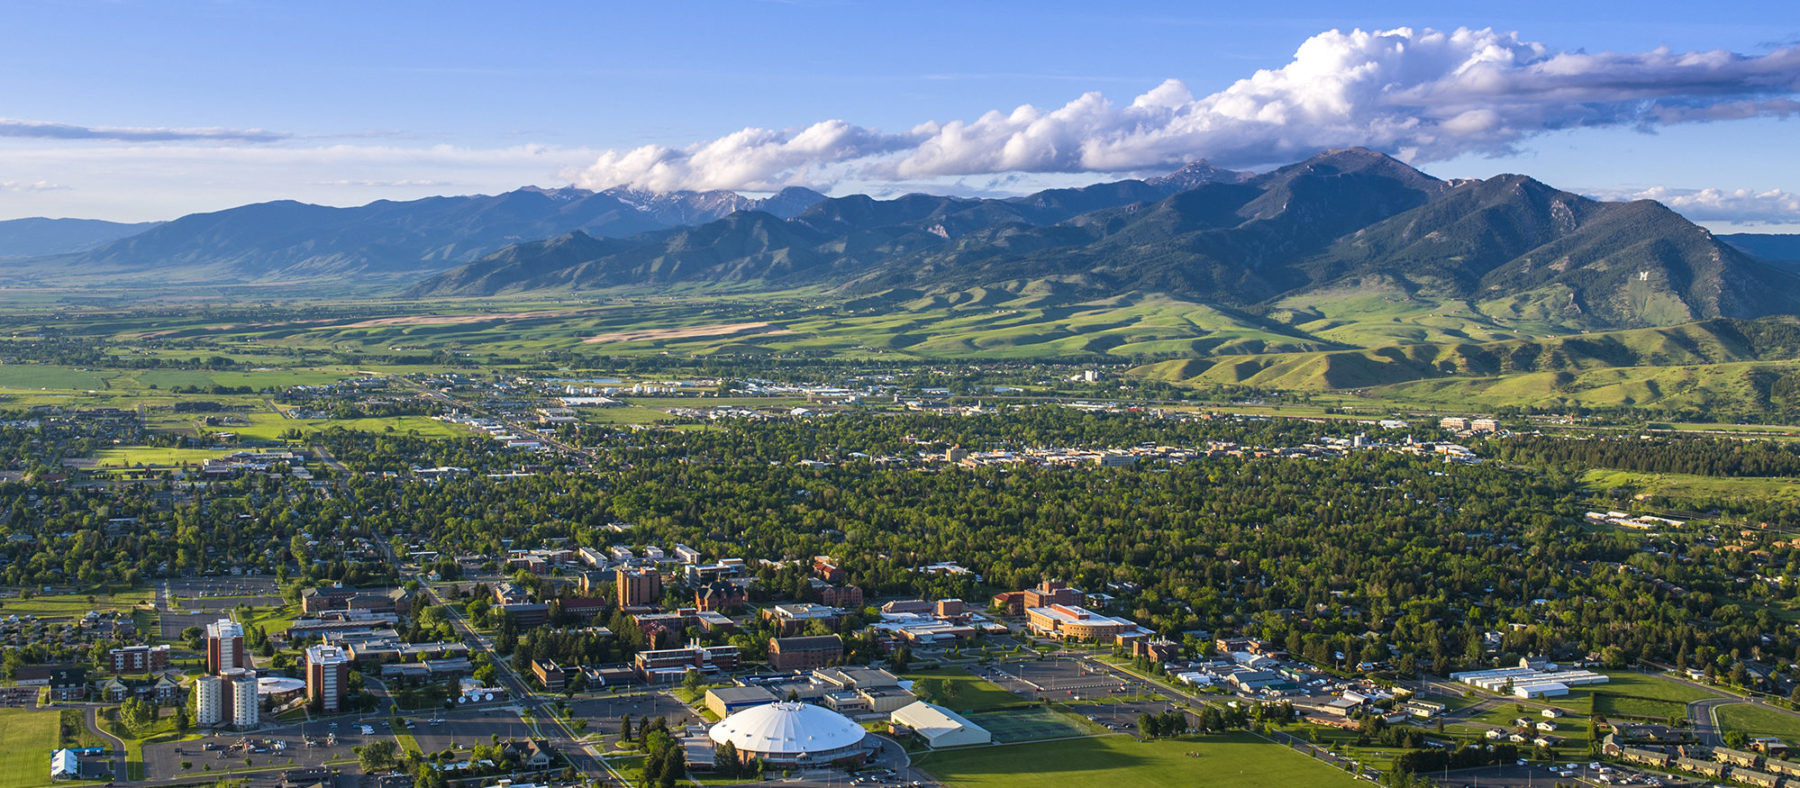
\includegraphics[width=5in,height=\textheight]{images/msu-campus.jpg}}
\usepackage{etoolbox}
\makeatletter
\providecommand{\subtitle}[1]{% add subtitle to \maketitle
  \apptocmd{\@title}{\par {\large #1 \par}}{}{}
}
\makeatother
\subtitle{Fall 2022\\
Montana State University}
\author{Melinda Yager\\
Jade Schmidt\\
Stacey Hancock}
\date{}

\begin{document}
\maketitle

\newpage
\thispagestyle{empty}

This resource was developed by Melinda Yager, Jade Schmidt, and Stacey Hancock in 2021 to accompany the online textbook: Carnegie, N., Hancock, S., Meyer, E., Schmidt, J., and Yager, M. (2021). \emph{Montana State Introductory Statistics with R}. Montana State University. \url{https://mtstateintrostats.github.io/IntroStatTextbook/}.

This resource is released under a \href{https://creativecommons.org/licenses/by-nc-sa/4.0/}{Creative Commons BY-NC-SA 4.0} license unless otherwise noted.

\setcounter{tocdepth}{1}
\addtocontents{toc}{\protect\thispagestyle{empty}}
\tableofcontents
\thispagestyle{empty}

\newpage
\setcounter{page}{1}

\hypertarget{preface}{%
\chapter*{Preface}\label{preface}}
\addcontentsline{toc}{chapter}{Preface}

This coursepack accompanies the textbook for STAT 216: Introduction to Statistics at Montana State University, which can be found at \url{https://mtstateintrostats.github.io/IntroStatTextbook/}. The syllabus for the course (including the course calendar), data sets, and links to D2L Brightspace, Gradescope, and the MSU RStudio server can be found on the course webpage: \url{https://math.montana.edu/courses/s216/}.
Videos assigned in the course calendar and other notes and review materials are linked in D2L.

Each of the activities in this workbook is designed to target specific learning outcomes of the course, giving you practice with important statistical concepts in a group setting with instructor guidance. In addition to the in-class activities for the course, the coursepack includes reading guides to aid in taking notes while you complete the required readings and videos. Bring this workbook with you to class each class period, and take notes in the workbook as you would your own notes. A well-written completed workbook will provide an optimal study guide for exams!

The activities and labs in this coursepack will be completed during class time. Parts of each lab will be turned in on Gradescope. To aid in your understanding, read through the introduction for each activity before attending class each day.

STAT 216 is a 3-credit in-person course. In our experience, it takes six to nine hours per week outside of class to achieve a good grade in this class. By ``good'' we mean at least a C because a grade of D or below does not count toward fulfilling degree requirements. Many of you set your goals higher than just getting a C, and we fully support that. You need roughly nine hours per week to review past activities, read feedback on previous assignments, complete current assignments, and prepare for the next day's class. A typical week in the life of a STAT 216 student looks like:

\begin{itemize}
\tightlist
\item
  \emph{Prior to class meeting}:

  \begin{itemize}
  \tightlist
  \item
    Read assigned sections of the textbook, using the provided reading guides to take notes on the material.
  \item
    Watch assigned videos on that week's content, pausing to take notes and answer video quiz questions.
  \item
    Read through the introduction to the day's in-class activity
  \item
    Read through the week's homework assignment and note any questions you may have on the content.
  \end{itemize}
\item
  \emph{During class meeting}:

  \begin{itemize}
  \tightlist
  \item
    Work through the in-class activity or weekly lab with your classmates and instructor, taking detailed notes on your answers to each question in the activity.
  \end{itemize}
\item
  \emph{After class meeting}:

  \begin{itemize}
  \tightlist
  \item
    Complete any parts of the activity you did not complete in class.
  \item
    Review the activity solutions in the Math and Stat Center, and take notes on key points.
  \item
    Finish watching any remaining assigned videos or readings for the week.
  \item
    Complete the week's homework assignment.
  \end{itemize}
\end{itemize}

\nocite{*}

\hypertarget{fall-2023-calendar-of-in-class-activities}{%
\chapter*{Fall 2023 Calendar of In-Class Activities}\label{fall-2023-calendar-of-in-class-activities}}
\addcontentsline{toc}{chapter}{Fall 2023 Calendar of In-Class Activities}

This calendar only lists the in-class activities, RStudio labs and exams each week. For required readings as well as due dates for assignments, refer to the calendar at:\\
\url{https://mtstateintrostats.github.io/Syllabus/\#Course_calendar}

\begin{longtable}{|l|l|l|l|p{.55\textwidth}|}
\hline
\textbf{Week}& \textbf{Day}& \textbf{Date}& \textbf{Activity} \\ \hline
\endhead

1& W& 8/23& Intro to Data \\*
1& F& 8/25& Data Lecture and Lab \\ \hline
2& M& 8/28& Study Design Lecture - Complete Out of Class Activity 2 \\*
2& W& 8/30& American Indian Address \\* 
2& F& 9/1& Week 2 Lab \\ \hline
3& M& 9/4& (\textit{No class}) \\*
3& W& 9/6& Categorical/Quantitative EDA Lecture - Complete Out of Class Activity 3 \\*
3& F& 9/8& Week 3 Lab \\ \hline
4& M& 9/11& Regression Lecture - Complete Out of Class Activity 4 \\*
4& W& 9/13& Movie Profits \\*
4& F& 9/15& Week 4 Lab \\ \hline
5& M& 9/18& Exam 1 Review \\*
5& W& 9/20& Group Midterm Exam 1 \\*    
5& F& 9/21& Midterm Exam 1 \\ \hline
6& M& 9/26& Hypothesis Testing Lecture \\*
6& W& 9/28& Helper Hinderer --- Simulation HT \\*   
6& F& 9/30& Week 6 Lab \\ \hline
7& M& 10/3& Theory-based Testing Lecture \\*
7& W& 10/5& Handedness of Male Boxers --- Theory\\*
7& F& 10/7& Week 7 Lab \\ \hline
8& M& 10/10& Two Proportion Simulation Lecture \\*
8& W& 10/12& Good Samaritan --- Simulation HT & CI \\*  
8& F& 10/14& Week 8 Lab \\ \hline
9& M& 10/17& Two Proportion Theory Lecture \\*
9& W& 10/19& Helmet Use and Head Injuries --- Theory HT & CI \\*    
9& F& 10/21& Week 9 Lab \\ \hline
10& M& 10/24& Exam 2 Review \\*
10& W& 10/26& Group Midterm Exam 2 \\*
10& F& 10/28& Midterm Exam 2\\ \hline
11& M& 10/31& Paired Inference Lecture \\*
11& W& 11/2& Color Interference \\* 
11& F& 11/4& Week 11 Lab \\ \hline
12& M& 11/7& Weather Patterns and Snowfall \\*
12& W& 11/9& Week 12 Lab \\*
12& F& 11/11& (\textit{No class}) \\ \hline
13& M& 11/14& Regression Inference Lecture \\*
13& W& 11/16& Golf Driving Distances \\*
13& F& 11/18& Week 13 Lab \\ \hline
Holiday& M--F& 11/21--11/25& \textbf{No Class --- Fall Break} \\ \hline
14& M& 11/28& Probability & Relative Risk Lecture \\*
14& W& 11/30& Relative Risk \\*
14& F& 12/2& Week 14 Lab \\ \hline
15& M& 12/5& Final Exam Review \\*
15& W& 12/7& Final Group Exam Part 1 \\*
15& F& 12/9& Final Group Exam Part 2 \\ \hline
Finals& 12/13& 6 - 7:50 pm & Common Final Exam \\
&  &  & See \url{www.montana.edu/registrar/Schedules.html} \\ \hline

\end{longtable}

\nocite{*}

\hypertarget{inference-for-a-single-categorical-variable-simulation-based-methods}{%
\chapter{Inference for a Single Categorical Variable: Simulation-based Methods}\label{inference-for-a-single-categorical-variable-simulation-based-methods}}

\hypertarget{module-6-reading-guide-categorical-inference}{%
\section{Module 6 Reading Guide: Categorical Inference}\label{module-6-reading-guide-categorical-inference}}

\hypertarget{section-5.1-foundations-of-inference-hypothesis-tests}{%
\subsection*{Section 5.1 (Foundations of inference: Hypothesis tests)}\label{section-5.1-foundations-of-inference-hypothesis-tests}}
\addcontentsline{toc}{subsection}{Section 5.1 (Foundations of inference: Hypothesis tests)}

Please note that Theory-based inference will be covered next week.

\textbf{Videos}

\begin{itemize}
\tightlist
\item
  5.1
\end{itemize}

\setstretch{1.25}

\hypertarget{vocabulary}{%
\subsubsection*{Vocabulary}\label{vocabulary}}
\addcontentsline{toc}{subsubsection}{Vocabulary}

Statistical inference:
\rgs

Hypothesis test:

\rgi Also called a `significance test'.
\rgs

Simulation-based method:
\rgs

Theory-based method:
\rgs

Central Limit Theorem:
\rgs

Sampling distribution:
\rgs

Standard deviation of a statistic:
\rgs

Standard error of a statistic:
\rgs

Null hypothesis (\(H_0\)):
\rgs

Alternative hypothesis (\(H_A\)):
\rgs

P-value:
\rgs

Point estimate:
\rgs

Test statistic:
\rgs

Decision:
\rgs

Significance level (\(\alpha\)):
\rgs 

Statistically significant:
\rgs

Confidence interval:
\rgs

Margin of error:
\rgs

\hypertarget{notes}{%
\subsubsection*{Notes}\label{notes}}
\addcontentsline{toc}{subsubsection}{Notes}

What `theory' is behind the theory-based methods of analysis?
\rgs

Consider the US judicial system:

\rgi What is the null hypothesis?
\rgs

\rgi What is the alternative hypothesis?
\rgs

\rgi The jury is presented with evidence.

~~~~~~~~~- If the evidence is strong (beyond a reasonable doubt), the jury will find the defendant:

\rgs

~~~~~~~~~- If the evidence is not strong (not beyond a reasonable doubt), the jury will find the defendant:

\rgs

To create a simulation, which hypothesis (null or alternative) do we assume is true?
\rgs

More on p-values:

\rgi Lower the p-value:
\rgs

\rgi Interpretations require:
\rgs

General steps of a hypothesis test:
\rgs

Conclusions should include:
\rgs

Decision:

\rgi If p-value \(\leq \alpha\), the decision is to:

\rgi If p-value \(> \alpha\), the decision is to:

True or False: If the p-value is above 0.10, that means the null hypothesis is true.

True or False: When conducting a simulation-based hypothesis test, the null hypothesis is assumed to be true to create the simulation.

\hypertarget{formulas}{%
\subsubsection*{Formulas}\label{formulas}}
\addcontentsline{toc}{subsubsection}{Formulas}

\(SD(\hat{p})\) =
\rgs

General form of a theory-based confidence interval:
\rgs

Margin of error:
\rgs

\hypertarget{example-martian-alphabet}{%
\subsubsection*{Example: Martian alphabet}\label{example-martian-alphabet}}
\addcontentsline{toc}{subsubsection}{Example: Martian alphabet}

\begin{enumerate}
\def\labelenumi{\arabic{enumi}.}
\item
  What is the sample statistic presented in this example? What notation would be used to represent this value?
  \rgs
\item
  What are the two possible explanations for how these data could have occurred?
  \rgs
  \rgs
\item
  Of the two explanations, which is the null and which is the alternative hypothesis?
  \rgs
\item
  How could coins be used to create a simulation of what should happen if everyone in the class was just guessing?
  \rgs
  \rgs
  \rgs
\item
  How can we use the simulation to determine which of the two possibilities is more believable?
  \rgs
  \rgs
\item
  What decision should be made at an \(\alpha = 0.05\) significance level? Justify your answer.
  \rgs
\item
  Are the results in this example statistically significant? Justify your answer.
  \rgs
\item
  Interpret the 95\% confidence interval provided in the textbook.
  \rgs
  \rgs
\item
  The formula for the interval is \(34/38 \pm (2 \times 0.08) = 0.89 \pm 0.16\). Calculating that, you should get (0.73, 1.05). Why was the interval shown in the textbook (0.73, 1) instead of (0.73, 1.05)?
  \rgs
\end{enumerate}

\hypertarget{section-5.3-inference-for-one-proportion}{%
\subsection*{Section 5.3 (Inference for one proportion)}\label{section-5.3-inference-for-one-proportion}}
\addcontentsline{toc}{subsection}{Section 5.3 (Inference for one proportion)}

\setstretch{1}

You may skip Section 5.3.4, which will be covered next week.

\textbf{Videos}

\begin{itemize}
\tightlist
\item
  5.3SimInf
\item
  Bootstrapping
\end{itemize}

\hypertarget{reminders-from-previous-sections}{%
\subsubsection*{Reminders from previous sections}\label{reminders-from-previous-sections}}
\addcontentsline{toc}{subsubsection}{Reminders from previous sections}

\(n\) = sample size

\(\hat{p}\) = sample proportion

\(\pi\) = population proportion

General steps of a hypothesis test:

\begin{enumerate}
\def\labelenumi{\arabic{enumi}.}
\item
  Frame the research question in terms of hypotheses.
\item
  Collect and summarize data using a test statistic.
\item
  Assume the null hypothesis is true, and simulate or mathematically model a null distribution for the test statistic.
\item
  Compare the observed test statistic to the null distribution to calculate a p-value.
\item
  Make a conclusion based on the p-value and write the conclusion in context.
\end{enumerate}

Parameter: a value summarizing a variable(s) for a population.

Statistic: a value summarizing a variable(s) for a sample.

Sampling distribution: plot of statistics from 1000s of samples of the same size taken from the same population.

Standard deviation of a statistic: the variability of statistics from 1000s of samples; how far, on average, each statistic is from the true value of the parameter.

Standard error of a statistic: estimated standard deviation of a statistic.

Hypothesis test: a process to determine how strong the evidence of an effect is.

\rgi Also called a `significance test'.

Simulation-based method: Simulate lots of samples of size \(n\) under assumption of the null hypothesis, then find the proportion of the simulations that are at least as extreme as the observed sample statistic.

Null hypothesis (\(H_0\)): the skeptical perspective; no difference; no change; no effect; random chance; what the researcher hopes to prove is \textbf{wrong}.

Alternative hypothesis (\(H_A\)): the new perspective; a difference/increase/decrease; an effect; not random chance; what the researcher hopes to prove is \textbf{correct}.

P-value: probability of seeing the observed sample data, or something more extreme, assuming the null hypothesis is true.

\(\implies\) Lower the p-value the stronger the evidence AGAINST the null hypothesis and FOR the alternative hypothesis.

Decision: a determination of whether to `reject' or `fail to reject' a null hypothesis based on a p-value and a pre-set level of significance.

Significance level (\(\alpha\)): a threshold used to determine if a p-value provides enough evidence to reject the null hypothesis or not.

\rgi Common levels of \(\alpha\) include 0.01, 0.05, and 0.10.

Statistically significant: results are considered statistically significant if the p-value is below the significance level.

Confidence interval: a process to determine how large an effect is; a range of plausible values for the parameter; also called `estimation'.

Margin of error: the value that is added to and subtracted from the sample statistic to create a confidence interval; half the width of a confidence interval.

\hypertarget{vocabulary-1}{%
\subsubsection*{Vocabulary}\label{vocabulary-1}}
\addcontentsline{toc}{subsubsection}{Vocabulary}

Point estimate:
\rgs

Test statistic:
\rgs

Null value:
\rgs

Null distribution:
\rgs

One-sided hypothesis test:
\rgs

Two-sided hypothesis test:
\rgs

Bootstrapping:
\rgs

Bootstrapped resample:
\rgs

Bootstrapped statistic:
\rgs

\hypertarget{notes-1}{%
\subsubsection*{Notes}\label{notes-1}}
\addcontentsline{toc}{subsubsection}{Notes}

Which hypothesis must we assume is true in order to simulate a null distribution?
\rgs

Explain the differences between a one-sided and two-sided hypothesis test.
\vspace{1mm}

\rgi How will the research questions differ?
\rgs

\rgi How will the notation in the alternative hypothesis differ?
\rgs

\rgi How does the p-value calculation differ?
\rgs

How does the p-value in a two-sided test compare to the p-value in a one-sided test?
\rgs

Should the default in research be a one-sided or two-sided hypothesis test? Explain why.
\rgs
\rgs

Purpose of bootstrapping:
\rgs

How is bootstrapping used?\\
\rgs

If we want to find a 90\% confidence interval, what percentiles of the bootstrap distribution would we need?\\
\rgs

\hypertarget{example-organ-donations}{%
\subsubsection*{Example: Organ donations}\label{example-organ-donations}}
\addcontentsline{toc}{subsubsection}{Example: Organ donations}

\begin{enumerate}
\def\labelenumi{\arabic{enumi}.}
\item
  What is the sample statistic presented in this example? What notation would be used to represent this value?
  \rgs
\item
  What is the parameter representing in the context of this problem? What notation would be used to represent this parameter?
  \rgs
  \rgs
\item
  Write the null and alternative hypotheses in words, using the example in 5.3.1.
  \rgs
  \rgs
\item
  Write the null and alternative hypotheses in notation, using the example in 5.3.1.
  \rgs
\item
  To simulate the null distribution, we would not be able to use coins. Why not?
  \rgs
  \rgs
\item
  How could we use cards to simulate 1 sample which assumes the null hypothesis is true? How many blue cards --- to represent what? How many red cards --- to represent what? How many times would we draw a card and replace it back in the deck? What would you record once you completed the draw-with-replacement process?
  \rgs
  \rgs
  \rgs
\item
  How can we calculate a p-value from the simulated null distribution for this example in 5.3.1?
  \rgs
  \rgs
\item
  What was the p-value of the test from the example in 5.3.1?
  \rgs
\item
  At the 5\% significance level, what decision would you make based on the p-value above?
  \rgs
\item
  What conclusion should the researcher make?
  \rgs
  \rgs
\item
  Are the results in this example statistically significant? Justify your answer.
  \rgs
  \rgs
\item
  How does the alternative hypothesis change, both in words and in notation, when the example changes to a two-sided hypothesis test in 5.3.2?\\
  \rgs
  \rgs
\item
  Explain how the p-value calculation changes between the example in 5.3.1 (one-sided hypothesis test) and the example in 5.3.2 (two-sided hypothesis test).
  \rgs
  \rgs
\item
  Why does doubling the p-value from the one-sided hypothesis test (your answer to question 8) not match the two-sided p-value calculated in Figure 5.12?
  \rgs
  \rgs
\item
  How could we use cards to simulate \textbf{one} bootstrapped resample? How many blue cards --- to represent what? How many red cards --- to represent what? How many times would we draw a card and replace it back in the deck? What would you record once you completed the draw-with-replacement process?
  \rgs
  \rgs
  \rgs
\item
  Interpret the 95\% confidence interval provided in the textbook.
  \rgs
  \rgs
\item
  Are the results in this example statistically significant? Justify your answer.
  \rgs
\end{enumerate}

\newpage

\hypertarget{lecture-notes-week-6-inference-for-one-categorical-variable-using-simulation-based-methods}{%
\section{Lecture Notes Week 6: Inference for one categorical variable using Simulation-based methods}\label{lecture-notes-week-6-inference-for-one-categorical-variable-using-simulation-based-methods}}

\setstretch{1}

\hypertarget{hypothesis-testing}{%
\subsection{Hypothesis Testing}\label{hypothesis-testing}}

Purpose of a hypothesis test:

\begin{itemize}
\item
  Use data collected on a \_\_\_\_\_\_\_\_\_\_\_\_\_\_\_\_\_\_\_\_ to give information about the \_\_\_\_\_\_\_\_\_\_\_\_\_\_\_
\item
  Determines \_\_\_\_\_\_\_\_\_\_\_\_\_\_\_\_\_\_ of \_\_\_\_\_\_\_\_\_\_\_\_\_\_\_\_\_\_\_\_\_ of an effect
\end{itemize}

General steps of a hypothesis test

\begin{enumerate}
\def\labelenumi{\arabic{enumi}.}
\item
  Write a research question and hypotheses.
\item
  Collect data and calculate a summary statistic.
\item
  Model a sampling distribution which assumes the null hypothesis is true.
\item
  Calculate a p-value.
\item
  Draw conclusions based on a p-value.
\end{enumerate}

\hypertarget{hypotheses}{%
\subsection*{Hypotheses}\label{hypotheses}}
\addcontentsline{toc}{subsection}{Hypotheses}

\begin{itemize}
\tightlist
\item
  Two possible outcomes:
\end{itemize}

\vspace{1in}

\begin{itemize}
\tightlist
\item
  Always written about the \_\_\_\_\_\_\_\_\_\_\_\_\_\_\_\_\_\_ (population)
\end{itemize}

\hypertarget{null-hypothesis}{%
\subsubsection*{Null hypothesis}\label{null-hypothesis}}
\addcontentsline{toc}{subsubsection}{Null hypothesis}

\begin{itemize}
\item
  Skeptical perspective, no difference, no effect, random chance
\item
  What the researcher hopes is \_\_\_\_\_\_\_\_\_\_\_\_\_\_\_.
\end{itemize}

Notation:

\vspace{0.1in}

\hypertarget{alternative-hypothesis}{%
\subsubsection*{Alternative hypothesis}\label{alternative-hypothesis}}
\addcontentsline{toc}{subsubsection}{Alternative hypothesis}

\begin{itemize}
\item
  New perspective, a chance, a difference, an effect
\item
  What the researcher hopes is \_\_\_\_\_\_\_\_\_\_\_\_\_\_\_\_.
\end{itemize}

Notation:

\vspace{0.1in}

\hypertarget{simulation-vs.-theory-based-methods}{%
\subsection*{Simulation vs.~Theory-based Methods}\label{simulation-vs.-theory-based-methods}}
\addcontentsline{toc}{subsection}{Simulation vs.~Theory-based Methods}

\hypertarget{simulation-based-method}{%
\subsubsection*{Simulation-based method}\label{simulation-based-method}}
\addcontentsline{toc}{subsubsection}{Simulation-based method}

\setstretch{1.5}

Creation of the null distribution

\begin{itemize}
\tightlist
\item
  Simulate many samples assuming
\end{itemize}

\vspace{0.2in}

\begin{itemize}
\item
  Find the proportion of \_\_\_\_\_\_\_\_\_\_\_\_\_\_\_\_\_\_\_ at least as extreme as the observed sample \_\_\_\_\_\_\_\_\_\_\_\_
\item
  The null distribution estimates the sample to sample \_\_\_\_\_\_\_\_\_\_\_\_\_\_\_\_\_\_\_\_ expected in the population
\end{itemize}

\setstretch{1}

\hypertarget{theory-based-method}{%
\subsubsection*{Theory-based method}\label{theory-based-method}}
\addcontentsline{toc}{subsubsection}{Theory-based method}

\begin{itemize}
\item
  Use a mathematical model to determine a distribution under the null hypothesis
\item
  Compare the observed sample statistic to the model to calculate a probability
\item
  \emph{Theory-based methods will be discussed next week}
\end{itemize}

\hypertarget{p-value}{%
\subsubsection*{P-value}\label{p-value}}
\addcontentsline{toc}{subsubsection}{P-value}

\setstretch{1.5}

\begin{itemize}
\item
  What does the p-value measure?

  \begin{itemize}
  \tightlist
  \item
    Probability of observing the sample \_\_\_\_\_\_\_\_\_\_\_\_\_\_\_\_\_\_\_ or more \_\_\_\_\_\_\_\_\_\_\_\_\_\_\_\_
    assuming the \_\_\_\_\_\_\_\_ hypothesis is \_\_\_\_\_\_\_\_\_\_.
  \end{itemize}
\item
  How much evidence does the p-value provide against the null hypothesis?
\end{itemize}

\begin{center}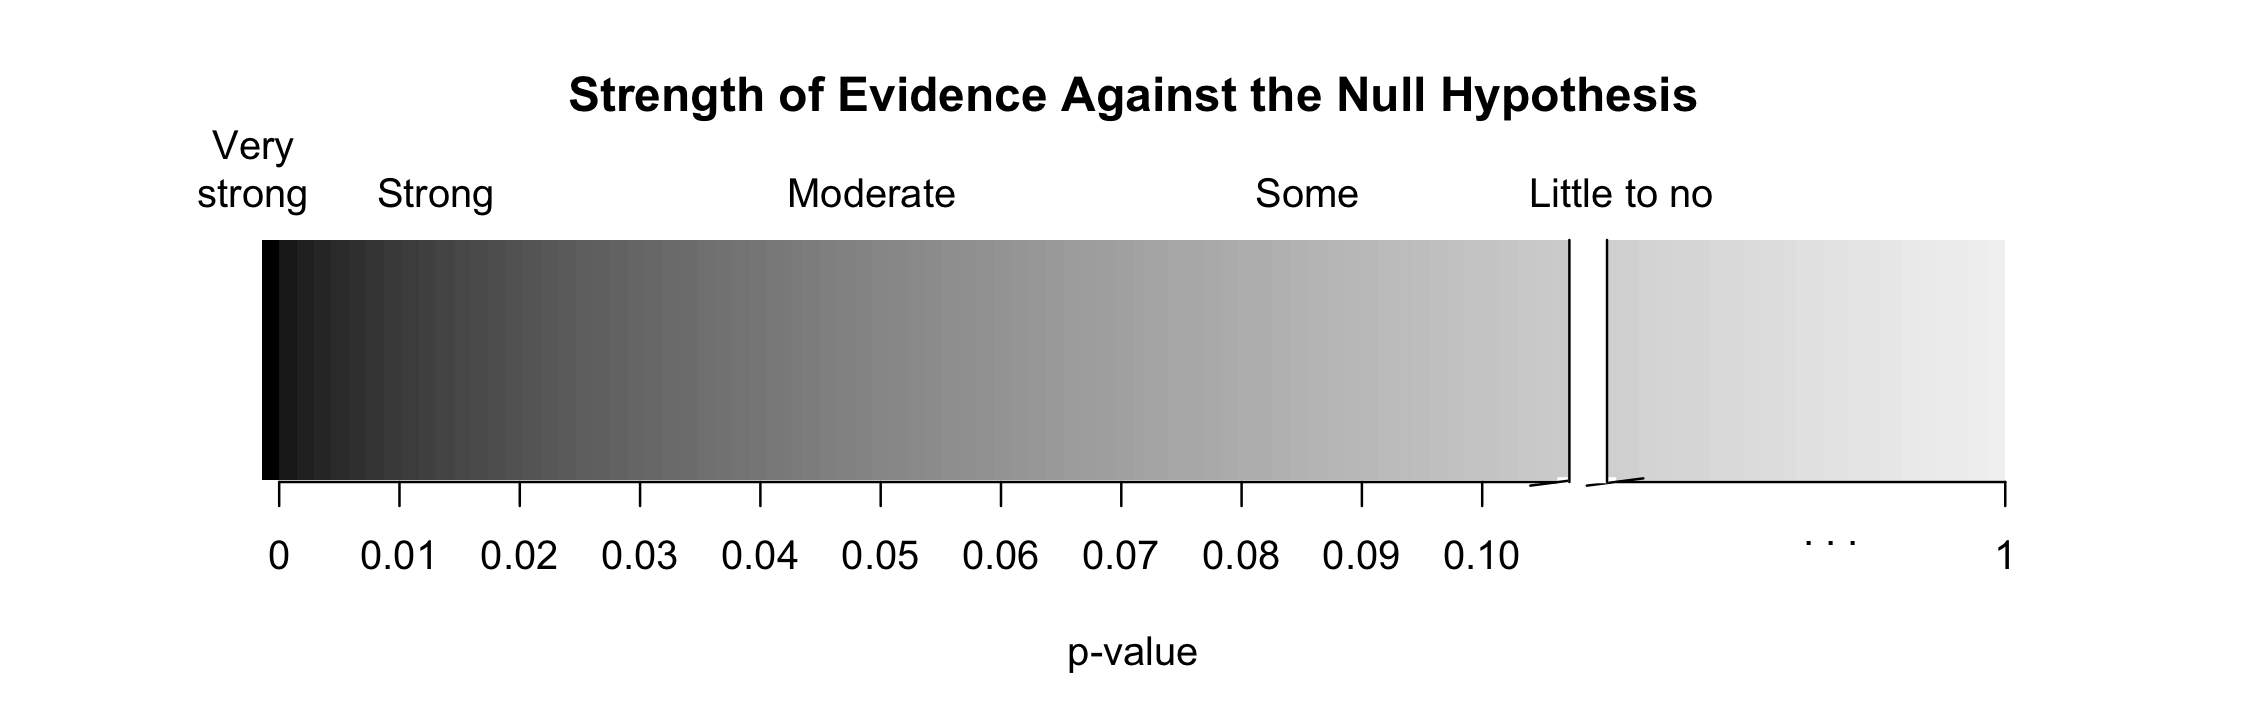
\includegraphics[width=0.9\linewidth]{images/soe_gradient_gray} \end{center}

\vspace{0.5mm}

\rgi \rgi - The \_\_\_\_\_\_\_\_\_\_\_\_\_\_\_\_\_\_the p-value, the \_\_\_\_\_\_\_\_\_\_\_\_\_\_\_\_\_\_\_ the evidence against the null hypothesis.

\begin{itemize}
\tightlist
\item
  Write a conclusion based on the p-value.
\end{itemize}

\rgi \rgi - Answers the \_\_\_\_\_\_\_\_\_\_\_\_\_\_\_\_ question.

\rgi \rgi - Amount of \_\_\_\_\_\_\_\_\_\_\_\_\_\_\_\_\_ in support of the \_\_\_\_\_\_\_\_\_\_\_\_\_\_\_\_\_ hypothesis.

\begin{itemize}
\tightlist
\item
  Decision: can we reject or fail to reject the null hypothesis?
\end{itemize}

\rgi - Significance level: cut-off of ``small'' vs ``large'' p-value

\rgi \rgi - \(\text{p-value} \le \alpha\)

\rgi \rgi \rgi - Strong enough evidence against the null hypothesis

\rgi \rgi \rgi - Decision:

\vspace{0.2in}

\rgi \rgi \rgi - Results are \_\_\_\_\_\_\_\_\_\_\_\_\_\_\_\_\_\_\_\_\_\_\_ significant.

\rgi \rgi - \(\text{p-value} > \alpha\)

\rgi \rgi \rgi - Not enough evidence against the null hypothesis

\rgi \rgi \rgi - Decision:

\vspace{0.2in}

\rgi \rgi \rgi - Results are not \_\_\_\_\_\_\_\_\_\_\_\_\_\_\_\_\_\_\_\_\_ significant.

\hypertarget{one-proportion-test}{%
\subsection*{One proportion test}\label{one-proportion-test}}
\addcontentsline{toc}{subsection}{One proportion test}

\begin{itemize}
\item
  Reminder: review summary measures and plots discussed in the Week 3 material and Chapter 4 of the textbook.
\item
  The summary measure for a single categorical variable is a \_\_\_\_\_\_\_\_\_\_\_\_\_\_.
\end{itemize}

Notation:

\begin{itemize}
\item
  Population proportion:
\item
  Sample proportion:
\end{itemize}

\newpage

Parameter of Interest:

\begin{itemize}
\item
  Include:

  \begin{itemize}
  \item
    Reference of the population (true, long-run, population, all)
  \item
    Summary measure
  \item
    Context

    \begin{itemize}
    \item
      Observational units/cases
    \item
      Response variable (and explanatory variable if present)

      \begin{itemize}
      \tightlist
      \item
        If the response variable is categorical, define a `success' in context
      \end{itemize}
    \end{itemize}
  \end{itemize}
\end{itemize}

\(\pi:\)

\vspace{0.5in}

\hypertarget{hypothesis-testing-1}{%
\subsubsection*{Hypothesis testing}\label{hypothesis-testing-1}}
\addcontentsline{toc}{subsubsection}{Hypothesis testing}

Conditions:

\begin{itemize}
\tightlist
\item
  Independence:
\end{itemize}

\vspace{0.3in}

Null hypothesis assumes ``no effect'', ``no difference'', ``nothing interesting happening'', etc.

\rgi Always of form: ``parameter'' = null value

\(H_0:\)

\vspace{0.5in}

\(H_A:\)

\vspace{0.5in}

\begin{itemize}
\tightlist
\item
  Research question determines the alternative hypothesis.
\end{itemize}

Example: A 2007 study published in the Behavioral Ecology and Sociobiology journal was titled ``Why do blue-eyed men prefer blue-eyed women?'' In this study, conducted in Norway, 114 volunteer heterosexual blue-eyed males rated the attractiveness of 120 pictures of females. The researchers recorded which eye-color (blue, green, or brown) was rated the highest, on average. In the sample, 51 of the volunteers rated the blue-eyed women the most attractive. Do blue-eyed heterosexual men tend to find blue-eyed women the most attractive?

Parameter of interest:

\vspace{0.6in}

Write the null and alternative hypotheses for the blue-eyed study:

In words:

\(H_0:\)

\vspace{0.5in}

\(H_A:\)

\vspace{0.5in}

In notation:

\(H_0:\)

\vspace{0.2in}

\(H_A:\)

\vspace{0.2in}

Statistic:

\vspace{0.2in}

Is the independence condition met to analyze these data using a simulation-based approach?

\vspace{0.3in}

\hypertarget{simulation-based-method-1}{%
\subsubsection*{Simulation-based method}\label{simulation-based-method-1}}
\addcontentsline{toc}{subsubsection}{Simulation-based method}

\begin{itemize}
\item
  Simulate many samples assuming \(H_0: \pi = \pi_0\)

  \begin{itemize}
  \item
    Create a spinner with that represents the null value
  \item
    Spin the spinner \(n\) times
  \item
    Calculate and plot the simulated sample proportion from each simulation
  \item
    Repeat 1000 times (simulations) to create the null distribution
  \item
    Find the proportion of simulations at least as extreme as \(\hat{p}\)
  \end{itemize}
\end{itemize}

\begin{Shaded}
\begin{Highlighting}[]
\FunctionTok{set.seed}\NormalTok{(}\DecValTok{216}\NormalTok{)}
\FunctionTok{one\_proportion\_test}\NormalTok{(}\AttributeTok{probability\_success =} \FloatTok{0.333}\NormalTok{, }\CommentTok{\# Null hypothesis value}
          \AttributeTok{sample\_size =} \DecValTok{114}\NormalTok{, }\CommentTok{\# Enter sample size}
          \AttributeTok{number\_repetitions =} \DecValTok{1000}\NormalTok{, }\CommentTok{\# Enter number of simulations}
          \AttributeTok{as\_extreme\_as =} \FloatTok{0.447}\NormalTok{, }\CommentTok{\# Observed statistic}
          \AttributeTok{direction =} \StringTok{"greater"}\NormalTok{, }\CommentTok{\# Specify direction of alternative hypothesis}
          \AttributeTok{summary\_measure =} \StringTok{"proportion"}\NormalTok{) }\CommentTok{\# Reporting proportion or number of successes?}
\end{Highlighting}
\end{Shaded}

\begin{center}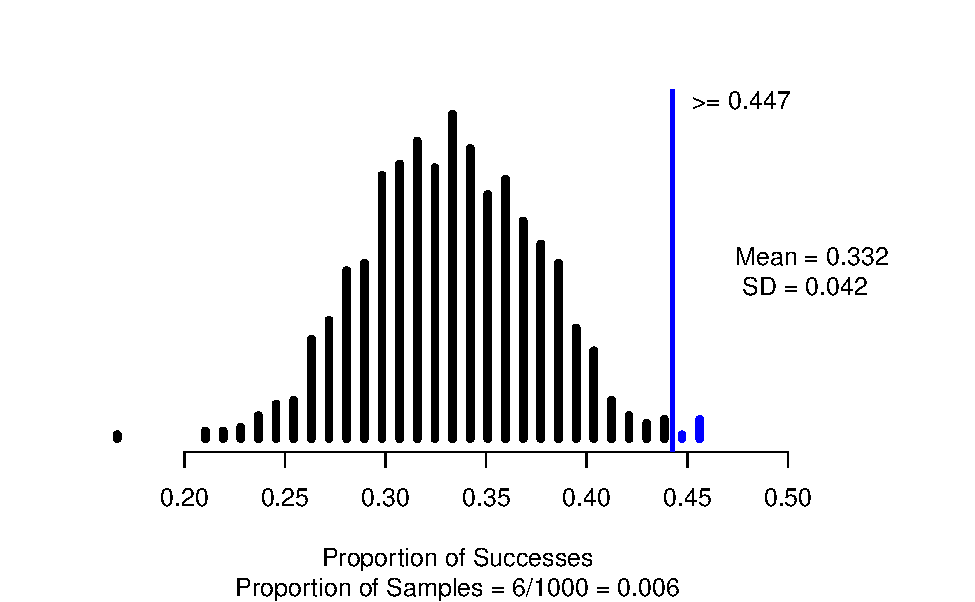
\includegraphics[width=0.7\linewidth]{06-LN06-1cat_simulation_files/figure-latex/unnamed-chunk-2-1} \end{center}

Explain why the null distribution is centered at the value of approximately 0.333:

\vspace{0.5in}

Interpretation of the p-value:

\begin{itemize}
\item
  Statement about probability or proportion of samples
\item
  Statistic (summary measure and value)
\item
  Direction of the alternative
\item
  Null hypothesis (in context)
\end{itemize}

\vspace{0.8in}

Conclusion:

\begin{itemize}
\item
  Amount of evidence
\item
  Parameter of interest
\item
  Direction of the alternative hypothesis
\end{itemize}

\vspace{0.6in}

Generalization:

\begin{itemize}
\tightlist
\item
  Can the results of the study be generalized to the target population?
\end{itemize}

\vspace{0.4in}

\hypertarget{confidence-interval}{%
\subsection*{Confidence interval}\label{confidence-interval}}
\addcontentsline{toc}{subsection}{Confidence interval}

\rgi \(\text{statistic} \pm \text{margin of error}\)

Vocabulary:

\begin{itemize}
\tightlist
\item
  Point estimate:
\end{itemize}

\vspace{0.3in}

\begin{itemize}
\tightlist
\item
  Margin of error:
\end{itemize}

\vspace{0.3in}

\setstretch{1.5}

Purpose of a confidence interval

\begin{itemize}
\item
  To give an \_\_\_\_\_\_\_\_\_\_\_\_\_\_\_\_\_\_\_\_ \_\_\_\_\_\_\_\_\_\_\_\_\_\_\_\_\_\_\_ for the parameter of interest
\item
  Determines how \_\_\_\_\_\_\_\_\_\_\_\_\_\_ an effect is
\end{itemize}

\setstretch{1}

\hypertarget{sampling-distribution}{%
\subsubsection*{Sampling distribution}\label{sampling-distribution}}
\addcontentsline{toc}{subsubsection}{Sampling distribution}

\setstretch{1.5}

\begin{itemize}
\item
  Ideally, we would take many samples of the same \_\_\_\_\_\_\_\_\_\_\_ from the same population to create a sampling distribution
\item
  But only have 1 sample, so we will \_\_\_\_\_\_\_\_\_\_\_\_\_\_\_\_\_ with \_\_\_\_\_\_\_\_\_\_\_\_\_\_\_\_\_ from the one sample.
\item
  Need to estimate the sampling distribution to see the \_\_\_\_\_\_\_\_\_\_\_\_\_\_\_\_\_ in the sample
\end{itemize}

\setstretch{1}

\hypertarget{simulation-based-methods}{%
\subsubsection*{Simulation-based methods}\label{simulation-based-methods}}
\addcontentsline{toc}{subsubsection}{Simulation-based methods}

Bootstrap distribution:

\begin{itemize}
\item
  Write the response variable values on cards
\item
  Sample with replacement \(n\) times (bootstrapping)
\item
  Calculate and plot the simulated difference in sample means from each simulation
\item
  Repeat 1000 times (simulations) to create the bootstrap distribution
\item
  Find the cut-offs for the middle X\% (confidence level) in a bootstrap distribution.
\end{itemize}

What is bootstrapping?

\begin{itemize}
\item
  Assume the ``population'' is many, many copies of the original sample.
\item
  Randomly sample with replacement from the original sample \(n\) times.
\end{itemize}

\newpage

Let's revisit the blue-eyed male study to estimate the \emph{proportion of ALL heterosexual blue-eyed males who tend to find blue-eyed women the most attractive} by creating a 90\% confidence interval.

Bootstrap distribution:

\begin{Shaded}
\begin{Highlighting}[]
\FunctionTok{set.seed}\NormalTok{(}\DecValTok{216}\NormalTok{)}
\FunctionTok{one\_proportion\_bootstrap\_CI}\NormalTok{(}\AttributeTok{sample\_size =} \DecValTok{114}\NormalTok{, }\CommentTok{\# Sample size}
                    \AttributeTok{number\_successes =} \DecValTok{51}\NormalTok{, }\CommentTok{\# Observed number of successes}
                    \AttributeTok{number\_repetitions =} \DecValTok{1000}\NormalTok{, }\CommentTok{\# Number of bootstrap samples to use}
                    \AttributeTok{confidence\_level =} \FloatTok{0.90}\NormalTok{) }\CommentTok{\# Confidence level as a decimal}
\end{Highlighting}
\end{Shaded}

\begin{center}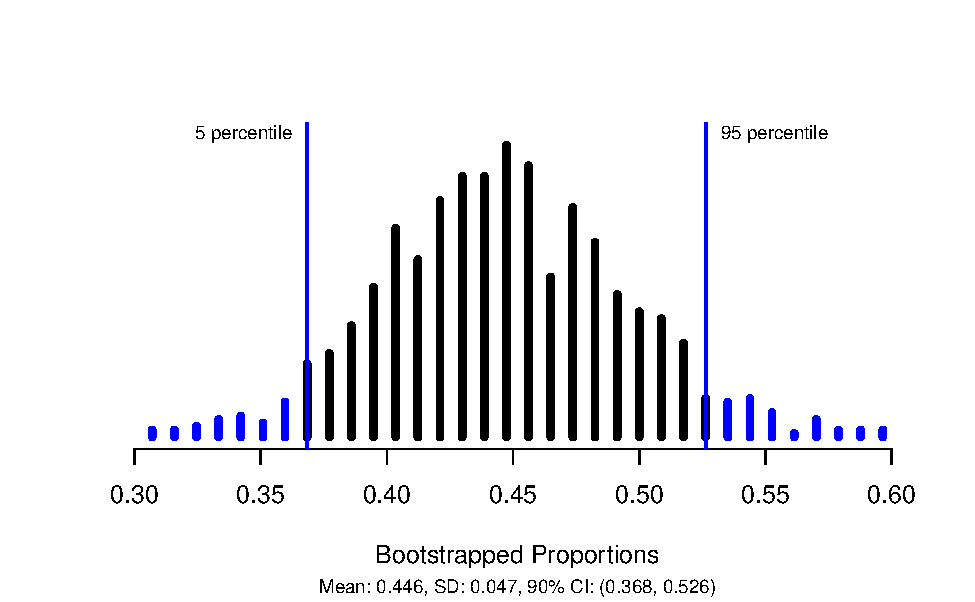
\includegraphics[width=0.7\linewidth]{06-LN06-1cat_simulation_files/figure-latex/unnamed-chunk-3-1} \end{center}

Confidence interval interpretation:

\begin{itemize}
\item
  How confident you are (e.g., 90\%, 95\%, 98\%, 99\%)
\item
  Parameter of interest
\item
  Calculated interval
\item
  Order of subtraction when comparing two groups
\end{itemize}

\vspace{0.8in}

Do the results of the confidence interval \emph{match} the results based on the p-value?

\vspace{0.5in}

How does changing the confidence level impact the width of the confidence interval?

95\% Confidence Interval:

\begin{Shaded}
\begin{Highlighting}[]
\FunctionTok{set.seed}\NormalTok{(}\DecValTok{216}\NormalTok{)}
\FunctionTok{one\_proportion\_bootstrap\_CI}\NormalTok{(}\AttributeTok{sample\_size =} \DecValTok{114}\NormalTok{, }\CommentTok{\# Sample size}
                    \AttributeTok{number\_successes =} \DecValTok{51}\NormalTok{, }\CommentTok{\# Observed number of successes}
                    \AttributeTok{number\_repetitions =} \DecValTok{1000}\NormalTok{, }\CommentTok{\# Number of bootstrap samples to use}
                    \AttributeTok{confidence\_level =} \FloatTok{0.95}\NormalTok{) }\CommentTok{\# Confidence level as a decimal}
\end{Highlighting}
\end{Shaded}

\begin{center}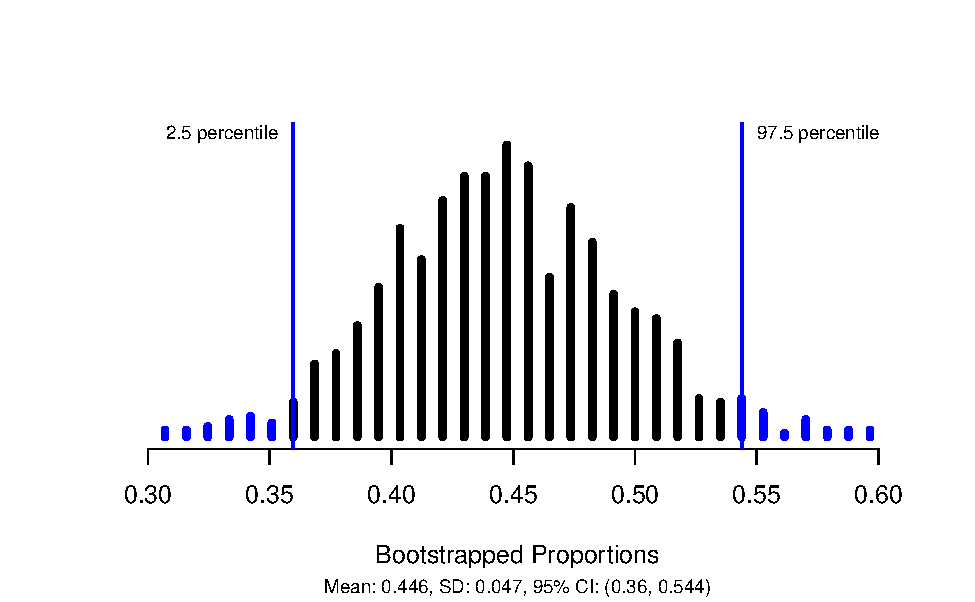
\includegraphics[width=0.7\linewidth]{06-LN06-1cat_simulation_files/figure-latex/unnamed-chunk-4-1} \end{center}

99\% Confidence Interval:

\begin{Shaded}
\begin{Highlighting}[]
\FunctionTok{set.seed}\NormalTok{(}\DecValTok{216}\NormalTok{)}
\FunctionTok{one\_proportion\_bootstrap\_CI}\NormalTok{(}\AttributeTok{sample\_size =} \DecValTok{114}\NormalTok{, }\CommentTok{\# Sample size}
                    \AttributeTok{number\_successes =} \DecValTok{51}\NormalTok{, }\CommentTok{\# Observed number of successes}
                    \AttributeTok{number\_repetitions =} \DecValTok{1000}\NormalTok{, }\CommentTok{\# Number of bootstrap samples to use}
                    \AttributeTok{confidence\_level =} \FloatTok{0.99}\NormalTok{) }\CommentTok{\# Confidence level as a decimal}
\end{Highlighting}
\end{Shaded}

\begin{center}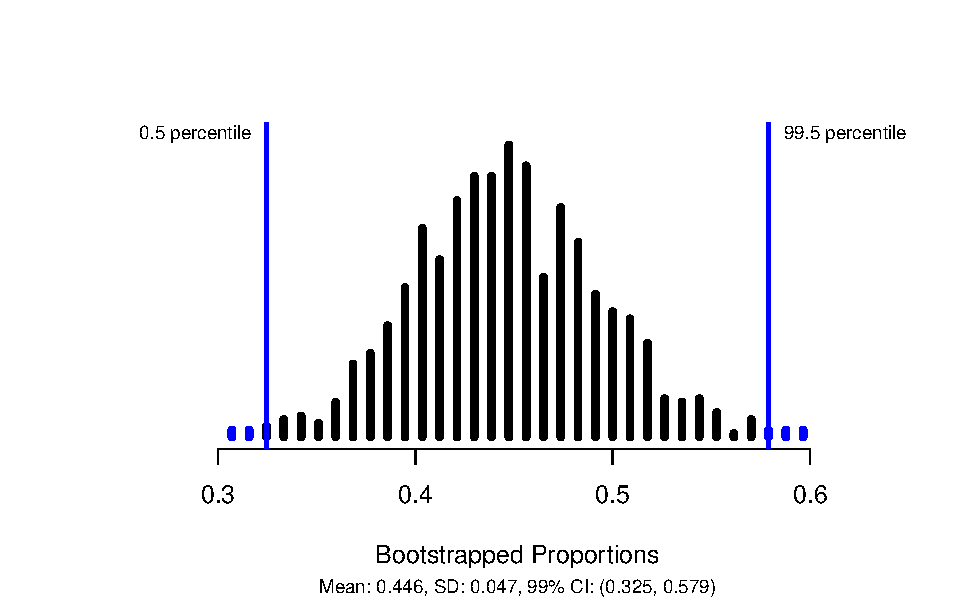
\includegraphics[width=0.7\linewidth]{06-LN06-1cat_simulation_files/figure-latex/unnamed-chunk-5-1} \end{center}
\newpage

\hypertarget{out-of-class-activity-6-helperer-hinderer-simulation-based-hypothesis-test}{%
\section{Out of Class Activity 6: Helperer-Hinderer --- Simulation-based Hypothesis Test}\label{out-of-class-activity-6-helperer-hinderer-simulation-based-hypothesis-test}}

\setstretch{1}

\hypertarget{learning-outcomes}{%
\subsection{Learning outcomes}\label{learning-outcomes}}

\begin{itemize}
\item
  Identify the two possible explanations (one assuming the null hypothesis and one assuming the alternative hypothesis) for a relationship seen in sample data.
\item
  Given a research question involving a single categorical variable, construct the null and alternative hypotheses
  in words and using appropriate statistical symbols.
\item
  Describe and perform a simulation-based hypothesis test for a single proportion.
\end{itemize}

\hypertarget{terminology-review}{%
\subsection{Terminology review}\label{terminology-review}}

In today's activity, we will introduce simulation-based hypothesis testing for a single categorical variable. Some terms covered in this activity are:

\begin{itemize}
\item
  Parameter of interest
\item
  Null hypothesis
\item
  Alternative hypothesis
\item
  Simulation
\end{itemize}

To review these concepts, see Chapters 9 \& 14 in your textbook.

\hypertarget{steps-of-the-statistical-investigation-process}{%
\subsection{Steps of the statistical investigation process}\label{steps-of-the-statistical-investigation-process}}

We will work through a five-step process to complete a hypothesis test for a single proportion, first introduced in the activity in week 1.

\begin{itemize}
\item
  \textbf{Ask a research question} that can be addressed by collecting data. What are the researchers trying to show?
\item
  \textbf{Design a study and collect data}. This step involves selecting the people or objects to be studied and how to gather relevant data on them.
\item
  \textbf{Summarize and visualize the data}. Calculate summary statistics and create graphical plots that best represent the research question.
\item
  \textbf{Use statistical analysis methods to draw inferences from the data}. Choose a statistical inference method appropriate for the data and identify the p-value and/or confidence interval after checking assumptions. In this study, we will focus on using randomization to generate a simulated p-value.
\item
  \textbf{Communicate the results and answer the research question}. Using the p-value and confidence interval from the analysis, determine whether the data provide statistical evidence against the null hypothesis. Write a conclusion that addresses the research question.
\end{itemize}

\newpage

\hypertarget{helper-hinderer}{%
\subsection{Helper-Hinderer}\label{helper-hinderer}}

A study by Hamblin, Wynn, and Bloom reported in Nature (Hamblin, Wynn, and Bloom 2007) was intended to check young kids' feelings about helpful and non-helpful behavior. Non-verbal infants ages 6 to 10 months were shown short videos with different shapes either helping or hindering the climber. As a class we will watch this short video to see how the experiment was run: \url{https://youtu.be/anCaGBsBOxM}. Researchers were hoping to assess: Are infants more likely to preferentially choose the helper toy over the hinderer toy? In the study, of the 16 infants age 6 to 10 months, 14 chose the \emph{helper} toy and 2 chose the \emph{hinderer} toy.

In this study, the \textbf{observational units are the infants ages 6 to 10 months}. The \textbf{variable measured on each observational unit (infant) is whether they chose the helper or the hinderer toy}. This is a categorical variable so we will be assessing the proportion of infants ages 6 to 10 months that choose the helper toy. Choosing the helper toy in this study will be considered a success.

\hypertarget{ask-a-research-question}{%
\subsubsection*{Ask a research question}\label{ask-a-research-question}}
\addcontentsline{toc}{subsubsection}{Ask a research question}

\begin{enumerate}
\def\labelenumi{\arabic{enumi}.}
\tightlist
\item
  Identify the research question for this study. What are the researchers hoping to show?
\end{enumerate}

\vspace{0.6in}

\hypertarget{design-a-study-and-collect-data}{%
\subsubsection*{Design a study and collect data}\label{design-a-study-and-collect-data}}
\addcontentsline{toc}{subsubsection}{Design a study and collect data}

Before using statistical inference methods, we must check that the cases are independent. The sample observations are independent if the outcome of one observation does not influence the outcome of another. One way this condition is met is if data come from a simple random sample of the target population.

\begin{enumerate}
\def\labelenumi{\arabic{enumi}.}
\setcounter{enumi}{1}
\tightlist
\item
  Are the cases independent? Justify your answer.
\end{enumerate}

\vspace{0.8in}

\hypertarget{summarize-and-visualize-the-data}{%
\subsubsection*{Summarize and visualize the data}\label{summarize-and-visualize-the-data}}
\addcontentsline{toc}{subsubsection}{Summarize and visualize the data}

The following code reads in the data set and gives the number of infants in each level of the variable, whether the infant chose the helper or the hinderer. Remember to visually display this data we can use either a frequency bar plot or a relative frequency bar plot.

\begin{Shaded}
\begin{Highlighting}[]
 \CommentTok{\# Read in data set}
\NormalTok{infants }\OtherTok{\textless{}{-}} \FunctionTok{read.csv}\NormalTok{(}\StringTok{"https://math.montana.edu/courses/s216/data/infantchoice.csv"}\NormalTok{)}
\NormalTok{infants }\SpecialCharTok{\%\textgreater{}\%} \FunctionTok{count}\NormalTok{(choice)  }\CommentTok{\# Count number in each choice category}
\end{Highlighting}
\end{Shaded}

\begin{verbatim}
#>     choice  n
#> 1   helper 14
#> 2 hinderer  2
\end{verbatim}

\[\hat{p} = \frac{\mbox{number of successes}}{\mbox{total number of observational units}}\]
\newpage

\begin{enumerate}
\def\labelenumi{\arabic{enumi}.}
\setcounter{enumi}{2}
\tightlist
\item
  Using the \texttt{R} output and the formula given, calculate the summary statistic (sample proportion) to represent the research question. Recall that \texttt{choosing\ the\ helper\ toy} is a considered a success. Use appropriate notation.
\end{enumerate}

\vspace{0.5in}

\begin{enumerate}
\def\labelenumi{\arabic{enumi}.}
\setcounter{enumi}{3}
\tightlist
\item
  Sketch a relative frequency bar plot of these data.
\end{enumerate}

\vspace{1.5in}

We cannot assess whether infants are more likely to choose the helper toy based on the statistic and plot alone. The next step is to analyze the data by using a hypothesis test to discover if there is evidence against the null hypothesis.

\hypertarget{use-statistical-analysis-methods-to-draw-inferences-from-the-data}{%
\subsubsection*{Use statistical analysis methods to draw inferences from the data}\label{use-statistical-analysis-methods-to-draw-inferences-from-the-data}}
\addcontentsline{toc}{subsubsection}{Use statistical analysis methods to draw inferences from the data}

When performing a hypothesis test, we must first identify the null hypothesis. The null hypothesis is written about the parameter of interest, or the value that summarizes the variable in the population.

For this study, the parameter of interest is the \textbf{true or population proportion of infants ages 6--10 months who will choose the helper toy}.

If the children are just randomly choosing the toy, we would expect half (0.5) of the infants to choose the helper toy. This is the null value for our study.

\begin{enumerate}
\def\labelenumi{\arabic{enumi}.}
\setcounter{enumi}{4}
\tightlist
\item
  Using the parameter of interest given above, write out the null hypothesis in words. That is, what do we assume to be true about the parameter of interest when we perform our simulation?
  \vspace{0.8in}
\end{enumerate}

The notation used for a population proportion (or probability, or true proportion) is \(\pi\). Since this summarizes a population, it is a parameter. When writing the \textbf{null hypothesis} in notation, we set the parameter equal to the null value, \(H_0: \pi = \pi_0\).

\newpage

\begin{enumerate}
\def\labelenumi{\arabic{enumi}.}
\setcounter{enumi}{5}
\tightlist
\item
  Write the null hypothesis in notation using the null value of 0.5 in place of \(\pi_0\) in the equation given on the previous page.
\end{enumerate}

\vspace{0.5in}

The \textbf{alternative hypothesis} is the claim to be tested and the direction of the claim (less than, greater than, or not equal to) is based on the research question.

\begin{enumerate}
\def\labelenumi{\arabic{enumi}.}
\setcounter{enumi}{6}
\tightlist
\item
  Based on the research question from question 1, are we testing that the parameter is greater than 0.5, less than 0.5 or different than 0.5?
\end{enumerate}

\vspace{0.4in}

\vspace{1in}

\begin{enumerate}
\def\labelenumi{\arabic{enumi}.}
\setcounter{enumi}{7}
\tightlist
\item
  Write out the alternative hypothesis in notation.
\end{enumerate}

\vspace{0.5in}

Remember that when utilizing a hypothesis test, we are evaluating two competing possibilities. For this study the \textbf{two possibilities} are either\ldots{}

\begin{itemize}
\item
  The true proportion of infants who choose the helper is 0.5 and our results just occurred by random chance; or,
\item
  The true proportion of infants who choose the helper is greater than 0.5 and our results reflect this.
\end{itemize}

Notice that these two competing possibilities represent the null and alternative hypotheses.

We will now simulate a one sample of a \textbf{null distribution} of sample proportions. The null distribution is created under the assumption the null hypothesis is true. In this case, we assume the true proportion of infants who choose the helper is 0.5, so we will create 1000 (or more) different simulations of 16 infants under this assumption.

Let's think about how to use a coin to create one simulation of 16 infants under the assumption the null hypothesis is true. Let heads equal infant chose the helper toy and tails equal infant chose the hinderer toy.

\begin{enumerate}
\def\labelenumi{\arabic{enumi}.}
\setcounter{enumi}{8}
\tightlist
\item
  How many times would you flip a coin to simulate the sample of infants?
\end{enumerate}

\vspace{0.2in}

\begin{enumerate}
\def\labelenumi{\arabic{enumi}.}
\setcounter{enumi}{9}
\tightlist
\item
  Flip a coin 16 times recording the number of times the coin lands on heads. This represents one simulated sample of 16 infants randomly choosing the toy.
\end{enumerate}

\vspace{0.2in}

\begin{enumerate}
\def\labelenumi{\arabic{enumi}.}
\setcounter{enumi}{10}
\tightlist
\item
  Is the value from question 10 closer to 0.5, the null value, or closer to the sample proportion, 0.875?
\end{enumerate}

\vspace{0.2in}

\begin{enumerate}
\def\labelenumi{\arabic{enumi}.}
\setcounter{enumi}{11}
\tightlist
\item
  Report your simulated sample proportion to your instructor via the Google sheet provided on D2L. Sketch the distribution created by your class below.
\end{enumerate}

\vspace{1.5in}

\begin{enumerate}
\def\labelenumi{\arabic{enumi}.}
\setcounter{enumi}{12}
\tightlist
\item
  Circle the observed statistic (value from question 3) on the distribution you drew in question 15. Where does this statistic fall in this distribution: Is it near the center of the distribution (near 0.5) or in one of the tails of the distribution?
\end{enumerate}

\vspace{1in}

In the next class, we will continue to assess the strength of evidence against the null hypothesis by using a computer to simulate 1000 samples when we assume the null hypothesis is true.

\hypertarget{take-home-messages}{%
\subsection{Take-home messages}\label{take-home-messages}}

\begin{enumerate}
\def\labelenumi{\arabic{enumi}.}
\item
  In a hypothesis test we have two competing hypotheses, the null hypothesis and the alternative hypothesis. The null hypothesis represents either a skeptical perspective or a perspective of no difference or no effect. The alternative hypothesis represents a new perspective such as the possibility that there has been a change or that there is a treatment effect in an experiment.
\item
  In a simulation-based test, we create a distribution of possible simulated statistics for our sample if the null hypothesis is true. Then we see if the calculated observed statistic from the data is likely or unlikely to occur when compared to the null distribution.
\item
  To create one simulated sample on the null distribution for a sample proportion, spin a spinner with probability equal to \(\pi_0\) (the null value), \(n\) times or draw with replacement \(n\) times from a deck of cards created to reflect \(\pi_0\) as the probability of success. Calculate and plot the proportion of successes from the simulated sample.
\end{enumerate}

\hypertarget{additional-notes}{%
\subsection{Additional notes}\label{additional-notes}}

Use this space to summarize your thoughts and take additional notes on today's activity and material covered.

\newpage

\hypertarget{activity-6-helper-hinderer-continued}{%
\section{Activity 6: Helper-Hinderer (continued)}\label{activity-6-helper-hinderer-continued}}

\setstretch{1}

\hypertarget{learning-outcomes-1}{%
\subsection{Learning outcomes}\label{learning-outcomes-1}}

\begin{itemize}
\item
  Describe and perform a simulation-based hypothesis test for a single proportion.
\item
  Interpret and evaluate a p-value for a simulation-based hypothesis test for a single proportion.
\item
  Explore what a p-value represents
\end{itemize}

\hypertarget{steps-of-the-statistical-investigation-process-1}{%
\subsection{Steps of the statistical investigation process}\label{steps-of-the-statistical-investigation-process-1}}

In today's activity we will continue with steps 4 and 5 in the statistical investigation process. We will continue to assess the Helper-Hinderer study from last class.

\begin{itemize}
\item
  \textbf{Ask a research question} that can be addressed by collecting data. What are the researchers trying to show?
\item
  \textbf{Design a study and collect data}. This step involves selecting the people or objects to be studied and how to gather relevant data on them.
\item
  \textbf{Summarize and visualize the data}. Calculate summary statistics and create graphical plots that best represent the research question.
\item
  \textbf{Use statistical analysis methods to draw inferences from the data}. Choose a statistical inference method appropriate for the data and identify the p-value and/or confidence interval after checking assumptions. In this study, we will focus on using randomization to generate a simulated p-value.
\item
  \textbf{Communicate the results and answer the research question}. Using the p-value and confidence interval from the analysis, determine whether the data provide statistical evidence against the null hypothesis. Write a conclusion that addresses the research question.
\end{itemize}

\hypertarget{helper-hinderer-1}{%
\subsection{Helper-Hinderer}\label{helper-hinderer-1}}

A study by Hamblin, Wynn, and Bloom reported in Nature (Hamblin, Wynn, and Bloom 2007) was intended to check young kids' feelings about helpful and non-helpful behavior. Non-verbal infants ages 6 to 10 months were shown short videos with different shapes either helping or hindering the climber. As a class we will watch this short video to see how the experiment was run: \url{https://youtu.be/anCaGBsBOxM}. Researchers were hoping to assess: Are infants more likely to preferentially choose the helper toy over the hinderer toy? In the study, of the 16 infants age 6 to 10 months, 14 chose the \emph{helper} toy and 2 chose the \emph{hinderer} toy.

\begin{enumerate}
\def\labelenumi{\arabic{enumi}.}
\tightlist
\item
  Report the sample proportion calculated in the out of class activity.
\end{enumerate}

\newpage

\begin{enumerate}
\def\labelenumi{\arabic{enumi}.}
\setcounter{enumi}{1}
\tightlist
\item
  Write the alternative hypothesis in words in context of the problem. Remember the direction we are testing is dependent on the research question.
\end{enumerate}

\vspace{0.8in}

Today, we will use the computer to simulate a null distribution of 1000 different samples of 16 infants, plotting the proportion who chose the helper in each sample, based on the assumption that the true proportion of infants who choose the helper is 0.5 (or that the null hypothesis is true).

To use the computer simulation, we will need to enter the

\begin{itemize}
\tightlist
\item
  assumed ``probability of success'' (\(\pi_0\)),
\item
  ``sample size'' (the number of observational units or cases in the sample),
\item
  ``number of repetitions'' (the number of samples to be generated),
\item
  ``as extreme as'' (the observed statistic), and
\item
  the ``direction'' (matches the direction of the alternative hypothesis).
\end{itemize}

\begin{enumerate}
\def\labelenumi{\arabic{enumi}.}
\setcounter{enumi}{2}
\tightlist
\item
  What values should be entered for each of the following into the one proportion test to create 1000 simulations?
\end{enumerate}

\vspace{1mm}

\begin{itemize}
\tightlist
\item
  Probability of success:
\end{itemize}

\vspace{.2in}

\begin{itemize}
\tightlist
\item
  Sample size:
\end{itemize}

\vspace{.2in}

\begin{itemize}
\tightlist
\item
  Number of repetitions:
\end{itemize}

\vspace{.2in}

\begin{itemize}
\tightlist
\item
  As extreme as:
\end{itemize}

\vspace{.2in}

\begin{itemize}
\tightlist
\item
  Direction (\texttt{"greater"}, \texttt{"less"}, or \texttt{"two-sided"}):
\end{itemize}

\newpage

We will use the \texttt{one\_proportion\_test()} function in \texttt{R} (in the \texttt{catstats} package) to simulate the null distribution of sample proportions and compute a p-value. Using the provided \texttt{R} script file, fill in the values/words for each \texttt{xx} with your answers from question 3 in the one proportion test to create a null distribution with 1000 simulations. Then highlight and run lines 1--15.

\begin{Shaded}
\begin{Highlighting}[]
\FunctionTok{one\_proportion\_test}\NormalTok{(}\AttributeTok{probability\_success =}\NormalTok{ xx, }\CommentTok{\# Null hypothesis value}
          \AttributeTok{sample\_size =}\NormalTok{ xx, }\CommentTok{\# Enter sample size}
          \AttributeTok{number\_repetitions =} \DecValTok{1000}\NormalTok{, }\CommentTok{\# Enter number of simulations}
          \AttributeTok{as\_extreme\_as =}\NormalTok{ xx, }\CommentTok{\# Observed statistic}
          \AttributeTok{direction =} \StringTok{"xx"}\NormalTok{, }\CommentTok{\# Specify direction of alternative hypothesis}
          \AttributeTok{summary\_measure =} \StringTok{"proportion"}\NormalTok{) }\CommentTok{\# Reporting proportion or number of successes?}
\end{Highlighting}
\end{Shaded}

\begin{enumerate}
\def\labelenumi{\arabic{enumi}.}
\setcounter{enumi}{3}
\tightlist
\item
  Sketch the null distribution created from the \texttt{R} code here.
\end{enumerate}

\vspace{1.8in}

\begin{enumerate}
\def\labelenumi{\arabic{enumi}.}
\setcounter{enumi}{4}
\tightlist
\item
  Around what value is the null distribution centered? Why does that make sense?
\end{enumerate}

\vspace{1in}

\begin{enumerate}
\def\labelenumi{\arabic{enumi}.}
\setcounter{enumi}{5}
\tightlist
\item
  Circle the observed statistic (value from question 1) on the distribution you drew in question 4. Where does this statistic fall in the null distribution: Is it near the center of the distribution (near 0.5) or in one of the tails of the distribution?
\end{enumerate}

\vspace{1in}

\begin{enumerate}
\def\labelenumi{\arabic{enumi}.}
\setcounter{enumi}{6}
\tightlist
\item
  Is the observed statistic likely to happen or unlikely to happen if the true proportion of infants who choose the helper is 0.5? Explain your answer using the plot.
\end{enumerate}

\newpage

\begin{enumerate}
\def\labelenumi{\arabic{enumi}.}
\setcounter{enumi}{7}
\tightlist
\item
  Using the simulation, what is the proportion of simulated samples that generated a sample proportion at the observed statistic or greater, if the true proportion of infants who choose the helper is 0.5? \emph{Hint}: Look under the simulation.
\end{enumerate}

\vspace{1in}

The value in question 8 is the \textbf{p-value}. The smaller the p-value, the more evidence we have against the null hypothesis.

\begin{enumerate}
\def\labelenumi{\arabic{enumi}.}
\setcounter{enumi}{8}
\tightlist
\item
  \textbf{Using the following guidelines for the strength of evidence, how much evidence do the data provide against the null hypothesis? (Circle one of the five descriptions.)}
\end{enumerate}

\begin{center}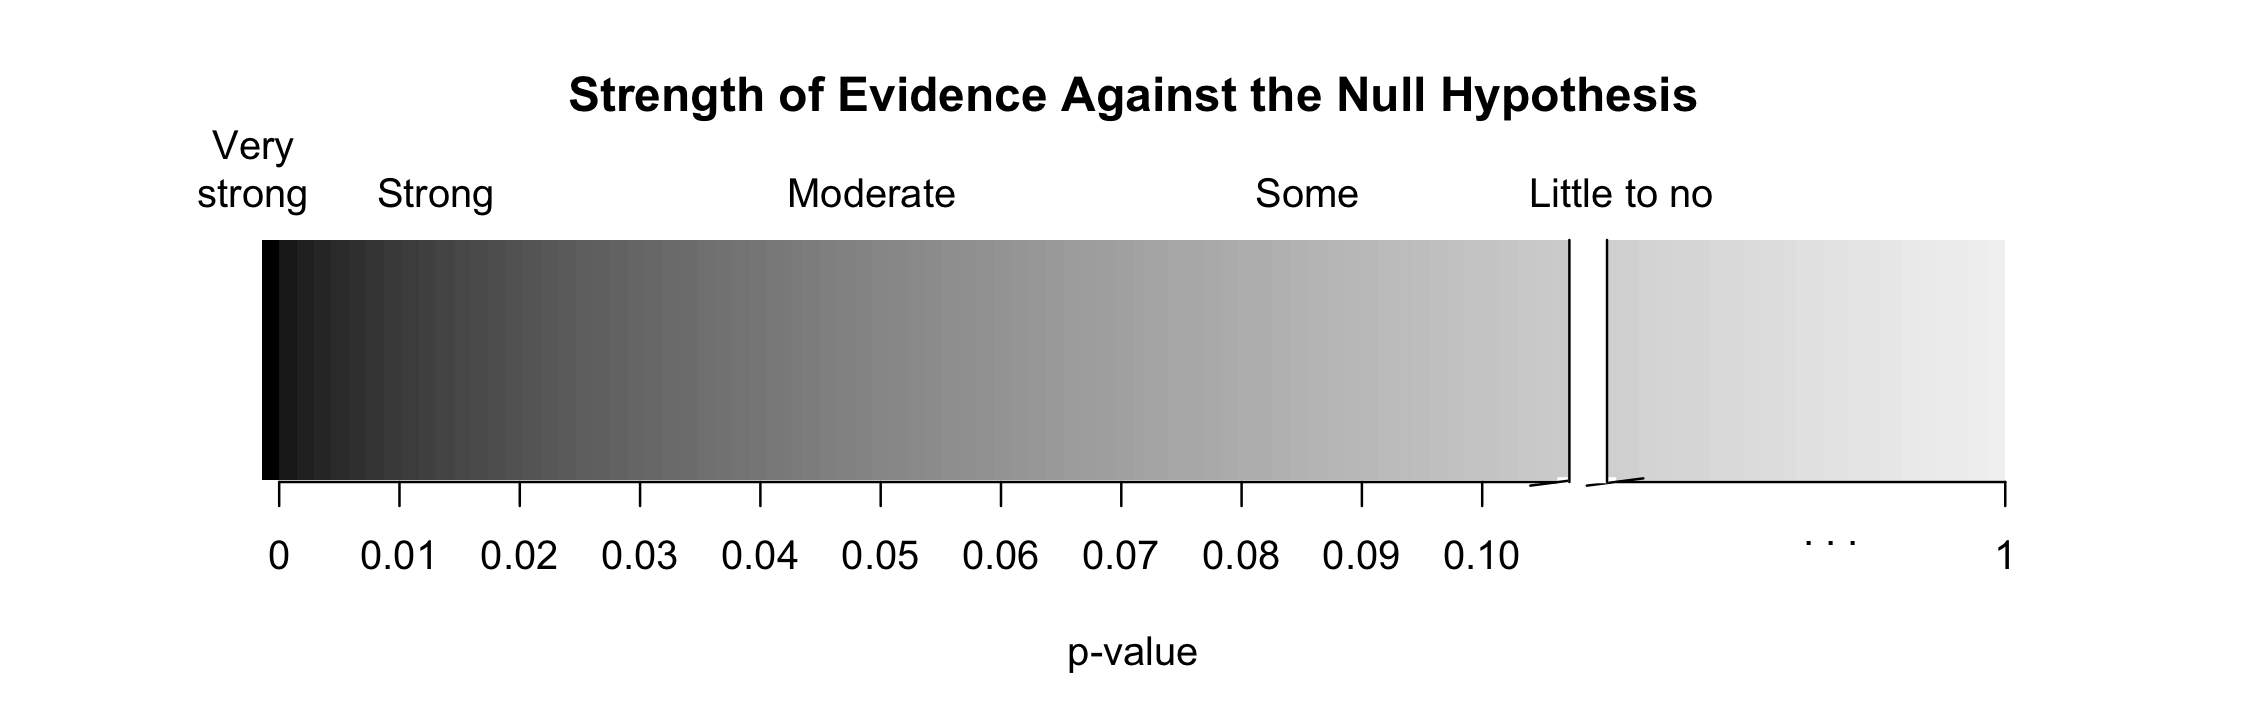
\includegraphics[width=0.9\linewidth]{images/soe_gradient_gray} \end{center}

\hypertarget{interpret-the-p-value}{%
\subsubsection*{Interpret the p-value}\label{interpret-the-p-value}}
\addcontentsline{toc}{subsubsection}{Interpret the p-value}

The p-value measures the probability that we observe a sample proportion as extreme as what was seen in the data or more extreme (matching the direction of the Ha) IF the null hypothesis is true.

\begin{enumerate}
\def\labelenumi{\arabic{enumi}.}
\setcounter{enumi}{9}
\tightlist
\item
  What did we assume to create the null distribution?
\end{enumerate}

\vspace{1in}

\begin{enumerate}
\def\labelenumi{\arabic{enumi}.}
\setcounter{enumi}{10}
\tightlist
\item
  What value did we compare to the null distribution to find the p-value?
\end{enumerate}

\vspace{0.3in}

\begin{enumerate}
\def\labelenumi{\arabic{enumi}.}
\setcounter{enumi}{11}
\tightlist
\item
  What direction did we count simulations from the statistic?
  \vspace{0.3in}
\end{enumerate}

\newpage

\begin{enumerate}
\def\labelenumi{\arabic{enumi}.}
\setcounter{enumi}{12}
\tightlist
\item
  Fill in the blanks below to interpret the p-value.
\end{enumerate}

\setstretch{1.5}

We would observe a sample proportion of (value of the sample proportion )\hrulefill  

or (greater, less, more extreme) \hrulefill   

with a probability of (value of p-value) \hrulefill  

IF we assume (\(H_0\) in context) \hrulefill.

\setstretch{1}
\vspace{12pt}

\hypertarget{communicate-the-results-and-answer-the-research-question}{%
\subsubsection*{Communicate the results and answer the research question}\label{communicate-the-results-and-answer-the-research-question}}
\addcontentsline{toc}{subsubsection}{Communicate the results and answer the research question}

When we write a conclusion we answer the research question by stating how much evidence there is for the alternative hypothesis.

\begin{enumerate}
\def\labelenumi{\arabic{enumi}.}
\setcounter{enumi}{13}
\tightlist
\item
  Write a conclusion in context of the study. How much evidence does the data provide in support of the alternative hypothesis?
\end{enumerate}

\vspace{1in}

\hypertarget{take-home-messages-1}{%
\subsection{Take-home messages}\label{take-home-messages-1}}

\begin{enumerate}
\def\labelenumi{\arabic{enumi}.}
\item
  The null distribution is created based on the assumption the null hypothesis is true. We compare the sample statistic to the distribution to find the likelihood of observing this statistic.
\item
  The p-value measures the probability of observing the sample statistic or more extreme (in direction of the alternative hypothesis) is the null hypothesis is true.
\end{enumerate}

\hypertarget{additional-notes-1}{%
\subsection{Additional notes}\label{additional-notes-1}}

Use this space to summarize your thoughts and take additional notes on today's activity and material covered.

\newpage

\hypertarget{week-6-lab-helper-hinderer-simulation-based-confidence-interval}{%
\section{Week 6 Lab: Helper-Hinderer --- Simulation-based Confidence Interval}\label{week-6-lab-helper-hinderer-simulation-based-confidence-interval}}

\setstretch{1}

\hypertarget{learning-outcomes-2}{%
\subsection{Learning outcomes}\label{learning-outcomes-2}}

\begin{itemize}
\item
  Use bootstrapping to find a confidence interval for a single proportion.
\item
  Interpret a confidence interval for a single proportion.
\end{itemize}

\hypertarget{terminology-review-1}{%
\subsection{Terminology review}\label{terminology-review-1}}

In today's activity, we will introduce simulation-based confidence intervals for a single proportion. Some terms covered in this activity are:

\begin{itemize}
\item
  Parameter of interest
\item
  Bootstrapping
\item
  Confidence interval
\end{itemize}

To review these concepts, see Chapters 10 \& 14 in your textbook.

\hypertarget{helper-hinderer-2}{%
\subsection{Helper-Hinderer}\label{helper-hinderer-2}}

In the last class, we found very strong evidence that the true proportion of infants who will choose the helper character is greater than 0.5. But what \emph{is} the true proportion of infants who will choose the helper character? We will use this same study to estimate this parameter of interest by creating a confidence interval.

As a reminder: Do young children know the difference between helpful and unhelpful behavior? A study by Hamblin, Wynn, and Bloom reported in Nature (Hamblin, Wynn, and Bloom 2007) was intended to check young kids' feelings about helpful and non-helpful behavior. Non-verbal infants ages 6 to 10 months were shown short videos with different shapes either helping or hindering the climber. Researchers were hoping to assess: Are infants more likely to preferentially choose the helper toy over the hinderer toy? In the study, of the 16 infants age 6 to 10 months, 14 chose the \emph{helper} toy and 2 chose the \emph{hinderer} toy.

A \textbf{point estimate} (our observed statistic) provides a single plausible value for a parameter. However, a point estimate is rarely perfect; usually there is some error in the estimate. In addition to supplying a point estimate of a parameter, a next logical step would be to provide a plausible \emph{range} of values for the parameter. This plausible range of values for the population parameter is called an \textbf{interval estimate} or \textbf{confidence interval}.

\hypertarget{activity-intro}{%
\subsubsection*{Activity intro}\label{activity-intro}}
\addcontentsline{toc}{subsubsection}{Activity intro}

\begin{enumerate}
\def\labelenumi{\arabic{enumi}.}
\tightlist
\item
  What is the value of the point estimate?
\end{enumerate}

\vspace{0.3in}

\begin{enumerate}
\def\labelenumi{\arabic{enumi}.}
\setcounter{enumi}{1}
\tightlist
\item
  If we took another random sample of 16 infants, would we get the exact same point estimate? Explain why or why not.
\end{enumerate}

\vspace{0.5in}

In today's activity, we will use bootstrapping to find a 95\% confidence interval for \(\pi\), the parameter of interest.

\begin{enumerate}
\def\labelenumi{\arabic{enumi}.}
\setcounter{enumi}{2}
\tightlist
\item
  In your own words, explain the bootstrapping process.
  \vspace{0.5in}
\end{enumerate}

\hypertarget{use-statistical-analysis-methods-to-draw-inferences-from-the-data-1}{%
\subsubsection*{Use statistical analysis methods to draw inferences from the data}\label{use-statistical-analysis-methods-to-draw-inferences-from-the-data-1}}
\addcontentsline{toc}{subsubsection}{Use statistical analysis methods to draw inferences from the data}

\begin{enumerate}
\def\labelenumi{\arabic{enumi}.}
\setcounter{enumi}{3}
\tightlist
\item
  Write out the parameter of interest for this study in words. \emph{Hint: this is the same as in Activity 6A.}
\end{enumerate}

\vspace{0.5in}

To use the computer simulation to create a bootstrap distribution, we will need to enter the

\begin{itemize}
\tightlist
\item
  ``sample size'' (the number of observational units or cases in the sample),
\item
  ``number of successes'' (the number of cases that choose the helper character),
\item
  ``number of repetitions'' (the number of samples to be generated), and
\item
  the ``confidence level'' (which level of confidence are we using to create the confidence interval).
\end{itemize}

\begin{enumerate}
\def\labelenumi{\arabic{enumi}.}
\setcounter{enumi}{4}
\tightlist
\item
  What values should be entered for each of the following into the simulation to create the bootstrap distribution of sample proportions to find a 95\% confidence interval?
  \vspace{1mm}
\end{enumerate}

\begin{itemize}
\tightlist
\item
  Sample size:
\end{itemize}

\vspace{.1in}

\begin{itemize}
\tightlist
\item
  Number of successes:
\end{itemize}

\vspace{.1in}

\begin{itemize}
\tightlist
\item
  Number of repetitions:
\end{itemize}

\vspace{.1in}

\begin{itemize}
\tightlist
\item
  Confidence level (as a decimal):
\end{itemize}

\vspace{.1in}

We will use the \texttt{one\_proportion\_bootstrap\_CI()} function in R (in the \texttt{catstats} package) to simulate the bootstrap distribution of sample proportions and calculate a confidence interval. Using the provided R script file, fill in the values/words for each \texttt{xx} with your answers from question 5 in the one proportion bootstrap confidence interval (CI) code to create a bootstrap distribution with 1000 simulations. Then highlight and run lines 1--7.

\begin{Shaded}
\begin{Highlighting}[]
\FunctionTok{one\_proportion\_bootstrap\_CI}\NormalTok{(}\AttributeTok{sample\_size =}\NormalTok{ xx, }\CommentTok{\# Sample size}
                    \AttributeTok{number\_successes =}\NormalTok{ xx, }\CommentTok{\# Observed number of successes}
                    \AttributeTok{number\_repetitions =} \DecValTok{1000}\NormalTok{, }\CommentTok{\# Number of bootstrap samples to use}
                    \AttributeTok{confidence\_level =} \FloatTok{0.95}\NormalTok{) }\CommentTok{\# Confidence level as a decimal}
\end{Highlighting}
\end{Shaded}

\newpage

\begin{enumerate}
\def\labelenumi{\arabic{enumi}.}
\setcounter{enumi}{5}
\tightlist
\item
  Sketch the bootstrap distribution created below.
\end{enumerate}

\vspace{1.8in}

\begin{enumerate}
\def\labelenumi{\arabic{enumi}.}
\setcounter{enumi}{6}
\item
  What is the value at the center of this bootstrap distribution? Why does this make sense?
  \vspace{.8in}
\item
  \textbf{Explain why the two vertical lines are at the 2.5th percentile and the 97.5th percentile.}
\end{enumerate}

\vspace{.7in}

\begin{enumerate}
\def\labelenumi{\arabic{enumi}.}
\setcounter{enumi}{8}
\tightlist
\item
  Report the 95\% bootstrapped confidence interval for \(\pi\). Use interval notation: (lower value, upper value).
\end{enumerate}

\vspace{0.2in}

\begin{enumerate}
\def\labelenumi{\arabic{enumi}.}
\setcounter{enumi}{9}
\tightlist
\item
  \textbf{Interpret the 95\% confidence interval in context.}
\end{enumerate}

\vspace{.7in}

\hypertarget{communicate-the-results-and-answer-the-research-question-1}{%
\subsubsection*{Communicate the results and answer the research question}\label{communicate-the-results-and-answer-the-research-question-1}}
\addcontentsline{toc}{subsubsection}{Communicate the results and answer the research question}

\begin{enumerate}
\def\labelenumi{\arabic{enumi}.}
\setcounter{enumi}{10}
\tightlist
\item
  \textbf{Is the value 0.5 (the null value) in the 95\% confidence interval?}
\end{enumerate}

\vspace{.2in}

~~~\textbf{Explain how this indicates that the p-value provides strong evidence against the null.}

\newpage

\hypertarget{effect-of-confidence-level}{%
\subsubsection*{Effect of confidence level}\label{effect-of-confidence-level}}
\addcontentsline{toc}{subsubsection}{Effect of confidence level}

\begin{enumerate}
\def\labelenumi{\arabic{enumi}.}
\setcounter{enumi}{11}
\tightlist
\item
  Suppose instead of finding a 95\% confidence interval, we found a 90\% confidence interval. Would you expect the 90\% confidence interval to be narrower or wider? Explain your answer.
\end{enumerate}

\vspace{0.4in}

\begin{enumerate}
\def\labelenumi{\arabic{enumi}.}
\setcounter{enumi}{12}
\tightlist
\item
  The following R code produced the bootstrap distribution with 1000 simulations that follows. Circle the value that changed in the code.
\end{enumerate}

\begin{Shaded}
\begin{Highlighting}[]
\FunctionTok{one\_proportion\_bootstrap\_CI}\NormalTok{(}\AttributeTok{sample\_size =} \DecValTok{16}\NormalTok{, }\CommentTok{\# Sample size}
                    \AttributeTok{number\_successes =} \DecValTok{14}\NormalTok{, }\CommentTok{\# Observed number of successes}
                    \AttributeTok{number\_repetitions =} \DecValTok{1000}\NormalTok{, }\CommentTok{\# Number of bootstrap samples to use}
                    \AttributeTok{confidence\_level =} \FloatTok{0.90}\NormalTok{) }\CommentTok{\# Confidence level as a decimal}
\end{Highlighting}
\end{Shaded}

\begin{center}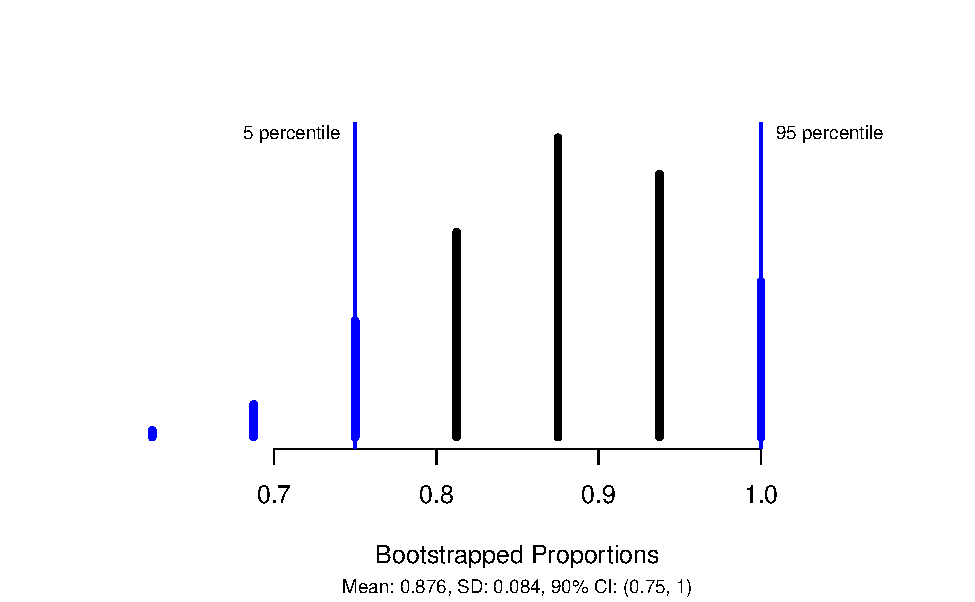
\includegraphics[width=0.7\linewidth]{06-L04-inference-1cat_CI-simulation_files/figure-latex/unnamed-chunk-2-1} \end{center}

\begin{enumerate}
\def\labelenumi{\arabic{enumi}.}
\setcounter{enumi}{13}
\tightlist
\item
  Report both the 95\% confidence interval (question 9) and the 90\% confidence interval (question 13). Is the 90\% confidence interval narrower or wider than the 95\% confidence interval?
\end{enumerate}

\vspace{0.5in}

\begin{enumerate}
\def\labelenumi{\arabic{enumi}.}
\setcounter{enumi}{14}
\tightlist
\item
  Explain why the upper value of the confidence interval is truncated at 1.
\end{enumerate}

\vspace{0.5in}

\newpage

\setstretch{1.5}

\begin{enumerate}
\def\labelenumi{\arabic{enumi}.}
\setcounter{enumi}{15}
\tightlist
\item
  Fill in the blanks below to write a paragraph summarizing the results of the study as if writing a press release. \textbf{Complete your group's paragraph on Gradescope.}\\
  Researchers were interested if infants observe social cues and would be more likely to choose the helper toy over the hinderer toy. In a sample of (sample size) \_\_\_\_\_\_\_\_\_\_\_\_\_infants, (number of successes) \_\_\_\_\_\_\_\_\_\_\_\_\_\_\_chose the helper toy. A simulation null distribution with 1000 simulations was created in RStudio. The p-value was found by calculating the proportion of simulations in the null distribution at the sample statistic of 0.875 and greater. This resulted in a p-value of (value of p-value)\_\_\_\_\_\_\_\_\_\_\_\_\_\_\_. We would observe a sample proportion of (value of the sample proportion) \_\_\_\_\_\_\_\_\_\_\_\_\_\_\_\_\_\_\_\_\_\_ or (greater, less, more extreme) \_\_\_\_\_\_\_\_\_\_\_\_\_\_\_\_\_\_\_\_\_ with a probability of (value of p-value)\_\_\_\_\_\_\_\_\_\_\_\_\_\_\_\_\_\_\_\\
  IF we assume (\(H_0\) in context) \_\_\_\_\_\_\_\_\_\_\_\_\_\_\_\_\_\_\_\_\_\_\_\_\_\_\_\_\_\_\_\_\_\_\_\_\_\_\_\_\_\_\_\_.
  Based on this p-value, there is (very strong/little to no) \_\_\_\_\_\_\_\_\_\_\_\_\_\_\_\_\_\_\_\_\_\_ evidence that the (sample/true)\_\_\_\_\_\_\_\_\_\_\_\_\_\_\_\_\_\_\_\_\_ proportion of infants age 6 to 10 months who will choose the helper toy is (greater than, less than, not equal to) \_\_\_\_\_\_\_\_\_\_\_\_\_\_\_\_\_\_\_\_\_ 0.5. In addition, a 95\% confidence interval was found for the parameter of interest. We are 95\% confident that the (true/sample)\_\_\_\_\_\_\_\_\_\_\_\_\_\_\_\_\_\_\_\_\_\_\_\_\_ proportion of infants age 6 to 10 months who will choose the helper toy is between (lower value)\_\_\_\_\_\_\_\_\_\_\_\_\_\_\_\_ and (upper value)\_\_\_\_\_\_\_\_\_\_\_\_\_\_\_\_\_\_\_\_. The results of this study can be generalized to (all infants age 6 to 10 months/infants similar to those in this study)\_\_\_\_\_\_\_\_\_\_\_\_\_\_\_\_\_\_\_\_\_\_\_\_\_\_\_ as the researchers (did/did not)\_\_\_\_\_\_\_\_\_\_\_\_\_\_\_\_\_\_\_\_\_ select a random sample.
\end{enumerate}

\setstretch{1}

\hypertarget{take-home-messages-2}{%
\subsection{Take-home messages}\label{take-home-messages-2}}

\begin{enumerate}
\def\labelenumi{\arabic{enumi}.}
\item
  The goal in a hypothesis test is to assess the strength of evidence for an effect, while the goal in creating a confidence interval is to determine how large the effect is. A \textbf{confidence interval} is a range of \emph{plausible} values for the parameter of interest.
\item
  A confidence interval is built around the point estimate or observed calculated statistic from the sample. This means that the sample statistic is always the center of the confidence interval. A confidence interval includes a measure of sample to sample variability represented by the \textbf{margin of error}.
\item
  In simulation-based methods (bootstrapping), a simulated distribution of possible sample statistics is created showing the possible sample-to-sample variability. Then we find the middle \(X\) percent of the distribution around the sample statistic using the percentile method to give the range of values for the confidence interval. This shows us that we are \(X\)\% confident that the parameter is within this range, where \(X\) represents the level of confidence.
\item
  When the null value is within the confidence interval, it is a plausible value for the parameter of interest; thus, we would find a larger p-value for a hypothesis test of that null value. Conversely, if the null value is NOT within the confidence interval, we would find a small p-value for the hypothesis test and strong evidence against this null hypothesis.
\item
  To create one simulated sample on the bootstrap distribution for a sample proportion, label \(n\) cards with the original responses. Draw with replacement \(n\) times. Calculate and plot the resampled proportion of successes.
\end{enumerate}

\hypertarget{additional-notes-2}{%
\subsection{Additional notes}\label{additional-notes-2}}

Use this space to summarize your thoughts and take additional notes on today's activity and material covered.

\newpage

\hypertarget{exam-2-review}{%
\chapter{Exam 2 Review}\label{exam-2-review}}

Use the provided data set from the Islands (ExamReviewData.csv) and the appropriate Exam 2 Review R script file to answer the following questions. Each adult (\textgreater21) islander was selected at random from all adult islanders. Variables and their descriptions are listed below. Music type (classical or heavy metal) was randomly assigned to the Islanders. Time to complete the puzzle cube was measured after listening to music for each Islander. Heart rate and blood glucose levels were both measured before and then after drinking a caffeinated beverage.

\begin{longtable}[]{@{}
  >{\raggedright\arraybackslash}p{(\columnwidth - 2\tabcolsep) * \real{0.2353}}
  >{\raggedright\arraybackslash}p{(\columnwidth - 2\tabcolsep) * \real{0.7647}}@{}}
\toprule()
\begin{minipage}[b]{\linewidth}\raggedright
\textbf{Variable}
\end{minipage} & \begin{minipage}[b]{\linewidth}\raggedright
\textbf{Description}
\end{minipage} \\
\midrule()
\endhead
\texttt{Island} & Name of Island that the Islander resides on \\
\texttt{City} & Name of City in which the Islander resides \\
\texttt{Population} & Population of the City \\
\texttt{Name} & Name of Islander \\
\texttt{Consent} & Whether the Islander consented to be in the study \\
\texttt{Gender} & Gender of Islander (M = male, F = Female) \\
\texttt{Age} & Age of Islander \\
\texttt{Married} & Marital status of Islander \\
\texttt{Smoking\_Status} & Whether the Islander is a current smoker \\
\texttt{Children} & Whether the Islander has children \\
\texttt{weight\_kg} & Weight measured in kg \\
\texttt{height\_cm} & Height measured in cm \\
\texttt{respiratory\_rate} & Breaths per minute \\
\texttt{Type\_of\_Music} & Music type (Classical or Heavy Medal) Islander was randomly assigned to listen to \\
\texttt{After\_PuzzleCube} & Time to complete puzzle cube (minutes) after listening to assigned music \\
\texttt{Education\_Level} & Highest level of education completed \\
\texttt{Balance\_Test} & Time balanced measured in seconds with eyes closed \\
\texttt{Blood\_Glucose\_before} & Level of blood glucose (mg/dL) before consuming assigned drink \\
\texttt{Heart\_Rate\_before} & Heart rate (bpm) before consuming assigned drink \\
\texttt{Blood\_Glucose\_after} & Level of blood glucose (mg/dL) after consuming assigned drink \\
\texttt{Heart\_Rate\_after} & Heart rate (bpm) after consuming assigned drink \\
\texttt{Diff\_Heart\_Rate} & Difference in heart rate (bpm) for Before - After consuming assigned drink \\
\texttt{Diff\_Blood\_Glucose} & Difference in blood glucose (mg/dL) for Before - After consuming assigned drink \\
\bottomrule()
\end{longtable}

\newpage

\begin{enumerate}
\def\labelenumi{\arabic{enumi}.}
\tightlist
\item
  Use the appropriate Exam 2 Review R script file and analyze the following research question: The proportion of university graduates in the US is 42\%. ``Is there evidence that the proportion of university graduates in the Islands differs from the proportion in the US?''
\end{enumerate}

\begin{enumerate}
\def\labelenumi{\alph{enumi}.}
\item
  Parameter of Interest:
  \vspace{0.3in}
\item
  Null Hypothesis:

  Notation:
  \vspace{0.3in}

  Words:
  \vspace{0.5in}
\item
  Alternative Hypothesis:

  Notation:
  \vspace{0.3in}

  Words:
  \vspace{0.5in}
\item
  Use the R script file to get the counts for each level of the variable. Fill in the following table with the success, failure, variable name, and counts using the values from the R output.
\end{enumerate}

\begingroup
\begin{center}
\setlength{\tabcolsep}{14pt} 
\renewcommand{\arraystretch}{2} 
\begin{tabular}{|p{2in}|p{2in}|}
\hline
 {\textbf{Variable}} & {\textbf{Counts}} \\ 
 & \\ \hline
 Success & \\ 
 &  \\ \hline
 Failure & \\ 
 &  \\ \hline
 Total &  \\ 
 & \\ \hline  
\end{tabular}
\end{center}
\endgroup

\begin{enumerate}
\def\labelenumi{\alph{enumi}.}
\setcounter{enumi}{4}
\item
  Calculate the value of summary statistic to answer the research question. Give appropriate notation.
  \vspace{0.3in}
\item
  Interpret the value of the summary statistic in context of the problem:
  \vspace{0.3in}
\item
  Assess if the following conditions are met:

  Independence (needed for both simulation and theory-based methods):
  \vspace{0.8in}

  Success-Failure (must be met to use theory-based methods):
  \vspace{0.8in}
\item
  Use the provided R script file to find the simulation p-value to assess the research question. Report the p-value.
  \vspace{0.3in}
\item
  Interpret the p-value in the context of the problem.
  \vspace{0.8in}
\item
  Write a conclusion to the research question based on the p-value.
  \vspace{0.8in}
\item
  Write a decision based on the p-value.
  \vspace{0.3in}
\item
  Use the provided R script file to find a 90\% confidence interval.
  \vspace{0.3in}
\item
  Interpret the 90\% confidence interval in context of the problem.
  \vspace{0.8in}
\item
  Regardless to your answer in part g, calculate the standardized statistic.
  \vspace{0.4in}
\item
  Interpret the value of the standardized statistic in context of the problem.
  \vspace{0.8in}
\item
  Use the provided R script file to find the theory-based p-value.
  \vspace{0.3in}
\item
  Use the provided R script file to find the appropriate z* multiplier and calculate the theory-based confidence interval.
  \vspace{0.5in}
\item
  Does the theory-based p-value and CI match those found using simulation methods? Explain why or why not.
  \vspace{0.8in}
\item
  To what group can the results be generalized?
  \vspace{0.8in}
\end{enumerate}

\begin{enumerate}
\def\labelenumi{\arabic{enumi}.}
\setcounter{enumi}{1}
\tightlist
\item
  Use the appropriate Exam 2 Review R script file and analyze the following research question: ``Is there evidence that those with a higher education level are less likely to smoke?''
\end{enumerate}

\begin{enumerate}
\def\labelenumi{\alph{enumi}.}
\item
  Parameter of Interest:
  \vspace{0.3in}
\item
  Null Hypothesis:

  Notation:
  \vspace{0.3in}

  Words:
  \vspace{0.5in}
\item
  Alternative Hypothesis:

  Notation:
  \vspace{0.3in}

  Words:
  \vspace{0.5in}
\item
  Use the R script file to get the counts for each level and combination of variables. Fill in the following table with the variable names, levels of each variable, and counts using the values from the R output.
\end{enumerate}

\begingroup
\setlength{\tabcolsep}{14pt}
\renewcommand{\arraystretch}{2}
\begin{center}
\begin{tabular}{|c|p{1in}|p{1in}|p{1in}|}
\hline
 & \multicolumn{2}{|c|}{\textbf{Explanatory Variable}} & \\ 
 & \multicolumn{2}{|c|}{ } & \\ \hline
\textbf{Response variable} & Group 1 & Group 2 & Total \\
 & & & \\ \hline
 Success & & & \\
 & & & \\ \hline
 Failure & & & \\
 & & & \\ \hline
 Total & & & \\
 & & & \\ \hline
\end{tabular}
\end{center}
\endgroup

\begin{enumerate}
\def\labelenumi{\alph{enumi}.}
\setcounter{enumi}{3}
\tightlist
\item
  Calculate the value of summary statistic to answer the research question. Give appropriate notation.
\end{enumerate}

\vspace{0.4in}

\begin{enumerate}
\def\labelenumi{\alph{enumi}.}
\setcounter{enumi}{4}
\tightlist
\item
  Interpret the value of the summary statistic in context of the problem:
\end{enumerate}

\vspace{0.4in}

\begin{enumerate}
\def\labelenumi{\alph{enumi}.}
\setcounter{enumi}{6}
\item
  Assess if the following conditions are met:

  Independence (needed for both simulation and theory-based methods):
  \vspace{0.8in}

  Success-Failure (must be met to use theory-based methods):
  \vspace{0.8in}
\item
  Use the provided R script file to find the simulation p-value to assess the research question. Report the p-value.
  \vspace{0.3in}
\item
  Interpret the p-value in the context of the problem.
  \vspace{0.8in}
\item
  Write a conclusion to the research question based on the p-value.
  \vspace{0.8in}
\item
  Write a decision based on the p-value.
  \vspace{0.3in}
\item
  Use the provided R script file to find a 95\% confidence interval.
  \vspace{0.3in}
\item
  Interpret the 95\% confidence interval in context of the problem.
  \vspace{0.8in}
\item
  Regardless to your answer in part g, calculate the standardized statistic.
  \vspace{0.4in}
\item
  Interpret the value of the standardized statistic in context of the problem.
  \vspace{0.8in}
\item
  Use the provided R script file to find the theory-based p-value.
  \vspace{0.3in}
\item
  Use the provided R script file to find the appropriate z* multiplier and calculate the theory-based confidence interval.
  \vspace{0.5in}
\item
  Does the theory-based p-value and CI match those found using simulation methods? Explain why or why not.
  \vspace{0.8in}
\item
  What is the scope of inference for this study?
  \vspace{0.8in}
\end{enumerate}

\newpage

\hypertarget{inference-for-a-quantitative-response-with-paired-samples}{%
\chapter{Inference for a Quantitative Response with Paired Samples}\label{inference-for-a-quantitative-response-with-paired-samples}}

\hypertarget{module-11-reading-guide-inference-for-a-single-mean-or-paired-mean-difference}{%
\section{Module 11 Reading Guide: Inference for a Single Mean or Paired Mean Difference}\label{module-11-reading-guide-inference-for-a-single-mean-or-paired-mean-difference}}

\hypertarget{chapter-17-inference-for-a-single-mean}{%
\subsection*{Chapter 17 (Inference for a single mean)}\label{chapter-17-inference-for-a-single-mean}}
\addcontentsline{toc}{subsection}{Chapter 17 (Inference for a single mean)}

\textbf{Videos}

\begin{itemize}
\tightlist
\item
  17.1
\item
  17.2
\item
  17.3Tests
\item
  17.4Intervals
\end{itemize}

\setstretch{1.25}

\hypertarget{reminders-from-previous-sections-1}{%
\subsubsection*{Reminders from previous sections}\label{reminders-from-previous-sections-1}}
\addcontentsline{toc}{subsubsection}{Reminders from previous sections}

\(n\) = sample size

\(\overline{x}\) = sample mean

\(s\) = sample standard deviation

\(\mu\) = population mean

\(\sigma\) = population standard deviation

General steps of a hypothesis test:

\begin{enumerate}
\def\labelenumi{\arabic{enumi}.}
\item
  Frame the research question in terms of hypotheses.
\item
  Collect and summarize data using a test statistic.
\item
  Assume the null hypothesis is true, and simulate or mathematically model a null distribution for the test statistic.
\item
  Compare the observed test statistic to the null distribution to calculate a p-value.
\item
  Make a conclusion based on the p-value and write the conclusion in context.
\end{enumerate}

Parameter: a value summarizing a variable(s) for a population.

Statistic: a value summarizing a variable(s) for a sample.

Sampling distribution: plot of statistics from 1000s of samples of the same size taken from the same population.

Standard deviation of a statistic: the variability of statistics from 1000s of samples; how far, on average, each statistic is from the true value of the parameter.

Standard error of a statistic: estimated standard deviation of a statistic.

Hypothesis test: a process to determine how strong the evidence of an effect is. Also called a `significance test'.

Simulation-based method: Simulate lots of samples of size \(n\) under assumption of the null hypothesis, then find the proportion of the simulations that are at least as extreme as the observed sample statistic.

Theory-based method: Develop a mathematical model for the sampling distribution of the statistic under the null hypothesis and use the model to calculate the probability of the observed sample statistic (or one more extreme) occurring.

Null hypothesis (\(H_0\)): the skeptical perspective; no difference; no change; no effect; random chance; what the researcher hopes to prove is \textbf{wrong}.

Alternative hypothesis (\(H_A\)): the new perspective; a difference/increase/decrease; an effect; not random chance; what the researcher hopes to prove is \textbf{correct}.

Null value: the value of the parameter when we assume the null hypothesis is true (labeled as \(parameter_0\)).

Null distribution: the simulated or modeled distribution of statistics (sampling distribution) we would expect to occur if the null hypothesis is true.

P-value: probability of seeing the observed sample data, or something more extreme, assuming the null hypothesis is true.

\(\implies\) Lower the p-value the stronger the evidence AGAINST the null hypothesis and FOR the alternative hypothesis.

Decision: a determination of whether to reject or fail to reject a null hypothesis based on a p-value and a pre-set level of significance.

\begin{itemize}
\item
  If p-value \(\leq \alpha\), then reject \(H_0\).
\item
  If p-value \(> \alpha\), then fail to reject \(H_0\).
\end{itemize}

Significance level (\(\alpha\)): a threshold used to determine if a p-value provides enough evidence to reject the null hypothesis or not.

\rgi Common levels of \(\alpha\) include 0.01, 0.05, and 0.10.

Statistically significant: results are considered statistically significant if the p-value is below the significance level.

Confidence interval: a process to determine how large an effect is; a range of plausible values for the parameter. Also called `estimation'.

Margin of error: the value that is added to and subtracted from the sample statistic to create a confidence interval; half the width of a confidence interval.

Bootstrapping: the process of drawing with replacement \(n\) times from the original sample.

Bootstrapped resample: a random sample of size \(n\) from the original sample, selected with replacement.

Bootstrapped statistic: the statistic recorded from the bootstrapped resample.

Confidence level: how confident we are that the confidence interval will capture the parameter.

Bootstrap \(X\)\% confidence interval: (\((\frac{(1-X)}{2})^{th}\) percentile, \((X+(\frac{(1-X)}{2})^{th}\) percentile) of a bootstrap distribution.

Central Limit Theorem: For large sample sizes, the sampling distribution of a sample mean (or proportion) will be approximately normal (bell-shaped and symmetric).

\hypertarget{vocabulary-2}{%
\subsubsection*{Vocabulary}\label{vocabulary-2}}
\addcontentsline{toc}{subsubsection}{Vocabulary}

Shifted bootstrap test:
\rgs

\(t\)-distribution:
\rgs 

\begin{itemize}
\item
  The variability in the \(t\)-distribution depends on the sample size (used to calculate degrees of freedom --- df for short).
\item
  The larger df, the closer the \(t\) distribution is to the standard normal distribution.
\end{itemize}

Degrees of freedom (df):
\rgs 

T-score:
\rgs 

\hypertarget{notes-2}{%
\subsubsection*{Notes}\label{notes-2}}
\addcontentsline{toc}{subsubsection}{Notes}

To create a shifted bootstrap distribution test,

\rgi How many cards will you need and how will the cards be labeled?
\rgs 

\rgi Why are the data values shifted prior to being written on the cards?
\rgs

\rgi What do you do with the cards after labeling them?
\rgs 

\rgi After resampling, what value will be plotted on the bootstrap distribution?
\rgs 

True or false: Bootstrapping can only be used if the sample size is small.
\rgs 

Why do we use a \(t\)-distribution rather than the normal distribution when analyzing quantitative data?
\rgs 

How do we calculate degrees of freedom for the \(t\)-distribution?
\rgs 

Conditions to use the CLT for means:

\rgi Independence:
\rgs 

\rgi \rgi Checked by:
\rgs 

\rgi Normality:
\rgs 

\rgi \rgi Checked by:
\rgs 

\hypertarget{formulas-1}{%
\subsubsection*{Formulas}\label{formulas-1}}
\addcontentsline{toc}{subsubsection}{Formulas}

\(SE(\overline{x})=\)
\rgs 

\(T=\)
\rgs 

Confidence interval for a single mean:
\rgs 

\hypertarget{notation}{%
\subsubsection*{Notation}\label{notation}}
\addcontentsline{toc}{subsubsection}{Notation}

\(\mu_0\) represents
\rgs 

\hypertarget{example-from-section-17.1-edinburgh-rentals}{%
\subsubsection*{Example from section 17.1: Edinburgh rentals}\label{example-from-section-17.1-edinburgh-rentals}}
\addcontentsline{toc}{subsubsection}{Example from section 17.1: Edinburgh rentals}

\begin{enumerate}
\def\labelenumi{\arabic{enumi}.}
\item
  What are the observational units?
  \rgs 
\item
  What are the sample statistics presented in this example? What notation would be used to represent each value?
  \rgs 
\item
  What is the parameter representing in the context of this problem? What notation would be used to represent this parameter?
  \rgs 
  \rgs 
\item
  How could we use cards to simulate \textbf{one} bootstrap resample \emph{which does not assume the null hypothesis is true}? How many cards? What is written on the cards? What would we do with the cards? What would you record once you have a simulated sample?
  \rgs 
  \rgs 
  \rgs 
\item
  After 1000 resamples are generated, where is the resulting bootstrap distribution centered? Why does that make sense?
  \rgs 
  \rgs 
\item
  Based on Figure 17.3, give the confidence interval for the true mean for each of the following confidence levels.
\end{enumerate}

\rgi 90\% confidence interval =
\rgs 

\rgi 95\% confidence interval =
\rgs 

\rgi 99\% confidence interval =
\rgs 

\begin{enumerate}
\def\labelenumi{\arabic{enumi}.}
\setcounter{enumi}{6}
\tightlist
\item
  Interpret your 99\% confidence interval in the context of the problem.
  \rgs 
  \rgs 
\end{enumerate}

\hypertarget{example-from-section-17.2-sleep-times-of-msu-students}{%
\subsubsection*{Example from section 17.2: Sleep times of MSU students}\label{example-from-section-17.2-sleep-times-of-msu-students}}
\addcontentsline{toc}{subsubsection}{Example from section 17.2: Sleep times of MSU students}

\begin{enumerate}
\def\labelenumi{\arabic{enumi}.}
\item
  What is the research question?
  \rgs
\item
  What are the observational units?
  \rgs
\item
  Can the results of this study be generalized to a larger population? Why or why not?
  \rgs
\item
  What are the sample statistics presented in this example? What notation would be used to represent each value?
  \rgs
\item
  What is the parameter representing in the context of this problem? What notation would be used to represent this parameter?
  \rgs
  \rgs
\item
  Write the null and the alternative hypotheses in words.
  \rgs
  \rgs
\item
  Write the null and the alternative hypotheses in notation.
  \rgs
\item
  How could we use cards to simulate \textbf{one} shifted bootstrap resample \emph{which assumes the null hypothesis is true}? How many cards? What is written on the cards (be sure to include the amount and direction of the shift)? What would we do with the cards? What would you record once you have a simulated sample?
  \rgs 
  \rgs 
  \rgs 
\item
  What was the p-value of the test?
  \rgs
\item
  Interpret the p-value in the context of the problem.
  \rgs
  \rgs
\item
  At the 5\% significance level, what decision would you make? What type of error might that be?
  \rgs
\item
  What conclusion should the researcher make?
  \rgs
  \rgs
\item
  Are the results in this example statistically significant? Justify your answer.
  \rgs
\end{enumerate}

\hypertarget{example-from-section-17.3-mercury-content-of-dolphin-muscle}{%
\subsubsection*{Example from section 17.3: Mercury content of dolphin muscle}\label{example-from-section-17.3-mercury-content-of-dolphin-muscle}}
\addcontentsline{toc}{subsubsection}{Example from section 17.3: Mercury content of dolphin muscle}

\begin{enumerate}
\def\labelenumi{\arabic{enumi}.}
\item
  What is the research question?
  \rgs 
\item
  What are the observational units?
  \rgs 
\item
  Can the results of this study be generalized to a larger population? Why or why not?
  \rgs 
\item
  What are the sample statistics presented in this example? What notation would be used to represent each value?
  \rgs 
\item
  What is the parameter representing in the context of this problem? What notation would be used to represent this parameter?
  \rgs 
  \rgs 
\item
  Are the independence and normality conditions satisfied?
  \rgs 
  \rgs 
\item
  Calculate the standard error of the sample mean.
  \rgs 
  \rgs
\item
  What distribution should be referenced to find the multiplier for a 95\% confidence interval?
  \rgs 
\item
  Using \(t^\star=2.10\), calculate a 95\% confidence interval for \(\mu\).
  \rgs 
  \rgs
\item
  Interpret the interval calculated in the context of the problem.
  \rgs 
  \rgs 
\end{enumerate}

\hypertarget{example-from-section-17.3-cherry-blossom-race}{%
\subsubsection*{Example from section 17.3: Cherry Blossom Race}\label{example-from-section-17.3-cherry-blossom-race}}
\addcontentsline{toc}{subsubsection}{Example from section 17.3: Cherry Blossom Race}

\begin{enumerate}
\def\labelenumi{\arabic{enumi}.}
\item
  What is the research question?
  \rgs
\item
  What are the observational units?
  \rgs
\item
  Can the results of this study be generalized to a larger population? Why or why not?
  \rgs
\item
  What are the sample statistics presented in this example? What notation would be used to represent each value?
  \rgs
\item
  What is the parameter representing in the context of this problem? What notation would be used to represent this parameter?
  \rgs
  \rgs
\item
  Are the independence and normality conditions satisfied?
  \rgs
  \rgs
\item
  Write the null and the alternative hypotheses in words.
  \rgs
  \rgs
\item
  Write the null and the alternative hypotheses in notation.
  \rgs
\item
  Calculate the standard error of the sample mean.
  \rgs
  \rgs
\item
  Calculate the T-score (the standardized statistic for the sample mean).
  \rgs
  \rgs
\item
  What distribution should the T-score be compared to in order to calculate a p-value?
  \rgs
\item
  What was the p-value of the test?
  \rgs
\item
  Interpret the p-value in the context of the problem.
  \rgs
  \rgs
\item
  At the 5\% significance level, what decision would you make? What type of error might that be?
  \rgs
\item
  What conclusion should the researcher make?
  \rgs
  \rgs
\item
  Are the results in this example statistically significant? Justify your answer.
  \rgs
\end{enumerate}

\hypertarget{chapter-18-inference-for-paired-mean-difference}{%
\subsection*{Chapter 18 (Inference for paired mean difference)}\label{chapter-18-inference-for-paired-mean-difference}}
\addcontentsline{toc}{subsection}{Chapter 18 (Inference for paired mean difference)}

\setstretch{1}

\textbf{Videos}

\begin{itemize}
\tightlist
\item
  Paired\_Data
\item
  18.1and18.2
\item
  18.3
\end{itemize}

\setstretch{1.25}

\hypertarget{vocabulary-3}{%
\subsubsection*{Vocabulary}\label{vocabulary-3}}
\addcontentsline{toc}{subsubsection}{Vocabulary}

Paired data:
\rgs

\rgi Paired with repeated measures:
\rgs

\rgi Paired with matching:
\rgs

\hypertarget{notes-3}{%
\subsubsection*{Notes}\label{notes-3}}
\addcontentsline{toc}{subsubsection}{Notes}

For each of the following scenarios, determine if the two sets of observations are paired or independent.

\begin{enumerate}
\def\labelenumi{\arabic{enumi}.}
\item
  To test whether the IQ is related to genetics, researchers measured the IQ of two biological parents and the IQ of their first-born child. The average parent IQ was compared to the IQ of the first born child.
  \rgs
\item
  Hoping to see how exercise is related to heart rates, researchers asked a group of 30 volunteers to do either bicycle kicks or jumping jacks for 30 seconds. Each volunteer's heart rate was measured at the end of 30 seconds, then the volunteer sat for a 5 minute rest period. At the end of the rest period, the volunteer performed the other activity and their heart rate was measured again. Which activity was done first was randomly assigned.
  \rgs
\item
  Researchers hoping to look into the effectiveness of blended learning gathered two random samples of 50 8th graders (one at Belgrade Middle School which had 5 full-day instruction at the time of the study, the other from Chief Joseph Middle School which utilized a 2-day on, 3-day off blended learning structure). All 8th graders were given the same lessons and same homework, then asked to take the same end-of-unit test.
  \rgs
\end{enumerate}

Conditions to use the CLT for paired mean difference:

\rgi Independence:
\rgs

\rgi \rgi Checked by:
\rgs 

\rgi Normality:
\rgs

\rgi \rgi Checked by:
\rgs

\hypertarget{formulas-2}{%
\subsubsection*{Formulas}\label{formulas-2}}
\addcontentsline{toc}{subsubsection}{Formulas}

\(SE(\overline{x_d})=\)
\rgs

\(T=\)
\rgs

Confidence interval for a paired mean difference:
\rgs

\hypertarget{notation-1}{%
\subsubsection*{Notation}\label{notation-1}}
\addcontentsline{toc}{subsubsection}{Notation}

\(\overline{x_d}=\)
\rgs

\(s_d=\)
\rgs

\(\mu_d=\)
\rgs

\(\sigma_d=\)
\rgs

\hypertarget{example-from-section-18.1-tires}{%
\subsubsection*{Example from section 18.1: Tires}\label{example-from-section-18.1-tires}}
\addcontentsline{toc}{subsubsection}{Example from section 18.1: Tires}

\begin{enumerate}
\def\labelenumi{\arabic{enumi}.}
\item
  What are the observational units?
  \rgs
\item
  Why should we treat these data as paired rather than two independent samples?
  \rgs
\item
  What are the sample statistics presented in this example? What notation would be used to represent each value?
  \rgs
\item
  What is the parameter representing in the context of this problem? What notation would be used to represent this parameter?
  \rgs
  \rgs
\item
  Write the null and alternative hypotheses in appropriate notation.
  \rgs
\item
  How could we use cards to simulate \textbf{one} shifted bootstrap resample \emph{which assumes the null hypothesis is true}? How many cards? What is written on the cards? What would we do with the cards? What would you record once you have a simulated sample?
  \rgs
  \rgs
  \rgs
\item
  After 1000 resamples are generated, where is the resulting null distribution centered? Why does that make sense?
  \rgs
\item
  What was the p-value of the test? Interpret this p-value in the context of the problem.
  \rgs
  \rgs
\item
  Write a conclusion in the context of the problem.
  \rgs
\end{enumerate}

\hypertarget{example-from-sections-18.2-and-18.3-ucla-textbook-prices}{%
\subsubsection*{Example from sections 18.2 and 18.3: UCLA textbook prices}\label{example-from-sections-18.2-and-18.3-ucla-textbook-prices}}
\addcontentsline{toc}{subsubsection}{Example from sections 18.2 and 18.3: UCLA textbook prices}

\begin{enumerate}
\def\labelenumi{\arabic{enumi}.}
\item
  What is the research question?
  \rgs
\item
  What are the observational units?
  \rgs
\item
  Why should we treat these data as paired rather than two independent samples?
  \rgs
\item
  What are the sample statistics presented in this example? What notation would be used to represent each value?
  \rgs
\item
  What is the parameter representing in the context of this problem? What notation would be used to represent this parameter?
  \rgs
  \rgs
\item
  How could we use cards to simulate \textbf{one} bootstrap resample \emph{which does not assume the null hypothesis is true}? How many cards? What is written on the cards? What would we do with the cards? What would you record once you have a simulated sample?
  \rgs
  \rgs
  \rgs
\item
  After 1000 resamples are generated, where is the resulting bootstrap distribution centered? Why does that make sense?
  \rgs
  \rgs
\item
  Give the 95\% confidence interval for \(\mu_d\).
  \rgs
\item
  Interpret your 95\% confidence interval in the context of the problem.
  \rgs
  \rgs
\item
  Are the independence and normality conditions satisfied?
  \rgs
  \rgs
\item
  Write the null and the alternative hypotheses in words.
  \rgs
  \rgs
\item
  Calculate the standard error of the sample mean difference.
  \rgs
  \rgs
\item
  Calculate the T-score (the standardized statistic for the sample mean difference).
  \rgs
  \rgs
\item
  What distribution should the T-score be compared to in order to calculate a p-value?
  \rgs
\item
  What was the p-value of the test?
  \rgs
\item
  At the 5\% significance level, what decision would you make? What type of error might that be?
  \rgs
\item
  What conclusion should the researcher make?
  \rgs
  \rgs
\item
  Are the results in this example statistically significant? Justify your answer.
  \rgs
\item
  Using \(t^\star=2.00\), calculate a 95\% confidence interval for \(\mu_d\).
  \rgs
  \rgs
\item
  Interpret the interval calculated in the context of the problem.
  \rgs
  \rgs
\end{enumerate}

\newpage

\hypertarget{lecture-notes-week-11-inference-for-a-single-mean-paired-data}{%
\section{Lecture Notes Week 11: Inference for a Single Mean \& Paired Data}\label{lecture-notes-week-11-inference-for-a-single-mean-paired-data}}

\setstretch{1}

\hypertarget{single-quantitative-variable}{%
\subsection{Single quantitative variable}\label{single-quantitative-variable}}

\begin{itemize}
\item
  Reminder: review summary measures and plots discussed in the Week 3 material and Chapter 5 of the textbook.
\item
  The summary measure for a single quantitative variable is the \_\_\_\_\_\_\_\_\_\_\_\_\_\_.
\end{itemize}

\setstretch{1.5}

Notation:

\begin{itemize}
\item
  Population mean:
\item
  Population standard deviation:
\item
  Sample mean:
\item
  Sample standard deviation:
\item
  Sample size:
\end{itemize}

\setstretch{1}

Example: What is the average weight of adult male polar bears? The weight was measured on a representative sample of 83 male polar bears from the Southern Beaufort Sea.

\begin{Shaded}
\begin{Highlighting}[]
\NormalTok{pb }\OtherTok{\textless{}{-}} \FunctionTok{read.csv}\NormalTok{(}\StringTok{"https://math.montana.edu/courses/s216/data/polarbear.csv"}\NormalTok{)}
\end{Highlighting}
\end{Shaded}

Plots of the data:

\begin{Shaded}
\begin{Highlighting}[]
\NormalTok{pb }\SpecialCharTok{\%\textgreater{}\%}
    \FunctionTok{ggplot}\NormalTok{(}\FunctionTok{aes}\NormalTok{(}\AttributeTok{x =}\NormalTok{ Weight)) }\SpecialCharTok{+}   \CommentTok{\# Name variable to plot}
    \FunctionTok{geom\_histogram}\NormalTok{(}\AttributeTok{binwidth =} \DecValTok{10}\NormalTok{) }\SpecialCharTok{+}  \CommentTok{\# Create histogram with specified binwidth }
    \FunctionTok{labs}\NormalTok{(}\AttributeTok{title =} \StringTok{"Histogram of Male Polar Bear Weight"}\NormalTok{, }\CommentTok{\# Title for plot}
       \AttributeTok{x =} \StringTok{"Weight (kg)"}\NormalTok{, }\CommentTok{\# Label for x axis}
       \AttributeTok{y =} \StringTok{"Frequency"}\NormalTok{) }\CommentTok{\# Label for y axis}

\NormalTok{pb }\SpecialCharTok{\%\textgreater{}\%} \CommentTok{\# Data set piped into...}
\FunctionTok{ggplot}\NormalTok{(}\FunctionTok{aes}\NormalTok{(}\AttributeTok{x =}\NormalTok{ Weight)) }\SpecialCharTok{+}   \CommentTok{\# Name variable to plot}
  \FunctionTok{geom\_boxplot}\NormalTok{() }\SpecialCharTok{+}  \CommentTok{\# Create boxplot }
  \FunctionTok{labs}\NormalTok{(}\AttributeTok{title =} \StringTok{"Boxplot of Male Polar Bear Weight"}\NormalTok{, }\CommentTok{\# Title for plot}
       \AttributeTok{x =} \StringTok{"Weight (kg)"}\NormalTok{, }\CommentTok{\# Label for x axis}
       \AttributeTok{y =} \StringTok{"Frequency"}\NormalTok{) }\CommentTok{\# Label for y axis}
\end{Highlighting}
\end{Shaded}

\begin{center}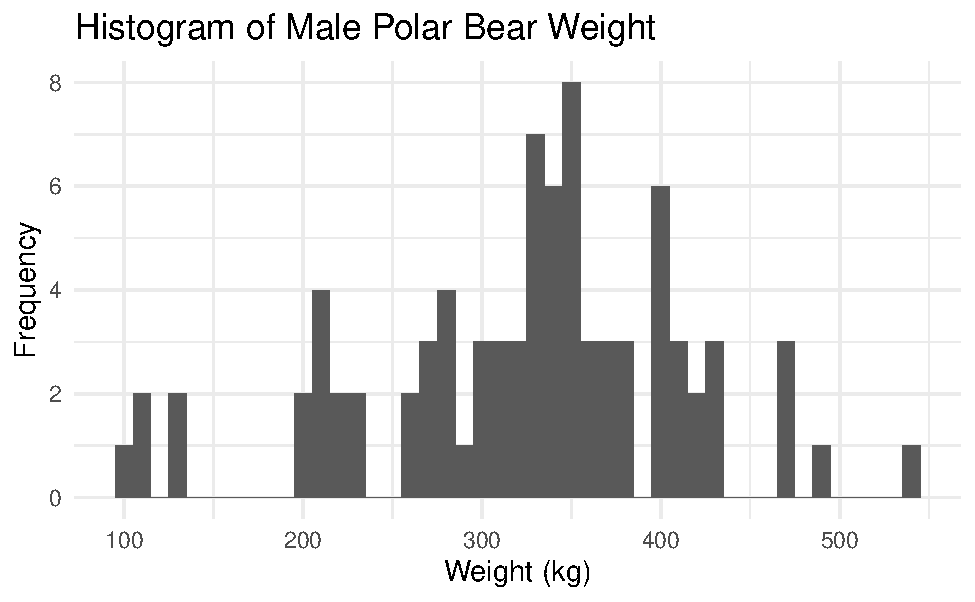
\includegraphics[width=0.6\linewidth]{11-LN011-paired_files/figure-latex/unnamed-chunk-2-1} 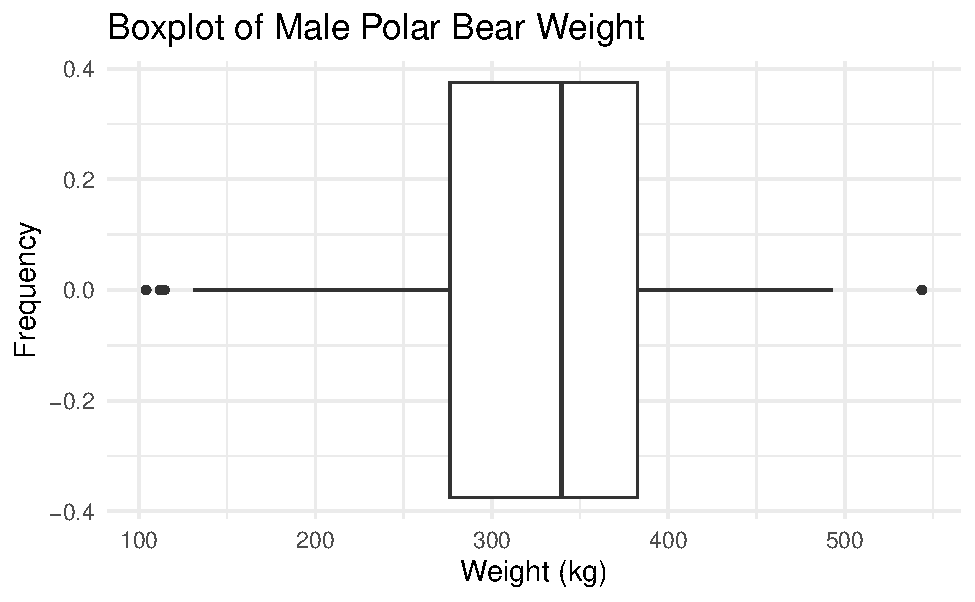
\includegraphics[width=0.6\linewidth]{11-LN011-paired_files/figure-latex/unnamed-chunk-2-2} \end{center}

Summary Statistics:

\begin{Shaded}
\begin{Highlighting}[]
\NormalTok{pb }\SpecialCharTok{\%\textgreater{}\%}
  \FunctionTok{summarise}\NormalTok{(}\FunctionTok{favstats}\NormalTok{(Weight)) }\CommentTok{\#Gives the summary statistics}
\CommentTok{\#\textgreater{}     min    Q1 median     Q3   max     mean       sd  n missing}
\CommentTok{\#\textgreater{} 1 104.1 276.3  339.4 382.45 543.6 324.5988 88.32615 83       0}
\end{Highlighting}
\end{Shaded}

\hypertarget{confidence-interval-1}{%
\subsection*{Confidence interval}\label{confidence-interval-1}}
\addcontentsline{toc}{subsection}{Confidence interval}

\hypertarget{simulation-based-method-2}{%
\subsubsection*{Simulation-based method}\label{simulation-based-method-2}}
\addcontentsline{toc}{subsubsection}{Simulation-based method}

\begin{itemize}
\item
  Label cards with the values from the data set
\item
  Sample with replacement (bootstrap) from the original sample \(n\) times
\item
  Plot the simulated sample mean on the bootstrap distribution
\item
  Repeat at least 1000 times (simulations)
\item
  Find the cut-offs for the middle X\% (confidence level) in a bootstrap distribution.
\item
  ie. 95\% CI = (2.5th percentile, 97.5th percentile)
\end{itemize}

Conditions for inference for a single mean:

\begin{itemize}
\tightlist
\item
  Independence:
\end{itemize}

\vspace{0.5in}

\begin{Shaded}
\begin{Highlighting}[]
\FunctionTok{set.seed}\NormalTok{(}\DecValTok{216}\NormalTok{)}
\FunctionTok{paired\_bootstrap\_CI}\NormalTok{(}\AttributeTok{data =}\NormalTok{ pb}\SpecialCharTok{$}\NormalTok{Weight, }\CommentTok{\# Enter vector of differences}
            \AttributeTok{number\_repetitions =} \DecValTok{1000}\NormalTok{, }\CommentTok{\# Number of bootstrap samples for CI}
            \AttributeTok{confidence\_level =} \FloatTok{0.95}\NormalTok{,  }\CommentTok{\# Confidence level in decimal form}
            \AttributeTok{which\_first =} \DecValTok{1}\NormalTok{)  }\CommentTok{\# Not needed when entering vector of differences}
\end{Highlighting}
\end{Shaded}

\begin{center}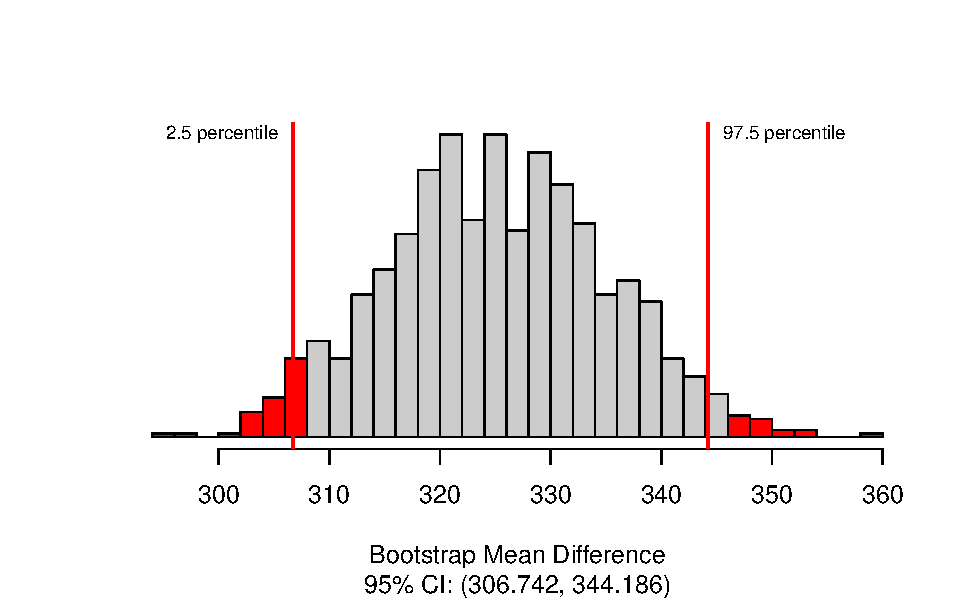
\includegraphics[width=0.7\linewidth]{11-LN011-paired_files/figure-latex/unnamed-chunk-4-1} \end{center}

The confidence interval estimates the \_\_\_\_\_\_\_\_\_\_\_\_\_\_\_\_
of \_\_\_\_\_\_\_\_\_\_\_\_\_\_\_\_\_\_\_\_.

Confidence interval interpretation:

\begin{itemize}
\item
  How confident you are (e.g., 90\%, 95\%, 98\%, 99\%)
\item
  Parameter of interest
\item
  Calculated interval
\item
  Order of subtraction when comparing two groups
\end{itemize}

\vspace{0.8in}

\newpage

\hypertarget{theory-based-method-1}{%
\subsubsection*{Theory-based method}\label{theory-based-method-1}}
\addcontentsline{toc}{subsubsection}{Theory-based method}

\begin{itemize}
\tightlist
\item
  Calculate the interval centered at the sample statistic
\end{itemize}

\rgi \(\text{statistic} \pm \text{margin of error}\)

\vspace{0.8in}

Conditions for inference using theory-based methods:

\begin{itemize}
\tightlist
\item
  Independence:
\end{itemize}

\vspace{0.2in}

\begin{itemize}
\tightlist
\item
  Large enough sample size:
\end{itemize}

\vspace{0.2in}

\hypertarget{t---distribution}{%
\subsection*{T - distribution}\label{t---distribution}}
\addcontentsline{toc}{subsection}{T - distribution}

In the theoretical approach, we use the CLT to tell us that the distribution of sample means will be approximately normal, centered at the assumed true mean under \(H_0\) and with standard deviation \(\frac{\sigma}{\sqrt{n}}\).

\[\bar{x} \sim N(\mu_0, \frac{\sigma}{\sqrt{n}})\]
\setstretch{1.5}

\begin{itemize}
\item
  Estimate the population standard deviation, \(\sigma\), with the
  \_\_\_\_\_\_\_\_\_\_\_\_\_\_\_\_\_\_\_\_\_\_\_\_\_\_\_ standard deviation, \_\_\_\_\_\_\_\_.
\item
  For a single quantitative variable we use the \_\_\_\_ - distribution
  with \_\_\_\_\_\_\_\_\_\_\_\_\_\_\_
  degrees of freedom to approximate the sampling distribution.
\end{itemize}

\setstretch{1}

The \(t^*\) multiplier is the value at the given percentile of the t-distribution with \(n - 1\) degrees of freedom.

\begin{center}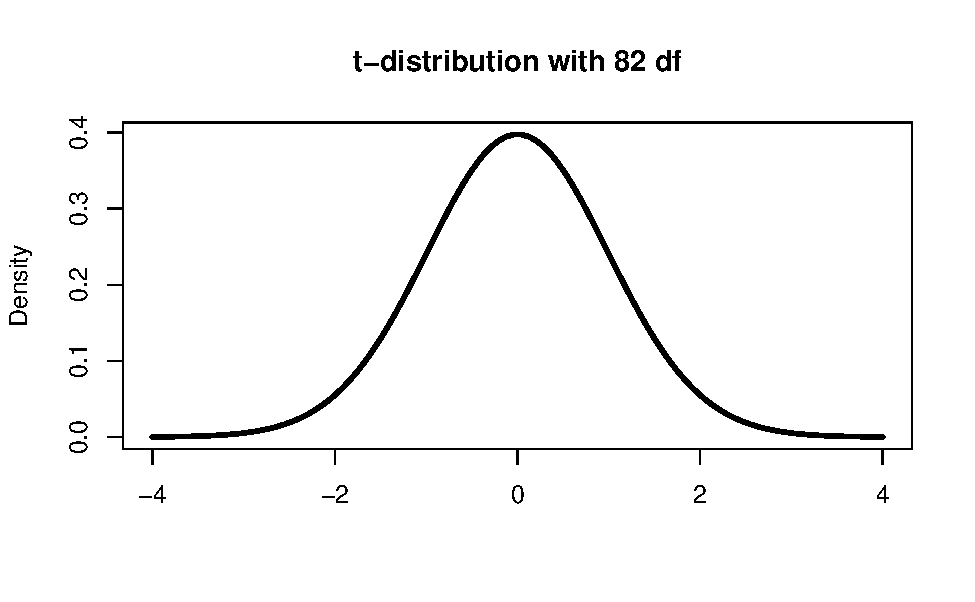
\includegraphics[width=0.7\linewidth]{11-LN011-paired_files/figure-latex/tstarpb-1} \end{center}

\newpage

To find the \(t^*\) multiplier for a 95\% confidence interval:

\begin{Shaded}
\begin{Highlighting}[]
\FunctionTok{qt}\NormalTok{(}\FloatTok{0.975}\NormalTok{, }\AttributeTok{df =} \DecValTok{82}\NormalTok{)}
\CommentTok{\#\textgreater{} [1] 1.989319}
\end{Highlighting}
\end{Shaded}

Calculation of the confidence interval for the true mean weight of polar bears from the Southern Beaufort Sea:

\vspace{0.8in}

\hypertarget{hypothesis-testing-2}{%
\subsection*{Hypothesis testing}\label{hypothesis-testing-2}}
\addcontentsline{toc}{subsection}{Hypothesis testing}

\setstretch{1.5}

\begin{itemize}
\tightlist
\item
  Hypotheses are always written about the \_\_\_\_\_\_\_\_\_\_\_\_\_\_\_\_\_\_\_\_\_\_\_\_\_. For a single mean we will use the notation \_\_\_\_\_\_\_\_\_\_\_.
\end{itemize}

\setstretch{1}

Null Hypothesis:

\(H_0:\)

\vspace{0.2in}

Alternative Hypothesis:

\(H_A:\)

\vspace{0.2in}

\setstretch{1.5}

\begin{itemize}
\tightlist
\item
  Direction of the alternative depends on the \_\_\_\_\_\_\_\_\_\_\_\_\_\_\_\_\_\_
  \_\_\_\_\_\_\_\_\_\_\_\_\_\_\_\_\_\_\_.
\end{itemize}

\setstretch{1}

\hypertarget{simulation-based-method-3}{%
\subsubsection*{Simulation-based method}\label{simulation-based-method-3}}
\addcontentsline{toc}{subsubsection}{Simulation-based method}

\begin{itemize}
\item
  Simulate many samples assuming \(H_0: \mu = \mu_0\)

  \begin{itemize}
  \item
    Shift the data by the difference between \(\mu_0\) and \(\bar{x}\)
  \item
    Sample with replacement \(n\) times from the shifted data
  \item
    Plot the simulated shifted sample mean from each simulation
  \item
    Repeat 1000 times (simulations) to create the null distribution
  \item
    Find the proportion of simulations at least as extreme as \(\bar{x}\)
  \end{itemize}
\end{itemize}

Example: Is there evidence that male polar bears weigh less than 370kg (previously recorded measure), on average? The weight was measured on a representative sample of 83 male polar bears from the Southern Beaufort Sea.

Hypotheses:

In notation:

\(H_0:\)

\vspace{0.2in}

\(H_A:\)

\vspace{0.2in}

\newpage

In words:

\(H_0:\)

\vspace{0.6in}

\(H_A:\)

\vspace{0.6in}

Reminder of summary statistics:

\begin{Shaded}
\begin{Highlighting}[]
\NormalTok{pb }\SpecialCharTok{\%\textgreater{}\%}
  \FunctionTok{summarise}\NormalTok{(}\FunctionTok{favstats}\NormalTok{(Weight)) }\CommentTok{\#Gives the summary statistics}
\CommentTok{\#\textgreater{}     min    Q1 median     Q3   max     mean       sd  n missing}
\CommentTok{\#\textgreater{} 1 104.1 276.3  339.4 382.45 543.6 324.5988 88.32615 83       0}
\end{Highlighting}
\end{Shaded}

Find the difference:

\(\mu_0 - \bar{x} =\)

\begin{Shaded}
\begin{Highlighting}[]
\FunctionTok{set.seed}\NormalTok{(}\DecValTok{216}\NormalTok{)}
\FunctionTok{paired\_test}\NormalTok{(}\AttributeTok{data =}\NormalTok{ pb}\SpecialCharTok{$}\NormalTok{Weight,   }\CommentTok{\# Vector of differences }
                                         \CommentTok{\# or data set with column for each group}
            \AttributeTok{shift =} \FloatTok{45.4}\NormalTok{,   }\CommentTok{\# Shift needed for bootstrap hypothesis test}
            \AttributeTok{as\_extreme\_as =} \FloatTok{324.6}\NormalTok{,  }\CommentTok{\# Observed statistic}
            \AttributeTok{direction =} \StringTok{"less"}\NormalTok{,  }\CommentTok{\# Direction of alternative}
            \AttributeTok{number\_repetitions =} \DecValTok{1000}\NormalTok{,  }\CommentTok{\# Number of simulated samples for null distribution}
            \AttributeTok{which\_first =} \DecValTok{1}\NormalTok{)  }\CommentTok{\# Not needed when using calculated differences}
\end{Highlighting}
\end{Shaded}

\begin{center}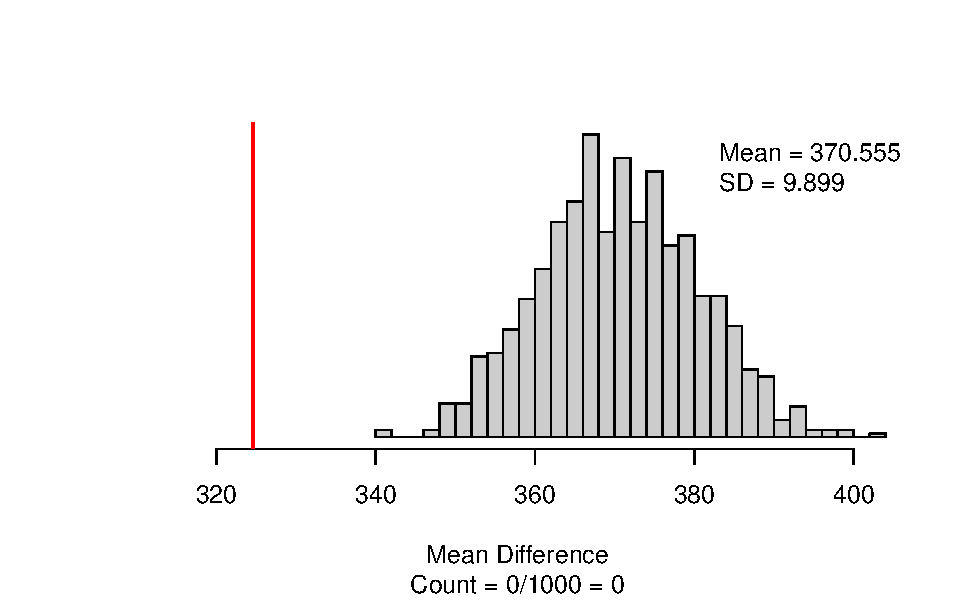
\includegraphics[width=0.6\linewidth]{11-LN011-paired_files/figure-latex/unnamed-chunk-7-1} \end{center}

\newpage

Interpretation of the p-value:

\begin{itemize}
\item
  Statement about probability or proportion of samples
\item
  Statistic (summary measure and value)
\item
  Direction of the alternative
\item
  Null hypothesis (in context)
\end{itemize}

\vspace{0.8in}

Conclusion:

\begin{itemize}
\item
  Amount of evidence
\item
  Parameter of interest
\item
  Direction of the alternative hypothesis
\end{itemize}

\vspace{0.8in}

\hypertarget{theory-based-method-2}{%
\subsubsection*{Theory-based method}\label{theory-based-method-2}}
\addcontentsline{toc}{subsubsection}{Theory-based method}

\begin{itemize}
\item
  Calculate the standardized statistic
\item
  Find the area under the t-distribution with \(n - 1\) df at least as extreme as the standardized statistic
\end{itemize}

Equation for the standard error of the sample mean:

\vspace{0.5in}

Equation for the standardized sample mean:

\vspace{0.5in}

Calculate the standardized sample mean weight of adult male polar bears:

\vspace{0.4in}

\begin{center}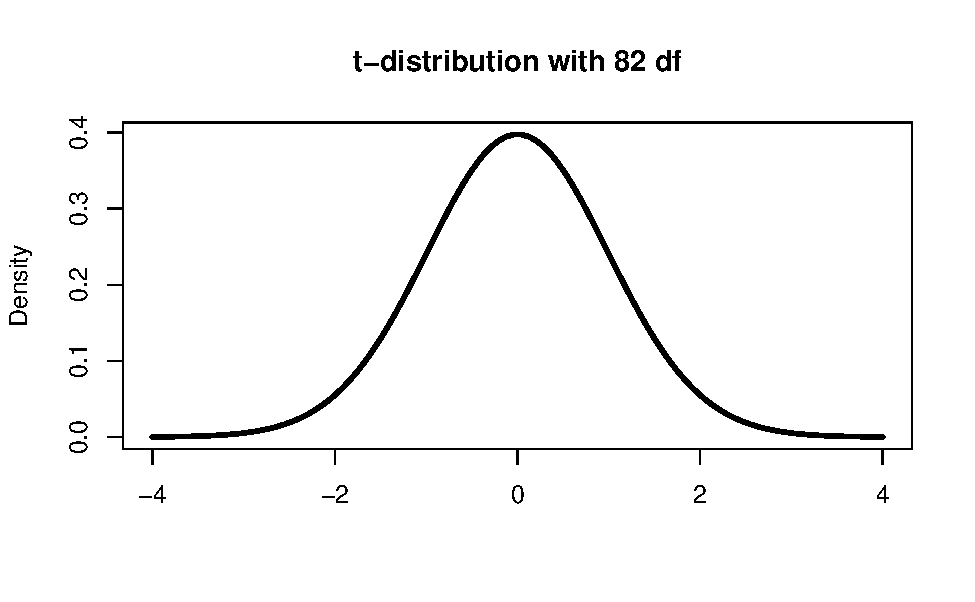
\includegraphics[width=0.7\linewidth]{11-LN011-paired_files/figure-latex/pvaluepb-1} \end{center}

Interpret the standardized sample mean weight:

\vspace{0.8in}

To find the theory-based p-value:

\begin{Shaded}
\begin{Highlighting}[]
\FunctionTok{pt}\NormalTok{(}\SpecialCharTok{{-}}\FloatTok{4.683}\NormalTok{, }\AttributeTok{df=}\DecValTok{82}\NormalTok{, }\AttributeTok{lower.tail=}\ConstantTok{TRUE}\NormalTok{)}
\CommentTok{\#\textgreater{} [1] 5.531605e{-}06}
\end{Highlighting}
\end{Shaded}

\hypertarget{paired-vs.-independent-samples}{%
\subsection{Paired vs.~Independent Samples}\label{paired-vs.-independent-samples}}

Two groups are paired if an observational unit in one group is connected to an observational unit in another group

\rgi Data is paired if the samples are \_\_\_\_\_\_\_\_\_\_\_\_\_\_\_\_\_\_\_

Examples:

\begin{itemize}
\item
  Change in test score from pre and post test
\item
  Weight of college students before and after 1st year
\item
  Change in blood pressure
\end{itemize}

Example: Three hundred registered voters were selected at random to participate in a study on attitudes about how well the president is performing. They were each asked to answer a short multiple-choice questionnaire and then they watched a 20-minute video that presented information about the job description of the president. After watching the video, the same 300 selected voters were asked to answer a follow-up multiple-choice questionnaire.

\begin{itemize}
\tightlist
\item
  Is this an example of a paired samples or independent samples study?
\end{itemize}

\vspace{0.2in}

Thirty dogs were selected at random from those residing at the humane society last month. The 30 dogs were split at random into two groups. The first group of 15 dogs was trained to perform a certain task using a reward method. The second group of 15 dogs was trained to perform the same task using a reward-punishment method.

\begin{itemize}
\tightlist
\item
  Is this an example of a paired samples or independent samples study?
\end{itemize}

\vspace{0.2in}

Fifty skiers volunteered to study how different waxes impacted their downhill race times. The participants were split into groups of two based on similar race times from the previous race. One of the two then had their skis treated with Wax A while the other was treated with Wax B. The downhill ski race times were then measured for each of the 25 volunteers who used Wax A as well as for each of the 25 volunteers who used Wax B.

\begin{itemize}
\tightlist
\item
  Is this an example of a paired samples or independent samples study?
\end{itemize}

\vspace{0.2in}

For a paired experiment, we look at the difference between responses for each unit (pair), rather than just the average difference between treatment groups

\setstretch{1.5}

\begin{itemize}
\item
  The summary measure for paired data is the \_\_\_\_\_\_\_\_\_\_\_\_\_\_\_\_\_\_\_\_\_\_\_.
\item
  Mean difference: the average \_\_\_\_\_\_\_\_\_\_\_\_\_\_\_ in the \_\_\_\_\_\_\_\_\_\_\_\_\_\_\_\_\_
  variable outcomes for observational units between \_\_\_\_\_\_\_\_\_\_\_\_\_\_\_\_\_\_\_\_ variable groups
\end{itemize}

\setstretch{1}

Parameter of Interest:

\begin{itemize}
\item
  Include:

  \begin{itemize}
  \item
    Reference of the population (true, long-run, population, all)
  \item
    Summary measure
  \item
    Context

    \begin{itemize}
    \item
      Observational units/cases
    \item
      Response variable (and explanatory variable if present)

      \begin{itemize}
      \tightlist
      \item
        If the response variable is categorical, define a `success' in context
      \end{itemize}
    \end{itemize}
  \end{itemize}
\end{itemize}

\(\mu_d:\)

\vspace{0.5in}

Notation for the Sample Statistics

\begin{itemize}
\item
  Sample mean of the differences:
\item
  Sample standard deviation of the differences:
\end{itemize}

\newpage

Example: Is there a difference in heights between husbands and wives? The heights were measured on the husband and wife in a random sample of 199 married couples from Great Britain.

Parameter of interest:

\vspace{0.8in}

\begin{Shaded}
\begin{Highlighting}[]
\NormalTok{hw }\OtherTok{\textless{}{-}}\FunctionTok{read.csv}\NormalTok{(}\StringTok{"data/husbands\_wives\_ht.csv"}\NormalTok{)}
\FunctionTok{paired\_observed\_plot}\NormalTok{(hw)}
\end{Highlighting}
\end{Shaded}

\begin{center}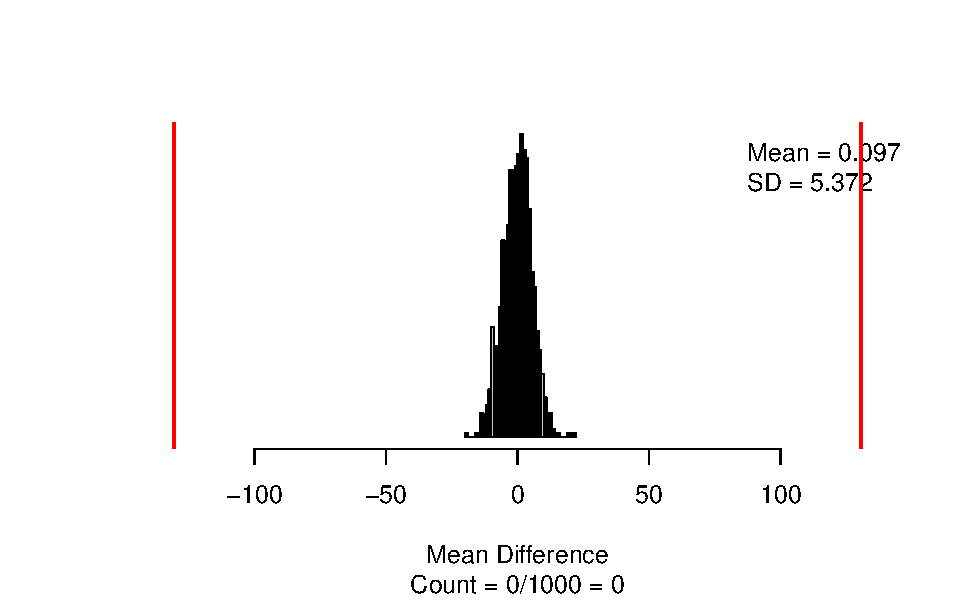
\includegraphics[width=0.7\linewidth]{11-LN011-paired_files/figure-latex/unnamed-chunk-9-1} \end{center}

\begin{Shaded}
\begin{Highlighting}[]
\NormalTok{hw\_diff }\OtherTok{\textless{}{-}}\NormalTok{ hw }\SpecialCharTok{\%\textgreater{}\%}
  \FunctionTok{select}\NormalTok{(ht\_husband, ht\_wife) }\SpecialCharTok{\%\textgreater{}\%}
  \FunctionTok{mutate}\NormalTok{(}\AttributeTok{ht\_diff =}\NormalTok{ ht\_husband}\SpecialCharTok{{-}}\NormalTok{ht\_wife)}
\end{Highlighting}
\end{Shaded}

\begin{Shaded}
\begin{Highlighting}[]
\NormalTok{hw\_diff }\SpecialCharTok{\%\textgreater{}\%}
    \FunctionTok{summarise}\NormalTok{(}\FunctionTok{favstats}\NormalTok{(ht\_husband))}
\CommentTok{\#\textgreater{}    min   Q1 median   Q3  max     mean       sd   n missing}
\CommentTok{\#\textgreater{} 1 1559 1691   1725 1774 1949 1732.492 68.75067 199       0}
\end{Highlighting}
\end{Shaded}

\begin{Shaded}
\begin{Highlighting}[]
\NormalTok{hw\_diff }\SpecialCharTok{\%\textgreater{}\%}
    \FunctionTok{summarise}\NormalTok{(}\FunctionTok{fav\_stats}\NormalTok{(ht\_wife))}
\CommentTok{\#\textgreater{}    min   Q1 median   Q3  max    mean     sd   n missing}
\CommentTok{\#\textgreater{} 1 1410 1560   1600 1650 1760 1601.95 62.435 199       0}
\end{Highlighting}
\end{Shaded}

\begin{Shaded}
\begin{Highlighting}[]
\NormalTok{hw\_diff }\SpecialCharTok{\%\textgreater{}\%}
    \FunctionTok{summarise}\NormalTok{(}\FunctionTok{fav\_stats}\NormalTok{(ht\_diff))}
\CommentTok{\#\textgreater{}   min   Q1 median  Q3 max     mean       sd   n missing}
\CommentTok{\#\textgreater{} 1 {-}96 83.5    131 179 303 130.5427 74.13608 199       0}
\end{Highlighting}
\end{Shaded}

\newpage

\hypertarget{hypothesis-testing-3}{%
\subsection*{Hypothesis testing}\label{hypothesis-testing-3}}
\addcontentsline{toc}{subsection}{Hypothesis testing}

Null hypothesis assumes ``no effect'', ``no difference'', ``nothing interesting happening'', etc.

\begin{itemize}
\item
  Treat the differences like a single mean
\item
  Always of form: ``parameter'' = null value
\end{itemize}

\(H_0:\)

\vspace{0.2in}

\(H_A:\)

\vspace{0.2in}

\begin{itemize}
\tightlist
\item
  Research question determines the alternative hypothesis.
\end{itemize}

Write the null and alternative for the height study:

In words:

\(H_0:\)

\vspace{0.5in}

\(H_A:\)

\vspace{0.5in}

In notation:

\(H_0:\)

\vspace{0.2in}

\(H_A:\)

\vspace{0.2in}

\hypertarget{simulation-based-method-4}{%
\subsubsection*{Simulation-based method}\label{simulation-based-method-4}}
\addcontentsline{toc}{subsubsection}{Simulation-based method}

Simulated null distribution:

\begin{Shaded}
\begin{Highlighting}[]
\FunctionTok{set.seed}\NormalTok{(}\DecValTok{216}\NormalTok{)}
\FunctionTok{paired\_test}\NormalTok{(}\AttributeTok{data =}\NormalTok{ hw\_diff}\SpecialCharTok{$}\NormalTok{ht\_diff,   }\CommentTok{\# Vector of differences }
                                         \CommentTok{\# or data set with column for each group}
            \AttributeTok{shift =} \SpecialCharTok{{-}}\FloatTok{130.543}\NormalTok{,   }\CommentTok{\# Shift needed for bootstrap hypothesis test}
            \AttributeTok{as\_extreme\_as =} \FloatTok{130.543}\NormalTok{,  }\CommentTok{\# Observed statistic}
            \AttributeTok{direction =} \StringTok{"two{-}sided"}\NormalTok{,  }\CommentTok{\# Direction of alternative}
            \AttributeTok{number\_repetitions =} \DecValTok{1000}\NormalTok{,  }\CommentTok{\# Number of simulated samples for null distribution}
            \AttributeTok{which\_first =} \DecValTok{1}\NormalTok{)  }\CommentTok{\# Not needed when using calculated differences}
\end{Highlighting}
\end{Shaded}

\begin{center}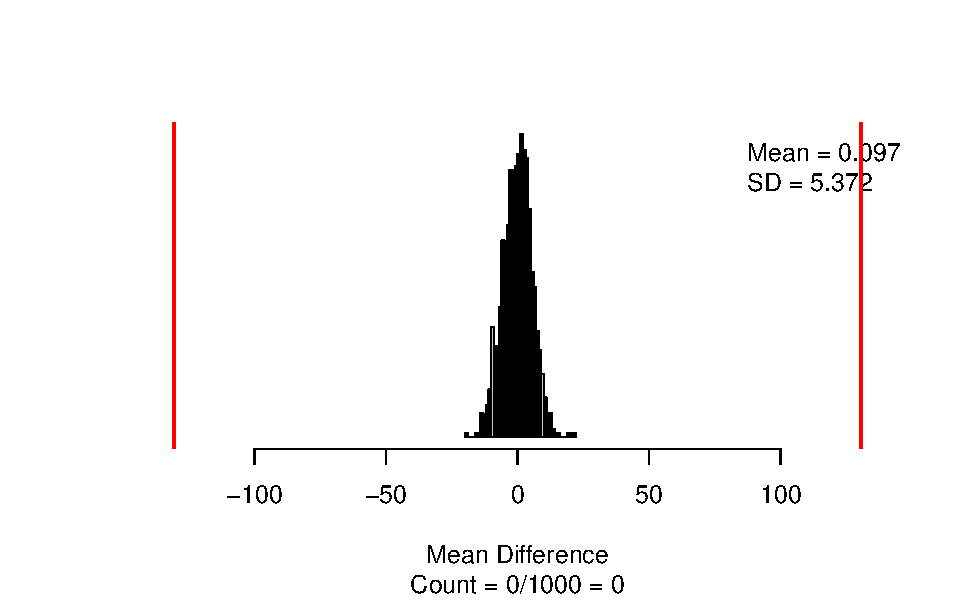
\includegraphics[width=0.7\linewidth]{11-LN011-paired_files/figure-latex/unnamed-chunk-14-1} \end{center}

Interpret the p-value:

\begin{itemize}
\item
  Statement about probability or proportion of samples
\item
  Statistic (summary measure and value)
\item
  Direction of the alternative
\item
  Null hypothesis (in context)
\end{itemize}

\vspace{0.8in}

Conclusion:

\begin{itemize}
\item
  Amount of evidence
\item
  Parameter of interest
\item
  Direction of the alternative hypothesis
\end{itemize}

\vspace{0.8in}

\hypertarget{confidence-interval-2}{%
\subsection*{Confidence interval}\label{confidence-interval-2}}
\addcontentsline{toc}{subsection}{Confidence interval}

Simulated bootstrap distribution:

\begin{Shaded}
\begin{Highlighting}[]
\FunctionTok{set.seed}\NormalTok{(}\DecValTok{216}\NormalTok{)}
\FunctionTok{paired\_bootstrap\_CI}\NormalTok{(}\AttributeTok{data =}\NormalTok{ hw\_diff}\SpecialCharTok{$}\NormalTok{ht\_diff, }\CommentTok{\# Enter vector of differences}
            \AttributeTok{number\_repetitions =} \DecValTok{1000}\NormalTok{, }\CommentTok{\# Number of bootstrap samples for CI}
            \AttributeTok{confidence\_level =} \FloatTok{0.99}\NormalTok{,  }\CommentTok{\# Confidence level in decimal form}
            \AttributeTok{which\_first =} \DecValTok{1}\NormalTok{)  }\CommentTok{\# Not needed when entering vector of differences}
\end{Highlighting}
\end{Shaded}

\begin{center}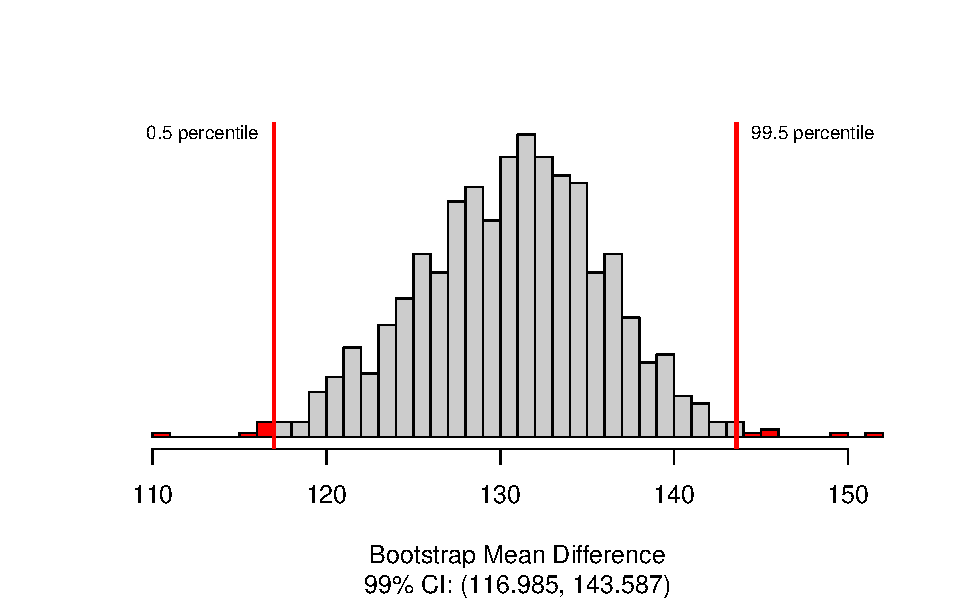
\includegraphics[width=0.7\linewidth]{11-LN011-paired_files/figure-latex/unnamed-chunk-15-1} \end{center}

Interpret the 99\% confidence interval:

\begin{itemize}
\item
  How confident you are (e.g., 90\%, 95\%, 98\%, 99\%)
\item
  Parameter of interest
\item
  Calculated interval
\item
  Order of subtraction when comparing two groups
\end{itemize}

\vspace{0.8in}

\hypertarget{theory-based-method-3}{%
\subsubsection*{Theory-based method}\label{theory-based-method-3}}
\addcontentsline{toc}{subsubsection}{Theory-based method}

\begin{Shaded}
\begin{Highlighting}[]
\NormalTok{hw\_diff }\SpecialCharTok{\%\textgreater{}\%}
    \FunctionTok{summarise}\NormalTok{(}\FunctionTok{fav\_stats}\NormalTok{(ht\_diff))}
\CommentTok{\#\textgreater{}   min   Q1 median  Q3 max     mean       sd   n missing}
\CommentTok{\#\textgreater{} 1 {-}96 83.5    131 179 303 130.5427 74.13608 199       0}
\end{Highlighting}
\end{Shaded}

Check the conditions to use theory-based methods:

\vspace{1in}

Calculate the standardized sample mean difference in height:

\vspace{1in}

Interpret the standardized statistic:

\vspace{0.8in}

What theoretical distribution should we use to find the p-value using the value of the standardized statistic?

\vspace{0.3in}

To find the p-value:

\begin{Shaded}
\begin{Highlighting}[]
\FunctionTok{pt}\NormalTok{(}\FloatTok{24.84}\NormalTok{, }\AttributeTok{df =} \DecValTok{198}\NormalTok{, }\AttributeTok{lower.tail=}\ConstantTok{FALSE}\NormalTok{)}\SpecialCharTok{*}\DecValTok{2}
\CommentTok{\#\textgreater{} [1] 9.477617e{-}63}
\end{Highlighting}
\end{Shaded}

Calculate a 99\% confidence interval:

\begin{itemize}
\tightlist
\item
  First need to find the \(t*\) multiplier from the t-distribution with 198 df
\end{itemize}

\begin{Shaded}
\begin{Highlighting}[]
\FunctionTok{qt}\NormalTok{(}\FloatTok{0.995}\NormalTok{, }\AttributeTok{df=}\DecValTok{198}\NormalTok{, }\AttributeTok{lower.tail =} \ConstantTok{TRUE}\NormalTok{)}
\CommentTok{\#\textgreater{} [1] 2.600887}
\end{Highlighting}
\end{Shaded}

Calculate the margin of error:
\vspace{0.4in}

Calculate the theory-based confidence interval.
\vspace{0.5in}
\newpage

\hypertarget{out-of-class-activity-11-color-interference}{%
\section{Out of Class Activity 11: Color Interference}\label{out-of-class-activity-11-color-interference}}

\setstretch{1}

\hypertarget{learning-outcomes-3}{%
\subsection{Learning outcomes}\label{learning-outcomes-3}}

\begin{itemize}
\item
  Given a research question involving paired differences, construct the null and alternative hypotheses
  in words and using appropriate statistical symbols.
\item
  Describe and perform a theory-based hypothesis test for a paired mean difference.
\item
  Interpret and evaluate a p-value for a theory-based hypothesis test for a paired mean difference.
\item
  Use theory-based methods to find a confidence interval for a paired mean difference.
\item
  Interpret a confidence interval for a paired mean difference.
\item
  Use a confidence interval to determine the conclusion of a hypothesis test.
\end{itemize}

\hypertarget{terminology-review-2}{%
\subsection{Terminology review}\label{terminology-review-2}}

In today's activity, we will analyze paired quantitative data using theory-based methods. Some terms covered in this activity are:

\begin{itemize}
\item
  Paired data
\item
  Mean difference
\item
  Independent observational units
\item
  Normality
\item
  \(t\)-distribution
\item
  Degrees of freedom
\item
  T-score
\end{itemize}

To review these concepts, see Chapter 18 in the textbook.

\hypertarget{color-interference}{%
\subsection{Color Interference}\label{color-interference}}

The abstract of the article ``Studies of interference in serial verbal reactions'' in the \emph{Journal of Experimental Psychology} (Stroop 1935) reads:

\begin{quote}
In this study pairs of conflicting stimuli, both being inherent aspects of the same symbols, were presented simultaneously (a name of one color printed in the ink of another color---a word stimulus and a color stimulus).
The difference in time for reading the words printed in colors and the same words printed in black is the measure of interference of color stimuli upon reading words. \ldots{}
The interference of conflicting color stimuli upon the time for reading 100 words (each word naming a color unlike the ink-color of its print) caused an increase of 2.3 seconds or 5.6\% over the normal time for reading the same words printed in black.
\end{quote}

The article reports on the results of a study in which seventy college undergraduates were given forms with 100 names of colors written in black ink, and the same 100 names of colors written in another color (i.e., the word purple written in green ink). The total time (in seconds) for reading the 100 words printed in black, and the total time (in seconds) for reading the 100 words printed in different colors were recorded for each subject. The order in which the forms (black or color) were given was randomized to the subjects. Does printing the name of colors in a different color increase the time it takes to read the words? Use color - black as the order of subtraction.

\hypertarget{identify-the-scenario}{%
\subsubsection*{Identify the scenario}\label{identify-the-scenario}}
\addcontentsline{toc}{subsubsection}{Identify the scenario}

\begin{enumerate}
\def\labelenumi{\arabic{enumi}.}
\tightlist
\item
  Should these observations be considered paired or independent? Explain your answer.
  \vspace{0.5in}
\end{enumerate}

\hypertarget{ask-a-research-question-1}{%
\subsubsection*{Ask a research question}\label{ask-a-research-question-1}}
\addcontentsline{toc}{subsubsection}{Ask a research question}

\begin{enumerate}
\def\labelenumi{\arabic{enumi}.}
\setcounter{enumi}{1}
\tightlist
\item
  Write out the null hypothesis in words, in the context of this study.
\end{enumerate}

\vspace{0.8in}

\begin{enumerate}
\def\labelenumi{\arabic{enumi}.}
\setcounter{enumi}{2}
\tightlist
\item
  Write out the alternative hypothesis in proper notation for this study.
\end{enumerate}

\vspace{0.5in}

In general, the sampling distribution for a sample mean, \(\bar{x}\), based on a sample of size \(n\) from a population with a true mean \(\mu\) and true standard deviation \(\sigma\) can be modeled using a Normal distribution when certain conditions are met.

Conditions for the sampling distribution of \(\bar{x}\) to follow an approximate Normal distribution:

\begin{itemize}
\item
  \textbf{Independence}: The sample's observations are independent. For paired data, that means each pairwise difference should be independent.
\item
  \textbf{Normality}: The data should be approximately normal or the sample size should be large.

  \begin{itemize}
  \item
    \(n < 30\): If the sample size \(n\) is less than 30 and the distribution of the data is approximately normal with no clear outliers in the data, then we typically assume the data come from a nearly normal distribution to satisfy the condition.
  \item
    \(n \geq 30\): If the sample size \(n\) is at least 30 and there are no particularly extreme outliers in the data, then we typically assume the sampling distribution of \(\bar{x}\) is nearly normal, even if the underlying distribution of individual observations is not.
  \item
    \(n \geq 100\): If the sample size \(n\) is at least 100 (regardless of the presence of skew or outliers), we typically assume the sampling distribution of \(\bar{x}\) is nearly normal, even if the underlying distribution of individual observations is not.
  \end{itemize}
\end{itemize}

\begin{figure}

{\centering 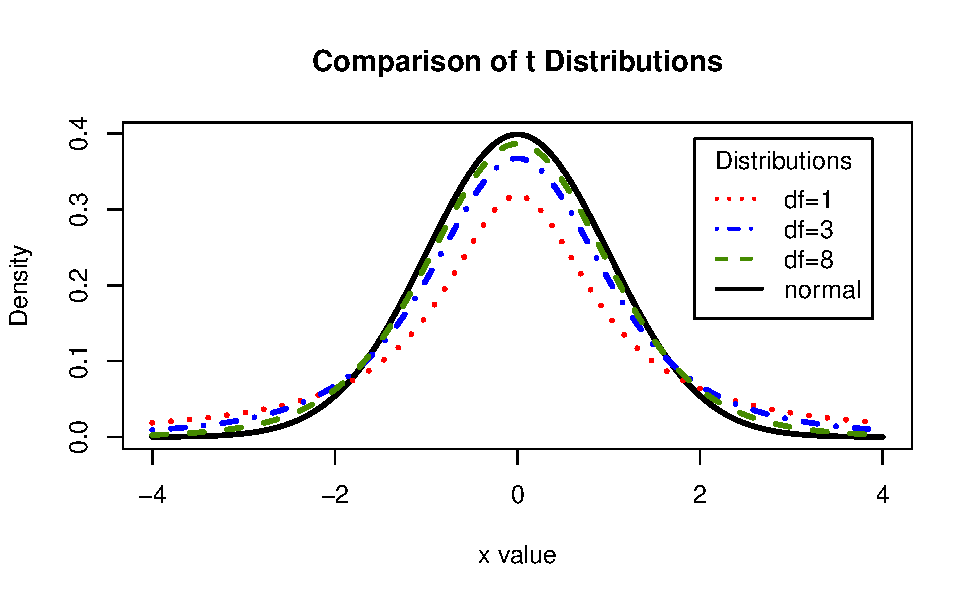
\includegraphics[width=0.7\linewidth]{11-OCA08-paired-theory_files/figure-latex/tdist-1} 

}

\caption{Comparison of the standard Normal vs t-distribution with various degrees of freedom}\label{fig:tdist}
\end{figure}

Like we saw in Chapter \textbf{5}, we will not know the values of the parameters and must use the sample data to estimate them. Unlike with proportions, in which we only needed to estimate the population proportion, \(\pi\), quantitative sample data must be used to estimate both a population mean \(\mu\) and a population standard deviation \(\sigma\). This additional uncertainty will require us to use a theoretical distribution that is just a bit wider than the Normal distribution. Enter the \textbf{\(t\)-distribution}!

As you can seen from Figure \ref{fig:tdist}, the \(t\)-distributions (dashed and dotted lines) are centered at 0 just like a standard Normal distribution (solid line), but are slightly wider. The variability of a \(t\)-distribution depends on its degrees of freedom, which is calculated from the sample size of a study. (For a single sample of \(n\) observations or paired differences, the degrees of freedom is equal to \(n-1\).) Recall from previous classes that larger sample sizes tend to result in narrower sampling distributions. We see that here as well. The larger the sample size, the larger the degrees of freedom, the narrower the \(t\)-distribution. (In fact, a \(t\)-distribution with infinite degrees of freedom actually IS the standard Normal distribution!)

\hypertarget{summarize-and-visualize-the-data-1}{%
\subsubsection*{Summarize and visualize the data}\label{summarize-and-visualize-the-data-1}}
\addcontentsline{toc}{subsubsection}{Summarize and visualize the data}

Since the original data from the study are not available, we simulated data to match the means and standard deviations reported in the article. We will use these simulated data in the analysis below.

The following code plots each subject's time to read the colored words (above) and time to read the black words (below) connected by a grey line, a histogram of the differences in time to read words between the two conditions, and a boxplot displaying the pairwise differences in time (color \(-\) black).

\begin{Shaded}
\begin{Highlighting}[]
\NormalTok{color }\OtherTok{\textless{}{-}} \FunctionTok{read.csv}\NormalTok{(}\StringTok{"https://math.montana.edu/courses/s216/data/interference.csv"}\NormalTok{)}
\FunctionTok{paired\_observed\_plot}\NormalTok{(color)}

\NormalTok{color\_diff }\OtherTok{\textless{}{-}}\NormalTok{ color }\SpecialCharTok{\%\textgreater{}\%} 
  \FunctionTok{mutate}\NormalTok{(}\AttributeTok{differences =}\NormalTok{ DiffCol}\SpecialCharTok{{-}}\NormalTok{Black)}
\NormalTok{color\_diff }\SpecialCharTok{\%\textgreater{}\%}
  \FunctionTok{ggplot}\NormalTok{(}\FunctionTok{aes}\NormalTok{(}\AttributeTok{x =}\NormalTok{ differences))}\SpecialCharTok{+}
  \FunctionTok{geom\_boxplot}\NormalTok{()}\SpecialCharTok{+}
  \FunctionTok{labs}\NormalTok{(}\AttributeTok{title=}\StringTok{"Boxplot of the pairwise differences"}\NormalTok{,}
       \AttributeTok{x =} \StringTok{"Differences in time to read words (Color {-} Black)"}\NormalTok{)}
\end{Highlighting}
\end{Shaded}

\begin{center}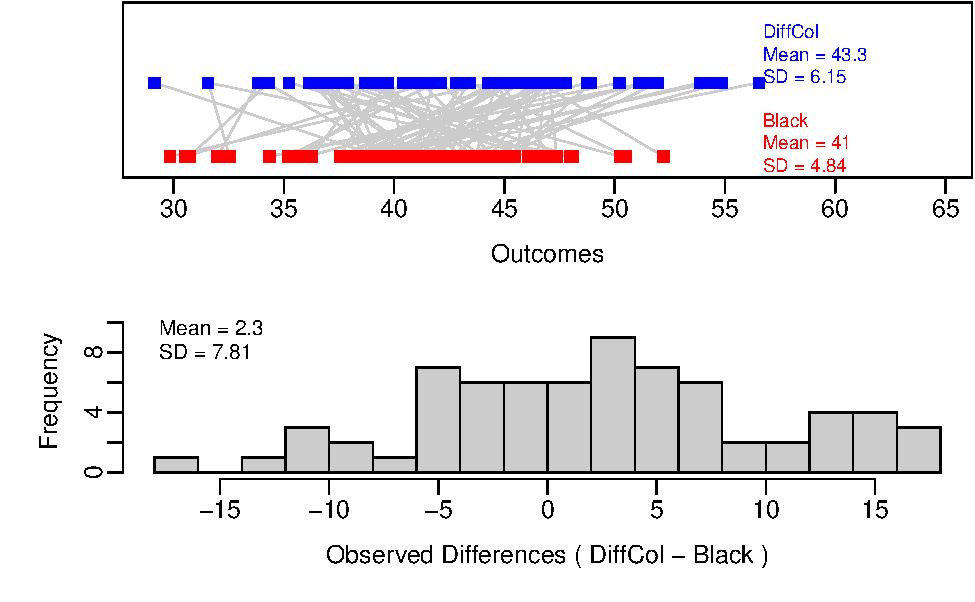
\includegraphics[width=0.7\linewidth]{11-OCA08-paired-theory_files/figure-latex/unnamed-chunk-1-1} 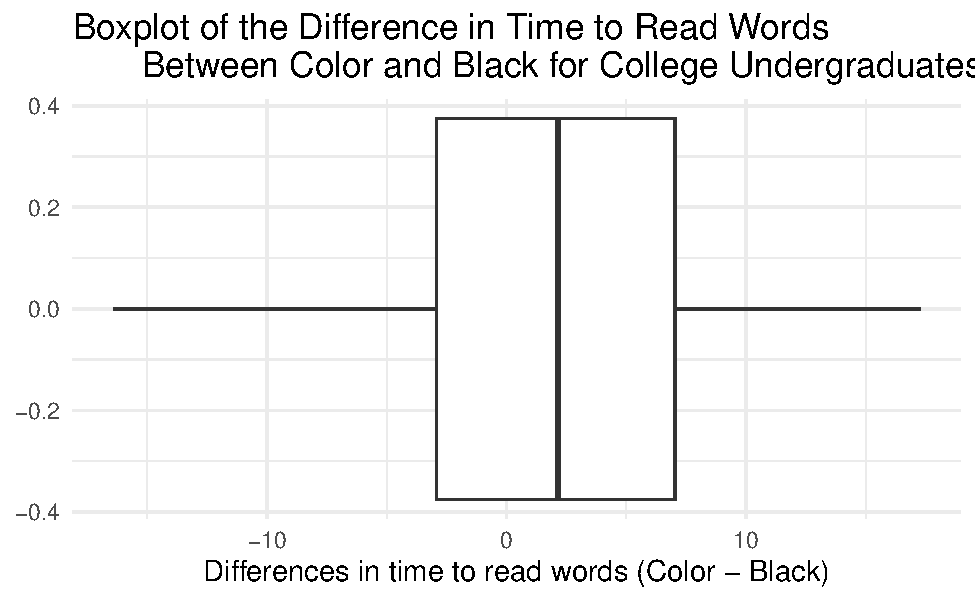
\includegraphics[width=0.7\linewidth]{11-OCA08-paired-theory_files/figure-latex/unnamed-chunk-1-2} \end{center}

The following code gives the summary statistics for the pairwise differences.

\begin{Shaded}
\begin{Highlighting}[]
\NormalTok{color\_diff }\SpecialCharTok{\%\textgreater{}\%} 
  \FunctionTok{summarise}\NormalTok{(}\FunctionTok{favstats}\NormalTok{(differences))}
\CommentTok{\#\textgreater{}      min     Q1 median     Q3   max mean       sd  n missing}
\CommentTok{\#\textgreater{} 1 {-}16.42 {-}2.925   2.15 7.0325 17.27  2.3 7.810196 70       0}
\end{Highlighting}
\end{Shaded}

\hypertarget{check-theoretical-conditions}{%
\subsubsection*{Check theoretical conditions}\label{check-theoretical-conditions}}
\addcontentsline{toc}{subsubsection}{Check theoretical conditions}

\begin{enumerate}
\def\labelenumi{\arabic{enumi}.}
\setcounter{enumi}{3}
\item
  How do you know the independence condition is met for these data?
  \vspace{0.8in}
\item
  Is the normality condition met to use the theory-based methods for analysis? Explain your answer.
  \vspace{1in}
\end{enumerate}

\hypertarget{use-statistical-inferential-methods-to-draw-inferences-from-the-data}{%
\subsubsection*{Use statistical inferential methods to draw inferences from the data}\label{use-statistical-inferential-methods-to-draw-inferences-from-the-data}}
\addcontentsline{toc}{subsubsection}{Use statistical inferential methods to draw inferences from the data}

To find the standardized statistic for the paired differences we will use the following formula:

\[T = \frac{\bar{x}_d - \mu_0}{SE(\bar{x}_d)},\]
where the standard error of the sample mean difference is:

\[SE(\bar{x}_d)=\frac{s_d}{\sqrt{n}}.\]

\begin{enumerate}
\def\labelenumi{\arabic{enumi}.}
\setcounter{enumi}{5}
\tightlist
\item
  Calculate the standard error of the sample mean difference.
\end{enumerate}

\vspace{0.5in}

\begin{enumerate}
\def\labelenumi{\arabic{enumi}.}
\setcounter{enumi}{6}
\tightlist
\item
  How many standard errors is the observed mean difference from the null mean difference?
\end{enumerate}

\vspace{0.5in}

To find the p-value we enter the value for the standardized statistic (T = 2.464) into the pt function in R. If you did not get his answer for question 7, double check your work. For a single sample or paired data, degrees of freedom are found by subtracting 1 from the sample size. You should therefore use \texttt{df} = \(n_d-1 = 70 - 1 = 69\) and \texttt{lower.tail\ =\ FALSE} to find the p-value.

\begin{Shaded}
\begin{Highlighting}[]
\FunctionTok{pt}\NormalTok{(}\FloatTok{2.464}\NormalTok{, }\AttributeTok{df=}\DecValTok{69}\NormalTok{, }\AttributeTok{lower.tail=}\ConstantTok{FALSE}\NormalTok{)}
\CommentTok{\#\textgreater{} [1] 0.008117801}
\end{Highlighting}
\end{Shaded}

\begin{enumerate}
\def\labelenumi{\arabic{enumi}.}
\setcounter{enumi}{7}
\item
  Explain why we found the area above the T-score using \texttt{lower.tail\ =\ FALSE} in the code above.
  \vspace{0.3in}
\item
  What does this p-value mean, in the context of the study? Hint: it is the probability of what\ldots assuming what?
  \vspace{0.8in}
\end{enumerate}

\newpage

To calculate a theory-based confidence interval for the paired mean difference, use the following formula:

\[\bar{x}_d\pm t^* SE(\bar{x}_d).\]
We will need to find the \(t^*\) multiplier using the function \texttt{qt()}. The code below will return the 95th percentile of the \(t\) distribution with \texttt{df} = \(n_d - 1 = 70 - 1 = 69\).

\begin{Shaded}
\begin{Highlighting}[]
\FunctionTok{qt}\NormalTok{(}\FloatTok{0.95}\NormalTok{, }\AttributeTok{df =} \DecValTok{69}\NormalTok{, }\AttributeTok{lower.tail=}\ConstantTok{TRUE}\NormalTok{)}
\CommentTok{\#\textgreater{} [1] 1.667239}
\end{Highlighting}
\end{Shaded}

\begin{figure}

{\centering 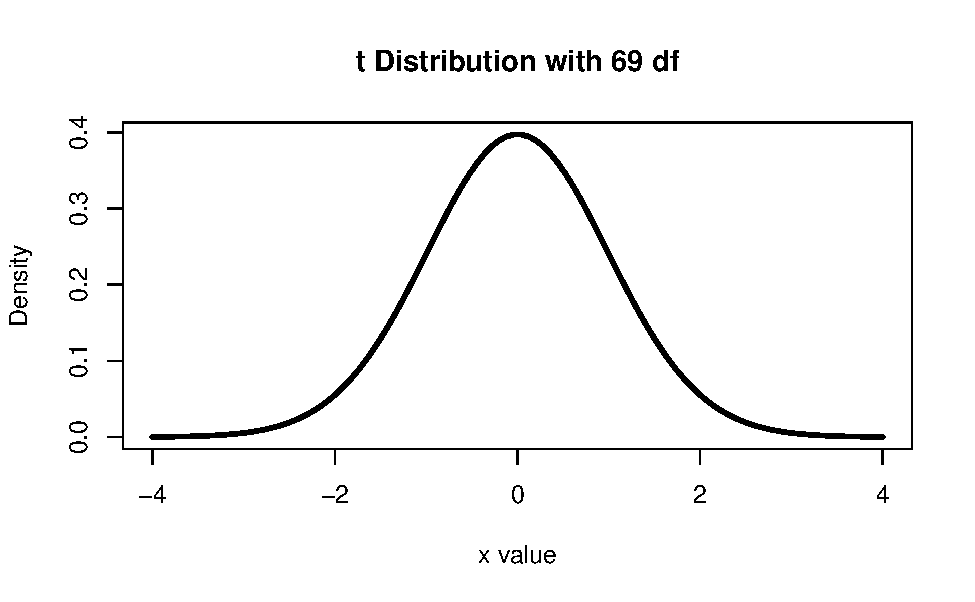
\includegraphics[width=0.7\linewidth]{11-OCA08-paired-theory_files/figure-latex/tstar-1} 

}

\caption{t-distribution with 69 degrees of freedom}\label{fig:tstar}
\end{figure}

\begin{enumerate}
\def\labelenumi{\arabic{enumi}.}
\setcounter{enumi}{9}
\item
  In Figure \ref{fig:tstar}, you see a t-distribution with 69 degrees of freedom. Label \(t^\star\) and \(-t^\star\) on that distribution. Write on the plot the percent of the \(t_{69}\)-distribution that is below \(-t^\star\), between \(-t^\star\) and \(t^\star\), and above \(t^\star\). Then use your plot to determine the confidence level associated with the \(t^\star\) value obtained.
  \vspace{0.3in}
\item
  Calculate the margin of error for the true paired mean difference using theory-based methods.
\end{enumerate}

\vspace{0.6in}

\begin{enumerate}
\def\labelenumi{\arabic{enumi}.}
\setcounter{enumi}{11}
\tightlist
\item
  Calculate the confidence interval for the true paired mean difference using theory-based methods.
\end{enumerate}

\newpage

\begin{enumerate}
\def\labelenumi{\arabic{enumi}.}
\setcounter{enumi}{12}
\tightlist
\item
  Interpret the confidence interval in context of the study.
\end{enumerate}

\vspace{1in}

\begin{enumerate}
\def\labelenumi{\arabic{enumi}.}
\setcounter{enumi}{13}
\tightlist
\item
  Do the results of the CI agree with the p-value? Explain your answer.
\end{enumerate}

\vspace{0.5in}

\begin{enumerate}
\def\labelenumi{\arabic{enumi}.}
\setcounter{enumi}{14}
\tightlist
\item
  Write a conclusion to the test in context of the study.
  \vspace{0.6in}
\end{enumerate}

\hypertarget{take-home-messages-3}{%
\subsection{Take-home messages}\label{take-home-messages-3}}

\begin{enumerate}
\def\labelenumi{\arabic{enumi}.}
\item
  In order to use theory-based methods for dependent groups (paired data), the independent observational units and normality conditions must be met.
\item
  A T-score is compared to a \(t\)-distribution with \(n - 1\) df in order to calculate a one-sided p-value. To find a two-sided p-value using theory-based methods we need to multiply the one-sided p-value by 2.
\item
  A \(t^*\) multiplier is found by obtaining the bounds of the middle X\% (X being the desired confidence level) of a \(t\)-distribution with \(n - 1\) df.
\end{enumerate}

\hypertarget{additional-notes-3}{%
\subsection{Additional notes}\label{additional-notes-3}}

Use this space to summarize your thoughts and take additional notes on today's activity and material covered

\newpage

\hypertarget{activity-11-covid-19-and-air-pollution}{%
\section{Activity 11: COVID-19 and Air Pollution}\label{activity-11-covid-19-and-air-pollution}}

\setstretch{1}

\hypertarget{learning-outcomes-4}{%
\subsection{Learning outcomes}\label{learning-outcomes-4}}

\begin{itemize}
\item
  Given a research question involving paired differences, construct the null and alternative hypotheses
  in words and using appropriate statistical symbols.
\item
  Describe and perform a simulation-based hypothesis test for a paired mean difference.
\item
  Interpret and evaluate a p-value for a simulation-based hypothesis test for a paired mean difference.
\item
  Use bootstrapping to find a confidence interval for a paired mean difference.
\item
  Interpret a confidence interval for a paired mean difference.
\item
  Use a confidence interval to determine the conclusion of a hypothesis test.
\end{itemize}

\hypertarget{terminology-review-3}{%
\subsection{Terminology review}\label{terminology-review-3}}

In today's activity, we will analyze paired quantitative data using simulation-based methods. Some terms covered in this activity are:

\begin{itemize}
\item
  Mean difference
\item
  Paired data
\item
  Independent groups
\item
  Shifted bootstrap (null) distribution
\end{itemize}

To review these concepts, see Section 18 in the textbook.

\hypertarget{covid-19-and-air-pollution}{%
\subsection{COVID-19 and air pollution}\label{covid-19-and-air-pollution}}

In June 2020, the social distancing efforts and stay-at-home directives to help combat the spread of COVID-19 appeared to help `flatten the curve' across the United States, albeit at a high cost to many individuals and businesses. The impact of these measures, though, goes far beyond the infection and death rates from the disease. You may have seen images comparing air quality in large international cities like Rome, Milan, Wuhan, and New Delhi such as the one pictured in Figure \ref{fig:covid}, which seem to indicate, perhaps unsurprisingly, that fewer people driving and factories being shut down have reduced air pollutants.

Have high population-density US cities seen the same improved air quality conditions? To study this question, data were gathered from the US Environmental Protection Agency (EPA) AirData website which records the ozone (O3) and fine particulate matter (PM2.5) values for cities across the US (US Environmental Protection Agency, n.d.). These measures are used to calculate an air quality index (AQI) score for each city each day of the year. Thirty-three of the most densely populated US cities were selected and the AQI score recorded for April 20, 2020 as well as the five-year median AQI score for April 20th (2015--2019). Note that higher AQI scores indicate worse air quality. A box plot of the differences in AQI scores for the 33 cities and a table of summary statistics are shown on the next page. Use Current - 5-year median as the order of subtraction.

\begin{figure}

{\centering 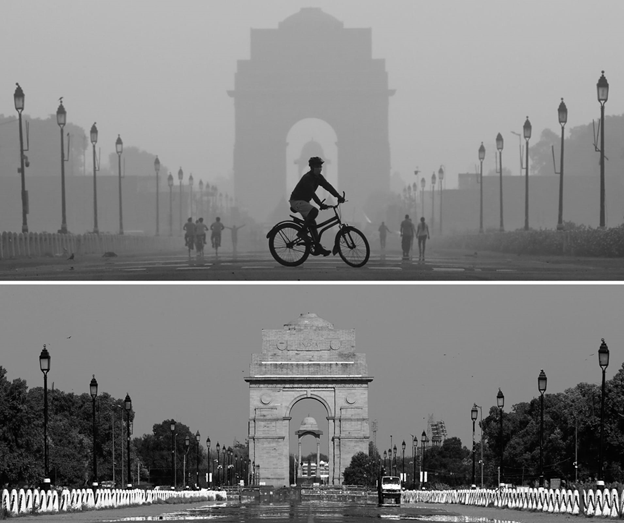
\includegraphics[width=0.6\linewidth]{images/air_pollution_greyscale} 

}

\caption{The India Gate in New Delhi, India.}\label{fig:covid}
\end{figure}

\vspace{.05in}

\begin{center}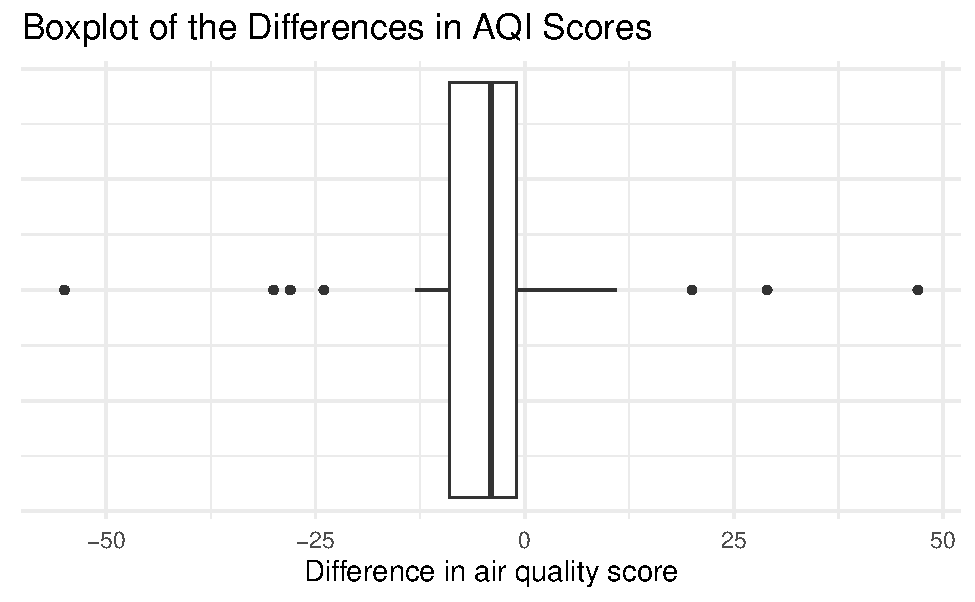
\includegraphics[width=0.6\linewidth]{11-A09-paired-simulation_files/figure-latex/unnamed-chunk-2-1} \end{center}

\vspace{.2in}

\begin{longtable}[]{@{}
  >{\centering\arraybackslash}p{(\columnwidth - 6\tabcolsep) * \real{0.2143}}
  >{\centering\arraybackslash}p{(\columnwidth - 6\tabcolsep) * \real{0.3143}}
  >{\raggedright\arraybackslash}p{(\columnwidth - 6\tabcolsep) * \real{0.2857}}
  >{\raggedright\arraybackslash}p{(\columnwidth - 6\tabcolsep) * \real{0.1857}}@{}}
\caption{Summary statistics for current AQI scores, median AQI scores from 2015--2019, and the differences in AQI scores.}\tabularnewline
\toprule()
\begin{minipage}[b]{\linewidth}\centering
\end{minipage} & \begin{minipage}[b]{\linewidth}\centering
Mean
\end{minipage} & \begin{minipage}[b]{\linewidth}\raggedright
Standard deviation
\end{minipage} & \begin{minipage}[b]{\linewidth}\raggedright
Sample size
\end{minipage} \\
\midrule()
\endfirsthead
\toprule()
\begin{minipage}[b]{\linewidth}\centering
\end{minipage} & \begin{minipage}[b]{\linewidth}\centering
Mean
\end{minipage} & \begin{minipage}[b]{\linewidth}\raggedright
Standard deviation
\end{minipage} & \begin{minipage}[b]{\linewidth}\raggedright
Sample size
\end{minipage} \\
\midrule()
\endhead
Current & \(\bar{x}_1\) = 47.394 & \(s_1\) = 14.107 & \(n_1\) = 33 \\
5 Year Median & \(\bar{x}_2\) = 51.545 & \(s_2\) = 17.447 & \(n_2\) = 33 \\
Differences & \(\bar{x}_d\) = \(-4.152\) & \(s_d\) = 17.096 & \(n_d\) = 33 \\
\bottomrule()
\end{longtable}

\newpage

\hypertarget{vocabulary-review.}{%
\subsubsection*{Vocabulary review.}\label{vocabulary-review.}}
\addcontentsline{toc}{subsubsection}{Vocabulary review.}

\begin{enumerate}
\def\labelenumi{\arabic{enumi}.}
\tightlist
\item
  Identify the variables in this study. What role (explanatory or response) do each have?
\end{enumerate}

\vspace{.5in}

\begin{enumerate}
\def\labelenumi{\arabic{enumi}.}
\setcounter{enumi}{1}
\tightlist
\item
  Are the differences in AQI scores independent for each case (US city)? Explain.
\end{enumerate}

\vspace{0.5in}

\begin{enumerate}
\def\labelenumi{\arabic{enumi}.}
\setcounter{enumi}{2}
\tightlist
\item
  Why is this treated as a paired study design and not two independent samples?
\end{enumerate}

\vspace{0.5in}

\hypertarget{ask-a-research-question-2}{%
\subsubsection*{Ask a research question}\label{ask-a-research-question-2}}
\addcontentsline{toc}{subsubsection}{Ask a research question}

\begin{enumerate}
\def\labelenumi{\arabic{enumi}.}
\setcounter{enumi}{3}
\tightlist
\item
  Write the null hypothesis in words.
\end{enumerate}

\vspace{0.8in}

\begin{enumerate}
\def\labelenumi{\arabic{enumi}.}
\setcounter{enumi}{4}
\tightlist
\item
  What is the research question?
\end{enumerate}

\vspace{0.8in}

\begin{enumerate}
\def\labelenumi{\arabic{enumi}.}
\setcounter{enumi}{5}
\tightlist
\item
  Write the alternative hypothesis in notation.
\end{enumerate}

\vspace{0.3in}

\hypertarget{summarize-and-visualize-the-data-2}{%
\subsubsection*{Summarize and visualize the data}\label{summarize-and-visualize-the-data-2}}
\addcontentsline{toc}{subsubsection}{Summarize and visualize the data}

\begin{enumerate}
\def\labelenumi{\arabic{enumi}.}
\setcounter{enumi}{6}
\tightlist
\item
  Report the summary statistic of interest (mean difference) for the data.
\end{enumerate}

\vspace{0.3in}

\begin{enumerate}
\def\labelenumi{\arabic{enumi}.}
\setcounter{enumi}{7}
\tightlist
\item
  What notation is used for the value in question 7?
\end{enumerate}

\vspace{0.3in}

\hypertarget{use-statistical-inferential-methods-to-draw-inferences-from-the-data-1}{%
\subsubsection*{Use statistical inferential methods to draw inferences from the data}\label{use-statistical-inferential-methods-to-draw-inferences-from-the-data-1}}
\addcontentsline{toc}{subsubsection}{Use statistical inferential methods to draw inferences from the data}

\hypertarget{hypothesis-test}{%
\paragraph*{Hypothesis test}\label{hypothesis-test}}
\addcontentsline{toc}{paragraph}{Hypothesis test}

To simulate the null distribution of paired sample mean differences we will use a bootstrapping method. Recall that the null distribution must be created under the assumption that the null hypothesis is true. Therefore, before bootstrapping, we will need to \emph{shift} each data point by the difference \(\mu_0 - \bar{x}_d\). This will ensure that the mean of the shifted data is \(\mu_0\) (rather than the mean of the original data, \(\bar{x}_d\)), and that the simulated null distribution will be centered at the null value.

\begin{enumerate}
\def\labelenumi{\arabic{enumi}.}
\setcounter{enumi}{8}
\tightlist
\item
  Calculate the difference \(\mu_0 - \bar{x}_d\). Will we need to shift the data up or down?
\end{enumerate}

\vspace{.7in}

We will use the \texttt{paired\_test()} function in R (in the \texttt{catstats} package) to simulate the shifted bootstrap (null) distribution of sample mean differences and compute a p-value. Use the provided R script file and enter the calculated value from question 9 for \texttt{xx} to simulate the null distribution and enter the summary statistic from question 7 for \texttt{yy} to find the p-value. Highlight and run lines 1--21.

\begin{Shaded}
\begin{Highlighting}[]
    \FunctionTok{paired\_test}\NormalTok{(}\AttributeTok{data =}\NormalTok{ Air}\SpecialCharTok{$}\NormalTok{Difference,   }\CommentTok{\# Vector of differences }
                                         \CommentTok{\# or data set with column for each group}
            \AttributeTok{shift =}\NormalTok{ xx,   }\CommentTok{\# Shift needed for bootstrap hypothesis test}
            \AttributeTok{as\_extreme\_as =}\NormalTok{ yy,  }\CommentTok{\# Observed statistic}
            \AttributeTok{direction =} \StringTok{"less"}\NormalTok{,  }\CommentTok{\# Direction of alternative}
            \AttributeTok{number\_repetitions =} \DecValTok{1000}\NormalTok{,  }\CommentTok{\# Number of simulated samples for null distribution}
            \AttributeTok{which\_first =} \DecValTok{1}\NormalTok{)  }\CommentTok{\# Not needed when using calculated differences}
\end{Highlighting}
\end{Shaded}

\begin{enumerate}
\def\labelenumi{\arabic{enumi}.}
\setcounter{enumi}{9}
\tightlist
\item
  Sketch the null distribution created using the R output here.
\end{enumerate}

\vspace{1.8in}

\begin{enumerate}
\def\labelenumi{\arabic{enumi}.}
\setcounter{enumi}{10}
\tightlist
\item
  Explain why the null distribution is centered at zero.
\end{enumerate}

\vspace{.5in}

\begin{enumerate}
\def\labelenumi{\arabic{enumi}.}
\setcounter{enumi}{11}
\item
  What proportion of samples are at or less than the observed sample mean difference in AQI scores for current scores minus 5 year median scores? What is the statistical term for this proportion?
  \vspace{.3in}
\item
  Interpret the p-value in the context of the problem.
  \vspace{.8in}
\item
  How much evidence does this provide for improved air quality in US cities?
  \vspace{.3in}
\item
  If evidence was found for improved air quality in US cities, could we conclude that the stay-at-home directives \emph{caused} the improvement in air quality? Explain.
  \vspace{.5in}
\end{enumerate}

\hypertarget{confidence-interval-3}{%
\paragraph*{Confidence interval}\label{confidence-interval-3}}
\addcontentsline{toc}{paragraph}{Confidence interval}

We will use the \texttt{paired\_bootstrap\_CI()} function in R (in the \texttt{catstats} package) to simulate the bootstrap distribution of sample mean differences and calculate a confidence interval.

\begin{enumerate}
\def\labelenumi{\arabic{enumi}.}
\setcounter{enumi}{15}
\tightlist
\item
  Write out the parameter of interest in context of the study.
\end{enumerate}

\vspace{0.8in}

\begin{enumerate}
\def\labelenumi{\arabic{enumi}.}
\setcounter{enumi}{16}
\tightlist
\item
  Using the provided R script file, fill in the missing value at \texttt{xx} to find a 99\% bootstrap confidence interval; highlight and run lines 24--27. Report the confidence interval in interval notation.
\end{enumerate}

\begin{Shaded}
\begin{Highlighting}[]
\FunctionTok{paired\_bootstrap\_CI}\NormalTok{(}\AttributeTok{data =}\NormalTok{ Air}\SpecialCharTok{$}\NormalTok{Difference, }\CommentTok{\# Enter vector of differences}
                    \AttributeTok{number\_repetitions =} \DecValTok{1000}\NormalTok{, }\CommentTok{\# Number of bootstrap samples for CI}
                    \AttributeTok{confidence\_level =}\NormalTok{ xx,  }\CommentTok{\# Confidence level in decimal form}
                    \AttributeTok{which\_first =} \DecValTok{1}\NormalTok{)  }\CommentTok{\# Not needed when entering vector of differences}
\end{Highlighting}
\end{Shaded}

\vspace{.5in}

\hypertarget{communicate-the-results-and-answer-the-research-question-2}{%
\subsubsection*{Communicate the results and answer the research question}\label{communicate-the-results-and-answer-the-research-question-2}}
\addcontentsline{toc}{subsubsection}{Communicate the results and answer the research question}

\begin{enumerate}
\def\labelenumi{\arabic{enumi}.}
\setcounter{enumi}{17}
\tightlist
\item
  Interpret the 99\% confidence interval in the context of the problem.
\end{enumerate}

\vspace{0.7in}

\begin{enumerate}
\def\labelenumi{\arabic{enumi}.}
\setcounter{enumi}{18}
\tightlist
\item
  Do the results of your confidence interval and hypothesis test agree? What does each tell you about the null hypothesis?
\end{enumerate}

\vspace{.7in}

\hypertarget{take-home-messages-4}{%
\subsection{Take-home messages}\label{take-home-messages-4}}

\begin{enumerate}
\def\labelenumi{\arabic{enumi}.}
\item
  The differences in a paired data set are treated like a single quantitative variable when performing a statistical analysis. Paired data (or paired samples) occur when pairs of measurements are collected. We are only interested in the population (and sample) of differences, and not in the original data.
\item
  When using bootstrapping to create a null distribution centered at the null value for both paired data and a single quantitative variable, we first need to shift the data by the difference \(\mu_0 - \bar{x}_d\), and then sample with replacement from the shifted data.
\item
  When analyzing paired data, the summary statistic is the `mean difference' NOT the `difference in means'\footnote{Technically, if we calculate the differences and then take the mean (mean difference), and we calculate the two means and then take the difference (difference in means), the value will be the same. However, the \emph{sampling variability} of the two statistics will differ, as we will see in Week 12.}. This terminology will be \emph{very} important in interpretations.
\item
  To create one simulated sample on the null distribution for a sample mean or mean difference, shift the original data by adding \((\mu_0 - \bar{x})\) or \((0 - \bar{x}_d)\). Sample with replacement from the shifted data \(n\) times. Calculate and plot the sample mean or the sample mean difference.
\item
  To create one simulated sample on the bootstrap distribution for a sample mean or mean difference, label \(n\) cards with the original response values. Randomly draw with replacement \(n\) times. Calculate and plot the resampled mean or the resampled mean difference.
\end{enumerate}

\hypertarget{additional-notes-4}{%
\subsection{Additional notes}\label{additional-notes-4}}

Use this space to summarize your thoughts and take additional notes on today's activity and material covered.

\newpage

\hypertarget{week-11-lab-swearing}{%
\section{Week 11 Lab: Swearing}\label{week-11-lab-swearing}}

\setstretch{1}

\hypertarget{learning-outcomes-5}{%
\subsection{Learning outcomes}\label{learning-outcomes-5}}

\begin{itemize}
\item
  Identify whether a study is a paired design or independent groups
\item
  Given a research question involving paired data, construct the null and alternative hypotheses
  in words and using appropriate statistical symbols.
\item
  Describe and perform a simulation-based hypothesis test for a mean difference.
\item
  Interpret and evaluate a p-value for a hypothesis test for a mean difference.
\item
  Use bootstrapping methods to find a confidence interval for a mean difference.
\item
  Interpret a confidence interval for a mean difference.
\end{itemize}

\hypertarget{type-of-samples}{%
\subsection{Type of samples}\label{type-of-samples}}

For each of the following scenarios, determine whether the samples are paired or independent.

\begin{enumerate}
\def\labelenumi{\arabic{enumi}.}
\item
  Researchers interested in studying the effect of a medical treatment on insulin rate measured insulin rates of 30 patients before and after the medical treatment.
  \vspace{0.3in}
\item
  \textbf{A university is planning to bring emotional support animals to campus during finals week and wants to determine which type of animals are more effective at calming students. Anxiety levels will be measured before and after each student interacts with either a dog or a cat. The university will then compare change in anxiety levels between the `dog' people and the `cat' people.}
  \vspace{0.3in}
\item
  An industry leader is investigating a possible wage gap between male and non-male employees. Twenty companies within the industry are randomly selected and the average salary for all males and non-males in mid-management positions is recorded for each company.
  \vspace{0.3in}
\end{enumerate}

\hypertarget{swearing}{%
\subsection{Swearing}\label{swearing}}

Profanity (language considered obscene or taboo) and society's attitude about its acceptableness is a highly debated topic, but does swearing serve a physiological purpose or function? Previous research has shown that swearing produces increased heart rates and higher levels of skin conductivity. It is theorized that since swearing provokes intense emotional responses, it acts as a distracter, allowing a person to withstand higher levels of pain. To explore the relationship between swearing and increased pain tolerance, researchers from Keele University (Staffordshire, UK) recruited 83 native English-speaking participants (Stephens and Robertson 2020). Each volunteer performed two trials holding a hand in an ice-water bath, once while repeating the ``f-word'' every three seconds, and once while repeating a neutral word (``table''). The order of the word to repeat was randomly assigned. Researchers recorded the length of time, in seconds, from the moment the participant indicated they were in pain until they removed their hand from the ice water for each trial. They hope to find evidence that pain tolerance is greater (longer times) when a person swears compared to when they say a neutral word, on average. Use Swear -- Neutral as the order of subtraction.

\begin{enumerate}
\def\labelenumi{\arabic{enumi}.}
\setcounter{enumi}{3}
\tightlist
\item
  What does \(\mu_d\) represent in the context of this study?
\end{enumerate}

\vspace{0.8in}

\begin{enumerate}
\def\labelenumi{\arabic{enumi}.}
\setcounter{enumi}{4}
\tightlist
\item
  Write out the null hypothesis in proper notation for this study.
\end{enumerate}

\vspace{0.8in}

\begin{enumerate}
\def\labelenumi{\arabic{enumi}.}
\setcounter{enumi}{5}
\tightlist
\item
  What sign (\(<\), \(>\), or \(\neq\)) would you use in the alternative hypothesis for this study? Explain your choice.
\end{enumerate}

\vspace{0.5in}

Upload and open the R script file for Week 11 lab. Upload and import the csv file, \texttt{pain\_tolerance}. Enter the name of the data set (see the environment tab) for datasetname in the R script file in line 6. Highlight and run lines 1--7 to load the data and create a paired plot of the data.

\begin{Shaded}
\begin{Highlighting}[]
\NormalTok{swearing }\OtherTok{\textless{}{-}}\NormalTok{ datasetname}
\FunctionTok{paired\_observed\_plot}\NormalTok{(swearing)}
\end{Highlighting}
\end{Shaded}

\begin{enumerate}
\def\labelenumi{\arabic{enumi}.}
\setcounter{enumi}{6}
\tightlist
\item
  Based on the plots, does there appear to be some evidence in favor of the alternative hypothesis? How do you know?
  \vspace{0.4in}
\end{enumerate}

Enter the outcome for group 1 (\texttt{Swear}) for \texttt{measurement\_1} and the outcome for group 2 (\texttt{Neutral}) for \texttt{measurement\_2} in line 10. Highlight and run lines 9--12 to get the summary statistics for the data.

\begin{Shaded}
\begin{Highlighting}[]
\NormalTok{swearing\_diff }\OtherTok{\textless{}{-}}\NormalTok{ swearing }\SpecialCharTok{\%\textgreater{}\%} 
  \FunctionTok{mutate}\NormalTok{(}\AttributeTok{differences =}\NormalTok{ measurement\_1 }\SpecialCharTok{{-}}\NormalTok{ measurement\_2)}
\NormalTok{swearing\_diff }\SpecialCharTok{\%\textgreater{}\%} 
    \FunctionTok{summarise}\NormalTok{(}\FunctionTok{favstats}\NormalTok{(differences))}
\end{Highlighting}
\end{Shaded}

\begin{enumerate}
\def\labelenumi{\arabic{enumi}.}
\setcounter{enumi}{7}
\item
  What is the value of \(\bar{x}_d\)? What is the sample size?
  \vspace{0.25in}
\item
  \textbf{How far, on average, is each difference in pain tolerance from the mean of the differences in pain tolerance? What is the appropriate notation for this value?}
\end{enumerate}

\vspace{0.5in}

\hypertarget{use-statistical-inferential-methods-to-draw-inferences-from-the-data-2}{%
\subsection*{Use statistical inferential methods to draw inferences from the data}\label{use-statistical-inferential-methods-to-draw-inferences-from-the-data-2}}
\addcontentsline{toc}{subsection}{Use statistical inferential methods to draw inferences from the data}

\begin{enumerate}
\def\labelenumi{\arabic{enumi}.}
\setcounter{enumi}{9}
\tightlist
\item
  Using the provided graphs and summary statistics, determine if both theory-based methods and simulation methods could be used to analyze the data. Explain your reasoning.
\end{enumerate}

\vspace{0.8in}

\hypertarget{hypothesis-test-1}{%
\subsection*{Hypothesis test}\label{hypothesis-test-1}}
\addcontentsline{toc}{subsection}{Hypothesis test}

Remember that the null distribution is created based on the assumption the null hypothesis is true. In this study, the null hypothesis states that swearing does not affect pain tolerance, or that the length of time a subject kept their hand in the water would be the same whether the patient was swearing or not.

We will use the \texttt{paired\_test()} function in R (in the \texttt{catstats} package) to simulate the null distribution of sample mean differences and compute a p-value.

\begin{enumerate}
\def\labelenumi{\arabic{enumi}.}
\setcounter{enumi}{10}
\tightlist
\item
  When using the \texttt{paired\_test()} function, we need to enter the name of the data set, either the order of subtraction (if the data set has both measurements) or the name of the differences (if the data set contains them). We will also need to provide R with the observed mean difference, the direction of the alternative hypothesis, and the shift required in order to force the null hypothesis to be true. The name of the data set as shown above is \texttt{swearing\_diff} and the column of differences is called \texttt{differences}. What values should be entered for each of the following to create 1000 simulated samples?
\end{enumerate}

\vspace{1mm}

\begin{itemize}
\tightlist
\item
  shift:
\end{itemize}

\vspace{.2in}

\begin{itemize}
\tightlist
\item
  As extreme as:
\end{itemize}

\vspace{.2in}

\begin{itemize}
\tightlist
\item
  Direction (\texttt{"greater"}, \texttt{"less"}, or \texttt{"two-sided"}):
\end{itemize}

\vspace{.2in}

\begin{itemize}
\tightlist
\item
  Number of repetitions:
\end{itemize}

\vspace{.2in}

\begin{enumerate}
\def\labelenumi{\arabic{enumi}.}
\setcounter{enumi}{11}
\tightlist
\item
  Simulate a null distribution and compute the p-value. Using the R script file for this lab, enter your answers for question 11 in place of the \texttt{xx}'s to produce the null distribution with 1000 simulations. Highlight and run lines 15--21.
\end{enumerate}

\begin{Shaded}
\begin{Highlighting}[]
\FunctionTok{paired\_test}\NormalTok{(}\AttributeTok{data =}\NormalTok{ swearing}\SpecialCharTok{$}\NormalTok{differences,   }\CommentTok{\# Vector of differences }
                                 \CommentTok{\# or data set with column for each group}
        \AttributeTok{shift =}\NormalTok{ xx,   }\CommentTok{\# Shift needed for bootstrap hypothesis test}
        \AttributeTok{as\_extreme\_as =}\NormalTok{ xx,  }\CommentTok{\# Observed statistic}
        \AttributeTok{direction =} \StringTok{"xx"}\NormalTok{,  }\CommentTok{\# Direction of alternative}
        \AttributeTok{number\_repetitions =}\NormalTok{ xx,  }\CommentTok{\# Number of simulated samples for null distribution}
        \AttributeTok{which\_first =} \DecValTok{1}\NormalTok{)  }\CommentTok{\# Not needed when using calculated differences}
\end{Highlighting}
\end{Shaded}

~~~~~~~Sketch the null distribution created using the \texttt{paired\_test} code.

\vspace{1.5in}

\hypertarget{communicate-the-results-and-answer-the-research-question-3}{%
\subsection*{Communicate the results and answer the research question}\label{communicate-the-results-and-answer-the-research-question-3}}
\addcontentsline{toc}{subsection}{Communicate the results and answer the research question}

\begin{enumerate}
\def\labelenumi{\arabic{enumi}.}
\setcounter{enumi}{12}
\tightlist
\item
  \textbf{Report the p-value. Based off of this p-value and a 1\% significance level, what decision would you make about the null hypothesis? What potential error might you be making based on that decision?}
\end{enumerate}

\vspace{0.5in}

\begin{enumerate}
\def\labelenumi{\arabic{enumi}.}
\setcounter{enumi}{13}
\tightlist
\item
  Do you expect the 98\% confidence interval to contain the null value of zero? Explain.
\end{enumerate}

\vspace{0.8in}

\hypertarget{confidence-interval-4}{%
\subsection*{Confidence interval}\label{confidence-interval-4}}
\addcontentsline{toc}{subsection}{Confidence interval}

We will use the \texttt{paired\_bootstrap\_CI()} function in R (in the \texttt{catstats} package) to simulate the bootstrap distribution of sample mean differences and calculate a confidence interval.

\begin{enumerate}
\def\labelenumi{\arabic{enumi}.}
\setcounter{enumi}{14}
\tightlist
\item
  Using bootstrapping and the provided R script file, find a 98\% confidence interval. Fill in the missing values/numbers in the \texttt{paired\_bootstrap\_CI()} function to create the 98\% confidence interval. Highlight and run lines 24--27. \textbf{Upload a copy of the bootstrap distribution created to Gradescope for your group.}
\end{enumerate}

\begin{Shaded}
\begin{Highlighting}[]
\FunctionTok{paired\_bootstrap\_CI}\NormalTok{(}\AttributeTok{data =}\NormalTok{ swearing\_diff}\SpecialCharTok{$}\NormalTok{differences, }\CommentTok{\# Enter vector of differences}
                    \AttributeTok{number\_repetitions =} \DecValTok{1000}\NormalTok{, }\CommentTok{\# Number of bootstrap samples for CI}
                    \AttributeTok{confidence\_level =}\NormalTok{ xx,  }\CommentTok{\# Confidence level in decimal form}
                    \AttributeTok{which\_first =} \DecValTok{1}\NormalTok{)  }\CommentTok{\# Not needed when entering vector of differences}
\end{Highlighting}
\end{Shaded}

\newpage

~~~~~~~Sketch the bootstrap distribution created using the code. Report the 98\% confidence interval in interval notation.

\vspace{1.5in}

\begin{enumerate}
\def\labelenumi{\arabic{enumi}.}
\setcounter{enumi}{15}
\tightlist
\item
  Interpret the \emph{confidence level} of the interval you calculated in question 15.
\end{enumerate}

\vspace{0.8in}

\begin{enumerate}
\def\labelenumi{\arabic{enumi}.}
\setcounter{enumi}{16}
\tightlist
\item
  Write a paragraph summarizing the results of this study as if you were describing the results to your roommate. \textbf{Upload a copy of your group's paragraph to Gradescope.} Be sure to describe:
\end{enumerate}

\begin{itemize}
\item
  Summary statistic
\item
  P-value and interpretation
\item
  Conclusion (written to answer the research question)
\item
  Confidence interval and interpretation
\item
  Scope of inference
\end{itemize}

\vspace{2.6in}

\newpage

\hypertarget{inference-for-a-quantitative-response-with-independent-samples}{%
\chapter{Inference for a Quantitative Response with Independent Samples}\label{inference-for-a-quantitative-response-with-independent-samples}}

\hypertarget{module-12-reading-guide-inference-for-a-difference-in-two-means}{%
\section{Module 12 Reading Guide: Inference for a Difference in Two Means}\label{module-12-reading-guide-inference-for-a-difference-in-two-means}}

\hypertarget{chapter-19-inference-for-comparing-two-independent-means}{%
\subsection*{Chapter 19 (Inference for comparing two independent means)}\label{chapter-19-inference-for-comparing-two-independent-means}}
\addcontentsline{toc}{subsection}{Chapter 19 (Inference for comparing two independent means)}

\textbf{Videos}

\begin{itemize}
\tightlist
\item
  19.1
\item
  19.2
\item
  19.3Tests
\item
  19.3Intervals
\end{itemize}

\setstretch{1.25}

\hypertarget{reminders-from-previous-sections-2}{%
\subsubsection*{Reminders from previous sections}\label{reminders-from-previous-sections-2}}
\addcontentsline{toc}{subsubsection}{Reminders from previous sections}

\(n_1\)= sample size of group 1

\(n_2\) = sample size of group 2

\(\overline{x}\) = sample mean

\(s\) = sample standard deviation

\(\mu\) = population mean

\(\sigma\) = population standard deviation

General steps of a hypothesis test:

\begin{enumerate}
\def\labelenumi{\arabic{enumi}.}
\item
  Frame the research question in terms of hypotheses.
\item
  Collect and summarize data using a test statistic.
\item
  Assume the null hypothesis is true, and simulate or mathematically model a null distribution for the test statistic.
\item
  Compare the observed test statistic to the null distribution to calculate a p-value.
\item
  Make a conclusion based on the p-value and write the conclusion in context.
\end{enumerate}

Parameter: a value summarizing a variable(s) for a population.

Statistic: a value summarizing a variable(s) for a sample.

Sampling distribution: plot of statistics from 1000s of samples of the same size taken from the same population.

Standard deviation of a statistic: the variability of statistics from 1000s of samples; how far, on average, each statistic is from the true value of the parameter.

Standard error of a statistic: estimated standard deviation of a statistic.

Hypothesis test: a process to determine how strong the evidence of an effect is. Also called a `significance test'.

Simulation-based method: Simulate lots of samples of size \(n\) under assumption of the null hypothesis, then find the proportion of the simulations that are at least as extreme as the observed sample statistic.

Theory-based method: Develop a mathematical model for the sampling distribution of the statistic under the null hypothesis and use the model to calculate the probability of the observed sample statistic (or one more extreme) occurring.

Null hypothesis (\(H_0\)): the skeptical perspective; no difference; no change; no effect; random chance; what the researcher hopes to prove is \textbf{wrong}.

Alternative hypothesis (\(H_A\)): the new perspective; a difference/increase/decrease; an effect; not random chance; what the researcher hopes to prove is \textbf{correct}.

Null value: the value of the parameter when we assume the null hypothesis is true (labeled as \(parameter_0\)).

Null distribution: the simulated or modeled distribution of statistics (sampling distribution) we would expect to occur if the null hypothesis is true.

P-value: probability of seeing the observed sample data, or something more extreme, assuming the null hypothesis is true.

\(\implies\) Lower the p-value the stronger the evidence AGAINST the null hypothesis and FOR the alternative hypothesis.

Decision: a determination of whether to reject or fail to reject a null hypothesis based on a p-value and a pre-set level of significance.

\begin{itemize}
\item
  If p-value \(\leq \alpha\), then reject \(H_0\).
\item
  If p-value \(> \alpha\), then fail to reject \(H_0\).
\end{itemize}

Significance level (\(\alpha\)): a threshold used to determine if a p-value provides enough evidence to reject the null hypothesis or not.

\rgi Common levels of \(\alpha\) include 0.01, 0.05, and 0.10.

Statistically significant: results are considered statistically significant if the p-value is below the significance level.

Confidence interval: a process to determine how large an effect is; a range of plausible values for the parameter. Also called `estimation'.

Margin of error: the value that is added to and subtracted from the sample statistic to create a confidence interval; half the width of a confidence interval.

Bootstrapping: the process of drawing with replacement \(n\) times from the original sample.

Bootstrapped resample: a random sample of size \(n\) from the original sample, selected with replacement.

Bootstrapped statistic: the statistic recorded from the bootstrapped resample.

Confidence level: how confident we are that the confidence interval will capture the parameter.

Bootstrap \(X\)\% confidence interval: (\((\frac{(1-X)}{2})^{th}\) percentile, \((X+(\frac{(1-X)}{2})^{th}\) percentile) of a bootstrap distribution.

Central Limit Theorem: For large sample sizes, the sampling distribution of a sample mean (or proportion) will be approximately normal (bell-shaped and symmetric).

\(t\)-distribution: A bell-shaped symmetric distribution, centered at 0, wider than the standard normal distribution.

\begin{itemize}
\tightlist
\item
  The variability in a \(t\)-distribution depends on the sample size (used to calculate degrees of freedom --- df for short).
\item
  The \(t\)-distribution gets closer to the standard normal distribution as df increases.
\end{itemize}

Degrees of freedom (df): describes the variability of the \(t\)-distribution.

T-score: the name for a standardized statistic which is compared to a \(t\)-distribution.

\hypertarget{notes-4}{%
\subsubsection*{Notes}\label{notes-4}}
\addcontentsline{toc}{subsubsection}{Notes}

To create a \textbf{simulated null distribution} of differences in independent sample means,

\rgi How many cards will you need and how will the cards be labeled?
\rgs

\rgi What do you do with the cards after labeling them?
\rgs

\rgi After shuffling, what value will be plotted on the simulated null distribution?
\rgs

To create a \textbf{bootstrap distribution} of differences in independent sample means,

\rgi How many cards will you need and how will the cards be labeled?
\rgs

\rgi What do you do with the cards after labeling them?
\rgs

\rgi After shuffling, what value will be plotted on the bootstrap distribution?
\rgs

Conditions to use the CLT for a difference in independent sample means:

\rgi Independence:
\rgs

\rgi \rgi Checked by:
\rgs

\rgi Normality:
\rgs

\rgi \rgi Checked by:
\rgs

In a two-sample \(t\)-test, how are the degrees of freedom determined?
\rgs        

True or false: A large p-value indicates that the null hypothesis is true.
\rgs

\hypertarget{formulas-3}{%
\subsubsection*{Formulas}\label{formulas-3}}
\addcontentsline{toc}{subsubsection}{Formulas}

\(SE(\overline{x_1} - \overline{x_2})=\)
\rgs

\(T=\)
\rgs

Confidence interval for a difference in independent sample means:
\rgs

\hypertarget{notation-2}{%
\subsubsection*{Notation}\label{notation-2}}
\addcontentsline{toc}{subsubsection}{Notation}

\(\mu_1\) represents
\rgs

\(\mu_2\) represents
\rgs

\(\sigma_1\) represents
\rgs

\(\sigma_2\) represents
\rgs

\(\overline{x_1}\) represents
\rgs

\(\overline{x_2}\) represents
\rgs

\(s_1\) represents
\rgs

\(s_2\) represents
\rgs

\hypertarget{example-from-section-19.1-test-scores}{%
\subsubsection*{Example from section 19.1: Test scores}\label{example-from-section-19.1-test-scores}}
\addcontentsline{toc}{subsubsection}{Example from section 19.1: Test scores}

\begin{enumerate}
\def\labelenumi{\arabic{enumi}.}
\item
  What are the observational units?
  \rgs
\item
  What are the sample statistics presented in this example? What notation would be used to represent each value?
  \rgs
\item
  What is the parameter representing in the context of this problem? What notation would be used to represent this parameter?
  \rgs
  \rgs
\item
  What is the research question?
  \rgs
\item
  Write the null and alternative hypothesis in appropriate notation.
  \rgs
\item
  How could we use cards to simulate \textbf{one} sample \emph{which assumes the null hypothesis is true}? How many cards? What is written on the cards? What would we do with the cards? What would you record once you have a simulated sample?
  \rgs
  \rgs
  \rgs
\item
  After 1000 shuffles are generated, where is the resulting simulated distribution centered? Why does that make sense?
  \rgs
  \rgs
\item
  How was the p-value for this test found? The proportion of simulated null samples at \_\_\_\_ or \_\_\_\_\_\_\_\_\_\_\_.
  \rgs
\item
  Interpret the p-value in the context of the problem.
  \rgs
  \rgs
\item
  From these data, can we conclude the exams are equally difficult?
  \rgs
\item
  What type of error may have occurred at the 5\% significance level? Interpret that error in context.
  \rgs
  \rgs
\end{enumerate}

\hypertarget{example-from-section-19.2-esc-and-heart-attacks}{%
\subsubsection*{Example from section 19.2: ESC and heart attacks}\label{example-from-section-19.2-esc-and-heart-attacks}}
\addcontentsline{toc}{subsubsection}{Example from section 19.2: ESC and heart attacks}

\begin{enumerate}
\def\labelenumi{\arabic{enumi}.}
\item
  What is the research question?
  \rgs
\item
  What are the observational units?
  \rgs
\item
  What variables are recorded? Give the type (categorical or quantitative) and role (explanatory or response) of each.
  \rgs
  \rgs
\item
  What are the sample statistics presented in this example? What notation would be used to represent each value?
  \rgs
\item
  What is the parameter representing in the context of this problem? What notation would be used to represent this parameter?
  \rgs
  \rgs
\item
  How could we use cards to simulate \textbf{one} bootstrap resample \emph{which does not assume the null hypothesis is true}? How many cards? What is written on the cards? What would we do with the cards? What would you record once you have a simulated sample?
  \rgs
  \rgs
  \rgs
\item
  After 1000 resamples are generated, where is the resulting bootstrap distribution centered? Why does that make sense?
  \rgs
  \rgs
\item
  Does the 90\% confidence interval provide evidence of a difference across the two treatments?
  \rgs
  \rgs
\end{enumerate}

\hypertarget{example-from-section-19.3-north-carolina-births}{%
\subsubsection*{Example from section 19.3: North Carolina births}\label{example-from-section-19.3-north-carolina-births}}
\addcontentsline{toc}{subsubsection}{Example from section 19.3: North Carolina births}

\begin{enumerate}
\def\labelenumi{\arabic{enumi}.}
\item
  What is the research question?
  \rgs
\item
  What are the observational units?
  \rgs
\item
  What variables will be analyzed? Give the type and role of each.
  \rgs
  \rgs
\item
  Can the results of this study be generalized to a larger population?
  \rgs
\item
  Are causal conclusions appropriate for these data?
  \rgs
\item
  Write the null and the alternative hypotheses in words.
  \rgs
  \rgs
\item
  Write the null and the alternative hypotheses in notation.
  \rgs
\item
  What are the sample statistics presented in this example? What notation would be used to represent each value?
  \rgs
\item
  Are the independence and normality conditions satisfied?
  \rgs
  \rgs
\item
  Calculate the standard error of the difference in sample means.
  \rgs
  \rgs
\item
  Calculate the T-score (the standardized statistic for the sample mean).
  \rgs
  \rgs
\item
  What distribution should the T-score be compared to in order to calculate a p-value?
  \rgs
\item
  What was the p-value of the test?
  \rgs
\item
  What conclusion should the researcher make?
  \rgs
  \rgs
\item
  Calculate a 95\% confidence interval for the parameter of interest using \texttt{qt(0.975,\ df\ =\ 49)\ =\ 1.677} as the \(t^\star\) value.
  \rgs
  \rgs
\item
  Interpret your interval in the context of the problem.
  \rgs
  \rgs
\end{enumerate}

\newpage

\hypertarget{lecture-notes-week-12-inference-for-independent-samples}{%
\section{Lecture Notes Week 12: Inference for independent samples}\label{lecture-notes-week-12-inference-for-independent-samples}}

\setstretch{1}

\hypertarget{single-categorical-single-quantitative-variable-with-independent-samples}{%
\subsection{Single categorical, single quantitative variable with independent samples}\label{single-categorical-single-quantitative-variable-with-independent-samples}}

\setstretch{1.5}

\begin{itemize}
\item
  In this week, we will study inference for a \_\_\_\_\_\_\_\_\_\_\_\_\_\_\_\_\_\_\_\_\_\_ explanatory variable and a \_\_\_\_\_\_\_\_\_\_\_\_\_\_\_\_\_\_\_\_\_\_\_\_\_ response variable where the two groups are \_\_\_\_\_\_\_\_\_\_\_\_\_\_\_\_\_\_\_\_\_\_\_\_\_\_\_\_.
\item
  Independent groups: When the measurements in one sample are not
  \_\_\_\_\_\_\_\_\_\_\_\_\_\_\_\_\_\_\_ to the measurements in the other sample.
\end{itemize}

\setstretch{1}

\begin{itemize}
\item
  Two random samples taken separately from two populations and the same response variable is recorded. Compare the average number of sick days off from work for people who had a flu shot and people who didn't.
\item
  Participants are randomly assigned to one of two treatment conditions, and the same response variable is recorded.
\end{itemize}

Rather than analyzing the differences as a single mean we will calculate summary statistics on each sample.

\setstretch{1.5}

\begin{itemize}
\item
  The summary measure for two independent groups is the \_\_\_\_\_\_\_\_\_\_\_\_\_\_\_\_\_\_\_\_\_\_ in \_\_\_\_\_\_\_\_\_\_\_\_\_\_\_\_\_\_\_\_\_\_\_\_\_\_\_\_\_.
\item
  Difference in means: the difference in average \_\_\_\_\_\_\_\_\_\_\_\_\_\_\_\_\_\_\_\_\_\_\_ variable outcome for observational units between \_\_\_\_\_\_\_\_\_\_\_\_\_\_\_\_\_\_\_\_ variable groups
\end{itemize}

\setstretch{1}

Parameter of Interest:

\begin{itemize}
\item
  Include:

  \begin{itemize}
  \item
    Reference of the population (true, long-run, population, all)
  \item
    Summary measure
  \item
    Context

    \begin{itemize}
    \item
      Observational units/cases
    \item
      Response variable (and explanatory variable if present)

      \begin{itemize}
      \tightlist
      \item
        If the response variable is categorical, define a `success' in context
      \end{itemize}
    \end{itemize}
  \end{itemize}
\end{itemize}

\(\mu_1-\mu_2:\)

\vspace{0.5in}

\setstretch{1.5}

Notation for the Sample Statistics

\begin{itemize}
\item
  Sample mean for group 1:
\item
  Sample mean for group 2:
\item
  Sample difference in means:
\item
  Sample standard deviation for group 1:
\item
  Sample standard deviation for group 2:
\item
  Sample size for group 1:
\item
  Sample size for group 2:
\end{itemize}

\setstretch{1}

Example: Fifty-one (51) college students volunteered to look at impacts on memorization, specifically if putting letters into recognizable patterns (like FBI, CIA, EDA, CDC, etc.) would increase the number letters memorized. The college students were randomly assigned to either a recognizable or non-recognizable letter group. After a period of study time, the number of letters memorized was collect on each study. Is there evidence that putting letters into recognizable letter groups improve memory?

Why should we treat this as two independent groups rather than paired data?

\vspace{0.6in}

Parameter of interest:

\vspace{0.8in}

\begin{Shaded}
\begin{Highlighting}[]
\NormalTok{letters}\OtherTok{\textless{}{-}}\FunctionTok{read.csv}\NormalTok{(}\StringTok{"data/letters.csv"}\NormalTok{)}
\NormalTok{letters }\SpecialCharTok{\%\textgreater{}\%}
    \FunctionTok{reframe}\NormalTok{(}\FunctionTok{favstats}\NormalTok{(Memorized}\SpecialCharTok{\textasciitilde{}}\NormalTok{Grouped))}
\CommentTok{\#\textgreater{}           Grouped min Q1 median    Q3 max     mean       sd  n missing}
\CommentTok{\#\textgreater{} 1 NotRecognizable   1  6     12 14.75  24 11.15385 6.576883 26       0}
\CommentTok{\#\textgreater{} 2    Recognizable   1  6     15 21.00  30 14.32000 8.518216 25       0}
\end{Highlighting}
\end{Shaded}

\begin{Shaded}
\begin{Highlighting}[]
\NormalTok{letters}\SpecialCharTok{\%\textgreater{}\%}
  \FunctionTok{ggplot}\NormalTok{(}\FunctionTok{aes}\NormalTok{(}\AttributeTok{y =}\NormalTok{ Memorized, }\AttributeTok{x =}\NormalTok{ Grouped))  }\SpecialCharTok{+} \CommentTok{\#Enter the name of the explanatory and response variable}
  \FunctionTok{geom\_boxplot}\NormalTok{()}\SpecialCharTok{+}
  \FunctionTok{labs}\NormalTok{(}\AttributeTok{title =} \StringTok{"Boxplot of number of letters memorized by type of grouping"}\NormalTok{, }\CommentTok{\#Title your plot}
       \AttributeTok{y =} \StringTok{"Number of letter memorized"}\NormalTok{, }\CommentTok{\#y{-}axis label}
       \AttributeTok{x =} \StringTok{"Letter Grouping"}\NormalTok{) }\CommentTok{\#x{-}axis label}
\end{Highlighting}
\end{Shaded}

\begin{center}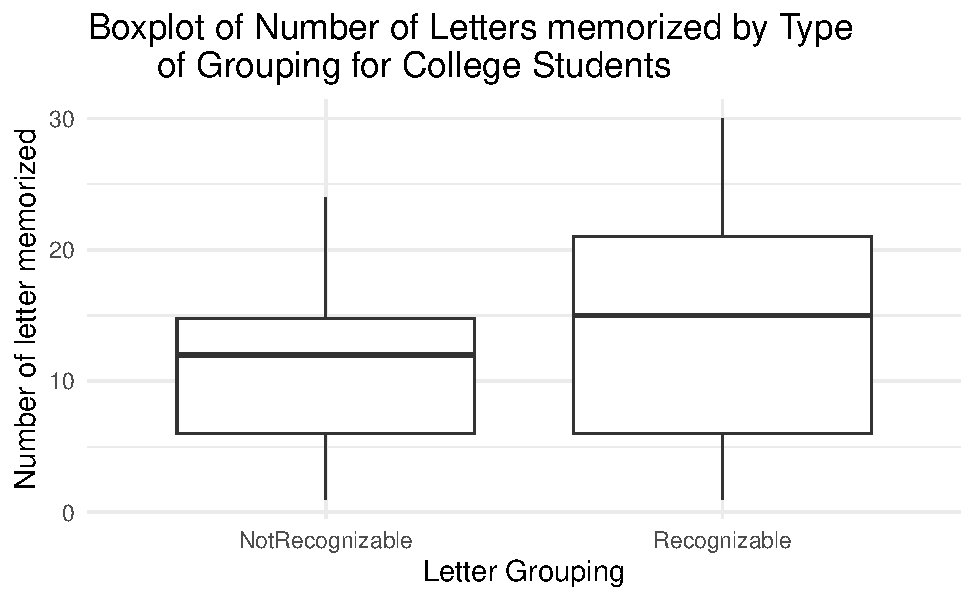
\includegraphics[width=0.7\linewidth]{12-LN012-1ofeach_files/figure-latex/unnamed-chunk-2-1} \end{center}

\hypertarget{hypothesis-testing-4}{%
\subsection*{Hypothesis Testing}\label{hypothesis-testing-4}}
\addcontentsline{toc}{subsection}{Hypothesis Testing}

Conditions:

\begin{itemize}
\tightlist
\item
  Independence:
\end{itemize}

\vspace{0.3in}

Null hypothesis assumes ``no effect'', ``no difference'', ``nothing interesting happening'', etc.

\rgi Always of form: ``parameter'' = null value

\(H_0:\)

\vspace{0.5in}

\(H_A:\)

\vspace{0.5in}

\begin{itemize}
\tightlist
\item
  Research question determines the alternative hypothesis.
\end{itemize}

Write the null and alternative hypotheses for the letters study:

In words:

\(H_0:\)

\vspace{0.5in}

\(H_A:\)

\vspace{0.5in}

In notation:

\(H_0:\)

\vspace{0.2in}

\(H_A:\)

\vspace{0.2in}

\hypertarget{simulation-based-method-5}{%
\subsubsection*{Simulation-based method}\label{simulation-based-method-5}}
\addcontentsline{toc}{subsubsection}{Simulation-based method}

\begin{itemize}
\item
  Simulate many samples assuming \(H_0: \mu_1 = \mu_2\)

  \begin{itemize}
  \item
    Write the response variable values on cards
  \item
    Mix the explanatory variable groups together
  \item
    Shuffle cards into two explanatory variable groups to represent the sample size in each group (\(n_1\) and \(n_2\))
  \item
    Calculate and plot the simulated difference in sample means from each simulation
  \item
    Repeat 1000 times (simulations) to create the null distribution
  \item
    Find the proportion of simulations at least as extreme as \(\bar{x}_1 - \bar{x}_2\)
  \end{itemize}
\end{itemize}

\begin{Shaded}
\begin{Highlighting}[]
\FunctionTok{set.seed}\NormalTok{(}\DecValTok{216}\NormalTok{)}
\FunctionTok{two\_mean\_test}\NormalTok{(Memorized}\SpecialCharTok{\textasciitilde{}}\NormalTok{Grouped, }\CommentTok{\#Enter the names of the variables}
              \AttributeTok{data =}\NormalTok{ letters,  }\CommentTok{\# Enter the name of the dataset}
              \AttributeTok{first\_in\_subtraction =} \StringTok{"Recognizable"}\NormalTok{, }\CommentTok{\# First outcome in order of subtraction}
              \AttributeTok{number\_repetitions =} \DecValTok{1000}\NormalTok{,  }\CommentTok{\# Number of simulations}
              \AttributeTok{as\_extreme\_as =} \FloatTok{3.166}\NormalTok{,  }\CommentTok{\# Observed statistic}
              \AttributeTok{direction =} \StringTok{"greater"}\NormalTok{)  }\CommentTok{\# Direction of alternative: "greater", "less", or "two{-}sided"}
\end{Highlighting}
\end{Shaded}

\begin{center}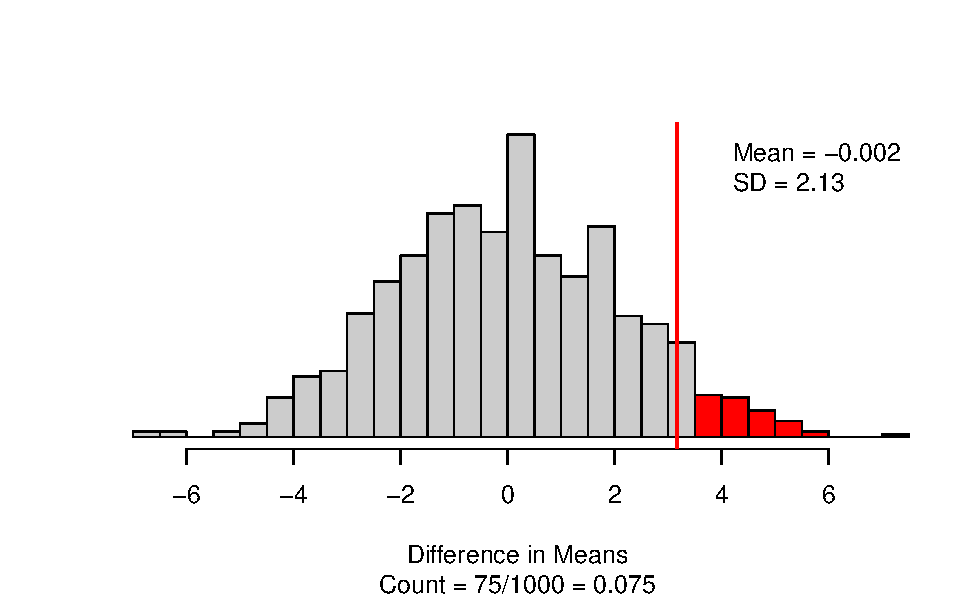
\includegraphics[width=0.7\linewidth]{12-LN012-1ofeach_files/figure-latex/unnamed-chunk-3-1} \end{center}

Explain why the null distribution is centered at the value of zero:

\newpage

Interpretation of the p-value:

\begin{itemize}
\item
  Statement about probability or proportion of samples
\item
  Statistic (summary measure and value)
\item
  Direction of the alternative
\item
  Null hypothesis (in context)
\end{itemize}

\vspace{0.8in}

Conclusion:

\begin{itemize}
\item
  Amount of evidence
\item
  Parameter of interest
\item
  Direction of the alternative hypothesis
\end{itemize}

\vspace{0.6in}

\hypertarget{theory-based-method-4}{%
\subsubsection*{Theory-based method}\label{theory-based-method-4}}
\addcontentsline{toc}{subsubsection}{Theory-based method}

Conditions:

\begin{itemize}
\item
  Independence
\item
  Large enough sample size
\end{itemize}

\vspace{1in}

Like with paired data the t-distribution can be used to model the difference in means.

\setstretch{1.5}

\begin{itemize}
\tightlist
\item
  For a independent samples we use the \_\_\_\_\_\_- distribution
  with \_\_\_\_\_\_\_\_\_\_\_\_\_\_\_\_ degrees of freedom to approximate the sampling distribution.
\end{itemize}

\setstretch{1}

Theory-based test:

\begin{itemize}
\item
  Calculate the standardized statistic
\item
  Find the area under the t-distribution with the smallest \(n - 1\) df {[}min(\(n_1-1, n_2-1\)) at least as extreme as the standardized statistic
\end{itemize}

Equation for the standard error of the difference in sample mean:

\vspace{0.5in}

Equation for the standardized difference in sample mean:

\vspace{0.5in}

Example:

Every year, orange and black monarch butterflies migrate from their summer breeding grounds in the US and Canada to mountain forests in central Mexico, where they hibernate for the winter. Due to abnormal weather patterns and drought affecting monarch habitats and feeding grounds, the population of monarch butterflies is estimated to have decreased by 53\% from the 2018-2019 wintering season to the 2019-2020 wintering season (WWF, 2020). While conservationists often resort to captive-rearing with the goal of raising biologically indistinct individuals for release into the wild, tagging studies have shown that captive-reared monarchs have lower migratory success compared to wild monarchs. For this study, the researchers raised 67 monarchs (descended from wild monarchs) from eggs to maturity and then compared them to a group of 40 wild-caught monarchs. The researchers want to explore whether the maximum grip strength (how many Newtons a butterfly exerts at the moment of release when gently tugged from a mesh-covered perch) differs between captive-reared and wild-caught monarchs. Use Captive -- Wild for order of subtraction.

Write the null and alternative hypotheses in notation.

\(H_0:\)

\vspace{0.2in}

\(H_A:\)

\vspace{0.2in}

\begin{Shaded}
\begin{Highlighting}[]
\NormalTok{butterfly }\OtherTok{\textless{}{-}}\FunctionTok{read.csv}\NormalTok{(}\StringTok{"data/butterfly1.csv"}\NormalTok{)}
\NormalTok{butterflies }\OtherTok{\textless{}{-}}\NormalTok{ butterfly }\SpecialCharTok{\%\textgreater{}\%} 
  \FunctionTok{na.omit}\NormalTok{() }\SpecialCharTok{\%\textgreater{}\%}
  \FunctionTok{rename}\NormalTok{(}\AttributeTok{Monarch\_Group =} \StringTok{"Monarch.Group"}\NormalTok{,}
         \AttributeTok{MaxGrip =} \StringTok{"Max.Grip.Strength..N."}\NormalTok{) }\SpecialCharTok{\%\textgreater{}\%}
  \FunctionTok{mutate}\NormalTok{(}\AttributeTok{Monarch\_Group =} \FunctionTok{factor}\NormalTok{(Monarch\_Group),}
         \AttributeTok{Sex =} \FunctionTok{factor}\NormalTok{(Sex)) }\SpecialCharTok{\%\textgreater{}\%}
  \FunctionTok{mutate}\NormalTok{(}\AttributeTok{Monarch\_Group =} \FunctionTok{fct\_collapse}\NormalTok{(Monarch\_Group,}
               \StringTok{"Captive"} \OtherTok{=} \FunctionTok{c}\NormalTok{(}\StringTok{"Incubator {-} Fall conditions"}\NormalTok{,}
                             \StringTok{"Rearing room {-} summer conditions"}\NormalTok{),}
               \StringTok{"Wild"} \OtherTok{=} \StringTok{"Wild migrants"}\NormalTok{))}

\NormalTok{butterflies }\SpecialCharTok{\%\textgreater{}\%}
    \FunctionTok{reframe}\NormalTok{(}\FunctionTok{favstats}\NormalTok{(MaxGrip}\SpecialCharTok{\textasciitilde{}}\NormalTok{Monarch\_Group))}
\CommentTok{\#\textgreater{}   Monarch\_Group   min    Q1 median     Q3   max      mean         sd  n missing}
\CommentTok{\#\textgreater{} 1       Captive 0.081 0.162  0.217 0.2845 0.596 0.2363731 0.09412948 67       0}
\CommentTok{\#\textgreater{} 2          Wild 0.108 0.271  0.352 0.4330 0.650 0.3607500 0.14066796 40       0}
\end{Highlighting}
\end{Shaded}

\begin{Shaded}
\begin{Highlighting}[]
\NormalTok{butterflies}\SpecialCharTok{\%\textgreater{}\%}
  \FunctionTok{ggplot}\NormalTok{(}\FunctionTok{aes}\NormalTok{(}\AttributeTok{y =}\NormalTok{ MaxGrip, }\AttributeTok{x =}\NormalTok{ Monarch\_Group))  }\SpecialCharTok{+} \CommentTok{\#Enter the name of the explanatory and response variable}
  \FunctionTok{geom\_boxplot}\NormalTok{()}\SpecialCharTok{+}
  \FunctionTok{labs}\NormalTok{(}\AttributeTok{title =} \StringTok{"Boxplot of max grip of Monarch butterflies by environment reared"}\NormalTok{, }\CommentTok{\#Title your plot}
       \AttributeTok{y =} \StringTok{"Max Grip (Newtons)"}\NormalTok{, }\CommentTok{\#y{-}axis label}
       \AttributeTok{x =} \StringTok{"Environment Reared"}\NormalTok{) }\CommentTok{\#x{-}axis label}
\end{Highlighting}
\end{Shaded}

\begin{center}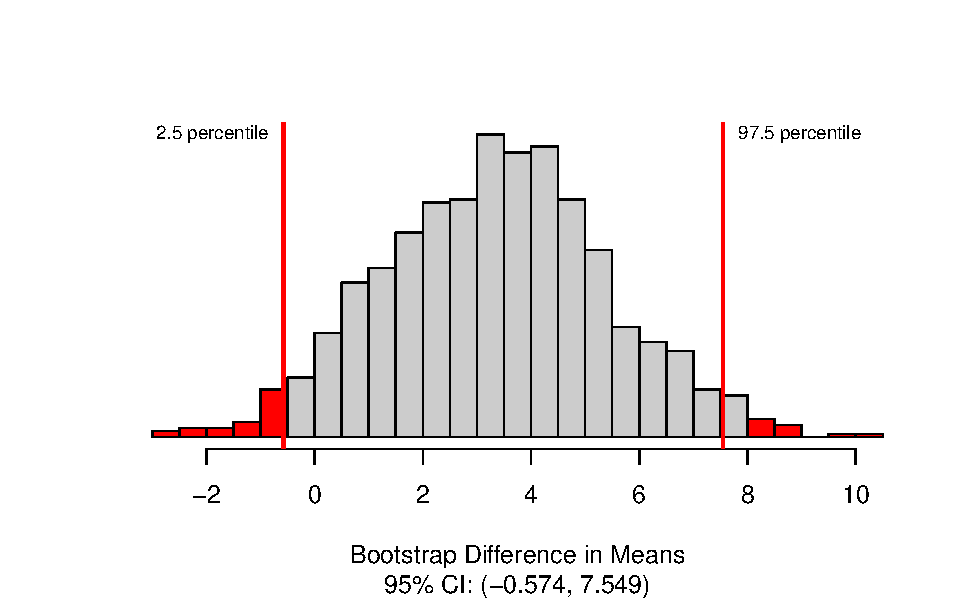
\includegraphics[width=0.7\linewidth]{12-LN012-1ofeach_files/figure-latex/unnamed-chunk-5-1} \end{center}

Are the conditions met to analyze the data using theory based-methods?

\vspace{1in}

Calculate the standardized difference in max grip strength.

\begin{itemize}
\tightlist
\item
  1st calculate the \(SE(\bar{x}_1 - \bar{x}_2)\)
\end{itemize}

\vspace{0.6in}

\begin{itemize}
\tightlist
\item
  Then calculate the T-score
\end{itemize}

\vspace{1in}

\begin{center}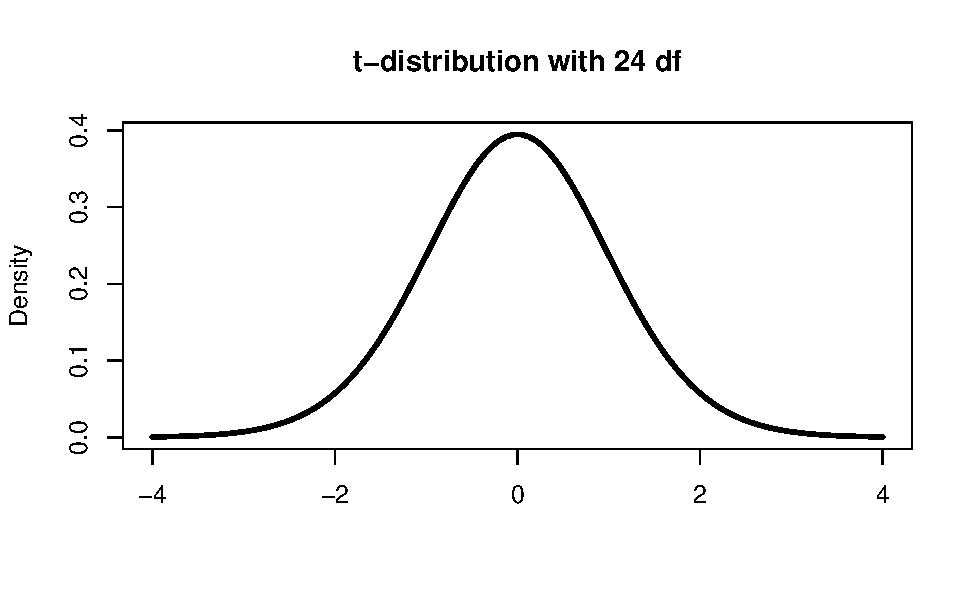
\includegraphics[width=0.7\linewidth]{12-LN012-1ofeach_files/figure-latex/pvaluepb-1} \end{center}

Interpret the standardized statistic:

\vspace{0.8in}

To find the theory-based p-value:

\begin{Shaded}
\begin{Highlighting}[]
\FunctionTok{pt}\NormalTok{(}\SpecialCharTok{{-}}\DecValTok{5}\NormalTok{, }\AttributeTok{df=}\DecValTok{39}\NormalTok{, }\AttributeTok{lower.tail=}\ConstantTok{TRUE}\NormalTok{)}\SpecialCharTok{*}\DecValTok{2}
\CommentTok{\#\textgreater{} [1] 1.252417e{-}05}
\end{Highlighting}
\end{Shaded}

\hypertarget{confidence-interval-5}{%
\subsection*{Confidence interval}\label{confidence-interval-5}}
\addcontentsline{toc}{subsection}{Confidence interval}

To estimate the difference in true mean we will create a confidence interval.

\hypertarget{simulation-based-method-6}{%
\subsubsection*{Simulation-based method}\label{simulation-based-method-6}}
\addcontentsline{toc}{subsubsection}{Simulation-based method}

\begin{itemize}
\item
  Write the response variable values on cards
\item
  Keep explanatory variable groups separate
\item
  Sample with replacement \(n_1\) times in explanatory variable group 1 and \(n_2\) times in explanatory variable group 2
\item
  Calculate and plot the simulated difference in sample means from each simulation
\item
  Repeat 1000 times (simulations) to create the bootstrap distribution
\item
  Find the cut-offs for the middle X\% (confidence level) in a bootstrap distribution.
\end{itemize}

Returning to the letters example, we will estimate the difference in true mean number of letters recognized for students given recognizable letter groupings and students given non-recognizable letter groupings.

\begin{Shaded}
\begin{Highlighting}[]
\FunctionTok{set.seed}\NormalTok{(}\DecValTok{216}\NormalTok{)}
\FunctionTok{two\_mean\_bootstrap\_CI}\NormalTok{(Memorized }\SpecialCharTok{\textasciitilde{}}\NormalTok{ Grouped, }\CommentTok{\#Enter the name of the variables}
                      \AttributeTok{data =}\NormalTok{ letters,  }\CommentTok{\# Enter the name of the data set}
                      \AttributeTok{first\_in\_subtraction =} \StringTok{"Recognizable"}\NormalTok{, }\CommentTok{\# First value in order of subtraction}
                      \AttributeTok{number\_repetitions =} \DecValTok{1000}\NormalTok{,  }\CommentTok{\# Number of simulations}
                      \AttributeTok{confidence\_level =} \FloatTok{0.95}\NormalTok{)}
\end{Highlighting}
\end{Shaded}

\begin{center}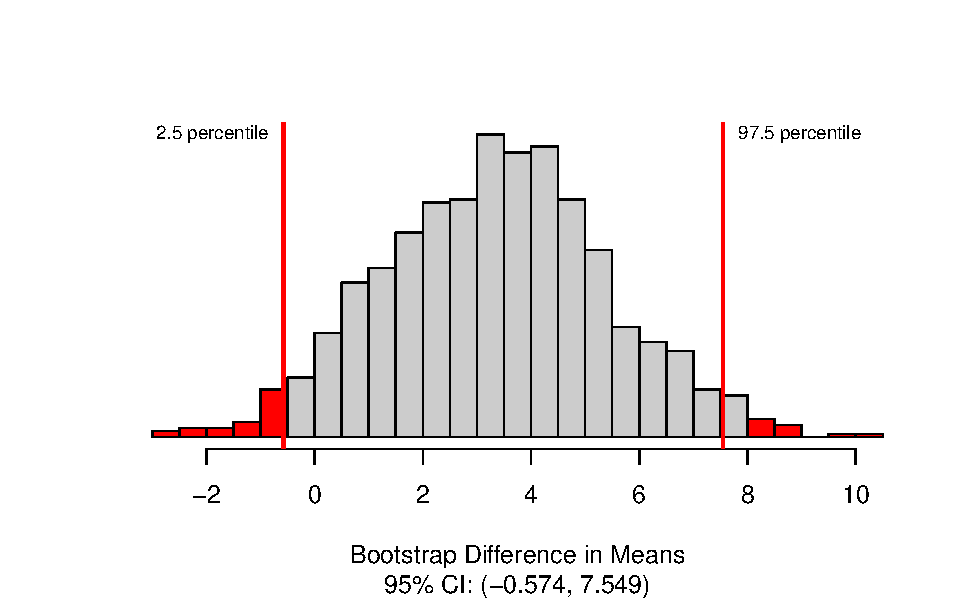
\includegraphics[width=0.7\linewidth]{12-LN012-1ofeach_files/figure-latex/unnamed-chunk-7-1} \end{center}

Confidence interval interpretation:

\begin{itemize}
\item
  How confident you are (e.g., 90\%, 95\%, 98\%, 99\%)
\item
  Parameter of interest
\item
  Calculated interval
\item
  Order of subtraction when comparing two groups
\end{itemize}

\vspace{0.8in}

\hypertarget{theory-based-method-5}{%
\subsubsection*{Theory-based method}\label{theory-based-method-5}}
\addcontentsline{toc}{subsubsection}{Theory-based method}

\begin{itemize}
\tightlist
\item
  Calculate the interval centered at the sample statistic
\end{itemize}

\rgi \(\text{statistic} \pm \text{margin of error}\)

\vspace{0.8in}

Using the Monarch butterfly data, calculate the 99\% confidence interval.

\begin{Shaded}
\begin{Highlighting}[]
\NormalTok{butterflies }\SpecialCharTok{\%\textgreater{}\%}
    \FunctionTok{reframe}\NormalTok{(}\FunctionTok{favstats}\NormalTok{(MaxGrip}\SpecialCharTok{\textasciitilde{}}\NormalTok{Monarch\_Group))}
\CommentTok{\#\textgreater{}   Monarch\_Group   min    Q1 median     Q3   max      mean         sd  n missing}
\CommentTok{\#\textgreater{} 1       Captive 0.081 0.162  0.217 0.2845 0.596 0.2363731 0.09412948 67       0}
\CommentTok{\#\textgreater{} 2          Wild 0.108 0.271  0.352 0.4330 0.650 0.3607500 0.14066796 40       0}
\end{Highlighting}
\end{Shaded}

\begin{itemize}
\tightlist
\item
  Need the \(t^*\) multiplier for a 99\% confidence interval from a t-distribution with \_\_\_\_\_\_\_\_\_ df.
\end{itemize}

\begin{Shaded}
\begin{Highlighting}[]
\FunctionTok{qt}\NormalTok{(}\FloatTok{0.995}\NormalTok{, }\AttributeTok{df=}\DecValTok{39}\NormalTok{, }\AttributeTok{lower.tail =} \ConstantTok{TRUE}\NormalTok{)}
\CommentTok{\#\textgreater{} [1] 2.707913}
\end{Highlighting}
\end{Shaded}

\begin{itemize}
\tightlist
\item
  We will use the same value for the \(SE(\bar{x}_1-\bar{x}_2)\) as calculated for the standardized statistic.
\end{itemize}

\vspace{1in}

Based on the p-value and confidence interval, write a conclusion to the test.

\vspace{1in}
\newpage

\hypertarget{out-of-class-activity-week-12-does-behavior-impact-performance}{%
\section{Out of Class Activity Week 12: Does behavior impact performance?}\label{out-of-class-activity-week-12-does-behavior-impact-performance}}

\setstretch{1}

\hypertarget{learning-outcomes-6}{%
\subsection{Learning outcomes}\label{learning-outcomes-6}}

\begin{itemize}
\item
  Given a research question involving one categorical explanatory variable and one quantitative response variable, construct the null and alternative hypotheses
  in words and using appropriate statistical symbols.
\item
  Describe and perform a simulation-based hypothesis test for a difference in means.
\item
  Interpret and evaluate a p-value for a simulation-based hypothesis test for a difference in means.
\item
  Use bootstrapping to find a confidence interval for a difference in means.
\item
  Interpret a confidence interval for a difference in means.
\item
  Use a confidence interval to determine the conclusion of a hypothesis test.
\end{itemize}

\hypertarget{terminology-review-4}{%
\subsection{Terminology review}\label{terminology-review-4}}

In today's activity, we will use simulation-based methods to analyze the association between one categorical explanatory variable and one quantitative response variable, where the groups formed by the categorical variable are independent. Some terms covered in this activity are:

\begin{itemize}
\item
  Independent groups
\item
  Difference in means
\end{itemize}

To review these concepts, see Chapter 19 in the textbook.

\hypertarget{behavior-and-performance}{%
\subsection{Behavior and Performance}\label{behavior-and-performance}}

A study in the Academy of Management Journal (Porath 2017) investigated how rude behaviors influence a victim's task performance. Randomly selected college students enrolled in a management course were randomly assigned to one of two experimental conditions: rudeness condition (45 students) and control group (53 students). Each student was asked to write down as many uses for a brick as possible in five minutes; this value (total number of uses) was used as a performance measure for each student, where higher values indicate better performance. During this time another individual showed up late for class. For those students in the rudeness condition, the facilitator displayed rudeness by berating the students in general for being irresponsible and unprofessional (due to the late-arriving person). No comments were made about the late-arriving person for students in the control group. Is there evidence that the average performance score for students in the rudeness condition is lower than for students in the control group? Use the order of subtraction of rudeness -- control.

\begin{Shaded}
\begin{Highlighting}[]
\CommentTok{\# Read in data set}
\NormalTok{rude }\OtherTok{\textless{}{-}} \FunctionTok{read.csv}\NormalTok{(}\StringTok{"https://math.montana.edu/courses/s216/data/rude.csv"}\NormalTok{)}
\end{Highlighting}
\end{Shaded}

\newpage

\begin{Shaded}
\begin{Highlighting}[]
\CommentTok{\# Side{-}by{-}side box plots}
\NormalTok{rude }\SpecialCharTok{\%\textgreater{}\%}
\FunctionTok{ggplot}\NormalTok{(}\FunctionTok{aes}\NormalTok{(}\AttributeTok{x =}\NormalTok{ condition, }\AttributeTok{y =}\NormalTok{ number\_of\_uses)) }\SpecialCharTok{+}
    \FunctionTok{geom\_boxplot}\NormalTok{() }\SpecialCharTok{+} 
    \FunctionTok{labs}\NormalTok{(}\AttributeTok{title =} \StringTok{"Number of Uses for a Brick based on Behavior Condition"}\NormalTok{,}
         \AttributeTok{x =} \StringTok{"Behavior"}\NormalTok{) }
\end{Highlighting}
\end{Shaded}

\begin{center}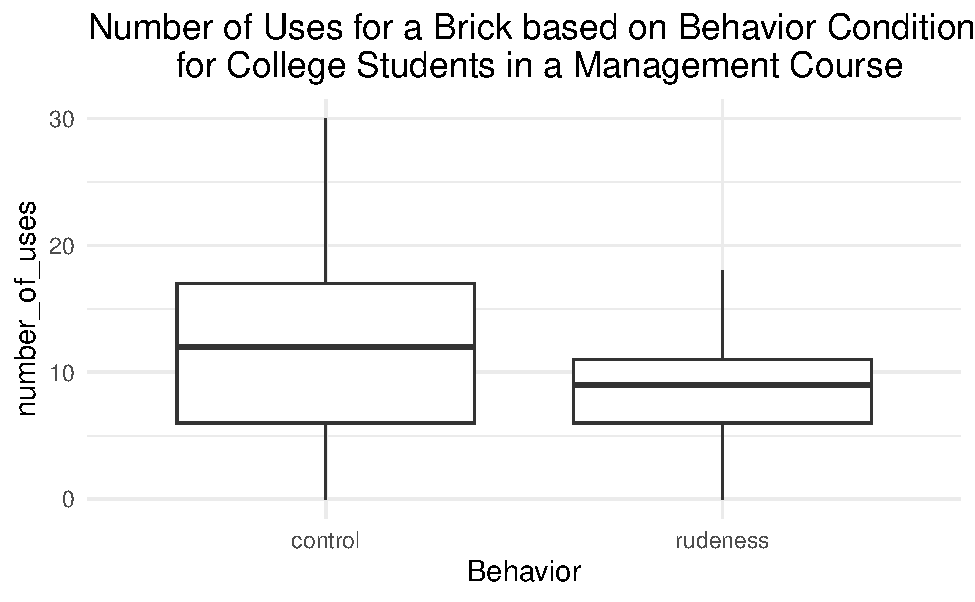
\includegraphics[width=0.6\linewidth]{12-OCA09-inference-1ofeach-simulation_files/figure-latex/unnamed-chunk-2-1} \end{center}

\begin{Shaded}
\begin{Highlighting}[]
\CommentTok{\# Summary statistics}
\NormalTok{rude }\SpecialCharTok{\%\textgreater{}\%} 
     \FunctionTok{reframe}\NormalTok{(}\FunctionTok{favstats}\NormalTok{(number\_of\_uses }\SpecialCharTok{\textasciitilde{}}\NormalTok{ condition))}
\end{Highlighting}
\end{Shaded}

\begin{verbatim}
#>   condition min Q1 median Q3 max      mean       sd  n missing
#> 1   control   0  6     12 17  30 11.811321 7.382559 53       0
#> 2  rudeness   0  6      9 11  18  8.511111 3.992164 45       0
\end{verbatim}

\hypertarget{quantitative-variables-review}{%
\subsubsection*{Quantitative variables review}\label{quantitative-variables-review}}
\addcontentsline{toc}{subsubsection}{Quantitative variables review}

\begin{enumerate}
\def\labelenumi{\arabic{enumi}.}
\tightlist
\item
  The two variables assessed in this study are behavior and number of uses for a brick. Identify the role for each variable (explanatory or response).
\end{enumerate}

\vspace{.4in}

\begin{enumerate}
\def\labelenumi{\arabic{enumi}.}
\setcounter{enumi}{1}
\tightlist
\item
  Which group (control or rudeness) has the highest center in the distributions of number of uses for a brick? Explain which measure of center you are using.
\end{enumerate}

\vspace{.4in}

\begin{enumerate}
\def\labelenumi{\arabic{enumi}.}
\setcounter{enumi}{2}
\tightlist
\item
  Using the side-by-side box plots, which group has the largest spread in number of uses for a brick? How did you make that choice?
\end{enumerate}

\vspace{.4in}

\newpage

\begin{enumerate}
\def\labelenumi{\arabic{enumi}.}
\setcounter{enumi}{3}
\tightlist
\item
  Is this an experiment or an observational study? Justify your answer.
\end{enumerate}

\vspace{1in}

\begin{enumerate}
\def\labelenumi{\arabic{enumi}.}
\setcounter{enumi}{4}
\tightlist
\item
  Is this a paired data set or two independent groups? Explain your reasoning.
\end{enumerate}

\vspace{1in}

\hypertarget{ask-a-research-question-3}{%
\subsubsection*{Ask a research question}\label{ask-a-research-question-3}}
\addcontentsline{toc}{subsubsection}{Ask a research question}

\begin{enumerate}
\def\labelenumi{\arabic{enumi}.}
\setcounter{enumi}{5}
\tightlist
\item
  Write out the parameter of interest in context of the study. Use proper notation and be sure to define your subscripts.
\end{enumerate}

\vspace{1in}

\begin{enumerate}
\def\labelenumi{\arabic{enumi}.}
\setcounter{enumi}{6}
\tightlist
\item
  Write out the null hypothesis in words.
\end{enumerate}

\vspace{1in}

\begin{enumerate}
\def\labelenumi{\arabic{enumi}.}
\setcounter{enumi}{7}
\tightlist
\item
  Write the alternative hypothesis in notation.
\end{enumerate}

\vspace{0.5in}

\hypertarget{summarize-and-visualize-the-data-3}{%
\subsubsection*{Summarize and visualize the data}\label{summarize-and-visualize-the-data-3}}
\addcontentsline{toc}{subsubsection}{Summarize and visualize the data}

\begin{enumerate}
\def\labelenumi{\arabic{enumi}.}
\setcounter{enumi}{8}
\tightlist
\item
  Calculate the summary statistic of interest (difference in means). What is the appropriate notation for this statistic?
\end{enumerate}

\vspace{0.5in}

\newpage

\hypertarget{use-statistical-inferential-methods-to-draw-inferences-from-the-data-3}{%
\subsubsection*{Use statistical inferential methods to draw inferences from the data}\label{use-statistical-inferential-methods-to-draw-inferences-from-the-data-3}}
\addcontentsline{toc}{subsubsection}{Use statistical inferential methods to draw inferences from the data}

\hypertarget{hypothesis-test-2}{%
\paragraph*{Hypothesis test}\label{hypothesis-test-2}}
\addcontentsline{toc}{paragraph}{Hypothesis test}

Remember that the null distribution is created based on the assumption the null hypothesis is true. In this study, the null hypothesis states that there is no association between the two variables. This means that the values observed in the data set would have been the same regardless of the behavior condition.

To demonstrate this simulation, we could create cards to simulate a sample.

\begin{enumerate}
\def\labelenumi{\arabic{enumi}.}
\setcounter{enumi}{9}
\tightlist
\item
  How many cards would we start with?
\end{enumerate}

\vspace{0.3in}

\begin{enumerate}
\def\labelenumi{\arabic{enumi}.}
\setcounter{enumi}{10}
\tightlist
\item
  What would we write on each card?
\end{enumerate}

\vspace{0.3in}

\begin{enumerate}
\def\labelenumi{\arabic{enumi}.}
\setcounter{enumi}{11}
\tightlist
\item
  Next, we would mix the cards together and shuffle into two piles. How many cards will go into each pile? What should we label the piles?
\end{enumerate}

\vspace{.8in}

\begin{enumerate}
\def\labelenumi{\arabic{enumi}.}
\setcounter{enumi}{12}
\tightlist
\item
  What value would be calculated from the cards and plotted on the null distribution? \emph{Hint}: What statistic are we calculating from the data?
\end{enumerate}

\vspace{0.3in}

\begin{enumerate}
\def\labelenumi{\arabic{enumi}.}
\setcounter{enumi}{13}
\tightlist
\item
  Would you expect your simulated statistic to be closer to the null value of zero than the difference in means calculated from the sample? Explain why this makes sense.
\end{enumerate}

\vspace{0.8in}

We will use the \texttt{two\_mean\_test()} function in R (in the \texttt{catstats} package) to simulate the null distribution of differences in sample means and compute a p-value.

\newpage

\begin{enumerate}
\def\labelenumi{\arabic{enumi}.}
\setcounter{enumi}{14}
\tightlist
\item
  When using the \texttt{two\_mean\_test()} function, we need to enter the name of the response variable, \texttt{number\_of\_uses}, and the name of the explanatory variable, \texttt{condition}, for the formula. The name of the data set as shown above is \texttt{rude}. What values should be entered for each of the following to create 1000 simulated samples?
\end{enumerate}

\begin{itemize}
\tightlist
\item
  First in subtraction (What is the outcome for the explanatory variable that is used as first in the order of subtraction? \texttt{"control"} or \texttt{"rudeness"}):
\end{itemize}

\vspace{.2in}

\begin{itemize}
\tightlist
\item
  Number of repetitions:
\end{itemize}

\vspace{.2in}

\begin{itemize}
\tightlist
\item
  As extreme as:
\end{itemize}

\vspace{.2in}

\begin{itemize}
\tightlist
\item
  Direction (\texttt{"greater"}, \texttt{"less"}, or \texttt{"two-sided"}):
\end{itemize}

\vspace{.2in}

The code below will simulate a null distribution and compute the p-value. Check that your answers from question 15 match what is entered below

\begin{Shaded}
\begin{Highlighting}[]
\FunctionTok{set.seed}\NormalTok{(}\DecValTok{216}\NormalTok{)}
\FunctionTok{two\_mean\_test}\NormalTok{(number\_of\_uses}\SpecialCharTok{\textasciitilde{}}\NormalTok{condition, }\CommentTok{\#Enter the names of the variables}
              \AttributeTok{data =}\NormalTok{ rude,  }\CommentTok{\# Enter the name of the dataset}
              \AttributeTok{first\_in\_subtraction =} \StringTok{"rudeness"}\NormalTok{, }\CommentTok{\# First outcome in order of subtraction}
              \AttributeTok{number\_repetitions =} \DecValTok{1000}\NormalTok{,  }\CommentTok{\# Number of simulations}
              \AttributeTok{as\_extreme\_as =} \SpecialCharTok{{-}}\FloatTok{3.3}\NormalTok{,  }\CommentTok{\# Observed statistic}
              \AttributeTok{direction =} \StringTok{"less"}\NormalTok{)  }\CommentTok{\# Direction of alternative: "greater", "less", or "two{-}sided"}
\end{Highlighting}
\end{Shaded}

\begin{center}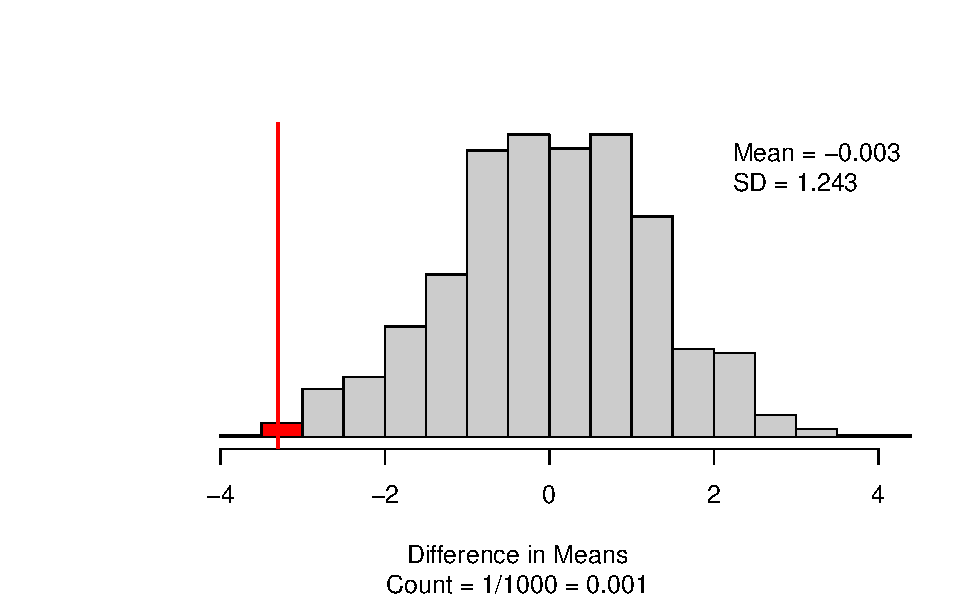
\includegraphics[width=0.7\linewidth]{12-OCA09-inference-1ofeach-simulation_files/figure-latex/unnamed-chunk-4-1} \end{center}

\newpage

\begin{enumerate}
\def\labelenumi{\arabic{enumi}.}
\setcounter{enumi}{15}
\tightlist
\item
  Report the p-value. Based off of this p-value, write a conclusion to the hypothesis test.
\end{enumerate}

\vspace{0.8in}

\hypertarget{confidence-interval-6}{%
\paragraph*{Confidence interval}\label{confidence-interval-6}}
\addcontentsline{toc}{paragraph}{Confidence interval}

We will use the \texttt{two\_mean\_bootstrap\_CI()} function in R (in the \texttt{catstats} package) to simulate the bootstrap distribution of differences in sample means and calculate a 95\% confidence interval.

\begin{Shaded}
\begin{Highlighting}[]
\FunctionTok{set.seed}\NormalTok{(}\DecValTok{216}\NormalTok{)}
\FunctionTok{two\_mean\_bootstrap\_CI}\NormalTok{(number\_of\_uses }\SpecialCharTok{\textasciitilde{}}\NormalTok{ condition, }\CommentTok{\#Enter the name of the variables}
                      \AttributeTok{data =}\NormalTok{ rude,  }\CommentTok{\# Enter the name of the data set}
                      \AttributeTok{first\_in\_subtraction =} \StringTok{"rudeness"}\NormalTok{, }\CommentTok{\# First value in order of subtraction}
                      \AttributeTok{number\_repetitions =} \DecValTok{1000}\NormalTok{,  }\CommentTok{\# Number of simulations}
                      \AttributeTok{confidence\_level =} \FloatTok{0.95}\NormalTok{)}
\end{Highlighting}
\end{Shaded}

\begin{center}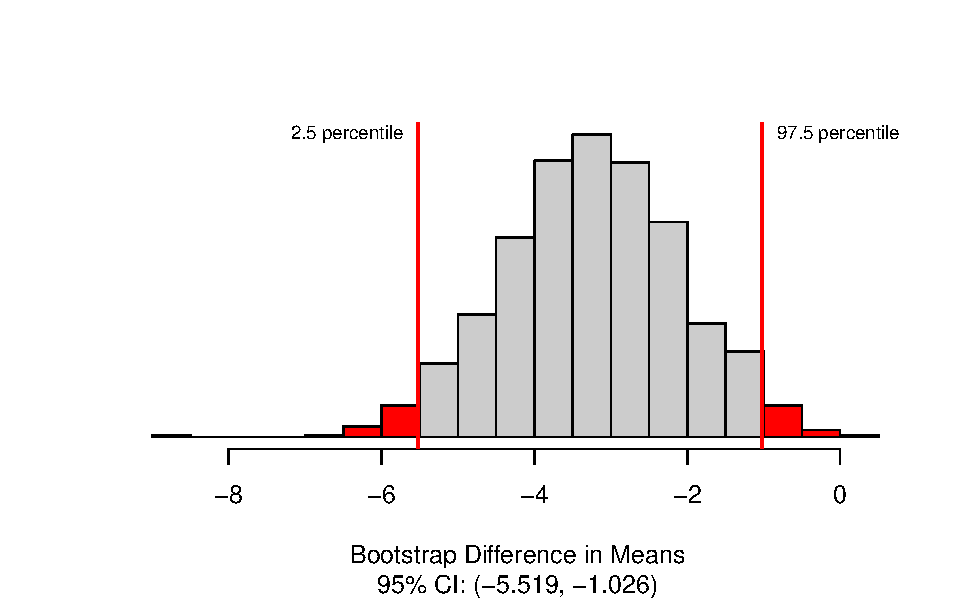
\includegraphics[width=0.7\linewidth]{12-OCA09-inference-1ofeach-simulation_files/figure-latex/unnamed-chunk-5-1} \end{center}

\begin{enumerate}
\def\labelenumi{\arabic{enumi}.}
\setcounter{enumi}{16}
\tightlist
\item
  Report the 95\% confidence interval.
\end{enumerate}

\vspace{0.3in}

\begin{enumerate}
\def\labelenumi{\arabic{enumi}.}
\setcounter{enumi}{17}
\tightlist
\item
  Interpret the interval you calculated in question 17.
\end{enumerate}

\vspace{1in}

\hypertarget{take-home-messages-5}{%
\subsection{Take-home messages}\label{take-home-messages-5}}

\begin{enumerate}
\def\labelenumi{\arabic{enumi}.}
\item
  This activity differs from the activities in Week 11 because the responses are independent, not paired. These data are analyzed as a difference in means, not a mean difference.
\item
  To create one simulated sample on the null distribution for a difference in sample means, label cards with the response variable values from the original data. Mix cards together and shuffle into two new groups of sizes \(n_1\) and \(n_2\). Calculate and plot the difference in means.
\item
  To create one simulated sample on the bootstrap distribution for a difference in sample means, label \(n_1 + n_2\) cards with the original response values. Keep groups separate and randomly draw with replacement \(n_1\) times from group 1 and \(n_2\) times from group 2. Calculate and plot the resampled difference in means.
\end{enumerate}

\hypertarget{additional-notes-5}{%
\subsection{Additional notes}\label{additional-notes-5}}

Use this space to summarize your thoughts and take additional notes on today's activity and material covered

\newpage

\hypertarget{week-12-lab-the-triple-crown}{%
\section{Week 12 Lab: The Triple Crown}\label{week-12-lab-the-triple-crown}}

\setstretch{1}

\hypertarget{learning-outcomes-7}{%
\subsection{Learning outcomes}\label{learning-outcomes-7}}

\begin{itemize}
\item
  Given a research question involving one categorical explanatory variable and one quantitative response variable, construct the null and alternative hypotheses
  in words and using appropriate statistical symbols.
\item
  Describe and perform a theory-based hypothesis test for a difference in means.
\item
  Interpret and evaluate a p-value for a theory-based hypothesis test for a difference in means.
\item
  Use theory-based methods to find a confidence interval for a difference in means.
\item
  Interpret a confidence interval for a difference in means.
\item
  Use a confidence interval to determine the conclusion of a hypothesis test.
\end{itemize}

\hypertarget{terminology-review-5}{%
\subsection{Terminology review}\label{terminology-review-5}}

In today's activity, we will use theory-based methods to analyze the association between one categorical explanatory variable and one quantitative response variable, where the groups formed by the categorical variable are independent. Some terms covered in this activity are:

\begin{itemize}
\item
  Difference in means
\item
  Independence within and between groups
\item
  Normality
\end{itemize}

To review these concepts, see Chapter 19 in the textbook.

\hypertarget{the-triple-crown}{%
\subsection{The triple crown}\label{the-triple-crown}}

The Triple Crown of ``Thru'' hiking consists of hiking the Appalachian Trail, the Pacific Crest Trail (PCT), and the Continental Divide Trail (CDT). Each year halfwayanywhere.com conducts a survey to better understand the people who hike these trails. One variable which is queried in the survey is the pre-hike ``base weight'' of a hiker's pack which is the total weight of gear without food, water, and worn gear. The 131 hikers surveyed who completed the CDT had a mean base weight of 15.266 lbs (sd = 5.128 lbs). The 484 hikers surveyed who completed the PCT had a mean base weight of 17.837 lbs (sd = 7.823 lbs). Is there a difference in average base weight for PCT hikers and CDT hikers? Use order of subtraction CDT - PCT.

\begin{enumerate}
\def\labelenumi{\arabic{enumi}.}
\tightlist
\item
  \textbf{Write out the parameter of interest for this study.}
\end{enumerate}

\vspace{0.8in}

\begin{enumerate}
\def\labelenumi{\arabic{enumi}.}
\setcounter{enumi}{1}
\tightlist
\item
  Write out the null hypothesis in notation for this study. Be sure to clearly identify the subscripts.
\end{enumerate}

\vspace{0.5in}

\begin{enumerate}
\def\labelenumi{\arabic{enumi}.}
\setcounter{enumi}{2}
\tightlist
\item
  Write out the alternative hypothesis in words for this study.
\end{enumerate}

\vspace{0.8in}

The sampling distribution for \(\bar{x}_1-\bar{x}_2\) can be modeled using a normal distribution when certain conditions are met.

Conditions for the sampling distribution of \(\bar{x}_1-\bar{x}_2\) to follow an approximate normal distribution:

\begin{itemize}
\item
  \textbf{Independence}: The sample's observations are independent
\item
  \textbf{Normality}: Each sample should be approximately normal or have a large sample size. For \emph{each} sample:

  \begin{itemize}
  \item
    \(n < 30\): If the sample size \(n\) is less than 30 and there are no clear outliers in the data, then we typically assume the data come from a nearly normal distribution to satisfy the condition.
  \item
    \(n \ge 30\): If the sample size \(n\) is at least 30 and there are no particularly extreme outliers, then we typically assume the sampling distribution of \(\bar{x}\) is nearly normal, even if the underlying distribution of individual observations is not.
  \item
    \(n \geq 100\): If the sample size \(n\) is at least 100 (regardless of the presence of skew or outliers), we typically assume the sampling distribution of \(\bar{x}\) is nearly normal, even if the underlying distribution of individual observations is not.
  \end{itemize}
\end{itemize}

Upload and open the R script file for Week 12 lab. Upload and import the csv file, \texttt{Trail\_Weight}. Enter the name of the data set (see the environment tab) for datasetname in the R script file in line 7. Write a title for the boxplots in line 11. Highlight and run lines 1--13 to load the data and create plots of the data.

\begin{Shaded}
\begin{Highlighting}[]
\NormalTok{hikes }\OtherTok{\textless{}{-}}\NormalTok{ datasetname}
\NormalTok{hikes }\SpecialCharTok{\%\textgreater{}\%}  \CommentTok{\# Data set piped into...}
  \FunctionTok{ggplot}\NormalTok{(}\FunctionTok{aes}\NormalTok{(}\AttributeTok{y =}\NormalTok{ Baseweight, }\AttributeTok{x =}\NormalTok{ Trail))}\SpecialCharTok{+}  \CommentTok{\# Identify variables}
  \FunctionTok{geom\_boxplot}\NormalTok{()}\SpecialCharTok{+}  \CommentTok{\# Tell it to make a box plot}
  \FunctionTok{labs}\NormalTok{(}\AttributeTok{title =} \StringTok{"xx"}\NormalTok{,  }\CommentTok{\# Title}
       \AttributeTok{x =} \StringTok{"Trail"}\NormalTok{,    }\CommentTok{\# x{-}axis label}
       \AttributeTok{y =} \StringTok{"Baseweight(lbs)"}\NormalTok{)  }\CommentTok{\# y{-}axis label}
\end{Highlighting}
\end{Shaded}

\begin{enumerate}
\def\labelenumi{\arabic{enumi}.}
\setcounter{enumi}{3}
\item
  Is the independence condition met? Explain your answer.
  \vspace{0.8in}
\item
  Check that the normality condition is met to use theory-based methods to analyze these data.
\end{enumerate}

\vspace{0.8in}

\newpage

Enter the name of the explanatory variable for \texttt{explanatory} and the name of the response variable for \texttt{response} in line 17. Highlight and run lines 16--17 to get the summary statistics for the data.

\begin{Shaded}
\begin{Highlighting}[]
\NormalTok{hikes }\SpecialCharTok{\%\textgreater{}\%}
  \FunctionTok{summarize}\NormalTok{(}\FunctionTok{favstats}\NormalTok{(response}\SpecialCharTok{\textasciitilde{}}\NormalTok{explanatory))}
\end{Highlighting}
\end{Shaded}

\begin{enumerate}
\def\labelenumi{\arabic{enumi}.}
\setcounter{enumi}{5}
\tightlist
\item
  \textbf{Calculate the summary statistic (difference in means) for this study. Use appropriate notation with clearly defined subscripts.}
\end{enumerate}

\vspace{1in}

\hypertarget{use-statistical-inferential-methods-to-draw-inferences-from-the-data-4}{%
\subsubsection*{Use statistical inferential methods to draw inferences from the data}\label{use-statistical-inferential-methods-to-draw-inferences-from-the-data-4}}
\addcontentsline{toc}{subsubsection}{Use statistical inferential methods to draw inferences from the data}

To find the standardized statistic for the difference in means we will calculate:

\[T = \frac{\bar{x}_1-\bar{x}_2}{SE(\bar{x}_1-\bar{x}_2)},\]

where the standard error of the difference in means is calculated using:

\[SE(\bar{x}_1 -\bar{x}_2)=\sqrt{\frac{s_1^2}{n_1}+\frac{s_2^2}{n_2}}.\]

\begin{enumerate}
\def\labelenumi{\arabic{enumi}.}
\setcounter{enumi}{6}
\tightlist
\item
  Calculate the standard error for the difference in sample means.
\end{enumerate}

\vspace{0.5in}

\begin{enumerate}
\def\labelenumi{\arabic{enumi}.}
\setcounter{enumi}{7}
\tightlist
\item
  \textbf{Calculate the standardized statistic for the difference in sample means.}
\end{enumerate}

\vspace{0.5in}

\begin{enumerate}
\def\labelenumi{\arabic{enumi}.}
\setcounter{enumi}{8}
\tightlist
\item
  When we are comparing two quantitative variables to find the degrees of freedom to use for the t-distribution, we need to use the group with the smallest sample size and subtract 1. (\texttt{df} = minimum of \(n_1 - 1\) or \(n_2 - 1\)). Calculate the \texttt{df} for this study.
\end{enumerate}

\vspace{0.2in}
\newpage

\begin{enumerate}
\def\labelenumi{\arabic{enumi}.}
\setcounter{enumi}{9}
\tightlist
\item
  Using the provided R script file, enter the T-score (for \texttt{xx}) and the \texttt{df} calculated in question 9 for \texttt{yy} into the \texttt{pt()} function to find the p-value. Highlight and run line 20. Report the p-value calculated.
\end{enumerate}

\begin{Shaded}
\begin{Highlighting}[]
\DecValTok{2}\SpecialCharTok{*}\FunctionTok{pt}\NormalTok{(xx, }\AttributeTok{df=}\NormalTok{yy, }\AttributeTok{lower.tail=}\ConstantTok{FALSE}\NormalTok{)}
\end{Highlighting}
\end{Shaded}

\vspace{0.2in}

\begin{enumerate}
\def\labelenumi{\arabic{enumi}.}
\setcounter{enumi}{10}
\item
  \textbf{Explain why we multiplied by 2 in the code above.}
  \vspace{0.3in}
\item
  Do you expect the 95\% confidence interval to contain the null value of zero? Explain your answer.
  \vspace{0.8in}
\end{enumerate}

To calculate a theory-based 95\% confidence interval for a difference in means, use the formula:

\[\bar{x}_1- \bar{x}_2\pm t^* SE(\bar{x}_1- \bar{x}_2).\]

We will need to find the \(t^*\) multiplier using the function \texttt{qt()}. For a 95\% confidence level, we are finding the \(t^*\) value at the 97.5th percentile with (\texttt{df} = minimum of \(n_1 - 1\) or \(n_2 - 1\)).

Enter the appropriate percentile value (as a decimal) for \texttt{xx} and degrees of freedom for \texttt{yy} into the \texttt{qt()} function at line 23 to find the appropriate \(t^*\) multiplier

\begin{Shaded}
\begin{Highlighting}[]
\FunctionTok{qt}\NormalTok{(xx, }\AttributeTok{df =}\NormalTok{ yy, }\AttributeTok{lower.tail=}\ConstantTok{FALSE}\NormalTok{)}
\end{Highlighting}
\end{Shaded}

\begin{enumerate}
\def\labelenumi{\arabic{enumi}.}
\setcounter{enumi}{12}
\tightlist
\item
  Report the \(t^*\) multiplier for the 95\% confidence interval.
\end{enumerate}

\vspace{0.3in}

\begin{enumerate}
\def\labelenumi{\arabic{enumi}.}
\setcounter{enumi}{13}
\tightlist
\item
  Calculate the 95\% confidence interval using theory-based methods.
\end{enumerate}

\vspace{0.5in}

\begin{enumerate}
\def\labelenumi{\arabic{enumi}.}
\setcounter{enumi}{14}
\tightlist
\item
  Do the results of the CI agree with the p-value? Explain your answer.
\end{enumerate}

\vspace{0.5in}

\begin{enumerate}
\def\labelenumi{\arabic{enumi}.}
\setcounter{enumi}{15}
\item
  What type of error may be possible?
  \vspace{0.2in}
\item
  Write a paragraph summarizing the results of the study as if you are reporting the results to your supervisor. \textbf{Upload a copy of your paragraph to Gradescope for your group.} Be sure to describe:
\end{enumerate}

\begin{itemize}
\item
  Summary statistic and interpretation
\item
  P-value and interpretation

  \begin{itemize}
  \item
    Statement about probability or proportion of samples
  \item
    Statistic (summary measure and value)
  \item
    Direction of the alternative
  \item
    Null hypothesis (in context)
  \end{itemize}
\item
  Confidence interval and interpretation

  \begin{itemize}
  \item
    How confident you are (e.g., 90\%, 95\%, 98\%, 99\%)
  \item
    Parameter of interest
  \item
    Calculated interval
  \item
    Order of subtraction when comparing two groups
  \end{itemize}
\item
  Conclusion (written to answer the research question)

  \begin{itemize}
  \item
    Amount of evidence
  \item
    Parameter of interest
  \item
    Direction of the alternative hypothesis
  \end{itemize}
\item
  Scope of inference
\end{itemize}

\newpage

Paragraph:

\newpage

\hypertarget{inference-for-two-quantitative-variables}{%
\chapter{Inference for Two Quantitative Variables}\label{inference-for-two-quantitative-variables}}

\hypertarget{module-13-reading-guide-inference-for-slope-and-correlation}{%
\section{Module 13 Reading Guide: Inference for Slope and Correlation}\label{module-13-reading-guide-inference-for-slope-and-correlation}}

\hypertarget{chapter-21-inference-for-regression-and-model-conditions}{%
\subsection*{Chapter 21 (Inference for regression and model conditions)}\label{chapter-21-inference-for-regression-and-model-conditions}}
\addcontentsline{toc}{subsection}{Chapter 21 (Inference for regression and model conditions)}

\textbf{Videos}

\begin{itemize}
\tightlist
\item
  21.2
\item
  21.3
\item
  21.4to21.5Tests
\item
  21.4to21.5Intervals
\end{itemize}

\setstretch{1.25}

\hypertarget{reminders-from-previous-sections-3}{%
\subsubsection*{Reminders from previous sections}\label{reminders-from-previous-sections-3}}
\addcontentsline{toc}{subsubsection}{Reminders from previous sections}

\(\beta_0\): population \(y\)-intercept

\(\beta_1\): population slope

\(\rho\): population correlation

\(b_0\): sample \(y\)-intercept

\(b_1\): sample slope

\(r\): sample correlation

Scatterplot: displays two quantitative variables; one dot = two measurements (\(x\), \(y\)) on one observational unit.

Four characteristics of a scatterplot:
\setstretch{1}

\begin{itemize}
\tightlist
\item
  \emph{Form}: pattern of the dots plotted. Is the trend generally linear (you can fit a straight line to the data) or non-linear?\\
\item
  \emph{Strength}: how closely do the points follow a trend? Very closely (strong)? No pattern (weak)?\\
\item
  \emph{Direction}: as the \(x\) values increase, do the \(y\)-values tend to increase (positive) or decrease (negative)?\\
\item
  Unusual observations or \emph{outliers}: points that do not fit the overall pattern of the data.
\end{itemize}

\setstretch{1.25}

Least squares regression line: \(\hat{y} = b_0+b_1 \times x\), where \(b_0\) is the sample \(y\)-intercept (the estimate for the \texttt{(Intercept)} row in the R regression output), and \(b_1\) is the sample slope (the estimate for the \texttt{x-variable\_name} row in the R).

Sample slope interpretation: a 1 unit increase in the \emph{x} variable is associated with a \(|b_1|\) unit \emph{predicted} increase/decrease in the \emph{y}-variable.

General steps of a hypothesis test:

\begin{enumerate}
\def\labelenumi{\arabic{enumi}.}
\item
  Frame the research question in terms of hypotheses.
\item
  Collect and summarize data using a test statistic.
\item
  Assume the null hypothesis is true, and simulate or mathematically model a null distribution for the test statistic.
\item
  Compare the observed test statistic to the null distribution to calculate a p-value.
\item
  Make a conclusion based on the p-value and write the conclusion in context.
\end{enumerate}

Parameter: a value summarizing a variable(s) for a population.

Statistic: a value summarizing a variable(s) for a sample.

Sampling distribution: plot of statistics from 1000s of samples of the same size taken from the same population.

Standard deviation of a statistic: the variability of statistics from 1000s of samples; how far, on average, each statistic is from the true value of the parameter.

Standard error of a statistic: estimated standard deviation of a statistic.

Hypothesis test: a process to determine how strong the evidence of an effect is. Also called a `significance test'.

Simulation-based method: Simulate lots of samples of size \(n\) under assumption of the null hypothesis, then find the proportion of the simulations that are at least as extreme as the observed sample statistic.

Theory-based method: Develop a mathematical model for the sampling distribution of the statistic under the null hypothesis and use the model to calculate the probability of the observed sample statistic (or one more extreme) occurring.

Null hypothesis (\(H_0\)): the skeptical perspective; no difference; no change; no effect; random chance; what the researcher hopes to prove is \textbf{wrong}.

Alternative hypothesis (\(H_A\)): the new perspective; a difference/increase/decrease; an effect; not random chance; what the researcher hopes to prove is \textbf{correct}.

Null value: the value of the parameter when we assume the null hypothesis is true (labeled as \(parameter_0\)).

Null distribution: the simulated or modeled distribution of statistics (sampling distribution) we would expect to occur if the null hypothesis is true.

P-value: probability of seeing the observed sample data, or something more extreme, assuming the null hypothesis is true.

\(\implies\) Lower the p-value the stronger the evidence AGAINST the null hypothesis and FOR the alternative hypothesis.

Decision: a determination of whether to reject or fail to reject a null hypothesis based on a p-value and a pre-set level of significance.

\begin{itemize}
\item
  If p-value \(\leq \alpha\), then reject \(H_0\).
\item
  If p-value \(> \alpha\), then fail to reject \(H_0\).
\end{itemize}

Significance level (\(\alpha\)): a threshold used to determine if a p-value provides enough evidence to reject the null hypothesis or not.

\rgi Common levels of \(\alpha\) include 0.01, 0.05, and 0.10.

Statistically significant: results are considered statistically significant if the p-value is below the significance level.

Confidence interval: a process to determine how large an effect is; a range of plausible values for the parameter. Also called `estimation'.

Margin of error: the value that is added to and subtracted from the sample statistic to create a confidence interval; half the width of a confidence interval.

Bootstrapping: the process of drawing with replacement \(n\) times from the original sample.

Bootstrapped resample: a random sample of size \(n\) from the original sample, selected with replacement.

Bootstrapped statistic: the statistic recorded from the bootstrapped resample.

Confidence level: how confident we are that the confidence interval will capture the parameter.

Bootstrap \(X\)\% confidence interval: (\((\frac{(1-X)}{2})^{th}\) percentile, \((X+(\frac{(1-X)}{2})^{th}\) percentile) of a bootstrap distribution

\(t\)-distribution: A bell-shaped symmetric distribution, centered at 0, wider than the standard normal distribution.

\begin{itemize}
\tightlist
\item
  The variability in a \(t\)-distribution depends on the sample size (used to calculate degrees of freedom --- df for short).
\item
  The \(t\)-distribution gets closer to the standard normal distribution as df increases.
\end{itemize}

Degrees of freedom (df): describes the variability of the \(t\)-distribution.

T-score: the name for a standardized statistic which is compared to a \(t\)-distribution.

\hypertarget{notes-5}{%
\subsubsection*{Notes}\label{notes-5}}
\addcontentsline{toc}{subsubsection}{Notes}

To create a \textbf{simulated null distribution} of sample slopes or sample correlations,

\rgi How many cards will you need and how will the cards be labeled?
\rgs

\rgi What do you do with the cards after labeling them?
\rgs

\rgi After shuffling, what value will be plotted on the simulated null distribution?
\rgs

To create a \textbf{bootstrap distribution} of sample slopes or sample correlations,

\rgi How many cards will you need and how will the cards be labeled?
\rgs

\rgi What do you do with the cards after labeling them?
\rgs

\rgi After shuffling, what value will be plotted on the bootstrap distribution?
\rgs

Conditions to use the CLT for testing slope (or correlation):

\rgi Linearity:
\rgs

\rgi \rgi Checked by:
\rgs

\rgi Independent observations:
\rgs

\rgi \rgi Checked by:
\rgs

\rgi Nearly normal residuals:
\rgs

\rgi \rgi Checked by:
\rgs

\rgi Constant or equal variance:
\rgs

\rgi \rgi Checked by:
\rgs

In a theory-based test of slope or correlation, how are the degrees of freedom determined?
\rgs    

Explain why testing for slope is equivalent to testing for correlation.
\rgs

Where in the R output can \(SE(b_1)\) be found?
\rgs

\hypertarget{formulas-4}{%
\subsubsection*{Formulas}\label{formulas-4}}
\addcontentsline{toc}{subsubsection}{Formulas}

\(T=\)
\rgs

Confidence interval:
\rgs

\hypertarget{example-from-sections-21.2-and-21.3-crop-yields}{%
\subsubsection*{Example from sections 21.2 and 21.3: Crop yields}\label{example-from-sections-21.2-and-21.3-crop-yields}}
\addcontentsline{toc}{subsubsection}{Example from sections 21.2 and 21.3: Crop yields}

\begin{enumerate}
\def\labelenumi{\arabic{enumi}.}
\item
  What are the observational units?
  \rgs
\item
  What is the parameter representing in the context of this problem? What notation would be used to represent this parameter?
  \rgs
  \rgs
\item
  What is the research question?
  \rgs
\item
  Write the null and alternative hypotheses in appropriate notation.
  \rgs
\item
  How could we use cards to simulate \textbf{one} sample which assumes \emph{the null hypothesis is true}? How many cards? What is written on the cards? What would we do with the cards? What would you record once you have a simulated sample?
  \rgs
  \rgs
  \rgs
\item
  After 1000 shuffles are generated, where is the resulting simulated distribution centered? Why does that make sense?
  \rgs
  \rgs
\item
  What are the sample statistics presented in this example? What notation would be used to represent each value?
  \rgs
\item
  Write the least squares regression line for these data in appropriate notation.
  \rgs
\item
  How was the p-value for this test found? The proportion of simulated null samples at \_\_\_\_ or \_\_\_\_.
  \rgs
\item
  Interpret the p-value in the context of the problem.
  \rgs
  \rgs
\item
  What conclusion can be drawn from these data?\\
  \rgs
\item
  How could we use cards to simulate \textbf{one} bootstrap resample \emph{which does not assume the null hypothesis is true}? How many cards? What is written on the cards? What would we do with the cards? What would you record once you have a simulated sample?
  \rgs
  \rgs
  \rgs
\item
  Interpret the 95\% confidence interval provided.
  \rgs
  \rgs
\end{enumerate}

\hypertarget{example-from-section-21.4-midterm-elections-and-unemployment}{%
\subsubsection*{Example from section 21.4: Midterm elections and unemployment}\label{example-from-section-21.4-midterm-elections-and-unemployment}}
\addcontentsline{toc}{subsubsection}{Example from section 21.4: Midterm elections and unemployment}

\begin{enumerate}
\def\labelenumi{\arabic{enumi}.}
\item
  What is the research question?
  \rgs
\item
  What are the observational units?
  \rgs
\item
  What variables will be analyzed? Give the type and role of each.
  \rgs
  \rgs
\item
  Can the results of this study be generalized to a larger population?
  \rgs
\item
  Are causal conclusions appropriate for these data?
  \rgs
\item
  Write the null and the alternative hypotheses in words.
  \rgs
  \rgs
\item
  Write the null and the alternative hypotheses in notation.
  \rgs
\item
  What are the sample statistics presented in this example? What notation would be used to represent each value?
  \rgs
\item
  Write the least squares regression line for these data in appropriate notation.
  \rgs
\item
  From the R output provided in table 21.2, what is the standard error of the slope estimate?
  \rgs
\item
  Calculate the T-score (the standardized statistic for the slope).
  \rgs
  \rgs
\item
  What distribution should the T-score be compared to in order to calculate a p-value?
  \rgs
\item
  What was the p-value of the test?
  \rgs
\item
  What conclusion should the researcher make?
  \rgs
  \rgs
\item
  Calculate a 95\% confidence interval for the parameter of interest using \texttt{qt(0.975,\ df\ =\ 27)\ =\ 2.052} as the \(t^\star\) value.
  \rgs
  \rgs
\item
  Interpret your interval in the context of the problem.
  \rgs
  \rgs
\end{enumerate}

\newpage

\hypertarget{lecture-notes-week-13-inference-for-two-quantitative-variable}{%
\section{Lecture Notes Week 13: Inference for two quantitative variable}\label{lecture-notes-week-13-inference-for-two-quantitative-variable}}

\setstretch{1}

\hypertarget{summary-measures-and-plots-for-two-quantitative-variables.}{%
\subsection{Summary measures and plots for two quantitative variables.}\label{summary-measures-and-plots-for-two-quantitative-variables.}}

Scatterplot:

\begin{itemize}
\item
  Form: linear or non-linear?
\item
  Direction: positive or negative?
\item
  Strength: how clear is the pattern between the two variables?
\item
  Outliers: points that are far from the pattern or bulk of the data

  \begin{itemize}
  \tightlist
  \item
    Influential points: outliers that are extreme in the x-~variable.
  \end{itemize}
\end{itemize}

\setstretch{1.5}

The summary measures for two quantitative variables are:

\begin{itemize}
\tightlist
\item
  \_\_\_\_\_\_\_\_\_\_\_\_\_\_\_\_\_\_\_\_\_\_\_\_\_\_\_\_, interpreted as
\end{itemize}

\vspace{0.6in}

\begin{itemize}
\tightlist
\item
  \_\_\_\_\_\_\_\_\_\_\_\_\_\_\_\_\_\_\_\_\_\_\_\_\_\_\_\_, which measures the
\end{itemize}

\vspace{0.6in}

\begin{itemize}
\tightlist
\item
  \_\_\_\_\_\_\_\_\_\_\_\_\_\_\_\_\_\_\_\_\_\_\_\_\_\_\_\_, interpreted as
\end{itemize}

\vspace{0.6in}

\setstretch{1}

\begin{itemize}
\tightlist
\item
  Least-squares regression line: \(\hat{y}=b_0+b_1\times x\) (put y and x in the context of the problem)
\end{itemize}

\setstretch{1.5}

Notation:

\begin{itemize}
\item
  Population slope:
\item
  Population correlation:
\item
  Sample slope:
\item
  Sample correlation:
\end{itemize}

\setstretch{1}

Example: Oceanic temperature is important for sea life. The California Cooperative Oceanic Fisheries Investigations has measured several variables on the Pacific Ocean for more than 70 years hoping to better understand weather patterns and impacts on ocean life. For this example, we will look at the most recent 100 measurements of salt water salinity (measured in PSUs or practical salinity units) and the temperature of the ocean measured in degrees Celsius. Is there evidence that water temperature tends to decrease with higher levels of salinity.

\begin{Shaded}
\begin{Highlighting}[]
\NormalTok{water }\SpecialCharTok{\%\textgreater{}\%} \CommentTok{\# Pipe data set into...}
\FunctionTok{ggplot}\NormalTok{(}\FunctionTok{aes}\NormalTok{(}\AttributeTok{x =}\NormalTok{ Salnty, }\AttributeTok{y =}\NormalTok{ T\_degC))}\SpecialCharTok{+}  \CommentTok{\# Specify variables}
  \FunctionTok{geom\_point}\NormalTok{() }\SpecialCharTok{+}  \CommentTok{\# Add scatterplot of points}
  \FunctionTok{labs}\NormalTok{(}\AttributeTok{x =} \StringTok{"salinity (PSUs)"}\NormalTok{,  }\CommentTok{\# Label x{-}axis}
       \AttributeTok{y =} \StringTok{"temperature (C)"}\NormalTok{,  }\CommentTok{\# Label y{-}axis}
       \AttributeTok{title =} \StringTok{"Scatterplot of Pacific Ocean Salinity vs Temperature"}\NormalTok{) }\SpecialCharTok{+} 
               \CommentTok{\# Be sure to title your plots}
  \FunctionTok{geom\_smooth}\NormalTok{(}\AttributeTok{method =} \StringTok{"lm"}\NormalTok{, }\AttributeTok{se =} \ConstantTok{FALSE}\NormalTok{)  }\CommentTok{\# Add regression line}
\end{Highlighting}
\end{Shaded}

\begin{center}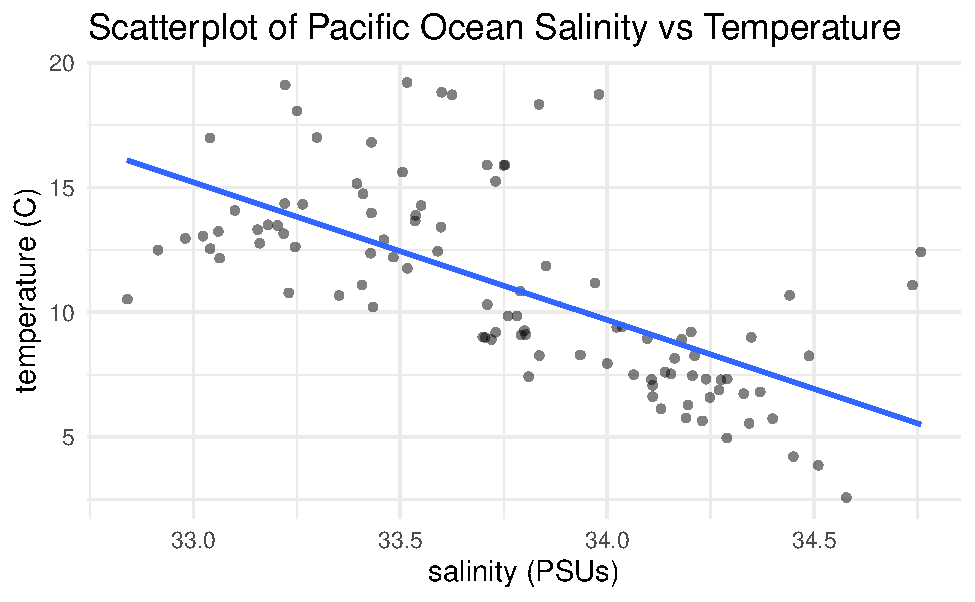
\includegraphics[width=0.7\linewidth]{13-LN013-regression_files/figure-latex/unnamed-chunk-2-1} \end{center}

Describe the four characteristics of the scatterplot:

\vspace{1in}

Linear model output:

\begin{Shaded}
\begin{Highlighting}[]
\NormalTok{lm.water }\OtherTok{\textless{}{-}} \FunctionTok{lm}\NormalTok{(T\_degC}\SpecialCharTok{\textasciitilde{}}\NormalTok{Salnty, }\AttributeTok{data=}\NormalTok{water) }\CommentTok{\# lm(response\textasciitilde{}explanatory)}
\FunctionTok{round}\NormalTok{(}\FunctionTok{summary}\NormalTok{(lm.water)}\SpecialCharTok{$}\NormalTok{coefficients, }\DecValTok{3}\NormalTok{)}
\CommentTok{\#\textgreater{}             Estimate Std. Error t value Pr(\textgreater{}|t|)}
\CommentTok{\#\textgreater{} (Intercept)  197.156     21.478    9.18        0}
\CommentTok{\#\textgreater{} Salnty        {-}5.514      0.636   {-}8.67        0}
\end{Highlighting}
\end{Shaded}

\newpage

Correlation:

\begin{Shaded}
\begin{Highlighting}[]
\FunctionTok{cor}\NormalTok{(T\_degC}\SpecialCharTok{\textasciitilde{}}\NormalTok{Salnty, }\AttributeTok{data=}\NormalTok{water)}
\CommentTok{\#\textgreater{} [1] {-}0.6588365}
\end{Highlighting}
\end{Shaded}

Write the least squares equation of the line in context of the problem:

\vspace{0.5in}

Interpret the value of slope in the context of the problem:

\vspace{0.5in}

Report and describe the correlation value:

\vspace{0.5in}

Calculate and interpret the coefficient of determination:

\vspace{0.8in}

\hypertarget{hypothesis-testing-5}{%
\subsection*{Hypothesis Testing}\label{hypothesis-testing-5}}
\addcontentsline{toc}{subsection}{Hypothesis Testing}

Conditions:

\begin{itemize}
\tightlist
\item
  Independence:
\end{itemize}

\vspace{0.3in}

\begin{itemize}
\tightlist
\item
  Linear relationship:
\end{itemize}

\vspace{0.3in}

Null hypothesis assumes ``no effect'', ``no difference'', ``nothing interesting happening'', etc.

\rgi Always of form: ``parameter'' = null value

\(H_0:\)

\vspace{0.5in}

\(H_A:\)

\vspace{0.5in}

\begin{itemize}
\tightlist
\item
  Research question determines the alternative hypothesis.
\end{itemize}

Write the null and alternative for the ocean study:

In words:

\(H_0:\)

\vspace{0.5in}

\(H_A:\)

\vspace{0.5in}

In notation:

\(H_0:\)

\vspace{0.2in}

\(H_A:\)

\vspace{0.2in}

\hypertarget{simulation-based-method-7}{%
\subsubsection*{Simulation-based method}\label{simulation-based-method-7}}
\addcontentsline{toc}{subsubsection}{Simulation-based method}

\begin{itemize}
\item
  Simulate many samples assuming \(H_0: \beta_1 = 0\) or \(H_0: \rho =0\)

  \begin{itemize}
  \item
    Write the response variable values on cards
  \item
    Hold the explanatory variable values constant
  \item
    Shuffle a new response variable to an explanatory variable
  \item
    Plot the shuffled data points to find the least squares line of regression
  \item
    Calculate and plot the simulated slope or correlation from each simulation
  \item
    Repeat 1000 times (simulations) to create the null distribution
  \item
    Find the proportion of simulations at least as extreme as \(b_1\) or \(r\)
  \end{itemize}
\end{itemize}

To test slope:

\begin{Shaded}
\begin{Highlighting}[]
\FunctionTok{set.seed}\NormalTok{(}\DecValTok{216}\NormalTok{)}
\FunctionTok{regression\_test}\NormalTok{(T\_degC }\SpecialCharTok{\textasciitilde{}}\NormalTok{ Salnty, }\CommentTok{\# response \textasciitilde{} explanatory}
               \AttributeTok{data =}\NormalTok{ water, }\CommentTok{\# Name of data set}
               \AttributeTok{direction =} \StringTok{"less"}\NormalTok{, }\CommentTok{\# Sign in alternative ("greater", "less", "two{-}sided")}
               \AttributeTok{summary\_measure =} \StringTok{"slope"}\NormalTok{, }\CommentTok{\# "slope" or "correlation"}
               \AttributeTok{as\_extreme\_as =} \SpecialCharTok{{-}}\FloatTok{5.514}\NormalTok{, }\CommentTok{\# Observed slope or correlation}
               \AttributeTok{number\_repetitions =} \DecValTok{1000}\NormalTok{) }\CommentTok{\# Number of simulated samples for null distribution}
\end{Highlighting}
\end{Shaded}

\begin{center}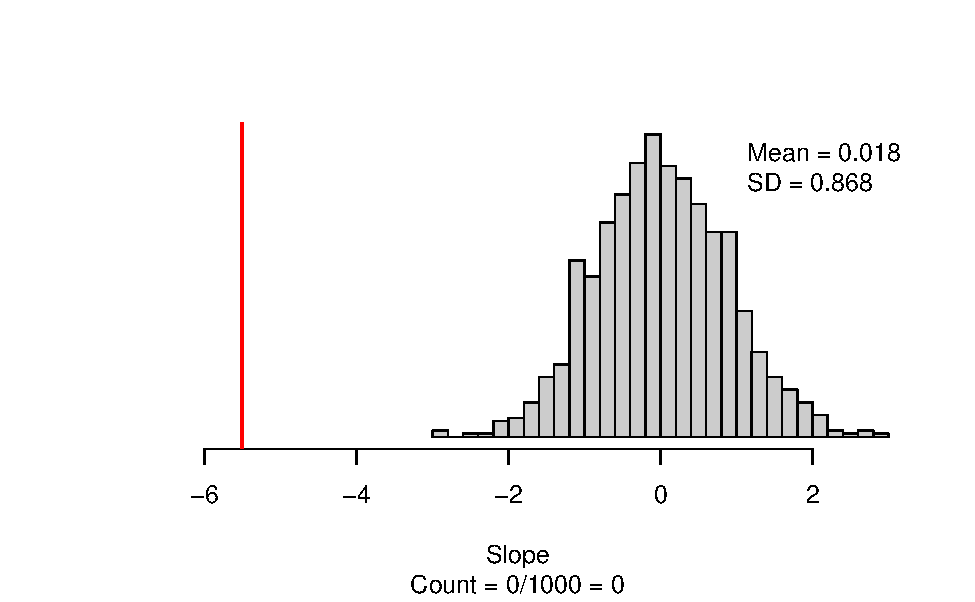
\includegraphics[width=0.7\linewidth]{13-LN013-regression_files/figure-latex/unnamed-chunk-5-1} \end{center}

To test correlation:

\begin{Shaded}
\begin{Highlighting}[]
\FunctionTok{set.seed}\NormalTok{(}\DecValTok{216}\NormalTok{)}
\FunctionTok{regression\_test}\NormalTok{(T\_degC}\SpecialCharTok{\textasciitilde{}}\NormalTok{Salnty, }\CommentTok{\# response \textasciitilde{} explanatory}
               \AttributeTok{data =}\NormalTok{ water, }\CommentTok{\# Name of data set}
               \AttributeTok{direction =} \StringTok{"less"}\NormalTok{, }\CommentTok{\# Sign in alternative ("greater", "less", "two{-}sided")}
               \AttributeTok{summary\_measure =} \StringTok{"correlation"}\NormalTok{, }\CommentTok{\# "slope" or "correlation"}
               \AttributeTok{as\_extreme\_as =} \SpecialCharTok{{-}}\FloatTok{0.659}\NormalTok{, }\CommentTok{\# Observed slope or correlation}
               \AttributeTok{number\_repetitions =} \DecValTok{1000}\NormalTok{) }\CommentTok{\# Number of simulated samples for null distribution}
\end{Highlighting}
\end{Shaded}

\begin{center}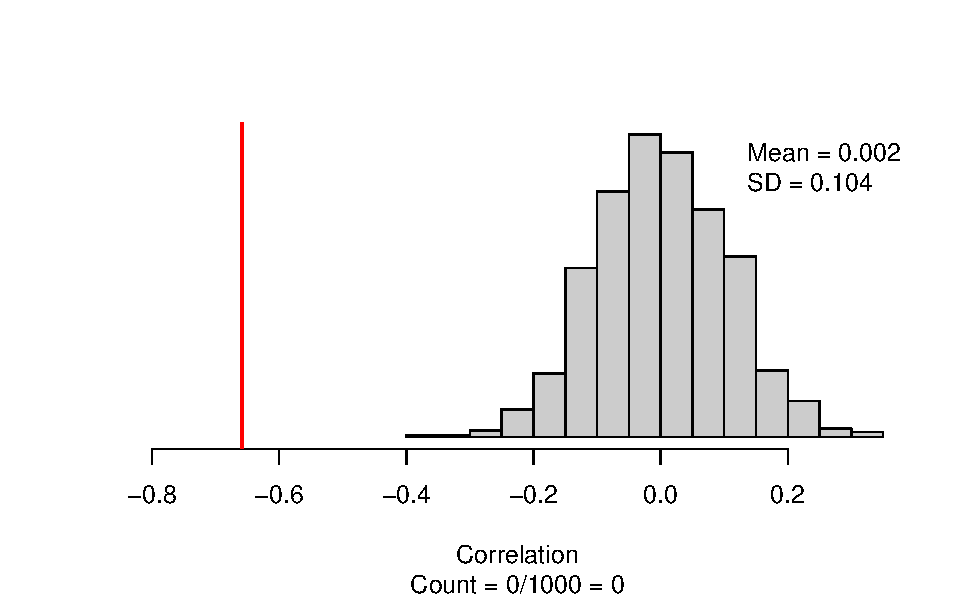
\includegraphics[width=0.7\linewidth]{13-LN013-regression_files/figure-latex/unnamed-chunk-6-1} \end{center}

Explain why the null distribution is centered at the value of zero:

\vspace{0.5in}
\newpage

Interpretation of the p-value:

\begin{itemize}
\item
  Statement about probability or proportion of samples
\item
  Statistic (summary measure and value)
\item
  Direction of the alternative
\item
  Null hypothesis (in context)
\end{itemize}

\vspace{0.8in}

Conclusion:

\begin{itemize}
\item
  Amount of evidence
\item
  Parameter of interest
\item
  Direction of the alternative hypothesis
\end{itemize}

\vspace{0.6in}

\hypertarget{theory-based-method-6}{%
\subsubsection*{Theory-based method}\label{theory-based-method-6}}
\addcontentsline{toc}{subsubsection}{Theory-based method}

Conditions:

\setstretch{1.5}

\begin{itemize}
\item
  Linearity (for both simulation-based and theory-based methods): the data should follow a linear trend.

  \begin{itemize}
  \tightlist
  \item
    Check this assumption by examining the \_\_\_\_\_\_\_\_\_\_\_\_\_\_\_\_\_\_\_\_\_\_\_\_\_\_\_\_ of the two variables, and \_\_\_\_\_\_\_\_\_\_\_\_\_\_\_\_\_\_\_\_\_\_\_\_\_\_\_\_\_\_\_\_\_\_\_\_\_\_\_\_\_\_\_\_. The pattern in the residual plot should display a horizontal line.
  \end{itemize}
\item
  Independence (for both simulation-based and theory-based methods)

  \begin{itemize}
  \tightlist
  \item
    One\_\_\_\_\_\_\_\_\_\_\_\_\_\_\_\_\_\_\_\_\_\_\_\_\_\_\_\_\_\_for an observational unit has no impact on \_\_\_\_\_\_\_\_\_\_\_\_\_\_\_\_\_\_\_\_\_\_\_\_\_\_\_\_\_\_\_\_.
  \end{itemize}
\item
  Constant variability (for theory-based methods only): the variability of points around the least squares line remains roughly constant

  \begin{itemize}
  \tightlist
  \item
    Check this assumption by examining the \_\_\_\_\_\_\_\_\_\_\_\_\_\_\_\_\_\_\_\_\_\_\_\_\_\_\_\_\_\_\_\_. The variability in the residuals around zero should be approximately the same for all fitted values.
  \end{itemize}
\end{itemize}

\newpage

\begin{itemize}
\item
  Nearly normal residuals (for theory-based methods only): residuals must be nearly normal

  \begin{itemize}
  \tightlist
  \item
    Check this assumption by examining a \_\_\_\_\_\_\_\_\_\_\_\_\_\_\_\_\_\_\_\_\_\_\_\_\_\_\_\_\_\_\_\_\_, which should appear approximately normal
  \end{itemize}
\end{itemize}

\setstretch{1}

Example:

It is a generally accepted fact that the more carats a diamond has, the more expensive that diamond will be. The question is, how much more expensive? Data on thousands of diamonds were collected for this data set. We will only look at one type of cut (``Ideal'') and diamonds less than 1 carat. Does the association between carat size and price have a linear relationship for these types of diamonds? What can we state about the association between carat size and price?

Scatterplot:

\begin{Shaded}
\begin{Highlighting}[]
\NormalTok{Diamonds }\SpecialCharTok{\%\textgreater{}\%} \CommentTok{\# Pipe data set into...}
    \FunctionTok{ggplot}\NormalTok{(}\FunctionTok{aes}\NormalTok{(}\AttributeTok{x =}\NormalTok{ carat, }\AttributeTok{y =}\NormalTok{ price))}\SpecialCharTok{+}  \CommentTok{\# Specify variables}
    \FunctionTok{geom\_point}\NormalTok{() }\SpecialCharTok{+}  \CommentTok{\# Add scatterplot of points}
    \FunctionTok{labs}\NormalTok{(}\AttributeTok{x =} \StringTok{"carat"}\NormalTok{,  }\CommentTok{\# Label x{-}axis}
       \AttributeTok{y =} \StringTok{"price ($)"}\NormalTok{,  }\CommentTok{\# Label y{-}axis}
       \AttributeTok{title =} \StringTok{"Scatterplot of Diamonds Carats vs Price"}\NormalTok{) }\SpecialCharTok{+} 
               \CommentTok{\# Be sure to title your plots}
    \FunctionTok{geom\_smooth}\NormalTok{(}\AttributeTok{method =} \StringTok{"lm"}\NormalTok{, }\AttributeTok{se =} \ConstantTok{FALSE}\NormalTok{)  }\CommentTok{\# Add regression line}
\end{Highlighting}
\end{Shaded}

\begin{center}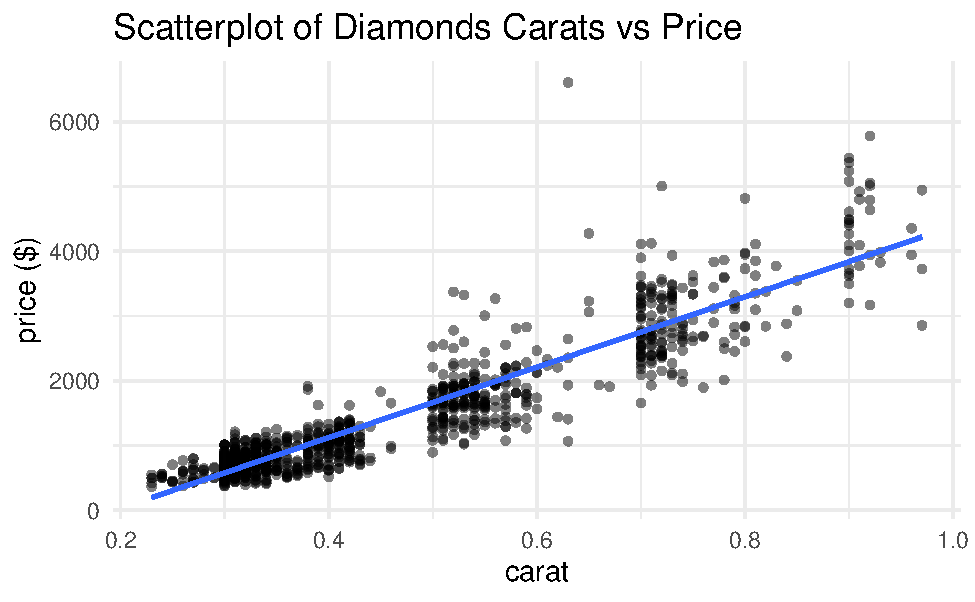
\includegraphics[width=0.7\linewidth]{13-LN013-regression_files/figure-latex/unnamed-chunk-8-1} \end{center}
\newpage

Diagnostic plots:

\begin{center}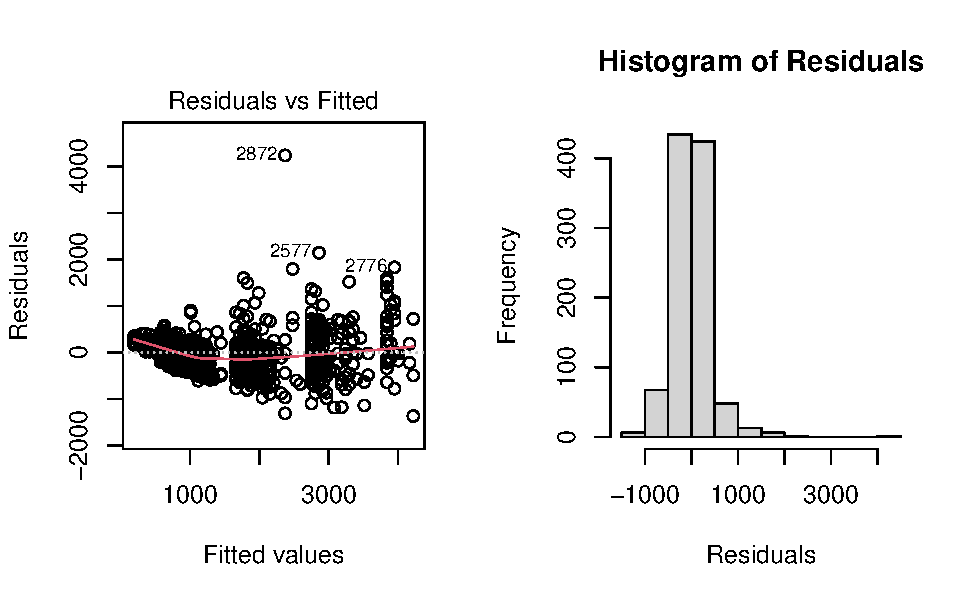
\includegraphics[width=0.7\linewidth]{13-LN013-regression_files/figure-latex/unnamed-chunk-9-1} \end{center}

Check the conditions for the ocean data:

Scatterplot:

\begin{Shaded}
\begin{Highlighting}[]
\NormalTok{water }\SpecialCharTok{\%\textgreater{}\%} \CommentTok{\# Pipe data set into...}
\FunctionTok{ggplot}\NormalTok{(}\FunctionTok{aes}\NormalTok{(}\AttributeTok{x =}\NormalTok{ Salnty, }\AttributeTok{y =}\NormalTok{ T\_degC))}\SpecialCharTok{+}  \CommentTok{\# Specify variables}
  \FunctionTok{geom\_point}\NormalTok{() }\SpecialCharTok{+}  \CommentTok{\# Add scatterplot of points}
  \FunctionTok{labs}\NormalTok{(}\AttributeTok{x =} \StringTok{"salinity (PSUs)"}\NormalTok{,  }\CommentTok{\# Label x{-}axis}
       \AttributeTok{y =} \StringTok{"temperature (C)"}\NormalTok{,  }\CommentTok{\# Label y{-}axis}
       \AttributeTok{title =} \StringTok{"Scatterplot of Pacific Ocean Salinity vs Temperature"}\NormalTok{) }\SpecialCharTok{+} 
               \CommentTok{\# Be sure to title your plots}
  \FunctionTok{geom\_smooth}\NormalTok{(}\AttributeTok{method =} \StringTok{"lm"}\NormalTok{, }\AttributeTok{se =} \ConstantTok{FALSE}\NormalTok{)  }\CommentTok{\# Add regression line}
\end{Highlighting}
\end{Shaded}

\begin{center}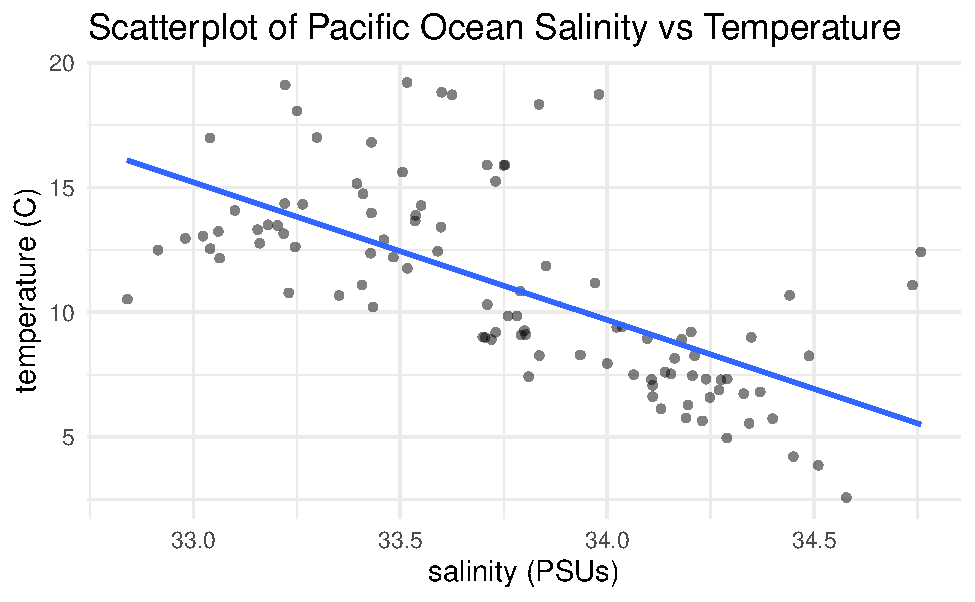
\includegraphics[width=0.7\linewidth]{13-LN013-regression_files/figure-latex/unnamed-chunk-10-1} \end{center}

\newpage

Diagnostic plots:

\begin{center}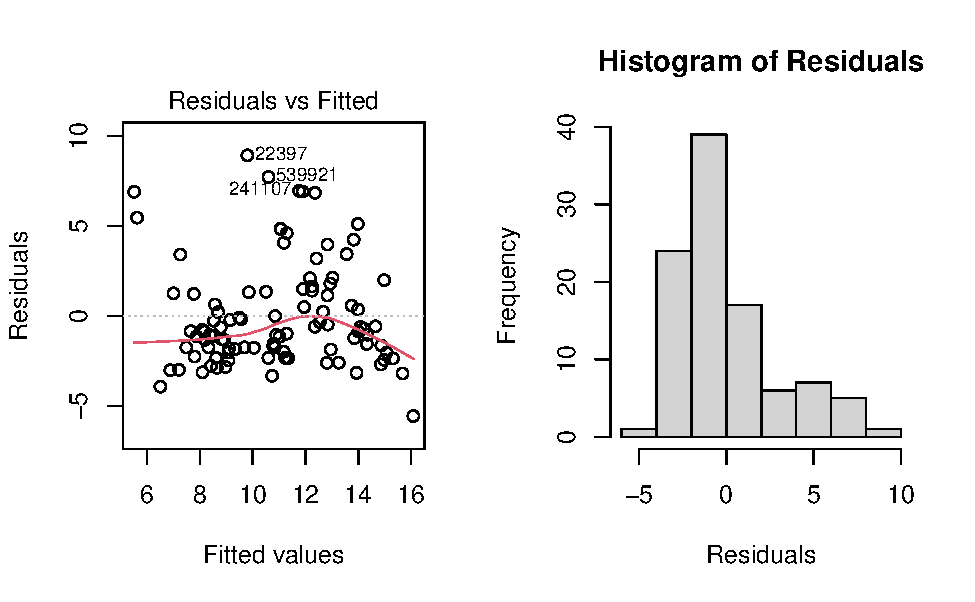
\includegraphics[width=0.7\linewidth]{13-LN013-regression_files/figure-latex/unnamed-chunk-11-1} \end{center}

Like with paired data the t-distribution can be used to model slope and correlation.

\setstretch{1.5}

\begin{itemize}
\tightlist
\item
  For two quantitative variables we use the \_\_\_\_\_\_-distribution
  with \_\_\_\_\_\_\_\_\_\_\_\_\_\_\_\_\_\_\_\_\_ degrees of freedom to approximate the sampling distribution.
\end{itemize}

\setstretch{1}

Theory-based test:

\begin{itemize}
\item
  Calculate the standardized statistic
\item
  Find the area under the t-distribution with \(n - 2\) df at least as extreme as the standardized statistic
\end{itemize}

Equation for the standardized slope:

\vspace{0.8in}

Calculate the standardized slope for the ocean data

\vspace{1in}

\begin{center}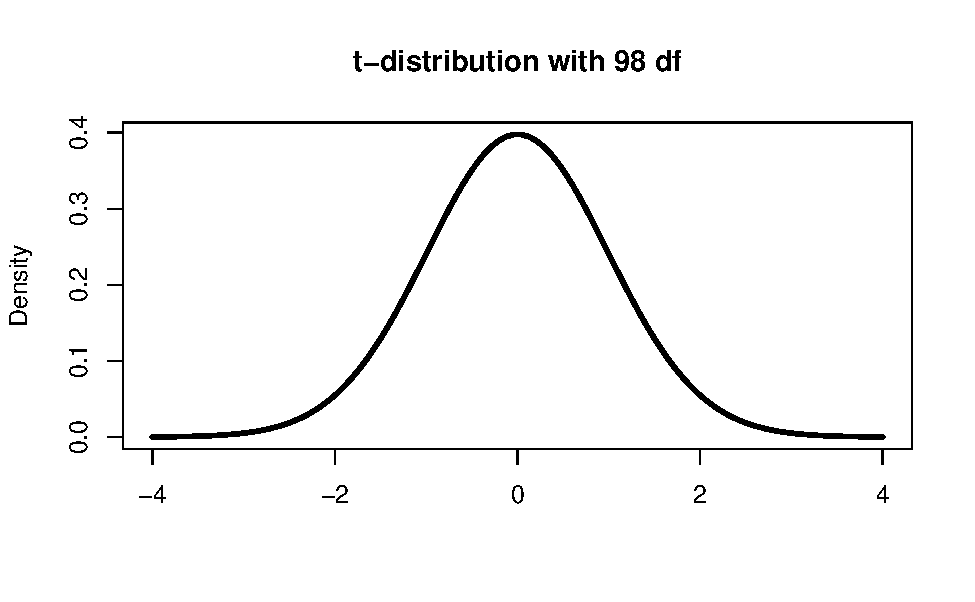
\includegraphics[width=0.7\linewidth]{13-LN013-regression_files/figure-latex/pvalueoce-1} \end{center}

Interpret the standardized statistic:

\vspace{0.8in}

To find the theory-based p-value:

\begin{Shaded}
\begin{Highlighting}[]
\NormalTok{lm.water }\OtherTok{\textless{}{-}} \FunctionTok{lm}\NormalTok{(T\_degC}\SpecialCharTok{\textasciitilde{}}\NormalTok{Salnty, }\AttributeTok{data=}\NormalTok{water) }\CommentTok{\# lm(response\textasciitilde{}explanatory)}
\FunctionTok{summary}\NormalTok{(lm.water)}\SpecialCharTok{$}\NormalTok{coefficients}
\CommentTok{\#\textgreater{}               Estimate Std. Error   t value     Pr(\textgreater{}|t|)}
\CommentTok{\#\textgreater{} (Intercept) 197.156160 21.4778118  9.179527 7.304666e{-}15}
\CommentTok{\#\textgreater{} Salnty       {-}5.513691  0.6359673 {-}8.669770 9.257446e{-}14}
\end{Highlighting}
\end{Shaded}

or

\begin{Shaded}
\begin{Highlighting}[]
\FunctionTok{pt}\NormalTok{(}\SpecialCharTok{{-}}\FloatTok{8.670}\NormalTok{, }\AttributeTok{df =} \DecValTok{98}\NormalTok{, }\AttributeTok{lower.tail=}\ConstantTok{TRUE}\NormalTok{)}
\CommentTok{\#\textgreater{} [1] 4.623445e{-}14}
\end{Highlighting}
\end{Shaded}

\hypertarget{confidence-interval-7}{%
\subsection*{Confidence interval}\label{confidence-interval-7}}
\addcontentsline{toc}{subsection}{Confidence interval}

To estimate the true slope (or true correlation) we will create a confidence interval.

\hypertarget{simulation-based-method-8}{%
\subsubsection*{Simulation-based method}\label{simulation-based-method-8}}
\addcontentsline{toc}{subsubsection}{Simulation-based method}

\begin{itemize}
\item
  Write the explanatory and response value pairs on cards
\item
  Sample pairs with replacement \(n\) times
\item
  Plot the resampled data points to find the least squares line of regression
\item
  Calculate and plot the simulated slope (or correlation) from each simulation
\item
  Repeat 1000 times (simulations) to create the bootstrap distribution
\item
  Find the cut-offs for the middle X\% (confidence level) in a bootstrap distribution.
\end{itemize}

Returning to the ocean example, we will estimate the true slope between salinity and temperature of the Pacific Ocean.

\begin{Shaded}
\begin{Highlighting}[]
\FunctionTok{set.seed}\NormalTok{(}\DecValTok{216}\NormalTok{)}
\FunctionTok{regression\_bootstrap\_CI}\NormalTok{(T\_degC}\SpecialCharTok{\textasciitilde{}}\NormalTok{Salnty, }\CommentTok{\# response \textasciitilde{} explanatory}
   \AttributeTok{data =}\NormalTok{ water, }\CommentTok{\# Name of data set}
   \AttributeTok{confidence\_level =} \FloatTok{0.95}\NormalTok{, }\CommentTok{\# Confidence level as decimal}
   \AttributeTok{summary\_measure =} \StringTok{"slope"}\NormalTok{, }\CommentTok{\# Slope or correlation}
   \AttributeTok{number\_repetitions =} \DecValTok{1000}\NormalTok{) }\CommentTok{\# Number of simulated samples for bootstrap distribution}
\end{Highlighting}
\end{Shaded}

\begin{center}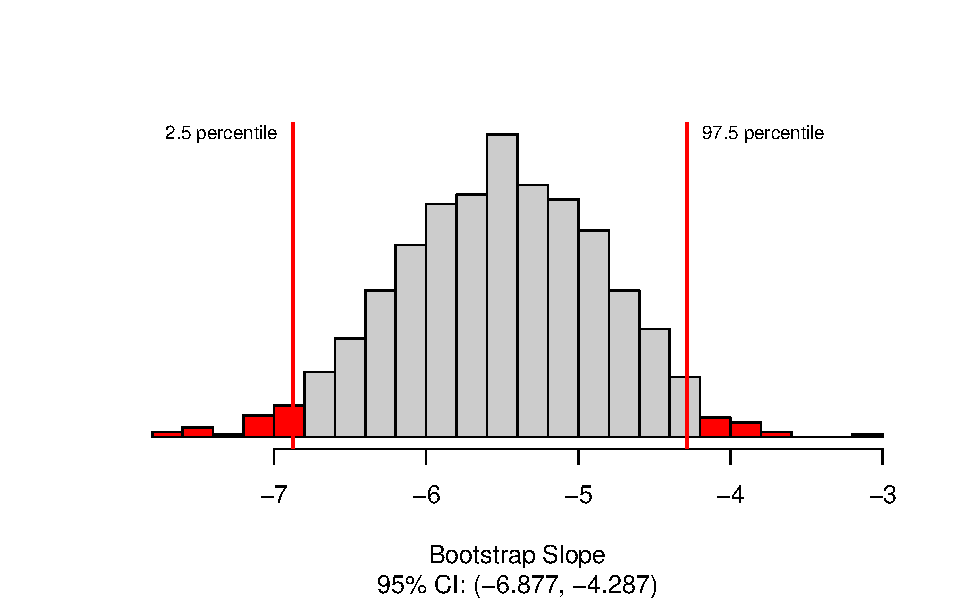
\includegraphics[width=0.7\linewidth]{13-LN013-regression_files/figure-latex/unnamed-chunk-14-1} \end{center}

Confidence interval interpretation:

\begin{itemize}
\item
  How confident you are (e.g., 90\%, 95\%, 98\%, 99\%)
\item
  Parameter of interest
\item
  Calculated interval
\item
  Order of subtraction when comparing two groups
\end{itemize}

\vspace{0.8in}

Now we will estimate the true correlation between salinity and temperature of the Pacific Ocean.

\begin{Shaded}
\begin{Highlighting}[]
\FunctionTok{set.seed}\NormalTok{(}\DecValTok{216}\NormalTok{)}
\FunctionTok{regression\_bootstrap\_CI}\NormalTok{(T\_degC}\SpecialCharTok{\textasciitilde{}}\NormalTok{Salnty, }\CommentTok{\# response \textasciitilde{} explanatory}
   \AttributeTok{data =}\NormalTok{ water, }\CommentTok{\# Name of data set}
   \AttributeTok{confidence\_level =} \FloatTok{0.95}\NormalTok{, }\CommentTok{\# Confidence level as decimal}
   \AttributeTok{summary\_measure =} \StringTok{"correlation"}\NormalTok{, }\CommentTok{\# Slope or correlation}
   \AttributeTok{number\_repetitions =} \DecValTok{1000}\NormalTok{) }\CommentTok{\# Number of simulated samples for bootstrap distribution}
\end{Highlighting}
\end{Shaded}

\begin{center}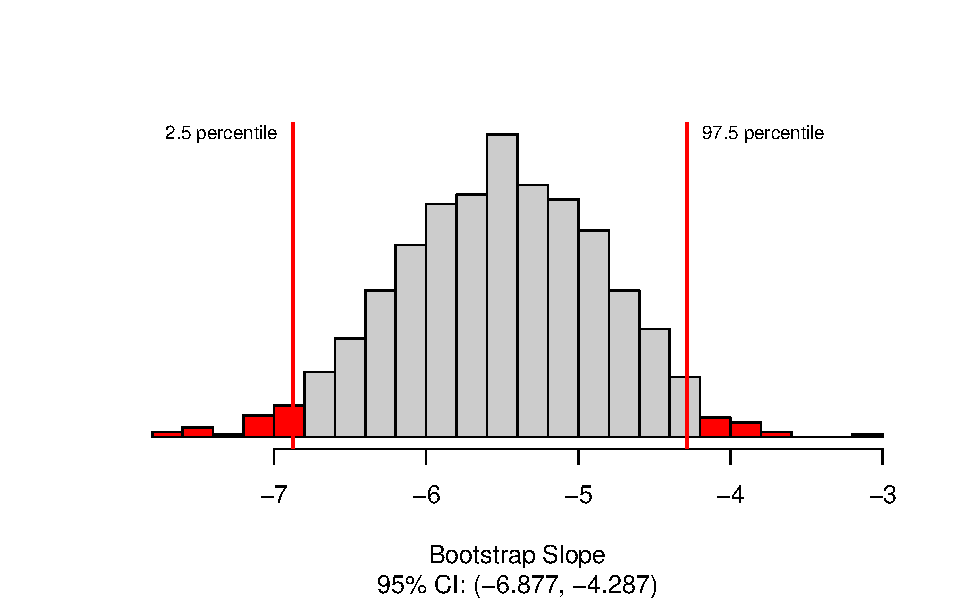
\includegraphics[width=0.7\linewidth]{13-LN013-regression_files/figure-latex/unnamed-chunk-15-1} \end{center}

Confidence interval interpretation:

\begin{itemize}
\item
  How confident you are (e.g., 90\%, 95\%, 98\%, 99\%)
\item
  Parameter of interest
\item
  Calculated interval
\item
  Order of subtraction when comparing two groups
\end{itemize}

\vspace{0.8in}

\hypertarget{theory-based-method-7}{%
\subsubsection*{Theory-based method}\label{theory-based-method-7}}
\addcontentsline{toc}{subsubsection}{Theory-based method}

\begin{itemize}
\tightlist
\item
  Calculate the interval centered at the sample statistic
\end{itemize}

\rgi \(\text{statistic} \pm \text{margin of error}\)

\vspace{0.8in}

\begin{Shaded}
\begin{Highlighting}[]
\NormalTok{lm.water }\OtherTok{\textless{}{-}} \FunctionTok{lm}\NormalTok{(T\_degC}\SpecialCharTok{\textasciitilde{}}\NormalTok{Salnty, }\AttributeTok{data=}\NormalTok{water) }\CommentTok{\# lm(response\textasciitilde{}explanatory)}
\FunctionTok{round}\NormalTok{(}\FunctionTok{summary}\NormalTok{(lm.water)}\SpecialCharTok{$}\NormalTok{coefficients, }\DecValTok{3}\NormalTok{)}
\CommentTok{\#\textgreater{}             Estimate Std. Error t value Pr(\textgreater{}|t|)}
\CommentTok{\#\textgreater{} (Intercept)  197.156     21.478    9.18        0}
\CommentTok{\#\textgreater{} Salnty        {-}5.514      0.636   {-}8.67        0}
\end{Highlighting}
\end{Shaded}

Using the ocean data, calculate the confidence interval for the true slope.

\vspace{1in}

\newpage

\hypertarget{out-of-class-activity-week-13-prediction-of-crocodylian-body-size}{%
\section{Out of Class Activity Week 13: Prediction of Crocodylian Body Size}\label{out-of-class-activity-week-13-prediction-of-crocodylian-body-size}}

\setstretch{1}

\hypertarget{learning-outcomes-8}{%
\subsection{Learning outcomes}\label{learning-outcomes-8}}

\begin{itemize}
\item
  Given a research question involving two quantitative variables, construct the null and alternative hypotheses
  in words and using appropriate statistical symbols.
\item
  Describe and perform a simulation-based hypothesis test for slope or correlation.
\item
  Interpret and evaluate a p-value for a simulation-based hypothesis test for a slope or correlation.
\item
  Use bootstrapping to find a confidence interval for the slope or correlation.
\item
  Interpret a confidence interval for a slope or correlation.
\end{itemize}

\hypertarget{terminology-review-6}{%
\subsection{Terminology review}\label{terminology-review-6}}

In today's activity, we will use simulation-based methods for hypothesis tests and confidence intervals for a linear regression slope or correlation. Some terms covered in this activity are:

\begin{itemize}
\item
  Correlation
\item
  Slope
\item
  Regression line
\end{itemize}

To review these concepts, see Chapter 21 in the textbook.

\hypertarget{crocodylian-body-size}{%
\subsection{Crocodylian Body Size}\label{crocodylian-body-size}}

Much research surrounds using measurements of animals to estimate body-size of extinct animals. Many challenges exist in making accurate estimates for extinct crocodylians. The term crocodylians refers to all members of the family Crocodylidae (``true'' crocodiles), family Alligatoridae (alligators and caimans) and family Gavialidae (gharial, Tomistoma). The researchers in this study (\textbf{obrien2019?}) state, ``Among extinct crocodylians and their precursors (e.g., suchians), several methods have been developed to predict body size from suites of hard-tissue proxies. Nevertheless, many have limited applications due to the disparity of some major suchian groups and biases in the fossil record. Here, we test the utility of head width (HW) as a broadly applicable body-size estimator in living and fossil suchians.'' Is there evidence that head width is a good predictor of body size for crocodylians?

\begin{Shaded}
\begin{Highlighting}[]
\CommentTok{\# Read in data set}
\NormalTok{croc }\OtherTok{\textless{}{-}} \FunctionTok{read.csv}\NormalTok{(}\StringTok{"https://math.montana.edu/courses/s216/data/Crocodylian\_headwidth.csv"}\NormalTok{)}
\NormalTok{croc }\OtherTok{\textless{}{-}}\NormalTok{ croc }\SpecialCharTok{\%\textgreater{}\%}
    \FunctionTok{na.omit}\NormalTok{()}
\end{Highlighting}
\end{Shaded}

\hypertarget{vocabulary-review}{%
\subsubsection*{Vocabulary review}\label{vocabulary-review}}
\addcontentsline{toc}{subsubsection}{Vocabulary review}

\begin{enumerate}
\def\labelenumi{\arabic{enumi}.}
\tightlist
\item
  Explain why regression methods are appropriate to use to address the researchers' question. Make sure you clearly define the variables of interest in your explanation and their roles.
\end{enumerate}

\vspace{.5in}

To create a scatterplot to examine the relationship between head width and total body length we will use \texttt{HW\_cm} as the explanatory variable and \texttt{TL\_cm} as the response variable.

\begin{Shaded}
\begin{Highlighting}[]
\NormalTok{croc }\SpecialCharTok{\%\textgreater{}\%} \CommentTok{\# Pipe data set into...}
\FunctionTok{ggplot}\NormalTok{(}\FunctionTok{aes}\NormalTok{(}\AttributeTok{x =}\NormalTok{ HW\_cm, }\AttributeTok{y =}\NormalTok{ TL\_cm))}\SpecialCharTok{+}  \CommentTok{\# Specify variables}
  \FunctionTok{geom\_point}\NormalTok{() }\SpecialCharTok{+}  \CommentTok{\# Add scatterplot of points}
  \FunctionTok{labs}\NormalTok{(}\AttributeTok{x =} \StringTok{"head width (cm)"}\NormalTok{,  }\CommentTok{\# Label x{-}axis}
       \AttributeTok{y =} \StringTok{"total length (cm)"}\NormalTok{,  }\CommentTok{\# Label y{-}axis}
       \AttributeTok{title =} \StringTok{"Scatterplot of Crocodylian Head Width vs. Total Length"}\NormalTok{) }\SpecialCharTok{+} 
               \CommentTok{\# Be sure to title your plots}
  \FunctionTok{geom\_smooth}\NormalTok{(}\AttributeTok{method =} \StringTok{"lm"}\NormalTok{, }\AttributeTok{se =} \ConstantTok{FALSE}\NormalTok{)  }\CommentTok{\# Add regression line}
\end{Highlighting}
\end{Shaded}

\begin{center}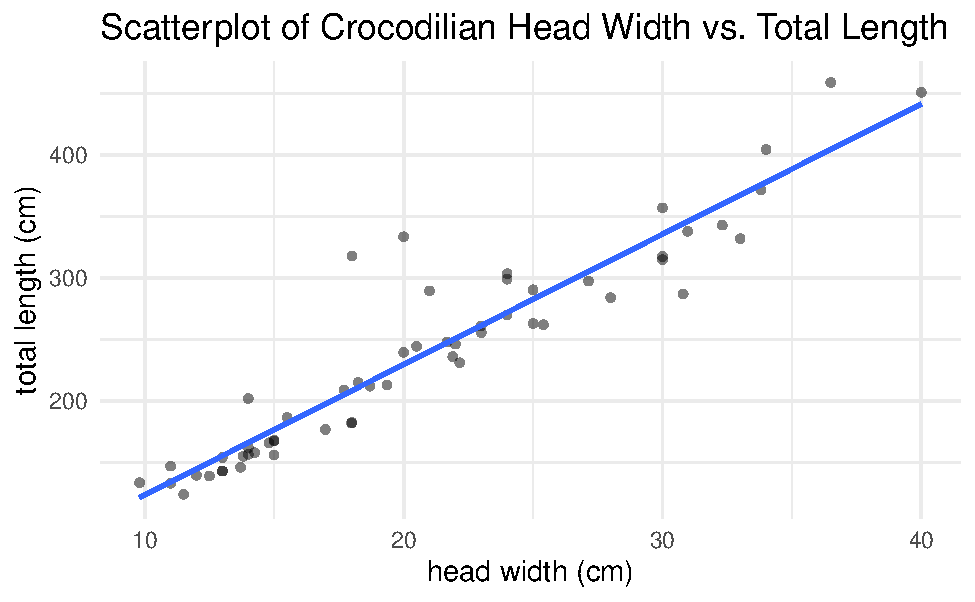
\includegraphics[width=0.7\linewidth]{13-OCA10-regression-simulation_files/figure-latex/unnamed-chunk-2-1} \end{center}

\begin{enumerate}
\def\labelenumi{\arabic{enumi}.}
\setcounter{enumi}{1}
\tightlist
\item
  Describe the features of the plot above, addressing all four characteristics of a scatterplot.
\end{enumerate}

\vspace{1in}

~~~~~~~If you indicated there are potential outliers, which points are they?

\vspace{0.5in}

\hypertarget{ask-a-research-question-4}{%
\subsubsection*{Ask a research question}\label{ask-a-research-question-4}}
\addcontentsline{toc}{subsubsection}{Ask a research question}

\begin{enumerate}
\def\labelenumi{\arabic{enumi}.}
\setcounter{enumi}{2}
\tightlist
\item
  Write out the null hypothesis in words to test \textbf{slope}.
\end{enumerate}

\vspace{0.8in}

\begin{enumerate}
\def\labelenumi{\arabic{enumi}.}
\setcounter{enumi}{3}
\tightlist
\item
  Using the research question, write the alternative hypothesis in notation using \textbf{slope} as the summary measure.
\end{enumerate}

\vspace{0.5in}

\hypertarget{summarize-and-visualize-the-data-4}{%
\subsubsection*{Summarize and visualize the data}\label{summarize-and-visualize-the-data-4}}
\addcontentsline{toc}{subsubsection}{Summarize and visualize the data}

The linear model output for the data is given below.

\begin{Shaded}
\begin{Highlighting}[]
\NormalTok{lm.croc }\OtherTok{\textless{}{-}} \FunctionTok{lm}\NormalTok{(TL\_cm}\SpecialCharTok{\textasciitilde{}}\NormalTok{HW\_cm, }\AttributeTok{data=}\NormalTok{croc) }\CommentTok{\# lm(response\textasciitilde{}explanatory)}
\FunctionTok{round}\NormalTok{(}\FunctionTok{summary}\NormalTok{(lm.croc)}\SpecialCharTok{$}\NormalTok{coefficients, }\DecValTok{5}\NormalTok{)}
\CommentTok{\#\textgreater{}             Estimate Std. Error  t value Pr(\textgreater{}|t|)}
\CommentTok{\#\textgreater{} (Intercept) 17.61250   11.36269  1.55003  0.12687}
\CommentTok{\#\textgreater{} HW\_cm       10.59983    0.51294 20.66494  0.00000}
\end{Highlighting}
\end{Shaded}

The value of correlation is given below.

\begin{Shaded}
\begin{Highlighting}[]
\FunctionTok{cor}\NormalTok{(croc}\SpecialCharTok{$}\NormalTok{HW\_cm, croc}\SpecialCharTok{$}\NormalTok{TL\_cm)}
\CommentTok{\#\textgreater{} [1] 0.9412234}
\end{Highlighting}
\end{Shaded}

\begin{enumerate}
\def\labelenumi{\arabic{enumi}.}
\setcounter{enumi}{4}
\item
  Using the output from the evaluated R code above, write the equation of the regression line in the context of the problem using appropriate statistical notation.
  \vspace{1in}
\item
  Interpret the estimated slope in context of the problem.
\end{enumerate}

\vspace{1in}

\begin{enumerate}
\def\labelenumi{\arabic{enumi}.}
\setcounter{enumi}{6}
\tightlist
\item
  Report the value of correlation between head width and total body length.
\end{enumerate}

\vspace{0.3in}

\hypertarget{use-statistical-inferential-methods-to-draw-inferences-from-the-data-5}{%
\subsubsection*{Use statistical inferential methods to draw inferences from the data}\label{use-statistical-inferential-methods-to-draw-inferences-from-the-data-5}}
\addcontentsline{toc}{subsubsection}{Use statistical inferential methods to draw inferences from the data}

In this activity, we will focus on using simulation-based methods for inference in regression.

\hypertarget{simulation-based-hypothesis-test}{%
\subsubsection*{Simulation-based hypothesis test}\label{simulation-based-hypothesis-test}}
\addcontentsline{toc}{subsubsection}{Simulation-based hypothesis test}

Let's start by thinking about how one simulation would be created on the null distribution using cards. First, we would write the values for the response variable, total length, on each card. Next, we would shuffle these \(y\) values while keeping the \(x\) values (explanatory variable) in the same order. Then, find the line of regression for the shuffled \((x, y)\) pairs and calculate either the slope or correlation of the shuffled sample.

We will use the \texttt{regression\_test()} function in R (in the \texttt{catstats} package) to simulate the null distribution of shuffled slopes (or shuffled correlations) and compute a p-value. We will need to enter the response variable name and the explanatory variable name for the formula, the data set name (identified above as \texttt{croc}), the summary measure for the test (either slope or correlation), number of repetitions, the sample statistic (value of slope or correlation), and the direction of the alternative hypothesis.

The response variable name is \texttt{TL\_cm} and the explanatory variable name is \texttt{HW\_cm} for these data.

\begin{enumerate}
\def\labelenumi{\arabic{enumi}.}
\setcounter{enumi}{7}
\tightlist
\item
  What inputs should be entered for each of the following to create the simulation to test regression slope?
\end{enumerate}

\vspace{.5 mm}

\begin{itemize}
\tightlist
\item
  Direction (\texttt{"greater"}, \texttt{"less"}, or \texttt{"two-sided"}):
\end{itemize}

\vspace{.2in}

\begin{itemize}
\tightlist
\item
  Summary measure (choose \texttt{"slope"} or \texttt{"correlation"}):
\end{itemize}

\vspace{.2in}

\begin{itemize}
\tightlist
\item
  As extreme as (enter the value for the sample slope):
\end{itemize}

\vspace{0.2in}

\begin{itemize}
\tightlist
\item
  Number of repetitions:
\end{itemize}

\vspace{.2in}

Check that your answers to question 8 reflect what is shown below in the R code to produce the null distribution for slope.

\begin{Shaded}
\begin{Highlighting}[]
\FunctionTok{set.seed}\NormalTok{(}\DecValTok{216}\NormalTok{)}
\FunctionTok{regression\_test}\NormalTok{(TL\_cm}\SpecialCharTok{\textasciitilde{}}\NormalTok{HW\_cm, }\CommentTok{\# response \textasciitilde{} explanatory}
               \AttributeTok{data =}\NormalTok{ croc, }\CommentTok{\# Name of data set}
               \AttributeTok{direction =} \StringTok{"two{-}sided"}\NormalTok{, }\CommentTok{\# Sign in alternative ("greater", "less", "two{-}sided")}
               \AttributeTok{summary\_measure =} \StringTok{"slope"}\NormalTok{, }\CommentTok{\# "slope" or "correlation"}
               \AttributeTok{as\_extreme\_as =} \FloatTok{10.600}\NormalTok{, }\CommentTok{\# Observed slope or correlation}
               \AttributeTok{number\_repetitions =} \DecValTok{1000}\NormalTok{) }\CommentTok{\# Number of simulated samples for null distribution}
\end{Highlighting}
\end{Shaded}

\begin{center}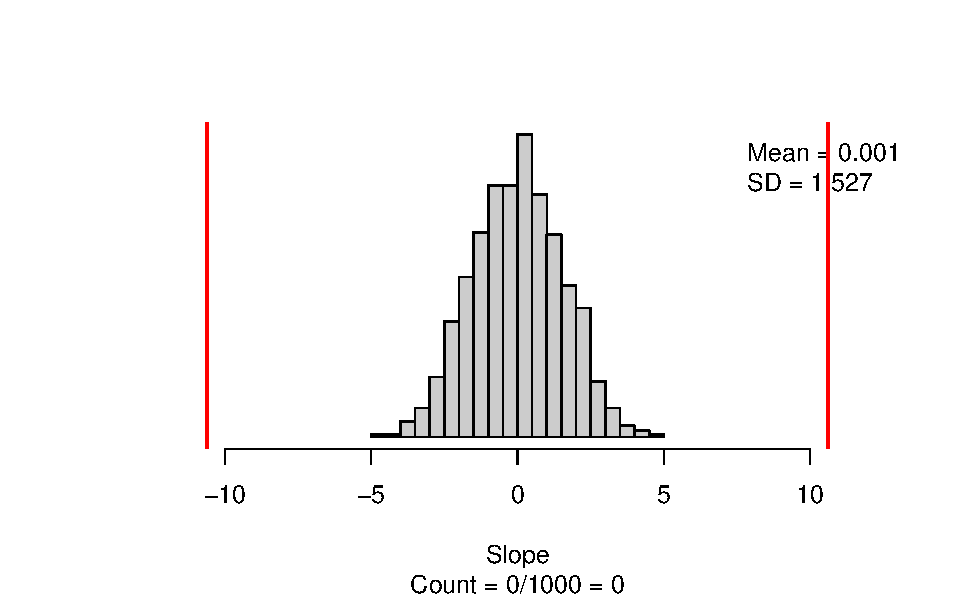
\includegraphics[width=0.7\linewidth]{13-OCA10-regression-simulation_files/figure-latex/unnamed-chunk-5-1} \end{center}

\begin{enumerate}
\def\labelenumi{\arabic{enumi}.}
\setcounter{enumi}{8}
\item
  Report the p-value from the R output.
  \vspace{0.5in}
\item
  Suppose we wanted to complete the simulation test using correlation as the summary measure, instead of slope. Which two inputs in \#8 would need to be changed to test for correlation? What inputs should you use instead?
  \vspace{0.75in}
\end{enumerate}

Check that your answers to question 10 reflect what is shown below in the R code to produce the null distribution for correlation.

\begin{Shaded}
\begin{Highlighting}[]
\FunctionTok{set.seed}\NormalTok{(}\DecValTok{216}\NormalTok{)}
\FunctionTok{regression\_test}\NormalTok{(TL\_cm}\SpecialCharTok{\textasciitilde{}}\NormalTok{HW\_cm, }\CommentTok{\# response \textasciitilde{} explanatory}
               \AttributeTok{data =}\NormalTok{ croc, }\CommentTok{\# Name of data set}
               \AttributeTok{direction =} \StringTok{"two{-}sided"}\NormalTok{, }\CommentTok{\# Sign in alternative ("greater", "less", "two{-}sided")}
               \AttributeTok{summary\_measure =} \StringTok{"correlation"}\NormalTok{, }\CommentTok{\# "slope" or "correlation"}
               \AttributeTok{as\_extreme\_as =} \FloatTok{0.941}\NormalTok{, }\CommentTok{\# Observed slope or correlation}
               \AttributeTok{number\_repetitions =} \DecValTok{1000}\NormalTok{) }\CommentTok{\# Number of simulated samples for null distribution}
\end{Highlighting}
\end{Shaded}

\begin{center}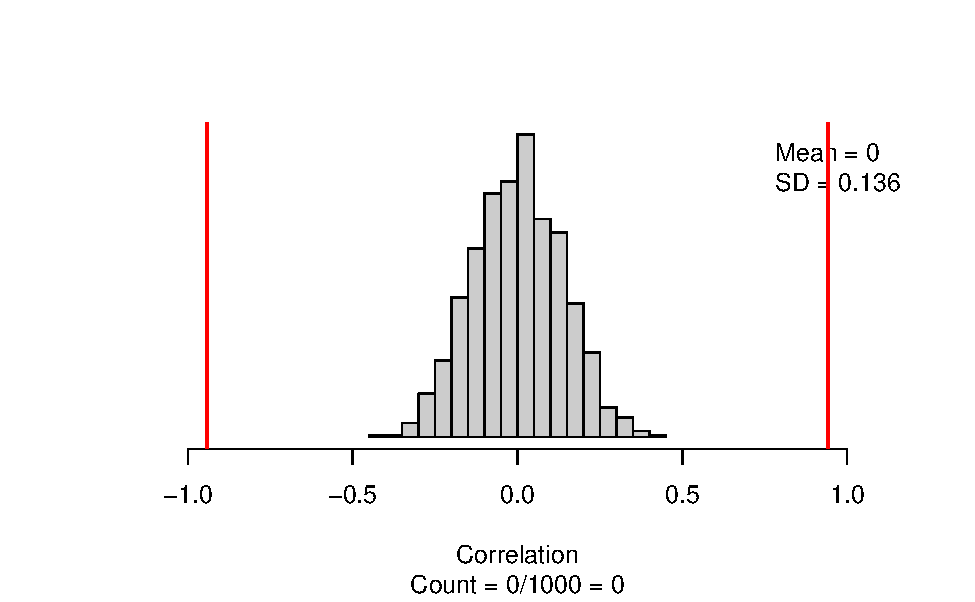
\includegraphics[width=0.7\linewidth]{13-OCA10-regression-simulation_files/figure-latex/unnamed-chunk-6-1} \end{center}

\begin{enumerate}
\def\labelenumi{\arabic{enumi}.}
\setcounter{enumi}{10}
\tightlist
\item
  The p-values from the test of slope and the test of correlation should be similar. Explain why the two p-values should match. \emph{Hint: think about the relationship between slope and correlation!}
  \vspace{1in}
\end{enumerate}

\hypertarget{simulation-based-confidence-interval}{%
\subsubsection*{Simulation-based confidence interval}\label{simulation-based-confidence-interval}}
\addcontentsline{toc}{subsubsection}{Simulation-based confidence interval}

We will use the \texttt{regression\_bootstrap\_CI()} function in R (in the \texttt{catstats} package) to simulate the bootstrap distribution of sample slopes (or sample correlations) and calculate a confidence interval. The following code gives the 95\% confidence interval for the true slope.

\begin{Shaded}
\begin{Highlighting}[]
\FunctionTok{set.seed}\NormalTok{(}\DecValTok{216}\NormalTok{)}
\FunctionTok{regression\_bootstrap\_CI}\NormalTok{(TL\_cm}\SpecialCharTok{\textasciitilde{}}\NormalTok{HW\_cm, }\CommentTok{\# response \textasciitilde{} explanatory}
   \AttributeTok{data =}\NormalTok{ croc, }\CommentTok{\# Name of data set}
   \AttributeTok{confidence\_level =} \FloatTok{0.95}\NormalTok{, }\CommentTok{\# Confidence level as decimal}
   \AttributeTok{summary\_measure =} \StringTok{"slope"}\NormalTok{, }\CommentTok{\# Slope or correlation}
   \AttributeTok{number\_repetitions =} \DecValTok{1000}\NormalTok{) }\CommentTok{\# Number of simulated samples for bootstrap distribution}
\end{Highlighting}
\end{Shaded}

\begin{center}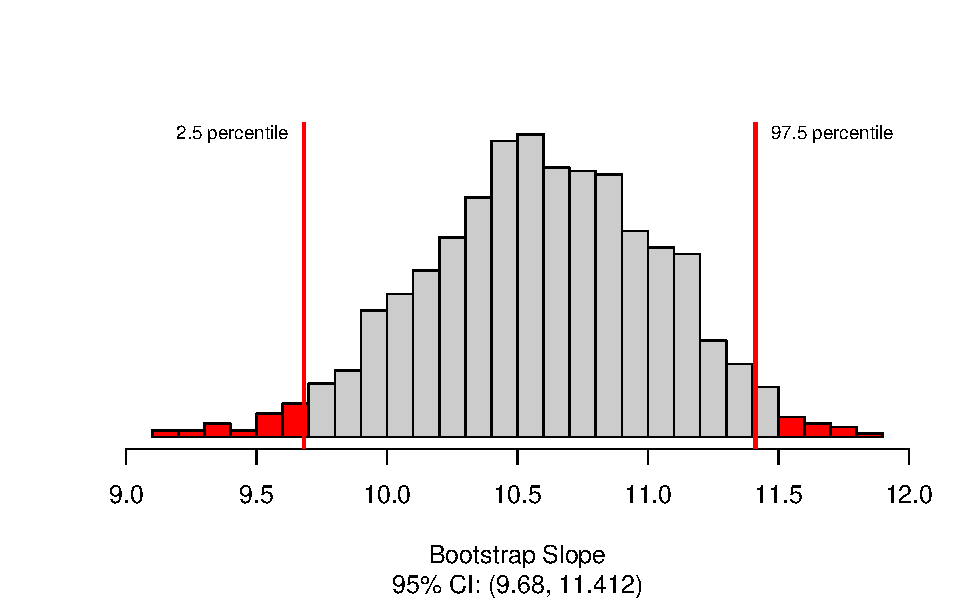
\includegraphics[width=0.7\linewidth]{13-OCA10-regression-simulation_files/figure-latex/unnamed-chunk-7-1} \end{center}

\begin{enumerate}
\def\labelenumi{\arabic{enumi}.}
\setcounter{enumi}{11}
\item
  Report the bootstrap 95\% confidence interval in interval notation.\\
  \vspace{0.5in}
\item
  Interpret the interval in question 12 in context of the problem. \emph{Hint: use the interpretation of slope in your confidence interval interpretation.}
\end{enumerate}

\vspace{0.8in}

\hypertarget{communicate-the-results-and-answer-the-research-question-4}{%
\subsubsection*{Communicate the results and answer the research question}\label{communicate-the-results-and-answer-the-research-question-4}}
\addcontentsline{toc}{subsubsection}{Communicate the results and answer the research question}

\begin{enumerate}
\def\labelenumi{\arabic{enumi}.}
\setcounter{enumi}{13}
\tightlist
\item
  Based on the p-value, write a conclusion in context of the problem.
\end{enumerate}

\vspace{.8in}

\begin{enumerate}
\def\labelenumi{\arabic{enumi}.}
\setcounter{enumi}{14}
\tightlist
\item
  Does the conclusion based on the p-value agree with the results of the 95\% confidence interval? What does each tell you about the null hypothesis?
\end{enumerate}

\vspace{.6in}
\newpage

\hypertarget{take-home-messages-6}{%
\subsection{Take-home messages}\label{take-home-messages-6}}

\begin{enumerate}
\def\labelenumi{\arabic{enumi}.}
\item
  The p-value for a test for correlation should be approximately the same as the p-value for the test of slope. In the simulation test, we just change the statistic type from slope to correlation and use the appropriate sample statistic value.
\item
  To interpret a confidence interval for the slope, think about how to interpret the sample slope and use that information in the confidence interval interpretation for slope.
\item
  To create one simulated sample on the null distribution when testing for a relationship between two quantitative variables, hold the \(x\) values constant and shuffle the \(y\) values to new \(x\) values. Find the regression line for the shuffled data and plot the slope or the correlation for the shuffled data.
\item
  To create one simulated sample on the bootstrap distribution when assessing two quantitative variables, label \(n\) cards with the original (response, explanatory) values. Randomly draw with replacement \(n\) times. Find the regression line for the resampled data and plot the resampled slope or correlation.
\end{enumerate}

\hypertarget{additional-notes-6}{%
\subsection{Additional notes}\label{additional-notes-6}}

Use this space to summarize your thoughts and take additional notes on today's activity and material covered.

\newpage

\hypertarget{activity-13-golf-driving-distance}{%
\section{Activity 13: Golf Driving Distance}\label{activity-13-golf-driving-distance}}

\setstretch{1}

\hypertarget{learning-outcomes-9}{%
\subsection{Learning outcomes}\label{learning-outcomes-9}}

\begin{itemize}
\item
  Given a research question involving two quantitative variables, construct the null and alternative hypotheses
  in words and using appropriate statistical symbols.
\item
  Assess the conditions to use the normal distribution model for a slope.
\item
  Find the T test statistic (T-score) for a slope based off of \texttt{lm()} output in R.
\item
  Find, interpret, and evaluate the p-value for a theory-based hypothesis test for a slope.
\item
  Create and interpret a theory-based confidence interval for a slope.
\item
  Use a confidence interval to determine the conclusion of a hypothesis test.
\end{itemize}

\hypertarget{terminology-review-7}{%
\subsection{Terminology review}\label{terminology-review-7}}

In this week's in-class activity, we will use theory-based methods for hypothesis tests and confidence intervals for a linear regression slope. Some terms covered in this activity are:

\begin{itemize}
\item
  Slope
\item
  Regression line
\end{itemize}

To review these concepts, see Chapter 21 in the textbook.

\hypertarget{golf-driving-distance}{%
\subsection{Golf driving distance}\label{golf-driving-distance}}

In golf the goal is to complete a hole with as few strokes as possible. A long driving distance to start a hole can help minimize the strokes necessary to complete the hole, as long as that drive stays on the fairway. Data was collecting on 354 PGA and LPGA players in 2008 ({``Average Driving Distance and Fairway Accuracy''} 2008). For each player, the average driving distance (yards), fairway accuracy (percentage), and sex was measured. Use these data to assess, ``Does a professional golfer give up accuracy when they hit the ball farther?''

\begin{Shaded}
\begin{Highlighting}[]
\CommentTok{\# Read in data set}
\NormalTok{golf }\OtherTok{\textless{}{-}} \FunctionTok{read.csv}\NormalTok{(}\StringTok{"https://math.montana.edu/courses/s216/data/golf.csv"}\NormalTok{)}
\end{Highlighting}
\end{Shaded}

\hypertarget{plot-review.}{%
\subsubsection*{Plot review.}\label{plot-review.}}
\addcontentsline{toc}{subsubsection}{Plot review.}

Use the provided R script file to create a scatterplot to examine the relationship between the driving distance and percent accuracy by filling in the variable names (\texttt{Driving\_Distance} and \texttt{Percent\_Accuracy}) for \texttt{xx} and \texttt{yy} in line 9. Highlight and run lines 1--15.

\begin{Shaded}
\begin{Highlighting}[]
\NormalTok{golf }\SpecialCharTok{\%\textgreater{}\%} \CommentTok{\# Pipe data set into...}
\FunctionTok{ggplot}\NormalTok{(}\FunctionTok{aes}\NormalTok{(}\AttributeTok{x =}\NormalTok{ xx, }\AttributeTok{y =}\NormalTok{ yy))}\SpecialCharTok{+}  \CommentTok{\# Specify variables}
  \FunctionTok{geom\_point}\NormalTok{() }\SpecialCharTok{+}  \CommentTok{\# Add scatterplot of points}
  \FunctionTok{labs}\NormalTok{(}\AttributeTok{x =} \StringTok{"Driving Distance"}\NormalTok{,  }\CommentTok{\# Label x{-}axis}
       \AttributeTok{y =} \StringTok{"Percent Accuracy"}\NormalTok{,  }\CommentTok{\# Label y{-}axis}
       \AttributeTok{title =} \StringTok{"Scatterplot of Driving Distance by Percent Accuracy"}\NormalTok{) }\SpecialCharTok{+} 
               \CommentTok{\# Be sure to tile your plots}
  \FunctionTok{geom\_smooth}\NormalTok{(}\AttributeTok{method =} \StringTok{"lm"}\NormalTok{, }\AttributeTok{se =} \ConstantTok{FALSE}\NormalTok{)  }\CommentTok{\# Add regression line}
\end{Highlighting}
\end{Shaded}

\begin{enumerate}
\def\labelenumi{\arabic{enumi}.}
\tightlist
\item
  Sketch the plot created below. Based on your plot, does it appear that there is a relationship between driving distance and percent accuracy? Note: \texttt{Driving\ Distance} should be on the \(x\)-axis.
\end{enumerate}

\vspace{2in}

\hypertarget{conditions-for-the-least-squares-line}{%
\subsubsection*{Conditions for the least squares line}\label{conditions-for-the-least-squares-line}}
\addcontentsline{toc}{subsubsection}{Conditions for the least squares line}

When performing inference on a least squares line, the follow conditions are generally required:

\begin{itemize}
\tightlist
\item
  \emph{Independent observations} (for both simulation-based and theory-based methods): individual data points must be independent.

  \begin{itemize}
  \tightlist
  \item
    Check this assumption by investigating the sampling method and determining if the observational units are related in any way.
  \end{itemize}
\item
  \emph{Linearity} (for both simulation-based and theory-based methods): the data should follow a linear trend.

  \begin{itemize}
  \tightlist
  \item
    Check this assumption by examining the scatterplot of the two variables, and a scatterplot of the residuals (on the \(y\)-axis) versus the fitted values (on the \(x\)-axis). The pattern in the residual plot should display a horizontal line.
  \end{itemize}
\item
  \emph{Constant variability} (for theory-based methods only): the variability of points around the least squares line remains roughly constant

  \begin{itemize}
  \tightlist
  \item
    Check this assumption by examining a scatterplot of the residuals (on the \(y\)-axis) versus the fitted values (on the \(x\)-axis). The variability in the residuals around zero should be approximately the same for all fitted values.
  \end{itemize}
\item
  \emph{Nearly normal residuals} (for theory-based methods only: residuals must be nearly normal.

  \begin{itemize}
  \tightlist
  \item
    Check this assumption by examining a histogram of the residuals, which should appear approximately normal\footnote{A better plot for checking the normality assumption is called a \emph{normal quantile-quantile plot} (or QQ-plot). However, this type of plot will be covered in a future course}.
  \end{itemize}
\end{itemize}

\newpage

The scatterplot generated in question 1 and the residual plots shown below will be used to assess these conditions for approximating the data with the \(t\)-distribution.

\begin{center}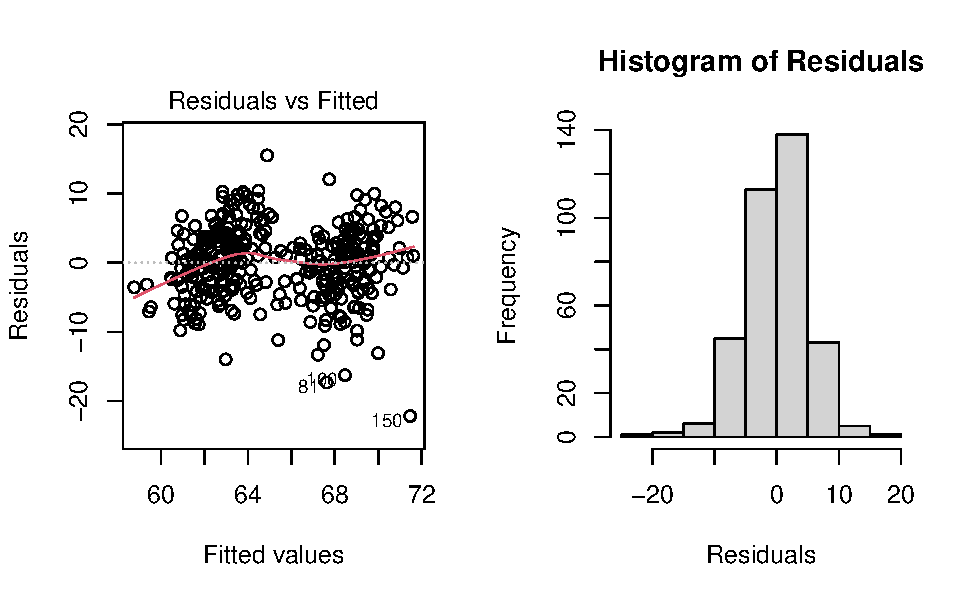
\includegraphics[width=0.7\linewidth]{13-A11-regression-theory_files/figure-latex/unnamed-chunk-3-1} \end{center}

\begin{enumerate}
\def\labelenumi{\arabic{enumi}.}
\setcounter{enumi}{1}
\tightlist
\item
  Are the conditions met to use the \(t\)-distribution to approximate the sampling distribution of the standardized statistic? Justify your answer.
\end{enumerate}

\vspace{1.5in}

\hypertarget{ask-a-research-question-5}{%
\subsubsection*{Ask a research question}\label{ask-a-research-question-5}}
\addcontentsline{toc}{subsubsection}{Ask a research question}

\begin{enumerate}
\def\labelenumi{\arabic{enumi}.}
\setcounter{enumi}{2}
\tightlist
\item
  Write out the null hypothesis in words to test the slope.
\end{enumerate}

\vspace{1in}

\begin{enumerate}
\def\labelenumi{\arabic{enumi}.}
\setcounter{enumi}{3}
\tightlist
\item
  Using the research question, write the alternative hypothesis in notation to test the slope.
\end{enumerate}

\newpage

\hypertarget{summarize-and-visualize-the-data-5}{%
\subsubsection*{Summarize and visualize the data}\label{summarize-and-visualize-the-data-5}}
\addcontentsline{toc}{subsubsection}{Summarize and visualize the data}

Using the provided R script file, enter the response variable name, \texttt{Percent\_Accuracy}, into the \texttt{lm()} (linear model) function for \texttt{response} and the explanatory variable name, \texttt{Driving\_Distance}, for \texttt{explanatory} in line 25 to get the linear model output. Highlight and run lines 25--26.

\begin{Shaded}
\begin{Highlighting}[]
\NormalTok{lm.golf }\OtherTok{\textless{}{-}} \FunctionTok{lm}\NormalTok{(response}\SpecialCharTok{\textasciitilde{}}\NormalTok{explanatory, }\AttributeTok{data=}\NormalTok{golf) }\CommentTok{\# lm(response\textasciitilde{}explanatory)}
\FunctionTok{round}\NormalTok{(}\FunctionTok{summary}\NormalTok{(lm.golf)}\SpecialCharTok{$}\NormalTok{coefficients, }\DecValTok{5}\NormalTok{)}
\end{Highlighting}
\end{Shaded}

\begin{enumerate}
\def\labelenumi{\arabic{enumi}.}
\setcounter{enumi}{4}
\tightlist
\item
  Using the output from the evaluated R code above, write the equation of the regression line in the context of the problem using appropriate statistical notation.
\end{enumerate}

\vspace{1in}

\begin{enumerate}
\def\labelenumi{\arabic{enumi}.}
\setcounter{enumi}{5}
\tightlist
\item
  Interpret the estimated slope in context of the problem.
\end{enumerate}

\vspace{1in}

\hypertarget{use-statistical-inferential-methods-to-draw-inferences-from-the-data-6}{%
\subsubsection*{Use statistical inferential methods to draw inferences from the data}\label{use-statistical-inferential-methods-to-draw-inferences-from-the-data-6}}
\addcontentsline{toc}{subsubsection}{Use statistical inferential methods to draw inferences from the data}

\hypertarget{hypothesis-test-3}{%
\paragraph*{Hypothesis test}\label{hypothesis-test-3}}
\addcontentsline{toc}{paragraph}{Hypothesis test}

To find the value of the standardized statistic to test the slope we will use,

\[
T = \frac{\mbox{slope estimate}}{SE} = \frac{b_1}{SE(b_1)}.
\]

We will use the linear model R output above to get the estimate for slope and the standard error of the slope.

\begin{enumerate}
\def\labelenumi{\arabic{enumi}.}
\setcounter{enumi}{6}
\item
  What are the values of \(b_1\) and \(SE(b_1)\)? Where in the linear model R output can you find these values?
  \vspace{0.5in}
\item
  Calculate the standardized statistic for slope. Identify where this calculated value is in the linear model R output.
\end{enumerate}

\newpage

\begin{enumerate}
\def\labelenumi{\arabic{enumi}.}
\setcounter{enumi}{8}
\tightlist
\item
  Interpret the standardized statistic in context of the problem.
\end{enumerate}

\vspace{0.8in}

\begin{enumerate}
\def\labelenumi{\arabic{enumi}.}
\setcounter{enumi}{9}
\tightlist
\item
  The p-value in the linear model R output is the two-sided p-value for the test of significance for slope. Report the p-value to answer the research question.
\end{enumerate}

\vspace{0.5in}

\begin{enumerate}
\def\labelenumi{\arabic{enumi}.}
\setcounter{enumi}{10}
\tightlist
\item
  Based on the p-value, how much evidence is there against the null hypothesis?
\end{enumerate}

\vspace{0.5in}

\hypertarget{confidence-interval-8}{%
\paragraph*{Confidence interval}\label{confidence-interval-8}}
\addcontentsline{toc}{paragraph}{Confidence interval}

Recall that a confidence interval is calculated by adding and subtracting the margin of error to the point estimate.\\
\[\mbox{point estimate}\pm t^*SE(\mbox{estimate}).\]
When the point estimate is a regression slope, this formula becomes
\[b_1 \pm t^* SE(b_1).\]

The \(t^*\) multiplier comes from a \(t\)-distribution with \(n-2\) degrees of freedom. Recall for a 95\% confidence interval, we use the 97.5\% percentile (95\% of the distribution is in the middle, leaving 2.5\% in each tail). The sample size for this study is 354 so we will use the degrees of freedom 352 (\(n-2\)).

\begin{Shaded}
\begin{Highlighting}[]
\FunctionTok{qt}\NormalTok{(}\FloatTok{0.975}\NormalTok{, }\DecValTok{352}\NormalTok{) }\CommentTok{\# 95\% t* multiplier }
\end{Highlighting}
\end{Shaded}

\begin{verbatim}
#> [1] 1.966726
\end{verbatim}

\begin{enumerate}
\def\labelenumi{\arabic{enumi}.}
\setcounter{enumi}{11}
\item
  Calculate the 95\% confidence interval for the true slope.
  \vspace{0.8in}
\item
  Interpret the 95\% confidence interval in context of the problem.
\end{enumerate}

\vspace{.8in}

\hypertarget{communicate-the-results-and-answer-the-research-question-5}{%
\subsubsection*{Communicate the results and answer the research question}\label{communicate-the-results-and-answer-the-research-question-5}}
\addcontentsline{toc}{subsubsection}{Communicate the results and answer the research question}

\begin{enumerate}
\def\labelenumi{\arabic{enumi}.}
\setcounter{enumi}{13}
\tightlist
\item
  Write a conclusion to answer the research question in context of the problem.
\end{enumerate}

\vspace{.8in}

\hypertarget{multivariate-plots}{%
\subsection*{Multivariate plots}\label{multivariate-plots}}
\addcontentsline{toc}{subsection}{Multivariate plots}

Another variable that may affect the percent accuracy is the sex of the golfer. We will look at how this variable may change the relationship between driving distance and percent accuracy. Highlight and run lines 32--39 to produce the multivariate plot.

\begin{Shaded}
\begin{Highlighting}[]
\NormalTok{golf }\SpecialCharTok{\%\textgreater{}\%}
  \FunctionTok{ggplot}\NormalTok{(}\FunctionTok{aes}\NormalTok{(}\AttributeTok{x =}\NormalTok{ Driving\_Distance, }\AttributeTok{y =}\NormalTok{ Percent\_Accuracy, }\AttributeTok{color=}\NormalTok{Sex))}\SpecialCharTok{+}  \CommentTok{\# Specify variables}
  \FunctionTok{geom\_point}\NormalTok{(}\FunctionTok{aes}\NormalTok{(}\AttributeTok{shape =}\NormalTok{ Sex), }\AttributeTok{size =} \DecValTok{3}\NormalTok{) }\SpecialCharTok{+}  \CommentTok{\# Add scatterplot of points}
  \FunctionTok{labs}\NormalTok{(}\AttributeTok{x =} \StringTok{"Driving Distance (m)"}\NormalTok{,  }\CommentTok{\# Label x{-}axis}
       \AttributeTok{y =} \StringTok{"Percent Accuracy"}\NormalTok{,  }\CommentTok{\# Label y{-}axis}
       \AttributeTok{color =} \StringTok{"Sex"}\NormalTok{, }\AttributeTok{shape =} \StringTok{"Sex"}\NormalTok{,}
       \CommentTok{\# Be sure to title your plots}
       \AttributeTok{title =} \StringTok{"Scatterplot of Golf Driving Distance and Percent Accuracy by Sex"}\NormalTok{) }\SpecialCharTok{+} 
  \FunctionTok{geom\_smooth}\NormalTok{(}\AttributeTok{method =} \StringTok{"lm"}\NormalTok{, }\AttributeTok{se =} \ConstantTok{FALSE}\NormalTok{)  }\CommentTok{\# Add regression line}
\end{Highlighting}
\end{Shaded}

\begin{enumerate}
\def\labelenumi{\arabic{enumi}.}
\setcounter{enumi}{14}
\item
  Does the association between driving distance and percent accuracy change dependent on sex of the golfer? Explain your answer.
  \vspace{1in}
\item
  Explain the association between sex and each of the other two variables.
  \newpage
\end{enumerate}

\hypertarget{take-home-messages-7}{%
\subsection{Take-home messages}\label{take-home-messages-7}}

\begin{enumerate}
\def\labelenumi{\arabic{enumi}.}
\item
  To check the validity conditions for using theory-based methods we must use the residual diagnostic plots to check for normality of residuals and constant variability, and the scatterplot to check for linearity.
\item
  To interpret a confidence interval for the slope, think about how to interpret the sample slope and use that information in the confidence interval interpretation for slope.
\item
  Use the explanatory variable row in the linear model R output to obtain the slope estimate (\texttt{estimate} column) and standard error of the slope (\texttt{Std.\ Error} column) to calculate the standardized slope, or T-score. The calculated T-score should match the \texttt{t\ value} column in the explanatory variable row. The standardized slope tells the number of standard errors the observed slope is above or below 0.
\item
  The explanatory variable row in the linear model R output provides a \textbf{two-sided} p-value under the \texttt{Pr(\textgreater{}\textbar{}t\textbar{})} column.
\item
  The standardized slope is compared to a \(t\)-distribution with \(n-2\) degrees of freedom in order to obtain a p-value. The \(t\)-distribution with \(n-2\) degrees of freedom is also used to find the appropriate multiplier for a given confidence level.
\end{enumerate}

\hypertarget{additional-notes-7}{%
\subsection{Additional notes}\label{additional-notes-7}}

Use this space to summarize your thoughts and take additional notes on this week's activity and material covered.

\newpage

\hypertarget{week-13-lab-big-mac-index}{%
\section{Week 13 Lab: Big Mac Index}\label{week-13-lab-big-mac-index}}

\setstretch{1}

\hypertarget{learning-outcomes-10}{%
\subsection{Learning outcomes}\label{learning-outcomes-10}}

\begin{itemize}
\item
  Given a research question involving two quantitative variables, construct the null and alternative hypotheses
  in words and using appropriate statistical symbols.
\item
  Assess the conditions to determine in theory or simulation-based methods should be used.
\item
  Find, interpret, and evaluate the p-value for a hypothesis test for a slope or correlation.
\item
  Create and interpret a confidence interval for a slope or correlation.
\end{itemize}

\hypertarget{big-mac-index}{%
\subsection{Big Mac Index}\label{big-mac-index}}

Can the relative cost of a Big Mac across different countries be used to predict the Gross Domestic Product (GDP) per person for that country? The GDP per person and the adjusted dollar equivalent to purchase a Big Mac was found on a random sample of 55 countries in January of 2022. The cost of a Big Mac in each country was adjusted to US dollars based on current exchange rates. Is there evidence of a positive relationship between Big Mac cost and the GDP per person?

Upload and open the R script file for Week 13 lab. Upload and import the csv file, \texttt{big\_mac\_adjusted\_index\_S22.csv}. Enter the name of the data set (see the environment tab) for datasetname in the R script file in line 7. Highlight and run lines 1--7 to load the data.

\begin{Shaded}
\begin{Highlighting}[]
\CommentTok{\# Read in data set }
\NormalTok{mac }\OtherTok{\textless{}{-}}\NormalTok{ datasetname}
\end{Highlighting}
\end{Shaded}

\hypertarget{summarize-and-visualize-the-data-6}{%
\subsubsection*{Summarize and visualize the data}\label{summarize-and-visualize-the-data-6}}
\addcontentsline{toc}{subsubsection}{Summarize and visualize the data}

To find the correlation between the variables, \texttt{GDP\_dollar} and \texttt{dollar\_price} highlight and run lines 10--13 in the R script file.

\begin{Shaded}
\begin{Highlighting}[]
\NormalTok{mac }\SpecialCharTok{\%\textgreater{}\%} 
  \FunctionTok{select}\NormalTok{(}\FunctionTok{c}\NormalTok{(}\StringTok{"GDP\_dollar"}\NormalTok{, }\StringTok{"dollar\_price"}\NormalTok{)) }\SpecialCharTok{\%\textgreater{}\%}
  \FunctionTok{cor}\NormalTok{(}\AttributeTok{use=}\StringTok{"pairwise.complete.obs"}\NormalTok{) }\SpecialCharTok{\%\textgreater{}\%}
  \FunctionTok{round}\NormalTok{(}\DecValTok{3}\NormalTok{)}
\end{Highlighting}
\end{Shaded}

\begin{enumerate}
\def\labelenumi{\arabic{enumi}.}
\item
  Report the value of correlation between the variables.
  \vspace{0.2in}
\item
  \textbf{Calculate the value of the coefficient of determination between \texttt{GDP\_dollar} and \texttt{dollar\_price}.}
  \vspace{0.4in}
\item
  Interpret the value of the coefficient of determination in context of the problem.
  \vspace{0.6in}
\end{enumerate}

In the next part of the activity we will assess the linear model between Big Mac cost and GDP. Enter the variable \texttt{GDP\_dollar} for \texttt{response} and the variable \texttt{dollar\_price} for \texttt{explanatory} in line 17. Highlight and run lines 17--18 to get the linear model output.

\begin{Shaded}
\begin{Highlighting}[]
\CommentTok{\# Fit linear model: y \textasciitilde{} x}
\NormalTok{bigmacLM }\OtherTok{\textless{}{-}} \FunctionTok{lm}\NormalTok{(response}\SpecialCharTok{\textasciitilde{}}\NormalTok{explanatory, }\AttributeTok{data=}\NormalTok{mac)}
\FunctionTok{summary}\NormalTok{(bigmacLM)}\SpecialCharTok{$}\NormalTok{coefficients }\CommentTok{\# Display coefficient summary}
\end{Highlighting}
\end{Shaded}

\begin{enumerate}
\def\labelenumi{\arabic{enumi}.}
\setcounter{enumi}{3}
\tightlist
\item
  Give the value of the slope of the regression line. Interpret this value in context of the problem.
  \vspace{0.6in}
\end{enumerate}

\hypertarget{conditions-for-the-least-squares-line-1}{%
\subsubsection*{Conditions for the least squares line}\label{conditions-for-the-least-squares-line-1}}
\addcontentsline{toc}{subsubsection}{Conditions for the least squares line}

Highlight and run lines 22--35 to produce the diagnostic plots needed to assess conditions to use theory-based methods. Use the scatterplot and the residual plots to assess the validity conditions for approximating the data with the \(t\)-distribution.

\begin{Shaded}
\begin{Highlighting}[]
\CommentTok{\#Scatterplot}
\NormalTok{mac }\SpecialCharTok{\%\textgreater{}\%} \CommentTok{\# Pipe data set into...}
  \FunctionTok{ggplot}\NormalTok{(}\FunctionTok{aes}\NormalTok{(}\AttributeTok{x =}\NormalTok{ dollar\_price, }\AttributeTok{y =}\NormalTok{ GDP\_dollar))}\SpecialCharTok{+}  \CommentTok{\# Specify variables}
  \FunctionTok{geom\_point}\NormalTok{() }\SpecialCharTok{+}  \CommentTok{\# Add scatterplot of points}
  \FunctionTok{labs}\NormalTok{(}\AttributeTok{x =} \StringTok{"Big Mac Cost"}\NormalTok{,  }\CommentTok{\# Label x{-}axis}
       \AttributeTok{y =} \StringTok{"GDP"}\NormalTok{,  }\CommentTok{\# Label y{-}axis}
       \AttributeTok{title =} \StringTok{"Scatterplot of Big Mac Cost vs. GDP per person"}\NormalTok{) }\SpecialCharTok{+}  \CommentTok{\# Be sure to tile your plots}
  \FunctionTok{geom\_smooth}\NormalTok{(}\AttributeTok{method =} \StringTok{"lm"}\NormalTok{, }\AttributeTok{se =} \ConstantTok{FALSE}\NormalTok{)  }\CommentTok{\# Add regression line}

\CommentTok{\#Diagnostic plots}
\NormalTok{bigmacLM }\OtherTok{\textless{}{-}} \FunctionTok{lm}\NormalTok{(GDP\_dollar}\SpecialCharTok{\textasciitilde{}}\NormalTok{dollar\_price, }\AttributeTok{data =}\NormalTok{ mac) }\CommentTok{\# Fit linear regression model}
\FunctionTok{par}\NormalTok{(}\AttributeTok{mfrow=}\FunctionTok{c}\NormalTok{(}\DecValTok{1}\NormalTok{,}\DecValTok{2}\NormalTok{)) }\CommentTok{\# Set graphics parameters to plot 2 plots in 1 row}
\FunctionTok{plot}\NormalTok{(bigmacLM, }\AttributeTok{which=}\DecValTok{1}\NormalTok{) }\CommentTok{\# Residual vs fitted values}
\FunctionTok{hist}\NormalTok{(bigmacLM}\SpecialCharTok{$}\NormalTok{resid, }\AttributeTok{xlab=}\StringTok{"Residuals"}\NormalTok{, }\AttributeTok{ylab=}\StringTok{"Frequency"}\NormalTok{,}
     \AttributeTok{main =} \StringTok{"Histogram of Residuals"}\NormalTok{) }\CommentTok{\# Histogram of residuals}
\end{Highlighting}
\end{Shaded}

\begin{enumerate}
\def\labelenumi{\arabic{enumi}.}
\setcounter{enumi}{4}
\tightlist
\item
  \textbf{Are the conditions met to use the \(t\)-distribution to approximate the sampling distribution of the standardized statistic? Justify your answer.}
\end{enumerate}

\vspace{1.5in}

\newpage

\hypertarget{ask-a-research-question-6}{%
\subsubsection*{Ask a research question}\label{ask-a-research-question-6}}
\addcontentsline{toc}{subsubsection}{Ask a research question}

\begin{enumerate}
\def\labelenumi{\arabic{enumi}.}
\setcounter{enumi}{5}
\tightlist
\item
  Write out the null and alternative hypotheses in notation to test \emph{correlation} between Big Mac cost and country GDP.
\end{enumerate}

~~~\(H_0:\)

~~~\(H_a:\)

\hypertarget{use-statistical-inferential-methods-to-draw-inferences-from-the-data-7}{%
\subsubsection*{Use statistical inferential methods to draw inferences from the data}\label{use-statistical-inferential-methods-to-draw-inferences-from-the-data-7}}
\addcontentsline{toc}{subsubsection}{Use statistical inferential methods to draw inferences from the data}

\hypertarget{hypothesis-test-4}{%
\subsubsection*{Hypothesis test}\label{hypothesis-test-4}}
\addcontentsline{toc}{subsubsection}{Hypothesis test}

Use the \texttt{regression\_test()} function in R (in the \texttt{catstats} package) to simulate the null distribution of sample \textbf{correlations} and compute a p-value. We will need to enter the response variable name and the explanatory variable name for the formula, the data set name (identified above as \texttt{mac}), the summary measure used for the test, number of repetitions, the sample statistic (value of correlation), and the direction of the alternative hypothesis.

The response variable name is \texttt{GDP\_dollar} and the explanatory variable name is \texttt{dollar\_price}.

\begin{enumerate}
\def\labelenumi{\arabic{enumi}.}
\setcounter{enumi}{6}
\tightlist
\item
  What inputs should be entered for each of the following to create the simulation to test correlation?
\end{enumerate}

\vspace{.5 mm}

\begin{itemize}
\tightlist
\item
  Direction (\texttt{"greater"}, \texttt{"less"}, or \texttt{"two-sided"}):
\end{itemize}

\vspace{.2in}

\begin{itemize}
\tightlist
\item
  Summary measure (choose \texttt{"slope"} or \texttt{"correlation"}):
\end{itemize}

\vspace{.2in}

\begin{itemize}
\tightlist
\item
  As extreme as (enter the value for the sample correlation):
\end{itemize}

\vspace{0.2in}

\begin{itemize}
\tightlist
\item
  Number of repetitions:
\end{itemize}

\vspace{.2in}

Using the R script file for this activity, enter your answers for question 7 in place of the \texttt{xx}'s to produce the null distribution with 1000 simulations. Highlight and run lines 38--43. \textbf{Upload a copy of your plot showing the p-value to Gradescope for your group.}

\begin{Shaded}
\begin{Highlighting}[]
\FunctionTok{regression\_test}\NormalTok{(GDP\_dollar}\SpecialCharTok{\textasciitilde{}}\NormalTok{dollar\_price, }\CommentTok{\# response \textasciitilde{} explanatory}
               \AttributeTok{data =}\NormalTok{ mac, }\CommentTok{\# Name of data set}
               \AttributeTok{direction =} \StringTok{"xx"}\NormalTok{, }\CommentTok{\# Sign in alternative ("greater", "less", "two{-}sided")}
               \AttributeTok{summary\_measure  =} \StringTok{"xx"}\NormalTok{, }\CommentTok{\# "slope" or "correlation"}
               \AttributeTok{as\_extreme\_as =}\NormalTok{ xx, }\CommentTok{\# Observed slope or correlation}
               \AttributeTok{number\_repetitions =} \DecValTok{1000}\NormalTok{) }\CommentTok{\# Number of simulated samples for null distribution}
\end{Highlighting}
\end{Shaded}

\begin{enumerate}
\def\labelenumi{\arabic{enumi}.}
\setcounter{enumi}{7}
\item
  Report the p-value from the R output.
  \vspace{0.3in}
\item
  Interpret the p-value in context of the problem.
  \vspace{0.8in}
\end{enumerate}

\hypertarget{simulation-based-confidence-interval-1}{%
\subsubsection*{Simulation-based confidence interval}\label{simulation-based-confidence-interval-1}}
\addcontentsline{toc}{subsubsection}{Simulation-based confidence interval}

We will use the \texttt{regression\_bootstrap\_CI()} function in R (in the \texttt{catstats} package) to simulate the bootstrap distribution of sample \textbf{correlations} and calculate a confidence interval. Fill in the \texttt{xx}'s in the the provided R script file to find a 90\% confidence interval. Highlight and run lines 46--50.

\begin{Shaded}
\begin{Highlighting}[]
\FunctionTok{regression\_bootstrap\_CI}\NormalTok{(GDP\_dollar}\SpecialCharTok{\textasciitilde{}}\NormalTok{dollar\_price, }\CommentTok{\# response \textasciitilde{} explanatory}
   \AttributeTok{data =}\NormalTok{ mac, }\CommentTok{\# Name of data set}
   \AttributeTok{confidence\_level =}\NormalTok{ xx, }\CommentTok{\# Confidence level as decimal}
   \AttributeTok{summary\_measure =} \StringTok{"xx"}\NormalTok{, }\CommentTok{\# Slope or correlation}
   \AttributeTok{number\_repetitions =} \DecValTok{1000}\NormalTok{) }\CommentTok{\# Number of simulated samples for bootstrap distribution}
\end{Highlighting}
\end{Shaded}

\begin{enumerate}
\def\labelenumi{\arabic{enumi}.}
\setcounter{enumi}{9}
\item
  Report the bootstrap 90\% confidence interval in interval notation.\\
  \vspace{0.5in}
\item
  Interpret the 90\% confidence interval in context of the problem.
  \vspace{0.8in}
\end{enumerate}

\hypertarget{communicate-the-results-and-answer-the-research-question-6}{%
\subsubsection*{Communicate the results and answer the research question}\label{communicate-the-results-and-answer-the-research-question-6}}
\addcontentsline{toc}{subsubsection}{Communicate the results and answer the research question}

\begin{enumerate}
\def\labelenumi{\arabic{enumi}.}
\setcounter{enumi}{11}
\tightlist
\item
  Based on the p-value, write a conclusion in context of the problem.
\end{enumerate}

\vspace{.8in}

\begin{enumerate}
\def\labelenumi{\arabic{enumi}.}
\setcounter{enumi}{12}
\item
  Using a significance level of 0.1, what decision would you make?
  \vspace{0.2in}
\item
  What type of error is possible?
  \vspace{0.3in}
\item
  Interpret this error in context of the problem.
  \vspace{0.8in}
\item
  Write a paragraph summarizing the results of the study as if you are reporting these results in your local newspaper. \textbf{Upload a copy of your paragraph to Gradescope for your group.} Be sure to describe:
\end{enumerate}

\begin{itemize}
\item
  Summary statistic
\item
  P-value and interpretation
\item
  Confidence interval and interpretation
\item
  Conclusion (written to answer the research question)
\item
  Scope of inference
\end{itemize}

\vspace{3in}

\newpage

\hypertarget{probability-and-relative-risk}{%
\chapter{Probability and Relative Risk}\label{probability-and-relative-risk}}

\hypertarget{module-14-reading-guide-special-topics}{%
\section{Module 14 Reading Guide: Special Topics}\label{module-14-reading-guide-special-topics}}

\hypertarget{chapter-23-probability-with-tables}{%
\subsection*{Chapter 23 (Probability with tables)}\label{chapter-23-probability-with-tables}}
\addcontentsline{toc}{subsection}{Chapter 23 (Probability with tables)}

\setstretch{1}

\textbf{Videos}

\begin{itemize}
\tightlist
\item
  Chapter23
\end{itemize}

\setstretch{1.25}

\hypertarget{vocabulary-4}{%
\subsubsection*{Vocabulary}\label{vocabulary-4}}
\addcontentsline{toc}{subsubsection}{Vocabulary}

Random process:
\rgs

Probability:
\rgs

Hypothetical two-way table:
\rgs

Unconditional probability:
\rgs

\rgi Notation:
\rgs

Conditional probability:
\rgs

\rgi Notation:
\rgs

Event:
\rgs

\rgi Notation:
\rgs

Complement:
\rgs

\rgi Notation:
\rgs

Sensitivity:
\rgs

Specificity:
\rgs

Prevalence:
\rgs

\hypertarget{notes-6}{%
\subsubsection*{Notes}\label{notes-6}}
\addcontentsline{toc}{subsubsection}{Notes}

Method for creating a hypothetical two-way table:

\begin{enumerate}
\def\labelenumi{\arabic{enumi}.}
\item
  Start with
  \rgs
\item
  Fill in the column or row totals using
  \rgs
\item
  Fill in the interior cells using
  \rgs
\item
  Add/Subtract to fill in the row/column totals not filled in at step 2.
\end{enumerate}

\rgi \rgi To find unconditional probabilities from the table,
\rgs

\rgi \rgi To find conditional probabilities from the table,
\rgs

\hypertarget{example-from-section-23.4-baby-jeff}{%
\subsubsection*{Example from section 23.4: Baby Jeff}\label{example-from-section-23.4-baby-jeff}}
\addcontentsline{toc}{subsubsection}{Example from section 23.4: Baby Jeff}

\begin{enumerate}
\def\labelenumi{\arabic{enumi}.}
\item
  Let \(D\) be the event a child has CPK. What does \(D^C\) represent?
  \rgs
\item
  Let \(T\) be the event a child tests positive for CPK. What does \(T^C\) represent?
  \rgs
\item
  Write each of the following values in proper probability notation:

  \begin{enumerate}
  \def\labelenumii{\alph{enumii}.}
  \tightlist
  \item
    \(1/10000 = 0.0001 = P( \hspace{1in} )\)
  \item
    \(100\% = 1.0 = P( \hspace{1in} )\)
  \item
    \(99.98\% = 0.9998 = P( \hspace{1in} )\)
  \end{enumerate}
\item
  Write out the steps for creating the hypothetical two-way table in section 2.2.4 of your textbook, then copy the table below.
\end{enumerate}

\rgi First,
\rgs

\rgi Next,
\rgs

\rgi After that,
\rgs

\rgi Finally,
\rgs

\rgi Hypothetical two-way table:

\begin{center}
\begin{tabular}{|l|p{1.3in}|p{1.3in}|p{1.3in}|}
\hline
&   Test Positive   & Test Negative & Total \\ \hline
Has CPK     & & & \\
    & & & \\
    & & & \\ \hline
Does not have CPK       & & & \\
    & & & \\
    & & & \\ \hline
Total & & & 100,000 \\ \hline
\end{tabular}
\end{center}
\rgs

\begin{enumerate}
\def\labelenumi{\arabic{enumi}.}
\setcounter{enumi}{4}
\item
  What is the probability that a child who had a positive test result actually does have CPK? What probability notation should be used for this value?
  \rgs
\item
  Explain how the probability in \#5 was calculated.
\end{enumerate}

\newpage

\hypertarget{section-15.1.4-revisited-simulation-based-inference-for-a-relative-risk}{%
\subsection*{Section 15.1.4 revisited (Simulation-based inference for a relative risk)}\label{section-15.1.4-revisited-simulation-based-inference-for-a-relative-risk}}
\addcontentsline{toc}{subsection}{Section 15.1.4 revisited (Simulation-based inference for a relative risk)}

\hypertarget{vocabulary-5}{%
\subsubsection*{Vocabulary}\label{vocabulary-5}}
\addcontentsline{toc}{subsubsection}{Vocabulary}

Relative risk:
\rgs

\hypertarget{notes-7}{%
\subsubsection*{Notes}\label{notes-7}}
\addcontentsline{toc}{subsubsection}{Notes}

Interpreting relative risk (\(RR = \frac{\hat{p_1}}{\hat{p_2}}\))

\rgi The proportion of success in group 1 is \_\_\_\_\_\_ times the proportion of success in group 2.

\rgi The proportion of success in group 1 is \_\_\_\_\_\_ \% higher/lower than in group 2.

Write the null hypothesis in notation for a test of relative risk.
\rgs

\hypertarget{formulas-5}{%
\subsubsection*{Formulas}\label{formulas-5}}
\addcontentsline{toc}{subsubsection}{Formulas}

Relative risk =
\rgs

\hypertarget{example-malaria-vaccine}{%
\subsubsection*{Example: Malaria Vaccine}\label{example-malaria-vaccine}}
\addcontentsline{toc}{subsubsection}{Example: Malaria Vaccine}

\begin{enumerate}
\def\labelenumi{\arabic{enumi}.}
\item
  What is the research question?
  \rgs
\item
  What are the observational units?
  \rgs
\item
  What type of study design was used? Justify your answer.
  \rgs
\item
  What is the appropriate scope of inference for these data?
  \rgs
\item
  What is the sample relative risk? Interpret the value in the context of the study.
  \rgs
  \rgs
\item
  What is the parameter (using relative risk) representing in the context of this problem? What notation would be used to represent this parameter?
  \rgs
  \rgs
\item
  Write the null and the alternative hypotheses in words.
  \rgs
  \rgs
\item
  Write the null and the alternative hypotheses in notation.
  \rgs
\item
  How could we use cards to simulate \textbf{one} sample \emph{which assumes the null hypothesis is true}? How many blue cards --- to represent what? How many red cards --- to represent what? What would we do with the cards? What would you record once you have a simulated sample?
  \rgs
  \rgs
  \rgs
\item
  How can we calculate a p-value from the simulated null distribution for this example?
  \rgs
  \rgs
\item
  What was the p-value of the test?
  \rgs
\item
  Interpret the p-value in the context of the problem.
  \rgs
  \rgs
\item
  At the 5\% significance level, what decision would you make?
  \rgs
\item
  What conclusion should the researcher make?
  \rgs
  \rgs
\item
  Are the results in this example statistically significant? Justify your answer.
  \rgs
\end{enumerate}

\newpage

\hypertarget{lecture-notes-week-14-probability-and-relative-risk}{%
\section{Lecture Notes Week 14: Probability and Relative Risk}\label{lecture-notes-week-14-probability-and-relative-risk}}

\setstretch{1}

\hypertarget{probability}{%
\subsection{Probability}\label{probability}}

\setstretch{1.5}

\begin{itemize}
\item
  Event: something that could occur, something we want to find the probability of

  \begin{itemize}
  \tightlist
  \item
    Getting a four when rolling a fair die
  \end{itemize}
\item
  Complement: opposite of the event

  \begin{itemize}
  \tightlist
  \item
    Getting any value but a four when rolling a fair die
  \end{itemize}
\item
  The probability of an event is the \_\_\_\_\_\_\_\_\_\_\_\_\_\_ proportion of times the event would occur if the \_\_\_\_\_\_\_\_\_\_\_\_\_\_\_\_ process were repeated indefinitely.

  \begin{itemize}
  \tightlist
  \item
    For example, the probability of getting a four when rolling a fair die is \_\_\_\_\_\_\_\_\_\_\_.
  \end{itemize}
\item
  Unconditional probabilities

  \begin{itemize}
  \item
    An \_\_\_\_\_\_\_\_\_\_\_\_\_\_\_\_\_\_\_\_probability is calculated from the entire population not\_\_\_\_\_\_\_\_\_\_\_\_\_\_\_\_\_\_\_\_\_\_\_\_\_\_\_\_\_
    on the occurrence of another event.
  \item
    Examples:

    \begin{itemize}
    \item
      The probability of a single event

      \begin{itemize}
      \tightlist
      \item
        The probability a selected Stat 216 student is a computer science major.
      \end{itemize}
    \item
      An ``And'' probability

      \begin{itemize}
      \tightlist
      \item
        The probability a selected Stat 216 student is a computer science major and a freshman.
      \end{itemize}
    \end{itemize}
  \end{itemize}
\item
  Conditional probabilities

  \begin{itemize}
  \item
    A \_\_\_\_\_\_\_\_\_\_\_\_\_\_\_\_\_\_\_\_\_ probability is calculated
    \_\_\_\_\_\_\_\_\_\_\_\_\_\_\_\_\_\_\_\_\_\_\_ on the occurrence of another event.
  \item
    Examples:

    \begin{itemize}
    \item
      The probability of event A given B

      \begin{itemize}
      \tightlist
      \item
        The probability a selected freshman Stat 216 student is a computer science major.
      \end{itemize}
    \item
      The probability of event B given A

      \begin{itemize}
      \tightlist
      \item
        The probability a selected computer science Stat 216 student is a freshman
      \end{itemize}
    \end{itemize}
  \end{itemize}
\end{itemize}

\setstretch{1}

\hypertarget{finding-probabilities-from-a-table}{%
\subsubsection*{Finding probabilities from a table}\label{finding-probabilities-from-a-table}}
\addcontentsline{toc}{subsubsection}{Finding probabilities from a table}

\begin{center}
\begin{tabular}{|c|c|c|c|} \hline
\hspace{0.8in} & \hspace{0.35in} $A$ \hspace{.35in} & \hspace{0.35in} $A^c$  \hspace{0.35in} & \hspace{0.3in} Total \hspace{0.3in} \\ 
& & & \\ \hline
$B$& $A$ and $B$ & $A^c$ and $B$ & Total $B$ \\ 
& & & \\ \hline
$B^c$& $A$ and $B^c$ & $A^c$ and $B^c$ & Total $B^c$ \\ 
& & & \\ \hline
Total & Total $A$ & Total $A^c$ & TOTAL \\ 
& & & \\ \hline
\end{tabular}
\end{center}
\vspace{.1in}

\setstretch{1.5}

Calculating unconditional probabilities:

\(P(A)=\)

\vspace{0.2in}

\(P(A\)and\(B^c) =\)

\vspace{0.2in}

Calculating conditional probabilities:

\(P(A|B)=\)

\vspace{0.2in}

\(P(B|A) =\)

\vspace{0.2in}

\setstretch{1}

Example: A random sample of people who had ever been married, demonstrating the proportions who smoked and who had ever been divorced. The numbers are shown in the following table. Because this survey was based on a random sample in the United States in the early 1990s, the data should be representative of the adult population who had ever been married at that time.

\begin{itemize}
\item
  Let event D be a person has gone through a divorce
\item
  Let event S be a person smokes
\end{itemize}

\begin{center}
\begin{tabular}{|c|c|c|c|} \hline
\hspace{0.8in} & \hspace{0.35in} Has divorced \hspace{.35in} & \hspace{0.35in} Has never divorced  \hspace{0.35in} & \hspace{0.3in} Total \hspace{0.3in} \\ 
& & & \\ \hline
Smokes & 238 & 247 & Total 485 \\ 
& & & \\ \hline
Does not smoke & 374 & 810 & Total 1184 \\ 
& & & \\ \hline
Total & 612 & Total 1057 & 1669 \\ 
& & & \\ \hline
\end{tabular}
\end{center}
\vspace{.1in}

\begin{itemize}
\tightlist
\item
  What is the approximate probability that the person smoked?
\end{itemize}

\vspace{0.5in}

\begin{itemize}
\tightlist
\item
  What is the approximate probability that the person had ever been divorced?
\end{itemize}

\vspace{0.5in}

\begin{itemize}
\tightlist
\item
  Given that the person had been divorced, what is the probability that he or she smoked?
\end{itemize}

\vspace{0.5in}

\begin{itemize}
\tightlist
\item
  Given that the person smoked, what is the probability that he or she had been divorced?
\end{itemize}

\vspace{0.5in}

Calculate and interpret each of the following:

\setstretch{1.5}

\begin{itemize}
\tightlist
\item
  \(P(S^c)=\)
\end{itemize}

\vspace{0.6in}

\begin{itemize}
\tightlist
\item
  \(P(D^c|S^c)=\)
\end{itemize}

\vspace{0.6in}

\setstretch{1}

\hypertarget{creating-a-hypothetical-two-way-table}{%
\subsubsection*{Creating a hypothetical two-way table}\label{creating-a-hypothetical-two-way-table}}
\addcontentsline{toc}{subsubsection}{Creating a hypothetical two-way table}

Steps:

\begin{itemize}
\item
  Start with a large number like 100000.
\item
  Then use the unconditional probabilities to fill in the row or column totals.
\item
  Now use the conditional probabilities to begin filling in the interior cells.
\item
  Use subtraction to find the remaining interior cells.
\item
  Add the column values together for each row to find the row totals.
\item
  Add the row values together for each column to find the column totals.
\end{itemize}

\newpage

Example: An airline has noticed that 30\% of passengers pre-pay for checked bags at the time the ticket is purchased. The no-show rate among customers that pre-pay for checked bags is 5\%, compared to 15\% among customers that do not pre-pay for checked bags.

\begin{itemize}
\tightlist
\item
  Let event B = customer pre-pays for checked bag
\item
  Let event N = customer no shows
\end{itemize}

\setstretch{1.5}

Start by identifying the probability notation for each value given.

\begin{itemize}
\tightlist
\item
  0.30 =
\end{itemize}

\vspace{0.1in}

\begin{itemize}
\tightlist
\item
  0.05 =
\end{itemize}

\vspace{0.1in}

\begin{itemize}
\tightlist
\item
  0.15 =
\end{itemize}

\vspace{0.1in}

\setstretch{1}

\begin{center}
\begin{tabular}{|c|c|c|c|} \hline
\hspace{0.8in} & \hspace{0.35in} $B$ \hspace{.35in} & \hspace{0.35in} $B^c$  \hspace{0.35in} & \hspace{0.3in} Total \hspace{0.3in} \\ 
& & & \\ \hline
$N$& & & \\ 
& & & \\ \hline
$N^c$& & & \\ 
& & & \\ \hline
Total & & & 100,000 \\ 
& & & \\ \hline
\end{tabular}
\end{center}
\vspace{.1in}

\begin{itemize}
\tightlist
\item
  What is the probability that a randomly selected customer who shows for the flight, pre-purchased checked bags?
\end{itemize}

\vspace{1in}

\hypertarget{diagnostic-tests}{%
\subsubsection*{Diagnostic tests}\label{diagnostic-tests}}
\addcontentsline{toc}{subsubsection}{Diagnostic tests}

\begin{itemize}
\tightlist
\item
  Sensitivity:
\end{itemize}

\vspace{0.3in}

\begin{itemize}
\tightlist
\item
  Specificity:
\end{itemize}

\vspace{0.3in}

\begin{itemize}
\tightlist
\item
  Prevalence:
\end{itemize}

\vspace{0.3in}

\hypertarget{relative-risk}{%
\subsection{Relative Risk}\label{relative-risk}}

\begin{itemize}
\tightlist
\item
  Relative risk is the ratio of the risks in two different categories of an explanatory variable.
\end{itemize}

Relative Risk:

\vspace{0.3in}

\setstretch{1.5}

\begin{itemize}
\item
  Interpretation:

  \begin{itemize}
  \tightlist
  \item
    The proportion of \_\_\_\_\_\_\_\_\_\_\_\_\_\_\_\_\_\_\_ in group 1 is the RR \_\_\_\_\_\_\_\_\_\_\_\_\_\_\_\_ the proportion of \_\_\_\_\_\_\_\_\_\_\_\_\_\_\_\_\_\_\_\_ in group 2.
  \end{itemize}
\end{itemize}

Increase in risk:

\vspace{0.3in}

\begin{itemize}
\item
  Interpretation:

  \begin{itemize}
  \tightlist
  \item
    The proportion of \_\_\_\_\_\_\_\_\_\_\_\_\_\_\_\_\_\_ in group 1 is the (RR-1) \_\_\_\_\_\_\_\_\_\_\_\_\_\_
    higher/lower than the proportion of \_\_\_\_\_\_\_\_\_\_\_\_\_\_\_\_\_\_ in group 2.
  \end{itemize}
\end{itemize}

Percent increase in risk:

\vspace{0.3in}

\begin{itemize}
\item
  Interpretation:

  \begin{itemize}
  \tightlist
  \item
    The proportion of \_\_\_\_\_\_\_\_\_\_\_\_\_\_\_\_ in group 1 is the (RR-1)*100\% higher/lower than the proportion of \_\_\_\_\_\_\_\_\_\_\_\_\_\_\_\_\_ in group 2.
  \end{itemize}
\end{itemize}

\setstretch{1}

Example: One-hundred fifty (150) children who had shown sensitivity to peanuts were randomized to receive a flour containing a peanut protein or a placebo flour for 2.5 years. At age 5 years, children were tested with a standard skin prick to see if they had an allergic reaction to peanut protein (yes or no). 71\% of those in the peanut flour group no longer demonstrated a peanut allergy compared to 2\% of those in the placebo group.

\begin{itemize}
\tightlist
\item
  Calculate the relative risk of desensitization comparing the peanut flour group to the placebo group.
\end{itemize}

\vspace{0.8in}

\begin{itemize}
\tightlist
\item
  Interpret the value of relative risk in context of the problem.
\end{itemize}

\vspace{0.6in}

\begin{itemize}
\tightlist
\item
  Find the increase (or decrease) in risk of desensitization and interpret this value in context of the problem.
\end{itemize}

\vspace{1in}

\begin{itemize}
\tightlist
\item
  Find the percent increase (or decrease) in risk of desensitization and interpret this value in context of the problem.
\end{itemize}

\vspace{1in}

Within the peanut flour group, the percent desensitized within each age group (at start of study) is as follows:

1-year-olds: 71\%; 2-year-olds: 35\%; 3-year-olds: 19\%

\begin{itemize}
\tightlist
\item
  Calculate the relative risk of desensitization comparing the 3 year olds to the 2 year olds within the peanut flour group.
\end{itemize}

\vspace{0.8in}

\begin{itemize}
\tightlist
\item
  Interpret the percent increase (or decrease) in risk of desensitization comparing the 3 year olds to the 2 year olds within the peanut flour group.
\end{itemize}

\vspace{0.8in}

\hypertarget{relative-risk-in-the-news}{%
\subsubsection*{Relative risk in the news}\label{relative-risk-in-the-news}}
\addcontentsline{toc}{subsubsection}{Relative risk in the news}

People 50 and older who have had a mild case of covid-19 are 15\% more likely to develop shingles (herpes zoster) within six months than are those who have not been infected by the coronavirus, according to research published in the journal Open Forum Infectious Diseases.

\begin{itemize}
\tightlist
\item
  What was the calculated relative risk of developing shingles when comparing those who has mild COVID-19 to those who had not had COVID-19, among the 50 and older population?
\end{itemize}

\vspace{0.8in}

\hypertarget{testing-relative-risk}{%
\subsubsection*{Testing Relative Risk}\label{testing-relative-risk}}
\addcontentsline{toc}{subsubsection}{Testing Relative Risk}

In Unit 2, we tested for a difference in proportion. We could also test for relative risk.

\setstretch{1.5}

Null Hypothesis:

\(H_0:\)

\vspace{0.2in}

Alternative Hypothesis:

\(H_A:\)

\vspace{0.2in}

\setstretch{1}

\newpage

\hypertarget{out-of-class-activity-week-14-titanic-survivors-relative-risk}{%
\section{Out of Class Activity Week 14: Titanic Survivors --- Relative Risk}\label{out-of-class-activity-week-14-titanic-survivors-relative-risk}}

\setstretch{1}

\hypertarget{learning-outcomes-11}{%
\subsection{Learning outcomes}\label{learning-outcomes-11}}

\begin{itemize}
\item
  Interpret the value of relative risk in terms of a percent increase or decrease.
\item
  Evaluate the association between two categorical variables using relative risk.
\end{itemize}

\hypertarget{terminology-review-8}{%
\subsection{Terminology review}\label{terminology-review-8}}

In today's activity, we will look another summary. Some terms covered in this activity are:

\begin{itemize}
\item
  Conditional proportion
\item
  Relative risk
\end{itemize}

To review these concepts, see Chapter 15 in your textbook.

\hypertarget{titanic-survivors}{%
\subsection{Titanic Survivors}\label{titanic-survivors}}

A complete data set exists listing all those aboard HMS Titanic and includes related facts about each person including age, how much they paid for their ticket, which boat they survived in (if they survived), and their job if they were crew members. Stories, biographies and pictures can be found on the site: www.encyclopedia-titanica.org/. Did all passengers aboard the Titanic have the same chance of survival? Was the risk of death higher among 3rd class passengers compared to 1st class passengers?

These counts can be found in R by using the \texttt{count()} function:

\begin{Shaded}
\begin{Highlighting}[]
\CommentTok{\# Read data set in}
\NormalTok{survive }\OtherTok{\textless{}{-}} \FunctionTok{read.csv}\NormalTok{(}\StringTok{"https://math.montana.edu/courses/s216/data/Titanic.csv"}\NormalTok{)}
\NormalTok{survive }\OtherTok{\textless{}{-}}\NormalTok{ survive }\SpecialCharTok{\%\textgreater{}\%}
  \FunctionTok{filter}\NormalTok{(Class\_Dept }\SpecialCharTok{==} \StringTok{"1st Class Passenger"} \SpecialCharTok{|}\NormalTok{ Class\_Dept }\SpecialCharTok{==} \StringTok{"3rd Class Passenger"}\NormalTok{)}
\NormalTok{survive }\SpecialCharTok{\%\textgreater{}\%} \FunctionTok{group\_by}\NormalTok{(Class\_Dept) }\SpecialCharTok{\%\textgreater{}\%} \FunctionTok{count}\NormalTok{(Survived)}
\end{Highlighting}
\end{Shaded}

\begin{verbatim}
#> # A tibble: 4 x 3
#> # Groups:   Class_Dept [2]
#>   Class_Dept          Survived     n
#>   <chr>               <chr>    <int>
#> 1 1st Class Passenger Alive      166
#> 2 1st Class Passenger Dead       108
#> 3 3rd Class Passenger Alive      147
#> 4 3rd Class Passenger Dead       509
\end{verbatim}

\newpage

\hypertarget{data-exploration}{%
\subsubsection*{Data Exploration}\label{data-exploration}}
\addcontentsline{toc}{subsubsection}{Data Exploration}

\begin{enumerate}
\def\labelenumi{\arabic{enumi}.}
\tightlist
\item
  Fill in the data from the R output to complete the two-way table.
\end{enumerate}

\begin{center}
\begin{tabular}{|c|c|c|c|}
\hline
 & \multicolumn{2}{|c|}{\textbf{Class}} & \\ \hline
\textbf{Outcome} & 1st Class Passenger & 3rd Class Passenger & Total \\ \hline
 Dead & & &  \\ 
 & & & \\ \hline
 Alive & & &  \\ 
 & & & \\ \hline
 Total & & &  \\ 
 & & & \\ \hline  
\end{tabular}
\end{center}

\begin{enumerate}
\def\labelenumi{\arabic{enumi}.}
\setcounter{enumi}{1}
\tightlist
\item
  Calculate the conditional proportion of 1st class passengers that died.
\end{enumerate}

\vspace{0.8in}

\begin{enumerate}
\def\labelenumi{\arabic{enumi}.}
\setcounter{enumi}{2}
\tightlist
\item
  Calculate the conditional proportion of 3rd class passengers that died.
\end{enumerate}

\vspace{0.8in}

\begin{enumerate}
\def\labelenumi{\arabic{enumi}.}
\setcounter{enumi}{3}
\tightlist
\item
  Calculate the difference in conditional proportions of death for 3rd and 1st class passengers. Use 3rd \(-\) 1st as the order of subtraction.
\end{enumerate}

\vspace{0.8in}

\begin{enumerate}
\def\labelenumi{\arabic{enumi}.}
\setcounter{enumi}{4}
\tightlist
\item
  Interpret the difference in proportions in context of the problem.
\end{enumerate}

\vspace{0.8in}

\hypertarget{relative-risk-1}{%
\subsubsection*{Relative Risk}\label{relative-risk-1}}
\addcontentsline{toc}{subsubsection}{Relative Risk}

Another summary statistic that can be calculated for two categorical variables is the relative risk. The relative risk is calculated as the ratio of the conditional proportions:

\[\text{relative risk} = \frac{\hat{p}_1}{\hat{p}_2}.\]

\begin{enumerate}
\def\labelenumi{\arabic{enumi}.}
\setcounter{enumi}{5}
\tightlist
\item
  Calculate the relative risk of death for 3rd class passengers compared to 1st class passengers.
\end{enumerate}

\vspace{0.8in}

\begin{enumerate}
\def\labelenumi{\arabic{enumi}.}
\setcounter{enumi}{6}
\tightlist
\item
  Interpret the value of relative risk in context of the problem.
\end{enumerate}

\vspace{0.8in}

\begin{enumerate}
\def\labelenumi{\arabic{enumi}.}
\setcounter{enumi}{7}
\tightlist
\item
  Calculate the percent increase or percent decrease in death.
\end{enumerate}

\vspace{0.5in}

\begin{enumerate}
\def\labelenumi{\arabic{enumi}.}
\setcounter{enumi}{8}
\tightlist
\item
  Interpret the value of relative risk as a percent increase or percent decrease in death.
\end{enumerate}

\vspace{0.8in}

\begin{enumerate}
\def\labelenumi{\arabic{enumi}.}
\setcounter{enumi}{9}
\tightlist
\item
  Based on the summary statistic, was the risk of death higher among 3rd class passengers compared to 1st class passengers? By what percent?
\end{enumerate}

\vspace{0.8in}

\hypertarget{risk-in-the-news}{%
\subsection{Risk in the News}\label{risk-in-the-news}}

\begin{enumerate}
\def\labelenumi{\arabic{enumi}.}
\setcounter{enumi}{10}
\tightlist
\item
  Find a recent news article discussing `risk'. Summarize the article below by answering the following questions.
\end{enumerate}

\begin{itemize}
\tightlist
\item
  What is the article discussing the risk of? (This is the a \emph{success} for the study.)
\end{itemize}

\vspace{0.5in}

\begin{itemize}
\tightlist
\item
  What two groups are being compared? (These are the two levels of the \emph{explanatory} variable.)
\end{itemize}

\vspace{0.5in}

\begin{itemize}
\tightlist
\item
  What is the percent increase/decrease in risk reported? What is the relative risk comparing the two groups?
\end{itemize}

\vspace{0.5in}

\begin{itemize}
\tightlist
\item
  Does the news report appear to indicate that the reported difference in the groups is statistically significant? Do you agree with the report? If so, explain why. If not, what further information would you need to assess statistical significance?
\end{itemize}

\vspace{1in}

\begin{itemize}
\tightlist
\item
  Does the news report appear to indicate a causal relationship exists based on the reported relative risk? Do you agree with the report? Justify your answer.
\end{itemize}

\vspace{1in}
\newpage

\hypertarget{take-home-messages-8}{%
\subsection{Take-home messages}\label{take-home-messages-8}}

\begin{enumerate}
\def\labelenumi{\arabic{enumi}.}
\item
  Relative risk calculates the ratio of the proportion of successes in group 1 compared to the proportion of successes in group 2.
\item
  Relative risk evaluates the percent increase or percent decrease in the response variable attributed to the explanatory variable. To find the percent increase or percent decrease we calculate the following \(\text{percent change}=(RR - 1)\times 100\%\). If relative risk is less than 1 there is a percent decrease. If relative risk is greater than 1 there is a percent increase.
\end{enumerate}

\hypertarget{additional-notes-8}{%
\subsection{Additional notes}\label{additional-notes-8}}

Use this space to summarize your thoughts and take additional notes on today's activity and material covered.

\newpage

\hypertarget{activity-14-whats-the-probability}{%
\section{Activity 14: What's the probability?}\label{activity-14-whats-the-probability}}

\setstretch{1}

\hypertarget{learning-outcomes-12}{%
\subsection{Learning outcomes}\label{learning-outcomes-12}}

\begin{itemize}
\item
  Recognize and simulate probabilities as long-run frequencies.
\item
  Construct two-way tables to evaluate conditional probabilities.
\end{itemize}

\hypertarget{terminology-review-9}{%
\subsection{Terminology review}\label{terminology-review-9}}

In today's activity, we will cover two-way tables and probability. Some terms covered in this activity are:

\begin{itemize}
\item
  Proportions
\item
  Probability
\item
  Conditional probability
\item
  Two-way tables
\end{itemize}

To review these concepts, see Chapter 23 in the textbook.

\hypertarget{probability-1}{%
\subsection{Probability}\label{probability-1}}

\begin{enumerate}
\def\labelenumi{\arabic{enumi}.}
\tightlist
\item
  In a large general education class, 60\% of students are science majors and 40\% are liberal arts majors. Twenty percent of the science majors are seniors, while 30\% of the liberal arts majors are seniors. Given the following two-way table answer the following questions.
\end{enumerate}

\begin{longtable}[]{@{}llll@{}}
\toprule()
& Senior & Not a Senior & Total \\
\midrule()
\endhead
Science & 12,000 & 48,000 & 60,000 \\
Liberal Arts & 12,000 & 28,000 & 40,000 \\
Total & 24,000 & 76,000 & 100,000 \\
\bottomrule()
\end{longtable}

\begin{enumerate}
\def\labelenumi{\alph{enumi}.}
\tightlist
\item
  What is the probability that a randomly selected senior is a science major? Use appropriate probability notation.
\end{enumerate}

\vspace{0.35in}

\begin{enumerate}
\def\labelenumi{\alph{enumi}.}
\setcounter{enumi}{1}
\tightlist
\item
  What is the probability that a randomly selected student is both a senior and a science major. Use appropriate probability notation.
\end{enumerate}

\vspace{0.35in}

\begin{enumerate}
\def\labelenumi{\alph{enumi}.}
\setcounter{enumi}{2}
\tightlist
\item
  What is the probability that a randomly selected student is not a senior given they are a liberal arts major. Use appropriate probability notation.
\end{enumerate}

\vspace{0.35in}

\begin{enumerate}
\def\labelenumi{\arabic{enumi}.}
\setcounter{enumi}{1}
\item
  Since the early 1980s, the rapid antigen detection test (RADT) of group A \emph{streptococci} has been used to detect strep throat. A recent study of the accuracy of this test shows that the \textbf{sensitivity}, the probability of a positive RADT given the person has strep throat, is 86\% in children, while the \textbf{specificity}, the probability of a negative RADT given the person does not have strep throat, is 92\% in children. The \textbf{prevalence}, the probability of having group A strep, is 37\% in children. (Stewart et al. 2014)
  \vspace{1mm}

  Let \(A\) = the event the child has strep throat, and \(B\) = the event the child has a positive RADT.
  \vspace{0.1in}

  \begin{enumerate}
  \def\labelenumii{\alph{enumii}.}
  \item
    Identify what each numerical value given in the problem represents in probability notation.
    \vspace{.1in}

    0.86 =\\
    \vspace{.1in}

    0.92 =\\
    \vspace{.1in}

    0.37 =\\
    \vspace{.1in}
  \item
    Create a hypothetical two-way table to represent the situation.
  \end{enumerate}
\end{enumerate}

\begin{center}
\begin{tabular}{|c|c|c|c|} \hline
\hspace{0.8in} & \hspace{0.35in} $A$ \hspace{.35in} & \hspace{0.35in} $A^c$  \hspace{0.35in} & \hspace{0.3in} Total \hspace{0.3in} \\ 
& & & \\ \hline
$B$& & & \\ 
& & & \\ \hline
$B^c$& & & \\ 
& & & \\ \hline
Total & & & 100,000 \\ 
& & & \\ \hline
\end{tabular}
\end{center}
\vspace{.1in}

\begin{enumerate}
\def\labelenumi{\alph{enumi}.}
\setcounter{enumi}{2}
\item
  Find \(P(A \mbox{ and } B)\). What does this probability represent in the context of the problem?
  \vspace{.8in}
\item
  Find the probability that a child with a positive RADT actually has strep throat. What is the notation used for this probability?
  \vspace{.8in}
\item
  What is the probability that a child does not have strep given that they have a positive RADT? What is the notation used for this probability?
\end{enumerate}

\newpage

\begin{enumerate}
\def\labelenumi{\arabic{enumi}.}
\setcounter{enumi}{2}
\item
  In a computer store, 30\% of the computers in stock are laptops and 70\% are desktops. Five percent of the laptops are on sale, while 10\% of the desktops are on sale.
  \vspace{1mm}

  Let \(L\) = the event the computer is a laptop, and \(S\) = the event the computer is on sale.
  \vspace{0.1in}

  \begin{enumerate}
  \def\labelenumii{\alph{enumii}.}
  \item
    Identify what each numerical value given in the problem represents in probability notation.
    \vspace{.1in}

    0.30 =\\
    \vspace{.1in}

    0.70 =\\
    \vspace{.1in}

    0.05 =\\
    \vspace{.1in}

    0.10 =\\
    \vspace{.1in}
  \item
    Create a hypothetical two-way table to represent the situation.
  \end{enumerate}
\end{enumerate}

\begin{center}
\begin{tabular}{|c|c|c|c|} \hline
\hspace{0.8in} & \hspace{0.35in} $L$ \hspace{0.35in} & \hspace{0.35in} $L^c$ \hspace{0.35in} & \hspace{0.3in} Total \hspace{0.3in} \\ 
& & & \\ \hline
$S$ & & & \\ 
& & & \\ \hline
$S^c$ & & & \\
& & & \\ \hline
Total & & & 100,000 \\ 
& & & \\ \hline
\end{tabular}
\end{center}
\vspace{.1in}

\begin{enumerate}
\def\labelenumi{\alph{enumi}.}
\setcounter{enumi}{2}
\item
  Calculate the probability that a randomly selected computer will be a desktop, given that the computer is on sale. What is the notation used for this probability?
  \vspace{.8in}
\item
  Find \(P(S^C | L^C)\). What does this probability represent in context of the problem?
  \vspace{1in}
\item
  What is the probability a randomly selected computer is both a laptop and on sale? Give the appropriate probability notation.
\end{enumerate}

\newpage

\hypertarget{take-home-messages-9}{%
\subsection{Take home messages}\label{take-home-messages-9}}

\begin{enumerate}
\def\labelenumi{\arabic{enumi}.}
\item
  Conditional probabilities are calculated dependent on a second variable. In probability notation, the variable following \texttt{\textbar{}} is the variable on which we are conditioning. The denominator used to calculate the probability will be the total for the variable on which we are conditioning.
\item
  When creating a two-way table we typically want to put the explanatory variable on the columns of the table and the response variable on the rows.
\item
  To fill in the two-way table, always start with the unconditional variable in the total row or column and then use the conditional probabilities to fill in the interior cells.
\end{enumerate}

\hypertarget{additional-notes-9}{%
\subsection{Additional notes}\label{additional-notes-9}}

Use this space to summarize your thoughts and take additional notes on today's activity and material covered.

\newpage

\hypertarget{week-14-lab-efficacy-of-the-covid-vaccination}{%
\section{Week 14 Lab: Efficacy of the COVID Vaccination}\label{week-14-lab-efficacy-of-the-covid-vaccination}}

\setstretch{1}

\hypertarget{learning-outcomes-13}{%
\subsection{Learning outcomes}\label{learning-outcomes-13}}

\begin{itemize}
\item
  Recognize and simulate probabilities as long-run frequencies.
\item
  Use two-way tables to calculate conditional probabilities.
\item
  Interpret the value of relative risk in terms of a percent increase or decrease.
\item
  Evaluate the association between two categorical variables using relative risk.
\end{itemize}

\hypertarget{efficacy-of-the-covid-vaccination}{%
\subsection{Efficacy of the COVID vaccination}\label{efficacy-of-the-covid-vaccination}}

In November 2021, it was estimated that 59.1\% of all US adults (\(\ge\) 18 years old) were fully vaccinated against COVID-19 ({``US COVID-19 Vaccine Tracker: See Your State's Progress''} 2021). While vaccination is not 100\% effective at protection against COVID-19, there are also other benefits to the vaccine. What impact does vaccination have on hospitalization rates for COVID? The following hypothetical two-way table was created based on CDC data on adult hospitalizations for COVID in the US ({``Rates of Laboratory-Confimed COVID-19 Hospitalizations by Vaccination Status''} 2021) in the same time period.

Let \(A\) = the event the US adult is vaccinated, and \(B\) = the event the US adult is hospitalized with COVID.

\begin{longtable}[]{@{}
  >{\raggedright\arraybackslash}p{(\columnwidth - 6\tabcolsep) * \real{0.4085}}
  >{\raggedright\arraybackslash}p{(\columnwidth - 6\tabcolsep) * \real{0.1831}}
  >{\raggedright\arraybackslash}p{(\columnwidth - 6\tabcolsep) * \real{0.2254}}
  >{\raggedright\arraybackslash}p{(\columnwidth - 6\tabcolsep) * \real{0.1831}}@{}}
\toprule()
\begin{minipage}[b]{\linewidth}\raggedright
\end{minipage} & \begin{minipage}[b]{\linewidth}\raggedright
Vaccinated
\end{minipage} & \begin{minipage}[b]{\linewidth}\raggedright
Not Vaccinated
\end{minipage} & \begin{minipage}[b]{\linewidth}\raggedright
Total
\end{minipage} \\
\midrule()
\endhead
Hospitalized with COVID & 2.3049 & 27.7302 & 30.0351 \\
Not hospitalized with COVID & 59,097.6951 & 40,872.2698 & 99,969.9649 \\
Total & 59,100 & 40,900 & 100,000 \\
\bottomrule()
\end{longtable}

\begin{enumerate}
\def\labelenumi{\arabic{enumi}.}
\tightlist
\item
  What is the probability that a US adult is both hospitalized with COVID-19 and vaccinated? Use proper probability notation.
\end{enumerate}

\vspace{0.8in}

\begin{enumerate}
\def\labelenumi{\arabic{enumi}.}
\setcounter{enumi}{1}
\tightlist
\item
  \textbf{What is the probability that a US adult hospitalized with a COVID infection is vaccinated? Use proper probability notation.}
\end{enumerate}

\vspace{0.8in}

\begin{enumerate}
\def\labelenumi{\arabic{enumi}.}
\setcounter{enumi}{2}
\tightlist
\item
  What is the probability that a US adult is hospitalized with a COVID infection in November 2021? Use proper probability notation.
\end{enumerate}

\vspace{0.8in}

\newpage

\begin{enumerate}
\def\labelenumi{\arabic{enumi}.}
\setcounter{enumi}{3}
\tightlist
\item
  \textbf{Give the probability notation for the calculation \(\frac{27.7302}{30.0392} = 0.923\). Write out what this probability measures in words.}
\end{enumerate}

\vspace{0.8in}

\begin{enumerate}
\def\labelenumi{\arabic{enumi}.}
\setcounter{enumi}{4}
\tightlist
\item
  What is the probability that a vaccinated US adult is hospitalized with COVID?
\end{enumerate}

\vspace{0.5in}

\begin{enumerate}
\def\labelenumi{\arabic{enumi}.}
\setcounter{enumi}{5}
\tightlist
\item
  What is the probability that a un-vaccinated US adult is hospitalized with COVID?
\end{enumerate}

\vspace{0.5in}

\begin{enumerate}
\def\labelenumi{\arabic{enumi}.}
\setcounter{enumi}{6}
\tightlist
\item
  \textbf{Calculate the relative risk for hospitalization with COVID in November 2021 for US adults fully vaccinated compared to US adults not vaccinated.}
\end{enumerate}

\vspace{0.5in}

\begin{enumerate}
\def\labelenumi{\arabic{enumi}.}
\setcounter{enumi}{7}
\tightlist
\item
  Calculate the percent increase (or decrease) in hospitalization rate for US adults fully vaccinated compared to US adults not vaccinated.
\end{enumerate}

\vspace{0.5in}

\begin{enumerate}
\def\labelenumi{\arabic{enumi}.}
\setcounter{enumi}{8}
\tightlist
\item
  \textbf{Interpret the relative risk as a percent increase/decrease in context of the problem.}
\end{enumerate}

\vspace{0.5in}

\begin{enumerate}
\def\labelenumi{\arabic{enumi}.}
\setcounter{enumi}{9}
\tightlist
\item
  \textbf{Does it appear that there is an association with the risk of hospitalization due to COVID-19 and vaccination status? Explain.}
\end{enumerate}

\vspace{0.5in}

\begin{enumerate}
\def\labelenumi{\arabic{enumi}.}
\setcounter{enumi}{10}
\tightlist
\item
  \textbf{Explain why a hypothesis test would not be appropriate in this case.}
\end{enumerate}

\newpage

\hypertarget{refs}{}
\begin{CSLReferences}{1}{0}
\leavevmode\vadjust pre{\hypertarget{ref-pga}{}}%
{``Average Driving Distance and Fairway Accuracy.''} 2008. \href{https://www.pga.com/\%20and\%20https://www.lpga.com/}{https://www.pga.com/ and https://www.lpga.com/}.

\leavevmode\vadjust pre{\hypertarget{ref-islands}{}}%
Bulmer, M. n.d. {``Islands in Schools Project.''} \url{https://sites.google.com/site/islandsinschoolsprojectwebsite/home}.

\leavevmode\vadjust pre{\hypertarget{ref-darley1973}{}}%
Darley, J. M., and C. D. Batson. 1973. {``"From Jerusalem to Jericho": A Study of Situational and Dispositional Variables in Helping Behavior.''} \emph{Journal of Personality and Social Psychology} 27: 100--108.

\leavevmode\vadjust pre{\hypertarget{ref-ipeds}{}}%
Education Statistics, National Center for. 2018. {``IPEDS.''} \url{https://nces.ed.gov/ipeds/}.

\leavevmode\vadjust pre{\hypertarget{ref-zeitler2012}{}}%
Group, TODAY Study. 2012. {``\href{https://www.ncbi.nlm.nih.gov/pubmed/22540912}{A Clinical Trial to Maintain Glycemic Control in Youth with Type 2 Diabetes}.''} \emph{New England Journal of Medicine} 366: 2247--56.

\leavevmode\vadjust pre{\hypertarget{ref-hamblin2007}{}}%
Hamblin, J. K., K. Wynn, and P. Bloom. 2007. {``Social Evaluation by Preverbal Infants.''} \emph{Nature} 450 (6288): 557--59.

\leavevmode\vadjust pre{\hypertarget{ref-hirschfelder2018}{}}%
Hirschfelder, A., and P. F. Molin. 2018. {``I Is for Ignoble: Stereotyping Native Americans.''} \href{Retrieved\%20from\%20https://www.ferris.edu/HTMLS/news/jimcrow/native/homepage.htm.}{Retrieved from https://www.ferris.edu/HTMLS/news/jimcrow/native/homepage.htm.}

\leavevmode\vadjust pre{\hypertarget{ref-hutchison2013}{}}%
Hutchison, R. L., and M. A. Hirthler. 2013. {``\href{https://www.ncbi.nlm.nih.gov/pubmed/23932117}{Upper Extremity Injuies in Homer's Iliad}.''} \emph{Journal of Hand Surgery (American Volume)} 38: 1790--93.

\leavevmode\vadjust pre{\hypertarget{ref-imdb}{}}%
{``{IMDb} Movies Extensive Dataset.''} 2016. \url{https://kaggle.com/stefanoleone992/imdb-extensive-dataset}.

\leavevmode\vadjust pre{\hypertarget{ref-keating2021}{}}%
Keating, D., N. Ahmed, F. Nirappil, Stanley-Becker I., and L. Bernstein. 2021. {``Coronavirus Infections Dropping Where People Are Vaccinated, Rising Where They Are Not, Post Analysis Finds.''} \emph{Washington Post}. \url{https://www.washingtonpost.com/health/2021/06/14/covid-cases-vaccination-rates/}.

\leavevmode\vadjust pre{\hypertarget{ref-becentispeech}{}}%
Moquin, W., and C. Van Doren. 1973. {``Great Documents in American Indian History.''} Praeger.

\leavevmode\vadjust pre{\hypertarget{ref-weather}{}}%
National Weather Service Corporate Image Web Team. n.d. {``National Weather Service -- {NWS} Billings.''} \url{https://w2.weather.gov/climate/xmacis.php?wfo=byz}.

\leavevmode\vadjust pre{\hypertarget{ref-porath2017}{}}%
Porath, Erez, C. 2017. {``Does Rudeness Really Matter? The Effects of Rudeness on Task Performance and Helpfulness.''} \emph{Academy of Management Journal} 50.

\leavevmode\vadjust pre{\hypertarget{ref-quinn1999}{}}%
Quinn, G. E., C. H. Shin, M. G. Maguire, and R. A. Stone. 1999. {``Myopia and Ambient Lighting at Night.''} \emph{Nature} 399 (6732): 113--14. \url{https://doi.org/10.1038/20094}.

\leavevmode\vadjust pre{\hypertarget{ref-ramachandran2007}{}}%
Ramachandran, V. 2007. {``3 Clues to Understanding Your Brain.''} \url{https://www.ted.com/talks/vs_ramachandran_3_clues_to_understanding_your_brain}.

\leavevmode\vadjust pre{\hypertarget{ref-cdchospitalization}{}}%
{``Rates of Laboratory-Confimed COVID-19 Hospitalizations by Vaccination Status.''} 2021. CDC. \url{https://covid.cdc.gov/covid-data-tracker/\#covidnet-hospitalizations-vaccination}.

\leavevmode\vadjust pre{\hypertarget{ref-richardson2019}{}}%
Richardson, T., and R. T. Gilman. 2019. {``Left-Handedness Is Associated with Greater Fighting Success in Humans.''} \emph{Scientific Reports} 9 (1): 15402. \url{https://doi.org/10.1038/s41598-019-51975-3}.

\leavevmode\vadjust pre{\hypertarget{ref-stephens2020}{}}%
Stephens, R., and O. Robertson. 2020. {``Swearing as a Response to Pain: Assessing Hypoalgesic Effects of Novel "Swear" Words.''} \emph{Frontiers in Psychology} 11: 643--62.

\leavevmode\vadjust pre{\hypertarget{ref-stewart2014}{}}%
Stewart, E. H., B. Davis, B. L. Clemans-Taylor, B. Littenberg, C. A. Estrada, and R. M. Centor. 2014. {``Rapid Antigen Group a Streptococcus Test to Diagnose Pharyngitis: A Systematic Review and Meta-Analysis''} 9 (11). \url{https://doi.org/10.1371/journal.pone.0111727}.

\leavevmode\vadjust pre{\hypertarget{ref-stroop1935}{}}%
Stroop, J. R. 1935. {``Studies of Interference in Serial Verbal Reactions.''} \emph{Journal of Experimental Psychology} 18: 643--62.

\leavevmode\vadjust pre{\hypertarget{ref-sulheim2017}{}}%
Sulheim, S., A. Ekeland, I. Holme, and R. Bahr. 2017. {``Helmet Use and Risk of Head Injuries in Alpine Skiers and Snowboarders: Changes After an Interval of One Decade''} 51 (1): 44--50. \url{https://doi.org/10.1136/bjsports-2015-095798}.

\leavevmode\vadjust pre{\hypertarget{ref-titanic}{}}%
{``Titanic.''} n.d. \url{http://www.encyclopedia-titanica.org}.

\leavevmode\vadjust pre{\hypertarget{ref-covidvaccinetracker}{}}%
{``US COVID-19 Vaccine Tracker: See Your State's Progress.''} 2021. Mayo Clinic. \url{https://www.mayoclinic.org/coronavirus-covid-19/vaccine-tracker}.

\leavevmode\vadjust pre{\hypertarget{ref-usepa2020}{}}%
US Environmental Protection Agency. n.d. {``Air Data -- Daily Air Quality Tracker.''} \url{https://www.epa.gov/outdoor-air-quality-data/air-data-daily-air-quality-tracker}.

\leavevmode\vadjust pre{\hypertarget{ref-navajo2011}{}}%
{``Welcome to the Navajo Nation Government: Official Site of the Navajo Nation.''} 2011.\href{\%20Retrieved\%20from\%20https://www.navajo-nsn.gov/.}{Retrieved from https://www.navajo-nsn.gov/.}

\end{CSLReferences}

\end{document}
